% vim: set tw=80:spell
%
\documentclass[twoside,a5paper,10pt]{extarticle}
%\documentclass[twoside,14pt,draft]{extarticle}
%\documentclass[twoside,14pt,draft]{scrartcl}
\usepackage{amsmath}
\usepackage{amssymb}
\usepackage{amsfonts}
\usepackage{mathtext}
\usepackage{pdfpages}
\usepackage{parallel}
\usepackage[T2A]{fontenc}
\usepackage{ucs}
\usepackage[utf8x]{inputenc}
\usepackage[polish,english,russian]{babel}
\usepackage{hyperref}
\usepackage{rotating}
\usepackage[inner=2cm,top=1.8cm,outer=2cm,bottom=2.3cm,nohead]{geometry}
\usepackage{listings}
\usepackage{graphicx}
\usepackage{wrapfig}
\usepackage{longtable}
\usepackage{indentfirst}
\usepackage{array}
\newcolumntype{P}[1]{>{\raggedright\arraybackslash}p{#1}}
\frenchspacing
\usepackage{fixltx2e} %text sub- and superscripts
\usepackage{icomma} % коскі ў матэматычным рэжыме
\PreloadUnicodePage{4}

\newcommand{\longpage}{\enlargethispage{\baselineskip}}
\newcommand{\shortpage}{\enlargethispage{-\baselineskip}}

\def\switchlang#1{\expandafter\csname switchlang#1\endcsname}
\def\switchlangbe{
\let\saverefname=\refname%
\def\refname{Літаратура}%
\def\figurename{Іл.}%
}
\def\switchlangen{
\let\saverefname=\refname%
\def\refname{References}%
\def\figurename{Fig.}%
}
\def\switchlangru{
\let\saverefname=\refname%
\let\savefigurename=\figurename%
\def\refname{Литература}%
\def\figurename{Рис.}%
}

\hyphenation{admi-ni-stra-tive}
\hyphenation{ex-pe-ri-ence}
\hyphenation{fle-xi-bi-li-ty}
\hyphenation{Py-thon}
\hyphenation{ma-the-ma-ti-cal}
\hyphenation{re-ported}
\hyphenation{imp-le-menta-tions}
\hyphenation{pro-vides}
\hyphenation{en-gi-neering}
\hyphenation{com-pa-ti-bi-li-ty}
\hyphenation{im-pos-sible}
\hyphenation{desk-top}
\hyphenation{elec-tro-nic}
\hyphenation{com-pa-ny}
\hyphenation{de-ve-lop-ment}
\hyphenation{de-ve-loping}
\hyphenation{de-ve-lop}
\hyphenation{da-ta-ba-se}
\hyphenation{plat-forms}
\hyphenation{or-ga-ni-za-tion}
\hyphenation{pro-gramming}
\hyphenation{in-stru-ments}
\hyphenation{Li-nux}
\hyphenation{sour-ce}
\hyphenation{en-vi-ron-ment}
\hyphenation{Te-le-pathy}
\hyphenation{Li-nux-ov-ka}
\hyphenation{Open-BSD}
\hyphenation{Free-BSD}
\hyphenation{men-ti-on-ed}
\hyphenation{app-li-ca-tion}

\def\progref!#1!{\texttt{#1}}
\renewcommand{\arraystretch}{2} %Іначай формулы ў матрыцы зліпаюцца з лініямі
\usepackage{array}

\def\interview #1 (#2), #3, #4, #5\par{

\section[#1, #3, #4]{#1 -- #3, #4}
\def\qname{LVEE}
\def\aname{#1}
\def\q ##1\par{{\noindent \bf \qname: ##1 }\par}
\def\a{{\noindent \bf \aname: } \def\qname{L}\def\aname{#2}}
}

\def\interview* #1 (#2), #3, #4, #5\par{

\section*{#1\\{\small\rm #3, #4. #5}}

\def\qname{LVEE}
\def\aname{#1}
\def\q ##1\par{{\noindent \bf \qname: ##1 }\par}
\def\a{{\noindent \bf \aname: } \def\qname{L}\def\aname{#2}}
}

%\usepackage{portland}
%\usepackage{lscape}
%\usepackage{rotating}
\usepackage[labelsep=period,justification=centering]{caption}
%\usepackage{ccaption}
%\captiondelim{. }
\usepackage{hyphenat}
\usepackage{tweaklist}
%\usepackage{trace}
%\usepackage{tikz}
%\usetikzlibrary{calc}
%\usetikzlibrary{positioning}
\usepackage{subfig}
\renewcommand{\enumhook}{\setlength{\topsep}{0pt}%
  \setlength{\itemsep}{0pt}\setlength{\parskip}{0pt plus 1pt minus 1pt}\setlength{\parsep}{0pt}}
\renewcommand{\itemhook}{\setlength{\topsep}{0pt}%
  \setlength{\itemsep}{0pt}\setlength{\parskip}{0pt plus 1pt minus 1pt}\setlength{\parsep}{0pt}}
%\renewcommand{\enumhook}{\setlength{\topsep}{0pt}%
%  \setlength{\itemsep}{0pt}}
%\renewcommand{\itemhook}{\setlength{\topsep}{0pt}%
%  \setlength{\itemsep}{0pt}\setlength{\parskip}{0pt}\setlength{\parsep}{0pt}}
%\renewcommand{\enumhook}{\setlength{\topsep}{0pt}%
%  \setlength{\itemsep}{0pt}}
%\renewcommand{\itemhook}{\setlength{\topsep}{0pt}%
%  \setlength{\itemsep}{0pt}\setlength{\parsep}{0pt}}

\clubpenalty=10000%
\widowpenalty=10000%
%\setlength{\parindent}{1.25cm}%

\newcommand\familyname[1]{\textbf{#1}}

\DeclareMathOperator{\e}{e}
\DeclareMathOperator{\cov}{cov}
\DeclareMathOperator{\diag}{diag}

\newcommand\eof{\writetotalpages\end{document}\endinput}

\newcommand\key[1]{\textbf{#1}}
\newcommand\vect[1]{\mathbf{#1}}
\def\eqn #1 $#2${\begin{equation}\label{eq:#1}#2\end{equation}}
%\def\where #1
\newcommand\eqnref[1]{(\ref{eq:#1})}
\makeatletter
\def\p@subfigure{\thefigure,~}
\def\thesubfigure{\asbuk{subfigure}}
\@newctr{figure}[section]
\renewcommand \thefigure {\@arabic\c@figure}
\@newctr{equation}[section]
\renewcommand\theequation{\@arabic\c@equation}
\newcommand\ps@twoside{%
 \makeatletter%
 \renewcommand\@oddfoot{~\hfill\thepage}%
 \renewcommand\@evenfoot{\thepage\hfill~}%
 \makeatother%
}
\newcounter{totalpages}
\def\writetotalpages{%
  \protected@write\@auxout
      {}%
      {\string\setcounter{totalpages}{\thepage}}}
\newcounter{totalfigures}%
\newcounter{totalsubfigures}%
\newcounter{totalsections}%
\newcounter{totalsubsections}%
\newcounter{totalsubsubsections}%
\newcounter{totalparagraphs}%

%\def\addcontentsline#1#2#3{%
%  \addtocontents{#1}{\protect\contentsline{#2}{#3}{\thepage}%
%  \protect\stepcounter{total#2s}}}
\makeatother
\newcommand\comment[1]{\textsf{#1}}
\renewcommand\labelitemi{\textendash}
\renewcommand\labelitemii{\textendash}


% перенос формул в тексте
\newcommand*{\hm}[1]{#1\nobreak\discretionary{}%
  {\hbox{$\mathsurround=0pt #1$}}{}}

\def\layersep{2.5cm}

\begin{document}
\def\refname{Литература}
\addtocounter{page}{2}%
\pagestyle{twoside}

\makeatletter
\def\@starttoc#1{%
  \begingroup
    \raggedright
    \sloppy
    \makeatletter
    \@input{\jobname.#1}%
    \if@filesw
      \expandafter\newwrite\csname tf@#1\endcsname
      \immediate\openout \csname tf@#1\endcsname \jobname.#1\relax
    \fi
    \@nobreakfalse
    \fussy
  \endgroup}
\makeatother


\thispagestyle{empty}
\newpage
\tableofcontents

\def\documentclass[#1]#2{}

\makeatletter

\def\@self@name{00}
\def\@preamble@name{preamble.tex}

\def\document{\newpage}
\let\@lvee@enddoc\enddocument

\let\@lvee@input\input
\def\enddocument{%
\gdef\@title{}%
\gdef\@author{}%
}

\newcounter{articleno}
\setcounter{articleno}0

\def\@lbibitem[#1]#2{\setlength{\topsep}{0pt}%
  \setlength{\itemsep}{0pt}\setlength{\parskip}{0pt plus 1pt minus 1pt}\setlength{\parsep}{0pt}%
    \item[\@biblabel{#1}\hfill]\if@filesw
      {\let\protect\noexpand
       \immediate
       \write\@auxout{\string\bibcite{#2}{#1}}}\fi\ignorespaces}
\def\@bibitem#1{\setlength{\topsep}{0pt}%
  \setlength{\itemsep}{0pt}\setlength{\parskip}{0pt plus 1pt minus 1pt}\setlength{\parsep}{0pt}%
    \item\if@filesw \immediate\write\@auxout
       {\string\bibcite{#1}{\the\value{\@listctr}}}\fi\ignorespaces}

\renewcommand\maketitle{\par
  \begingroup
     \def\@thanks{}% flush all the thanks we have already collected so they don't accumulate
     \renewcommand\thefootnote{\@fnsymbol\c@footnote}%
     \def\@makefnmark{\rlap{\@textsuperscript{\normalfont\@thefnmark}}}%
     \long\def\@makefntext##1{\parindent 1em\noindent
             \hb@xt@1.8em{%
                 \hss\@textsuperscript{\normalfont\@thefnmark}}##1}%
%     \if@twocolumn
%       \ifnum \col@number=\@ne
%         \@maketitle
%       \else
%         \twocolumn[\@maketitle]%
%       \fi
%     \else
      \newpage
      \global\@topnum\z@   % Prevents figures from going at top of page.
      \stepcounter{articleno}%
      \def\footnote##1{}
      \ifx \@author \@empty
          \addcontentsline{toc}{section}{\nohyphens{\@title}}%
      \else
          \addcontentsline{toc}{section}{\nohyphens{\@author: \@title}}%
      \fi
      \@maketitle
%     \fi
    \thispagestyle{twoside}\@thanks
  \endgroup
  \setcounter{footnote}{0}%
}

\def\@maketitle{%
  \newpage
  \null
  \begin{center}%
  \let \footnote \thanks
    {\LARGE \@title }\\%
    \ifx \@author \@empty
    \else
    {\large
      \lineskip .2em%
      \begin{tabular}[t]{c}%
        \@author
      \end{tabular}}%
    \fi
  \end{center}%
  \par
}

\def\input#1{
\def\@@@curfile{#1}
\message{@@\@@@curfile @@}
\ifx \@@@curfile \@preamble@name
    \message{An attempt to include the preamble has occured, ignoring.^^J}
\else
    \ifx \@@@curfile \@self@name
        \message{An attempt to include ourselves had occured, ignoring.^^J}
    \else
        \@lvee@input#1
    \fi
\fi
}

\def\abstract{%
        \small%
        \quotation \noindent}

\makeatother

\documentclass[10pt, a5paper]{article}
\usepackage{pdfpages}
\usepackage{parallel}
\usepackage[T2A]{fontenc}
\usepackage{ucs}
\usepackage[utf8x]{inputenc}
\usepackage[polish,english,russian]{babel}
\usepackage{hyperref}
\usepackage{rotating}
\usepackage[inner=2cm,top=1.8cm,outer=2cm,bottom=2.3cm,nohead]{geometry}
\usepackage{listings}
\usepackage{graphicx}
\usepackage{wrapfig}
\usepackage{longtable}
\usepackage{indentfirst}
\usepackage{array}
\newcolumntype{P}[1]{>{\raggedright\arraybackslash}p{#1}}
\frenchspacing
\usepackage{fixltx2e} %text sub- and superscripts
\usepackage{icomma} % коскі ў матэматычным рэжыме
\PreloadUnicodePage{4}

\newcommand{\longpage}{\enlargethispage{\baselineskip}}
\newcommand{\shortpage}{\enlargethispage{-\baselineskip}}

\def\switchlang#1{\expandafter\csname switchlang#1\endcsname}
\def\switchlangbe{
\let\saverefname=\refname%
\def\refname{Літаратура}%
\def\figurename{Іл.}%
}
\def\switchlangen{
\let\saverefname=\refname%
\def\refname{References}%
\def\figurename{Fig.}%
}
\def\switchlangru{
\let\saverefname=\refname%
\let\savefigurename=\figurename%
\def\refname{Литература}%
\def\figurename{Рис.}%
}

\hyphenation{admi-ni-stra-tive}
\hyphenation{ex-pe-ri-ence}
\hyphenation{fle-xi-bi-li-ty}
\hyphenation{Py-thon}
\hyphenation{ma-the-ma-ti-cal}
\hyphenation{re-ported}
\hyphenation{imp-le-menta-tions}
\hyphenation{pro-vides}
\hyphenation{en-gi-neering}
\hyphenation{com-pa-ti-bi-li-ty}
\hyphenation{im-pos-sible}
\hyphenation{desk-top}
\hyphenation{elec-tro-nic}
\hyphenation{com-pa-ny}
\hyphenation{de-ve-lop-ment}
\hyphenation{de-ve-loping}
\hyphenation{de-ve-lop}
\hyphenation{da-ta-ba-se}
\hyphenation{plat-forms}
\hyphenation{or-ga-ni-za-tion}
\hyphenation{pro-gramming}
\hyphenation{in-stru-ments}
\hyphenation{Li-nux}
\hyphenation{sour-ce}
\hyphenation{en-vi-ron-ment}
\hyphenation{Te-le-pathy}
\hyphenation{Li-nux-ov-ka}
\hyphenation{Open-BSD}
\hyphenation{Free-BSD}
\hyphenation{men-ti-on-ed}
\hyphenation{app-li-ca-tion}

\def\progref!#1!{\texttt{#1}}
\renewcommand{\arraystretch}{2} %Іначай формулы ў матрыцы зліпаюцца з лініямі
\usepackage{array}

\def\interview #1 (#2), #3, #4, #5\par{

\section[#1, #3, #4]{#1 -- #3, #4}
\def\qname{LVEE}
\def\aname{#1}
\def\q ##1\par{{\noindent \bf \qname: ##1 }\par}
\def\a{{\noindent \bf \aname: } \def\qname{L}\def\aname{#2}}
}

\def\interview* #1 (#2), #3, #4, #5\par{

\section*{#1\\{\small\rm #3, #4. #5}}

\def\qname{LVEE}
\def\aname{#1}
\def\q ##1\par{{\noindent \bf \qname: ##1 }\par}
\def\a{{\noindent \bf \aname: } \def\qname{L}\def\aname{#2}}
}


\begin{document}

\title{Heartbeat: построение отказоустойчивого кластера}%\footnote{Текст данных и последующих тезисов, кроме специально оговоренных случаев, доступен под лицензией Creative Commons Attribution-ShareAlike 3.0}

\author{Юрий Волкович\footnote{Минск, Беларусь}}
\maketitle

\begin{abstract}
The article presents an approach to build a cluster for web server, as well as author's personal experience and some interesting decisions in this matter.
\end{abstract}

В рамках данной темы под кластером понимается система высокой доступности,
т.е. построенная с расчетом того, что она продолжает работать безотказно,
даже если какая-то ее часть выходит из строя.

Heartbeat "--- продукт проекта Linux-HA \cite{Volkovich1}, позволяющий реализовать механизм безотказной работы отдельных частей кластера.

\subsection*{Задача}

Решаемая задача заключалась в построении отказоустойчивого кластера из двух web-серверов, которые могут моментально заменить друг друга в случае выхода из строя одного из них. Сервер предназначен для авторизации на таких сайтах, как irr.ru, job.ru и др., аудитория которых насчитывает несколько миллионов пользователей в сутки, поэтому его значимость для компании достаточно велика.

\subsection*{Используемое ПО}

Законченное решение было построено на следующем наборе программных продуктов:

\begin{itemize}
  \item heartbeat (поднимает виртуальный ip и проверяет доступность соседнего сервера);
  \item monit \cite{Volkovich2} (следит за правильной работой демонов, обслуживающих сайт);
  \item web-сервер (связка nginx \cite{Volkovich3}, php-fpm \cite{Volkovich4}, mongodb \cite{Volkovich5}, \linebreak memcache \cite{Volkovich6}).
\end{itemize}

\subsection*{Схема взаимодействия демонов}

\begin{figure}[h!]
  \centering
  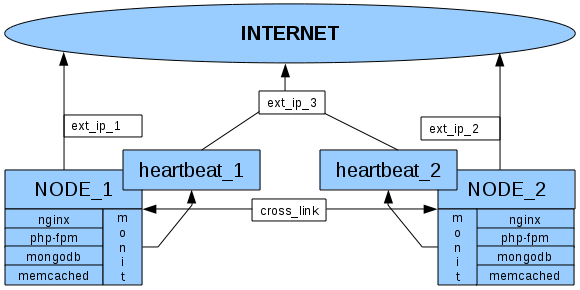
\includegraphics[width=11cm]{01_2012_heartbeat}
  \label{fig:Volkovich1}
\end{figure}

Для начала поднимаются два сервера NODE\_1 и NODE\_2, на которых запущена работающая версия сайта. Затем на оба сервера подключается heartbeat. Он должен <<держать>> виртуальный адрес virt\_ip и следить за доступностью соседнего сервера, а при сбое на текущем --- передавать virt\_ip heartbeat'у соседнего сервера. Однако, этого не достаточно для полного отслеживания того, работает ли сайт, поскольку heartbeat не обладает возможностью проверять работоспособность базы данных mongodb либо других используемых сервисов. Эти задачи можно делегировать демону monit, настроенному для проверки того, работают ли все необходимые демоны.

На данном этапе конфигурация, в принципе, является завершенной, и если какой-то из демонов на мастер-сервере <<упадет>>, обслуживание сайта немедленно будет перенаправлено на второй сервер. Но, как показала практика, и этого оказывается недостаточно в случае, когда демон работает, но при этом выдает неверные данные, либо просто зависает, захватив все наличные ресурсы. Для решения данной проблемы нами было написано несколько небольших скриптов, которые запускаются по cron'у и проверяют такие параметры, как репликацию в memcached и mongodb, отдачу http-трафика через php-fpm и др. менее значительные нюансы. И в случае, если проверка не проходит, в скрипте (как и в monit) выполняется команда hb\_standby, которая заставляет heartbeat принудительно отдать virt\_ip на slave-сервер, если таковой имеется.

\subsection*{Конфигурация демонов}

Ниже приведены ключевые параметры, использованные нами при конфигурировании:

\subsubsection*{heartbeat}

\begin{itemize}
  \item haresources
%\end{itemize}
\begin{verbatim}
    passport1.pronto.ru IPaddr::194.87.222.180/27/eth0 nginx
\end{verbatim}
%\begin{itemize}
  \item ha.cf
%\end{itemize}
\begin{verbatim}
    debugfile /var/log/ha-debug
    logfile /var/log/ha-log
    logfacility local0
    keepalive 2
    deadtime 30
    warntime 10
    initdead 120
    udpport 694
    ucast eth1 192.168.0.2
    auto_failback off
    node passport1.pronto.ru passport2.pronto.ru
    ping_group ping_nodes 8.8.8.8
    respawn hacluster /usr/lib/heartbeat/ipfail
    deadping 30
    use_logd yes
    debug 1
\end{verbatim}
\end{itemize}
\subsubsection*{monit}

\begin{itemize}
  \item monitrc
%\end{itemize}
\begin{verbatim}
    check process nginx
    with pidfile "/var/run/nginx.pid"
    start program = "/etc/init.d/nginx start"
    stop program = "/etc/init.d/nginx stop"
    group www
\end{verbatim}
\end{itemize}
\subsection*{Тестирование}

При проверке работоспособности системы мы использовали следующие способы нарушения работоспособности сайта:

\begin{itemize}
  \item моментальное отключение питания на мастер-ноде;
  \item падение интерфейса на мастер-ноде;
  \item падение любого из демонов, обслуживающего сайт;
  \item нарушение репликации memcached и mongodb.
\end{itemize}

Результатом любого из перечисленных событий являлось

\begin{itemize}
  \item моментальное переключение ip-адреса сайта на соседний сервер;
  \item отправка администраторам уведомлений обо всех событиях.
\end{itemize}


\begin{thebibliography}{9}

\bibitem{Volkovich1} \url{http://www.linux-ha.org}

\bibitem{Volkovich2} \url{http://mmonit.com/monit}

\bibitem{Volkovich3} \url{http://sysoev.ru/nginx}

\bibitem{Volkovich4} \url{http://php-fpm.org}

\bibitem{Volkovich5} \url{http://www.mongodb.org}

\bibitem{Volkovich6} \url{http://memcached.org}

\end{thebibliography}

\end{document}





\documentclass[10pt, a5paper]{article}
\usepackage{pdfpages}
\usepackage{parallel}
\usepackage[T2A]{fontenc}
\usepackage{ucs}
\usepackage[utf8x]{inputenc}
\usepackage[polish,english,russian]{babel}
\usepackage{hyperref}
\usepackage{rotating}
\usepackage[inner=2cm,top=1.8cm,outer=2cm,bottom=2.3cm,nohead]{geometry}
\usepackage{listings}
\usepackage{graphicx}
\usepackage{wrapfig}
\usepackage{longtable}
\usepackage{indentfirst}
\usepackage{array}
\newcolumntype{P}[1]{>{\raggedright\arraybackslash}p{#1}}
\frenchspacing
\usepackage{fixltx2e} %text sub- and superscripts
\usepackage{icomma} % коскі ў матэматычным рэжыме
\PreloadUnicodePage{4}

\newcommand{\longpage}{\enlargethispage{\baselineskip}}
\newcommand{\shortpage}{\enlargethispage{-\baselineskip}}

\def\switchlang#1{\expandafter\csname switchlang#1\endcsname}
\def\switchlangbe{
\let\saverefname=\refname%
\def\refname{Літаратура}%
\def\figurename{Іл.}%
}
\def\switchlangen{
\let\saverefname=\refname%
\def\refname{References}%
\def\figurename{Fig.}%
}
\def\switchlangru{
\let\saverefname=\refname%
\let\savefigurename=\figurename%
\def\refname{Литература}%
\def\figurename{Рис.}%
}

\hyphenation{admi-ni-stra-tive}
\hyphenation{ex-pe-ri-ence}
\hyphenation{fle-xi-bi-li-ty}
\hyphenation{Py-thon}
\hyphenation{ma-the-ma-ti-cal}
\hyphenation{re-ported}
\hyphenation{imp-le-menta-tions}
\hyphenation{pro-vides}
\hyphenation{en-gi-neering}
\hyphenation{com-pa-ti-bi-li-ty}
\hyphenation{im-pos-sible}
\hyphenation{desk-top}
\hyphenation{elec-tro-nic}
\hyphenation{com-pa-ny}
\hyphenation{de-ve-lop-ment}
\hyphenation{de-ve-loping}
\hyphenation{de-ve-lop}
\hyphenation{da-ta-ba-se}
\hyphenation{plat-forms}
\hyphenation{or-ga-ni-za-tion}
\hyphenation{pro-gramming}
\hyphenation{in-stru-ments}
\hyphenation{Li-nux}
\hyphenation{sour-ce}
\hyphenation{en-vi-ron-ment}
\hyphenation{Te-le-pathy}
\hyphenation{Li-nux-ov-ka}
\hyphenation{Open-BSD}
\hyphenation{Free-BSD}
\hyphenation{men-ti-on-ed}
\hyphenation{app-li-ca-tion}

\def\progref!#1!{\texttt{#1}}
\renewcommand{\arraystretch}{2} %Іначай формулы ў матрыцы зліпаюцца з лініямі
\usepackage{array}

\def\interview #1 (#2), #3, #4, #5\par{

\section[#1, #3, #4]{#1 -- #3, #4}
\def\qname{LVEE}
\def\aname{#1}
\def\q ##1\par{{\noindent \bf \qname: ##1 }\par}
\def\a{{\noindent \bf \aname: } \def\qname{L}\def\aname{#2}}
}

\def\interview* #1 (#2), #3, #4, #5\par{

\section*{#1\\{\small\rm #3, #4. #5}}

\def\qname{LVEE}
\def\aname{#1}
\def\q ##1\par{{\noindent \bf \qname: ##1 }\par}
\def\a{{\noindent \bf \aname: } \def\qname{L}\def\aname{#2}}
}


\begin{document}

\title{Параўнальны аналіз выкарыстання свабоднага праграмнага забеспячэння ў ВНУ Беларусі, Расійскай Федэрацыі і Украіны}%\footnote{Текст данных и последующих тезисов, кроме специально оговоренных случаев, доступен под лицензией Creative Commons Attribution-ShareAlike 3.0}

\author{Е. Аляксееў\footnote{Донецк, Украина}, Г. Злобін\footnote{Львов, Украина}, Д. Костюк\footnote{Брест, Беларусь}}
\maketitle

\begin{abstract}
The report presents a comparative analysis of FOSS usage in higher educational institutions of Belarus, Russia and Ukraine on the basis of the FOSS Lviv-2011 and FOSS Lviv-2012 conferences materials. System software of workstations is reviewed as well as auxiliary software used by students and software studied in the academic process.
\end{abstract}

Стварэнне ў 1981 г. фірмай IBM персанальнай ЭВМ IBM PC з адкрытай архітэктурай справакавала з'яўленне IBM-сумяшчальных ПЭВМ, якія вырабляліся ў многіх краінах свету. Не адсталі ад гэтых краін СССР і краіны Савета эканамічнай узаемадапамогі, якія сталі вырабляць цэлы спектр такіх ПЭВМ:

\begin{itemize}
  \item ЕС 1840, ЕС 1841, Іскра 1030, Нейроны (СССР);
  \item ЕС 1834, ЕС 1835 (ГДР);
  \item ЕС 1839 (НРБ).
\end{itemize}

Для ПЭВМ савецкай вытворчасці была створана рускамоўная аперацыйная сістэма АльфаДОС, тэкставы рэдактар Лексікон, тэкставы рэдактар Text tip (Балгарыя), тэкставы працэсар Нейроны"=тэкст, таблічны працэсар Нейроны"=рахунак, СКБД Нейроны"=база. Цяжка сказаць, наколькі ліцэнзійна-чыстымі былі АльфаДОС, Нейрон"=тэкст, Нейрон"=рахунак, Нейрон"=база, бо дзякуючы <<жалезнай заслоне>> прымяніць да СССР санкцыі з нагоды парушэнняў аўтарскіх правоў уласнікаў праграм было няпроста. Неўзабаве пасля развалу СССР дзякуючы падзенню <<жалезнай заслоны>> ў многіх краінах СНД пачалася зборка IBM"=сумяшчальных ЭВМ з камплектуючых, увезеных у асноўным з краін паўднёва"=ўсходняй Азіі. На гэтыя ПЭВМ усталёўваліся пераважна пірацкія версіі як сістэмнага, так і прыкладнога праграмнага забеспячэння. Відавочна, што каштавалі гэтыя ПЭВМ значна танней аналагічных ПЭВМ еўрапейскай і амерыканскай вытворчасці, не кажучы ўжо пра ПЭВМ фірмы Apple. З"=за гэтага аперацыйная сістэма MS DOS і офісны пакет Microsoft Office сталі дэ-факта стандартам у ВНУ краін СНД. Ці садзейнічала распаўсюджванню пірацкага ПЗ у ВНУ СНД адсутнасць заканадаўства аб абароне аўтарскіх правоў уласнікаў праграм зараз сказаць цяжка, але разам з тым амаль 10 гадоў мы без абмежаванняў капіявалі і ўсталёўвалі пірацкія копіі прапрыетарнага ПЗ.

У Беларусі, Расійскай Федэрацыі і Украіне законы аб абароне аўтарскіх правоў уласнікаў праграм уведзены з 1996 г. (Беларусь), з 2001 г. (Украіна). У Расійскай Федэрацыі з 1993 г. дзейнічаў закон аб аўтарскім праве і сумежных правах, які страціў моц з 1 студзеня 2008 года ў сувязі з уступленнем у сілу чацвёртай часткі Грамадзянскага кодэкса РФ. Зрэшты гэта мала паўплывала на сітуацыю з пірацкім ПЗ у ВНУ гэтых краін. Выпадкі пераследу ВНУ за парушэнні аўтарскіх правоў у вобласці праграмнага забеспячэння былі малалікімі і не заўсёды яны праводзіліся з мэтай абароны аўтарскіх правоў уласнікаў праграм. Аднак ужыванне законаў аб абароне аўтарскіх правоў уласнікаў праграм да суб'ектаў гаспадарчай дзейнасці стала ствараць ціск на ВНУ: <<Вучыце сваіх выпускнікоў таму, з чым яны будуць працаваць на нашых працоўных месцах>>. Шмат фірмаў спачатку пераходзіць на СПЗ з мэтай памяншэння сумы ліцэнзійных адлічэнняў уласнікам прапрыетарнага ПЗ.

Яшчэ адным аргументам на карысць змены сітуацыі з выкарыстаннем ВПЗ у ВНУ Беларусі, Расійскай Федэрацыі і Украіны стал пачатак эры мабільных працоўных месцаў --- цяжка прадбачыць, якая АС і якое прыкладное ПЗ будзе ўстаноўлена на нэтбуке, планшэце ці смартфоне супрацоўніка фірмы. З'яўленне мабільных працоўных месцаў і хуткая змена версій сістэмнага і прыкладнога ПЗ змушае ВНУ да адмовы ад тэхналагічнай накіраванасці лекцыйных курсаў, звязаных з кампутарным тэхналогіямі, на карысць фундаментальнага складніка. А гэта прыводзіць да з'яўлення меркаванняў тыпу <<Калі мы павінны навучыць студэнтаў асновам працы з графічным інтэрфейсам ў любой АС, то чаму гэта павінна быць дарагая Microsoft Windows? Мэтазгодней рабіць гэта ў свабоднай і бясплатнай GNU/Linux?>> Разам з тым, адмова ад напрацовак метадычнага забеспячэння для выкладчыкаў ВНУ з'яўляецца даволі няпростым працэсам, асабліва ва ўмовах безадказнасці за выкарыстанне пірацкага ПЗ. За час ад падпісання Белавежскага пагаднення аб спыненні існавання СССР Беларусь, Расійская Федэрацыя і Украіна прайшлі кожная свой шлях развіцця і было б цікава параўнаць стан з выкарыстаннем ВПЗ у ВНУ гэтых краін.

\subsection*{І. Выкарыстанне ВПЗ ў ВНУ Беларусi}

Сёння рынак працы Беларусі патрабуе вывучэння многіх прапрыетарных праграмных прадуктаў, пачынаючы ад платформы Microsoft Windows і скончваючы спецыялізаванымі CAD/CAM"=сістэмамі. Гэтая тэндэнцыя суправаджаецца слабай матывацыяй выкарыстання СПЗ, якая абумоўлена тым, што рызыка парушэння ліцэнзіі як і раней застаецца ў вобласці здагадак без рэальных дзеянняў беларускіх кантралюючых органаў. Доля легальна набытага ПЗ узрасла ў апошнія гады за кошт спецыяльных скідак ад пастаўшчыкоў, а таксама праз высокія эканамічныя паказчыкі да 2011 г. Тым не менш, эканамічны фактар не з'яўляецца вырашальным для прыняцця выбару паміж свабодным ПЗ і прапрыетарным. Таму выкарыстанне СПЗ у ВНУ звычайна абумоўлена яго тэхнічнымі перавагамі ў параўнанні з прапрыетарнымі аналагамі або патрабаваннямі рынку працы. Выбар ПЗ сервера можа быць адзіным выключэннем, паколькі ён істотна залежыць ад асабістых густаў сістэмных адміністратараў.

У апошнія гады назіраецца рост цікаўнасці карпаратыўных працадаўцаў да GNU/Linux, пераважна для ўбудавальных і серверных сістэм. У сувязі з гэтым буйныя гульцы рынку актыўна заяўляюць аб сваіх уласных трэнінгах і семінарах, прысвечаных гэтай тэме.

Выкарыстанне СПЗ у ВНУ Беларусі можна падзяліць на тры напрамкі:

\begin{enumerate}
  \item \textbf{ПЗ падтрымкі навучальнага працэсу (пераважна сістэмнае ПЗ на серверах і працоўных станцыях).} У большасці выпадкаў сістэмнае СПЗ на працоўных станцыях прадстаўлена GNU/Linux у рэжыме мультызагрузкі ў якасці альтэрнатыўнай АС у кампутарных класах кафедраў, якія навучаюць праграмаванню студэнтаў інжынерных спецыялізацый. У педагагічных ВНУ GNU/Linux на настольных кампутарах выкарыстоўваецца рэдка ў сувязі з недастатковай распаўсюджанасцю GNU/Linux у школах Беларусі. Разам з тым у некаторых універсітэтах заўважана выкарыстанне Linux у тонкіх кліентах з тэрмінальным Windows-серверам (напрыклад, Гродзенскі дзяржуніверсітэт імя Янкі Купалы);
  \item \textbf{дадатковае ПЗ, якое выкарыстоўваецца студэнтамі ў самастойнай працы.} Да гэтай групы ПЗ можна залічыць офісны пакет OpenOffice.org і браўзэр Firefox;
  \item \textbf{ПЗ для выкарыстання ў навучальных курсах.} У гэтым кірунку СПЗ пераважна выкарыстоўваюць у інжынерных ВНУ, асабліва тых, якія вядуць навучанне ІТ-спецыялістаў, а менавіта СПЗ для навучання праграмавання на мовах Асэмблер, C++, Java і PHP, SciLab для выканання матэматычных разлікаў, QCAD/LibreCAD, Blender, cirquit CAD для вывучэння сістэм аўтаматызаванага праектавання, выкарыстанне свабодных сістэм віртуалізацыі VirtualBox і KVM для вывучэння аперацыйных сістэм, выкарыстанне Moodle і iTest для тэставай праверкі ведаў студэнтаў.
\end{enumerate}

Асобна трэба падкрэсліць выкарыстанне СПЗ для кластараў і нацыянальнай ГРІД-сістэмы Беларусі, у якую ўключаны рэсурсы вядучых універсітэтаў (Беларускі дзяржуніверсітэт, Гродзенскі дзяржуніверсітэт імя Янкі Купалы, Беларускі дзяржуніверсітэт інфарматыкі і радыёэлектронікі, Беларускі нацыянальны тэхнічны універсітэт), навуковых устаноў і прадпрыемстваў краіны ў рамках сумеснай расійска-беларускай праграмы СКІФ-ГРІД.

Выкарыстанне СПЗ у ВНУ Беларусі можна праілюстраваць наступным малюнкам

\begin{figure}[htpb]
  \centering
  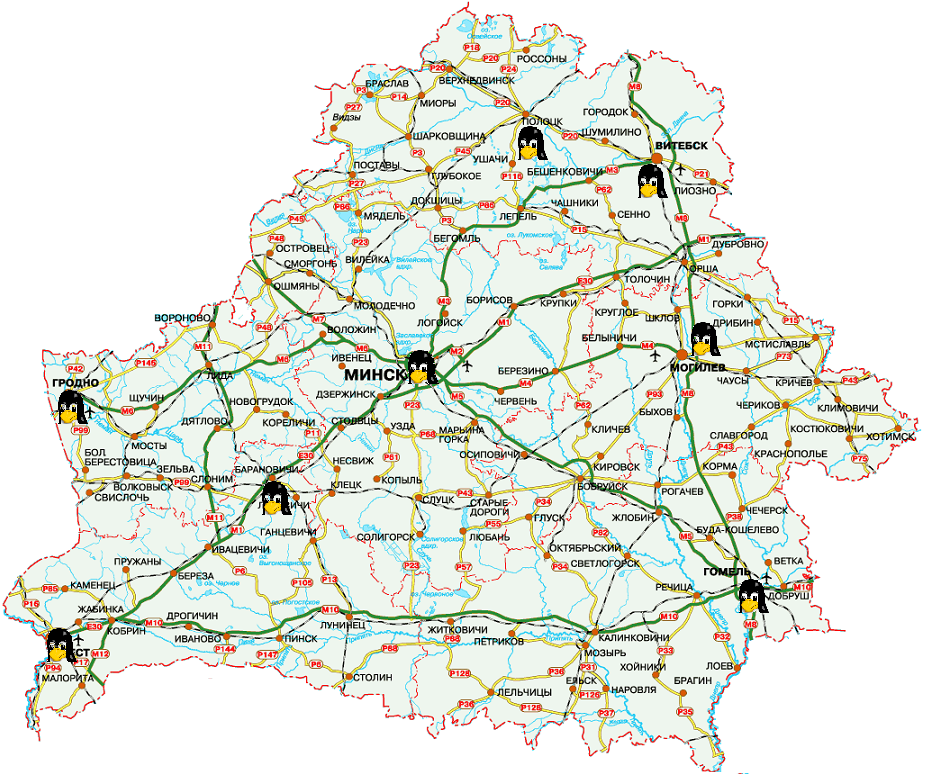
\includegraphics[width=7cm]{03_2012_bilorus}
  \label{fig:Zlobin1}
  \caption{Выкарыстанне СПЗ у ВНУ Беларусі}
\end{figure}


\subsection*{ІІ. Выкарыстанне СПЗ ў ВНУ Расійскай Федэрацыі}

У адрозненні ад Беларусі ў Расійскай Федэрацыі ў 2008 г. была прынята канцэпцыя развіцця распрацоўкі і выкарыстання свабоднага праграмнага забеспячэння. У рамках гэтай канцэпцыі ў 2008-2010 гг. была рэалізавана праграма выкарыстання СПЗ у школах Расійскай Федэрацыі (у 35\% школ СПЗ устаноўлена больш чым на 50\% кампутараў). Трэба адзначыць, што ў адрозненне ад Беларусі і Украіны ў Расійскай Федэрацыі назіраецца некаторая актыўнасць кантралюючых органаў з нагоды ліцэнзійнага праграмнага забеспячэння. Самай рэзананснай справай была справа А.М. Понасава, якая і прывяла да стварэння ў 2008 г. грамадскай арганізацыі <<Цэнтр вольных тэхналогій>>. Як вынікае з  \cite{Zlobin1, Zlobin2, Zlobin3}, у большасці ВНУ Расійскай Федэрацыі назіраецца выкарыстанне як Microsft Windows, так і GNU/Linux. Толькі ў некаторых ВНУ кіраўніцтвам прынята валявое рашэнне аб поўным пераходзе на СПЗ (Санкт-Пецярбургскі гандлёва-эканамічны універсітэт, Томскі дзяржаўны педагагічны універсітэт, Ніжагародскі радыётэхнічны каледж). Як і ў Беларусі выкарыстанне СПЗ у ВНУ Расійскай Федэрацыі можна падзяліць на тры напрамкі \cite{Zlobin3, Zlobin4, Zlobin5}:

\begin{enumerate}
  \item \textbf{праграмнае забеспячэнне падтрымкі навучальнага працэсу} (у асноўным сістэмнае праграмнае забеспячэнне на серверах і працоўных станцыях). У большасці выпадкаў сістэмнае СПЗ на працоўных станцыях прадстаўлена GNU/Linux у рэжыме мультызагрузкі як альтэрнатыўная АС у кампутарных класах кафедраў;
  \item \textbf{дадатковае праграмнае забеспячэнне, якое выкарыстоўваецца студэнтамі пры самастойнай працы} (на жаль аўтары не валодаюць дадзенымі аб гэтай групе СПЗ);
  \item \textbf{праграмнае забеспячэнне для выкарыстання ў навучальных курсах.} У гэтым кірунку спектр СПЗ значна шырэй, чым у Беларусі. Тут можна згадаць выкарыстанне СПЗ для вывучэння праграмавання на мовах С/C++ (у Яраслаўскім Універсітэце ёсць цікавы вопыт навучання праграмаванню на аснове СПЗ), Pascal (Free Pascal, Lazarus), Java, Haskel, Prolog; SciLab, Octave, Sage для выканання матэматычных разлікаў (шырокі вопыт выкарыстання вольнага матэматычнага праграмнага забеспячэння назапашаны ва універсітэтах Новасібірска, Барнаула, Бійска); арганізацыя сістэм дыстанцыйнага навучання, выкарыстанне свабодных сістэм віртуалізацыі для вывучэння аперацыйных сістэм; інструментар для філалагічнага аналізу тэкстаў; выкарыстанне інструментара верыфікацыі ПЗ у падрыхтоўцы магістраў; стварэнне электронных адукацыйных рэсурсаў падтрымкі навучальнага працэсу для завочнай формы навучання (аўтары разумеюць, што рэальны спіс выкарыстанага СПЗ значна шырэй, але ў адкрытым доступе дадзеных пакуль што няма).
\end{enumerate}

У ВНУ Расійскай Федэрацыі даволі актыўна выкарыстоўваюцца вылічальныя кластары з выкарыстаннем СПЗ. Па ініцыятыве рэктараў МДУ ім. М.В. Ламаносава, Ніжагародскага універсітэта ім. М.І. Лабачэўскага, Томскага дзяржаўнага універсітэта, Паўднёва-Уральскага дзяржаўнага універсітэта створаны <<Суперкампутарны кансорцыум універсітэтаў Расіі>>. У спіс TOP500 ад снежня 2011 г. уваходзяць чатыры расейскія суперкампутара (\No \No 18, 107, 119, 121).

Варта адзначыць, што ў Расійскай Федэрацыі назапашаны значны вопыт распрацоўкі свабоднага праграмнага забеспячэння. У Расеі распрацоўваюцца дыстрыбутывы GNU/Linux: ALT Linux (\url{http://altlinux.ru}), Calculate Linux (\url{http://www.calculate-linux.ru}), ROSA (\url{http://rosalab.ru}). Наяўнасць кампаній, якія займаюцца распрацоўкай СПЗ, дазваляе распрацоўваць спецыялізаваныя свабодныя праграмы і значна спрашчае рэалізацыю праектаў па ўкараненні GNU/Linux у школы і універсітэты.

\begin{figure}[htpb]
  \centering
  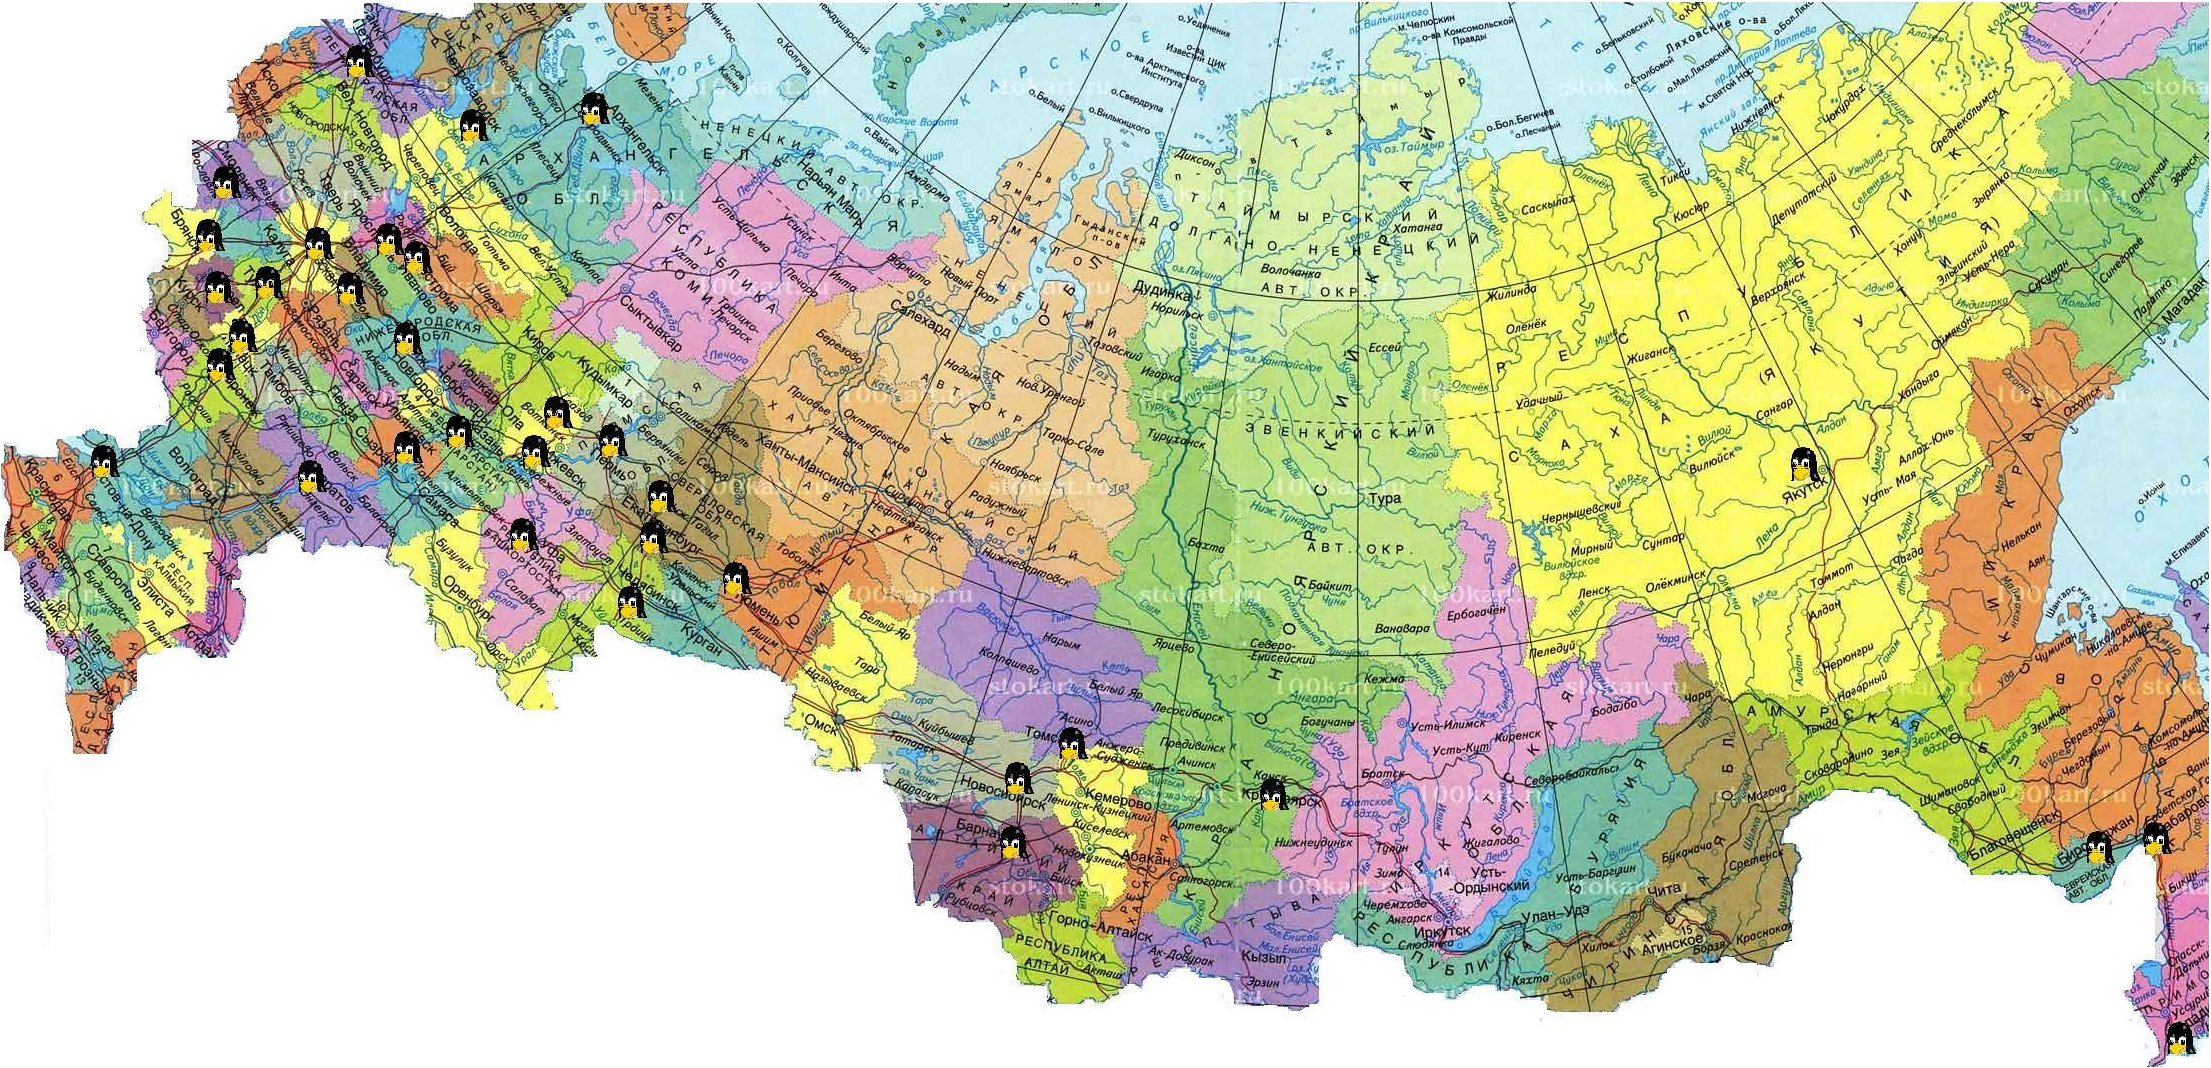
\includegraphics[width=11cm]{03_2012_russia2_with_tux}
  \label{fig:Zlobin2}
  \caption{Выкарыстанне СПЗ у ВНУ Расійскай Федэрацыі}
\end{figure}

\subsection*{ІІІ. Выкарыстанне СПЗ у ВНУ Украіны}

Ва Украіне <<Дзяржаўная мэтавая навукова-тэхнічная праграма выкарыстання ў органах улады праграмнага забеспячэння з адкрытым кодам>> была зацверджана ў 2010 г., але да рэальнага яе выканання пакуль што не дайшлі. У адрозненне ад Расійскай Федэрацыі праверкі адпаведнымі дзяржаўнымі органамі выпадкаў парушэння аўтарскіх правоў уласнікаў праграм праводзяцца ў значна меншым аб'ёме і пераважна ў гасразліковых арганізацыях. Вядомыя толькі асобныя выпадкі такіх праверак у ВНУ. Як і ў Беларусі пакуль што адсутнічае эканамічны складнік у выбары праграмнага забеспячэння для ВНУ. Пасля набыцця ПЭВМ пераважна з ліцэнзійнымі Microsoft Windows і Microsoft Office устанаўліваецца вялікая колькасць неліцэнзійнага ПЗ, чым зводзяцца дарэмна фантастычна вялікія выдаткі сродкаў на першаснае набыццё ПА (Львоўскі нацыянальны універсітэт імя Івана Франка да эканамічнага крызісу 2008 г. кожны год купляў прыблізна 1000 ПЭВМ. Сумарній кошт ліцэнзій толькі на Microsoft Windows (ОЭМ-версія) і Microsoft Office складал амаль 300000 у.а. на год--даволі вялікая сума, як для ЛНУ ім.і.Франка!). У большасці выпадкаў выбар менавіта прапрыетарнага ПЗ звязаны нават не са спажывецкімі якасцямі гэтых праграм, а фактам павярхоўнага знаёмства выкладчыка з гэтай праграмай ці нават наяўнасцю ў яго якой-небудзь кніжкі з апісаннем праграмы. Разам з тым, выступленні выкладчыкаў і навуковых супрацоўнікаў на першай і другой канферэнцыі FOSS Lviv  \cite{Zlobin1, Zlobin2} сведчаць аб шырокім спектры выкарыстання СПЗ у ВНУ Украіны.

Як і ў Беларусі і Расійскай Федэрацыі выкарыстанне СПЗ у ВНУ Украіны можна падзяліць на тры напрамкі \cite{Zlobin1, Zlobin2}:

\begin{enumerate}
  \item \textbf{праграмнае забеспячэнне падтрымкі навучальнага працэсу (у асноўным сістэмнае праграмнае забеспячэнне на серверах і працоўных станцыях).} У большасці выпадкаў сістэмнае СПЗ на працоўных станцыях прадстаўлена GNU/Linux у рэжыме мультызагрузкі, як альтэрнатыўная АС у кампутарных класах кафедраў;
  \item \textbf{дадатковае праграмнае забеспячэнне, якое выкарыстоўваецца студэнтамі падчас іх самастойнай працы} (на жаль, аўтары на сённяшні дзень не маюць дадзеных аб гэтай групе СПЗ);
  \item \textbf{праграмнае забеспячэнне для выкарыстання ў навучальных курсах.} У гэтым кірунку спектр СПЗ значна шырэй, чым у Беларусі. Гэта выкарыстанне сістэм кампутарнай матэматыкі; арганізацыя сістэм дыстанцыйнага навучання, выкарыстанне свабодных сістэм віртуалізацыі для вывучэння аперацыйных сістэм; выкарыстанне СПЗ для тэставання апаратнага забеспячэння ПЭВМ; выкарыстанне офіснага пакета OpenOffice.org.ukr у курсе інфарматыкі ВНУ; выкарыстанне адкрытых сродкаў праграмавання ў навучанні і ў навуковых даследаваннях; (аўтары аддаюць сабе справаздачу ў тым, што рэальны спіс прымяняемага СПЗ значна шырэй, але больш поўныя дадзеныя аб гэтым аўтарам невядомыя).
\end{enumerate}

У ВНУ Украіны эксплуатуюцца вылічальныя кластары с выкарыстаннем СПЗ, нараўне са спецыялізаванымі ўстаноўкамі шырока выкарыстоўваюцца размеркаваныя кластарныя сістэмы і сістэмы з выкананнем вылічэнняў на графічных працэсарах.

У выніку можна канстатаваць як шырокі спектр выкарыстання СПЗ ва ўкраінскіх ВНУ ад дыстанцыйнага навучання да распрацоўкі СПЗ, так і шырокую геаграфію выкарыстання СПЗ ад Луганска на ўсходзе да Львова на захадзе і ад Чарнігава на поўначы да Адэсы на поўдні.

\begin{figure}[htpb]
  \centering
  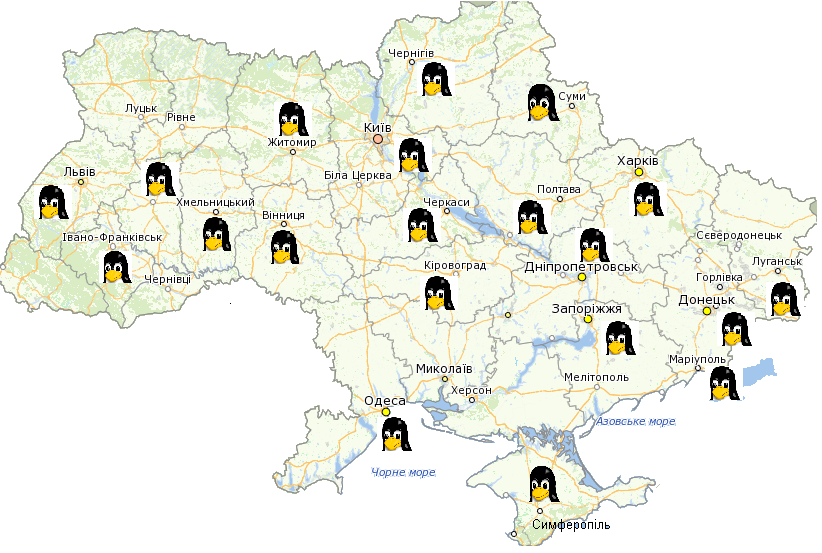
\includegraphics[width=07cm]{03_2012_ukraine}
  \label{fig:Zlobin3}
  \caption{Выкарыстанне СПЗ у ВНУ Украіны}
\end{figure}

Падводзячы вынікі, можна канстатаваць, што:

\begin{enumerate}
  \item незалежна ад наяўнасці або адсутнасці канцэпцыі выкарыстання СПЗ, яно выкарыстоўваецца ў ВНУ Беларусі, Расійскай Федэрацыі і Украіны;
  \item колькасна аб'ём выкарыстання СПЗ у адукацыі вышэй у Расійскай Федэрацыі;
  \item ва ўсіх трох краінах міністэрства адукацыі займаюць адхіленую пазіцыю ў працэсе ўкаранення СПЗ ва універсітэты і школы;
  \item ва ўсіх трох краінах узровень выкарыстання СПЗ у ВНУ з'яўляецца недастатковым. Свабода выбару ПЗ, якой карыстаюцца выкладчыкі ВНУ, у большасці выпадкаў не прыводзіць да выбару найлепшага інструментара, а абумоўлена звычкамі альбо стэрэатыпамі (часта памылковымі) выкладчыкаў.
\end{enumerate}

\let\saverefname=\refname
\def\refname{Літаратура}
\begin{thebibliography}{9}

\bibitem{Zlobin1} Тези доповідей міжнародної науково-практичної конференції FOSS Lviv-2011. --- Львів.: Львівський національний університет імені Івана Франка, 2011. --- 196 с.

\bibitem{Zlobin2} Друга міжнародна науково-практична конференція FOSS Lviv-2012: Збірник наукових праць/ Львів, 26-28 квітня 2012 р. --- 160 с.

\bibitem{Zlobin3} Алексеев Е.Р., Брагилевский В.Н. Использование свободного програмного обеспечения в университетах и исследовательских учреждений Российской Федерации. Друга міжнародна науково-практична конференція FOSS Lviv-2012: Збірник наукових праць/ Львів, 26-28 квітня 2012 р.

\bibitem{Zlobin4} В.Н. Брагилевский, С.А. Гуда, Г.В. Худолей СПО на мехмате Южного федерального университета. Седьмая конференция <<Свободное программное обеспечение в высшей школе>>: Тезисы докладов/ Переславль, 28-29 января 2012 года. М.: Альт Линукс, 2012. 110 с.: ил.

\bibitem{Zlobin5} \url{http://lists.raspo.ru/Plone/publichnye-drafty-dokumentov/dokumenty-komiteta-po-obrazovaniyu-i-vysshei-shkole/spo-v-rossiiskih-vuzah}

\bibitem{Zlobin6} Derechennik S.S., Kostiuk D.A., Pynkin D.A. Free/libre software usage in the belarusian system of higher educational institutions // Друга міжнародна науково-практична конференція FOSS Lviv-2012: Збірник наукових праць/ Львів, 26-28 квітня 2012 р.

\end{thebibliography}
\let\refname=\saverefname

\end{document}





\documentclass[10pt, a5paper]{article}
\usepackage{pdfpages}
\usepackage{parallel}
\usepackage[T2A]{fontenc}
\usepackage{ucs}
\usepackage[utf8x]{inputenc}
\usepackage[polish,english,russian]{babel}
\usepackage{hyperref}
\usepackage{rotating}
\usepackage[inner=2cm,top=1.8cm,outer=2cm,bottom=2.3cm,nohead]{geometry}
\usepackage{listings}
\usepackage{graphicx}
\usepackage{wrapfig}
\usepackage{longtable}
\usepackage{indentfirst}
\usepackage{array}
\newcolumntype{P}[1]{>{\raggedright\arraybackslash}p{#1}}
\frenchspacing
\usepackage{fixltx2e} %text sub- and superscripts
\usepackage{icomma} % коскі ў матэматычным рэжыме
\PreloadUnicodePage{4}

\newcommand{\longpage}{\enlargethispage{\baselineskip}}
\newcommand{\shortpage}{\enlargethispage{-\baselineskip}}

\def\switchlang#1{\expandafter\csname switchlang#1\endcsname}
\def\switchlangbe{
\let\saverefname=\refname%
\def\refname{Літаратура}%
\def\figurename{Іл.}%
}
\def\switchlangen{
\let\saverefname=\refname%
\def\refname{References}%
\def\figurename{Fig.}%
}
\def\switchlangru{
\let\saverefname=\refname%
\let\savefigurename=\figurename%
\def\refname{Литература}%
\def\figurename{Рис.}%
}

\hyphenation{admi-ni-stra-tive}
\hyphenation{ex-pe-ri-ence}
\hyphenation{fle-xi-bi-li-ty}
\hyphenation{Py-thon}
\hyphenation{ma-the-ma-ti-cal}
\hyphenation{re-ported}
\hyphenation{imp-le-menta-tions}
\hyphenation{pro-vides}
\hyphenation{en-gi-neering}
\hyphenation{com-pa-ti-bi-li-ty}
\hyphenation{im-pos-sible}
\hyphenation{desk-top}
\hyphenation{elec-tro-nic}
\hyphenation{com-pa-ny}
\hyphenation{de-ve-lop-ment}
\hyphenation{de-ve-loping}
\hyphenation{de-ve-lop}
\hyphenation{da-ta-ba-se}
\hyphenation{plat-forms}
\hyphenation{or-ga-ni-za-tion}
\hyphenation{pro-gramming}
\hyphenation{in-stru-ments}
\hyphenation{Li-nux}
\hyphenation{sour-ce}
\hyphenation{en-vi-ron-ment}
\hyphenation{Te-le-pathy}
\hyphenation{Li-nux-ov-ka}
\hyphenation{Open-BSD}
\hyphenation{Free-BSD}
\hyphenation{men-ti-on-ed}
\hyphenation{app-li-ca-tion}

\def\progref!#1!{\texttt{#1}}
\renewcommand{\arraystretch}{2} %Іначай формулы ў матрыцы зліпаюцца з лініямі
\usepackage{array}

\def\interview #1 (#2), #3, #4, #5\par{

\section[#1, #3, #4]{#1 -- #3, #4}
\def\qname{LVEE}
\def\aname{#1}
\def\q ##1\par{{\noindent \bf \qname: ##1 }\par}
\def\a{{\noindent \bf \aname: } \def\qname{L}\def\aname{#2}}
}

\def\interview* #1 (#2), #3, #4, #5\par{

\section*{#1\\{\small\rm #3, #4. #5}}

\def\qname{LVEE}
\def\aname{#1}
\def\q ##1\par{{\noindent \bf \qname: ##1 }\par}
\def\a{{\noindent \bf \aname: } \def\qname{L}\def\aname{#2}}
}


\begin{document}

\title{Software security}%\footnote{Текст данных и последующих тезисов, кроме специально оговоренных случаев, доступен под лицензией Creative Commons Attribution-ShareAlike 3.0}

\author{Алексей Чеусов\footnote{Минск, Беларусь}}
\maketitle

\begin{abstract}
System techniques and methods are reviewed for securing the software in UNIX World.
\end{abstract}

Язык программирования С, на десятилетия определивший успех операционных систем класса UNIX, на протяжении последних лет все чаще
становится источником проблем в области безопасности программного
обеспечения. Появившись как язык системного программирования, язык С
широко применяется также и для разработки прикладного ПО, что, ввиду принципиальной <<небезопасности>> этого языка, приводит к многочисленным проблемам, таким как получение доступа к системе злоумышленником, повышению привилегий процесса до уровня суперпользователя, rootkit-ам, нестабильности работы ОС и т.п. То же относится и к языку программирования С++.

В ближайшее время вряд ли стоит ожидать значительного падения популярности этих языков в области разработки как системного, так и прикладного ПО, поэтому
актуальной становится разработка средств и методов борьбы с
перечисленными выше проблемами менее радикальными, чем смена языка
программирования, средствами. Таким средствам и технологиям, существующим и развивающимся в различных UNIX"=подобных системах, посвящен настоящий краткий обзор.

К числу рассматриваемых технологий защиты можно среди прочих отнести следующие:

\begin{itemize}
  \item безопасные функции strl\{cat,cpy\} для работы со строками,
  \item SSP (stack smashing protection) "--- защита от переполнения стека,
  \item ASLR (address space layout randomization) "--- рандомизация базовых адресов сегментов виртуальной памяти процесса,
  \item PIE (position independent executable) "--- позиционно"=независимые исполняемые файлы,
  \item hardened chroot "--- усиленный chroot,
  \item W\^{}X "--- защита исполняемых сегментов памяти от записи и записываемых (стек и данные) от исполнения,
  \item PaX MPROTECT "--- защита mprotect(2),
  \item PaX Segvgard "--- защита от перебора адресов сегментов памяти приложения,
  \item Information filtering "--- сокрытие информации, доступной пользователям и процессам,
  \item per-user /tmp directory "--- размещение подкаталога временных файлов в домашней директории пользователя,
  \item SUID/SGIG executables "--- избавление от исполняемых файлов с установленным битом SUID,
  \item PAM tcb "--- замена PAM unix как средство избавления от бита SUID у passwd(8)
  \item capsicum "--- расширение POSIX API для обеспечения лучшей безопасности в системе UNIX.
  \item FUSE, PUFFS "--- подсистемы для реализации файловых систем в пространстве пользователя
  \item Микроядерные ОС "--- класс операционных систем, в которых основные сервисы работают на уровне пользователя, на уровне ядра же работает лишь самое необходимодое, за счет чего достигается надежность и безопасность
  \item RUMP "--- подсистема для запуска ядерного кода в пользовательском приложении
  \item SE Linux "--- подсистема контроля доступа в Linux
  \item kauth(9) "--- подсистема авторизации ядра NetBSD
  \item jail "--- система изоляции и виртуализации FreeBSD
\end{itemize}


\end{document}





\documentclass[10pt, a5paper]{article}
\usepackage{pdfpages}
\usepackage{parallel}
\usepackage[T2A]{fontenc}
\usepackage{ucs}
\usepackage[utf8x]{inputenc}
\usepackage[polish,english,russian]{babel}
\usepackage{hyperref}
\usepackage{rotating}
\usepackage[inner=2cm,top=1.8cm,outer=2cm,bottom=2.3cm,nohead]{geometry}
\usepackage{listings}
\usepackage{graphicx}
\usepackage{wrapfig}
\usepackage{longtable}
\usepackage{indentfirst}
\usepackage{array}
\newcolumntype{P}[1]{>{\raggedright\arraybackslash}p{#1}}
\frenchspacing
\usepackage{fixltx2e} %text sub- and superscripts
\usepackage{icomma} % коскі ў матэматычным рэжыме
\PreloadUnicodePage{4}

\newcommand{\longpage}{\enlargethispage{\baselineskip}}
\newcommand{\shortpage}{\enlargethispage{-\baselineskip}}

\def\switchlang#1{\expandafter\csname switchlang#1\endcsname}
\def\switchlangbe{
\let\saverefname=\refname%
\def\refname{Літаратура}%
\def\figurename{Іл.}%
}
\def\switchlangen{
\let\saverefname=\refname%
\def\refname{References}%
\def\figurename{Fig.}%
}
\def\switchlangru{
\let\saverefname=\refname%
\let\savefigurename=\figurename%
\def\refname{Литература}%
\def\figurename{Рис.}%
}

\hyphenation{admi-ni-stra-tive}
\hyphenation{ex-pe-ri-ence}
\hyphenation{fle-xi-bi-li-ty}
\hyphenation{Py-thon}
\hyphenation{ma-the-ma-ti-cal}
\hyphenation{re-ported}
\hyphenation{imp-le-menta-tions}
\hyphenation{pro-vides}
\hyphenation{en-gi-neering}
\hyphenation{com-pa-ti-bi-li-ty}
\hyphenation{im-pos-sible}
\hyphenation{desk-top}
\hyphenation{elec-tro-nic}
\hyphenation{com-pa-ny}
\hyphenation{de-ve-lop-ment}
\hyphenation{de-ve-loping}
\hyphenation{de-ve-lop}
\hyphenation{da-ta-ba-se}
\hyphenation{plat-forms}
\hyphenation{or-ga-ni-za-tion}
\hyphenation{pro-gramming}
\hyphenation{in-stru-ments}
\hyphenation{Li-nux}
\hyphenation{sour-ce}
\hyphenation{en-vi-ron-ment}
\hyphenation{Te-le-pathy}
\hyphenation{Li-nux-ov-ka}
\hyphenation{Open-BSD}
\hyphenation{Free-BSD}
\hyphenation{men-ti-on-ed}
\hyphenation{app-li-ca-tion}

\def\progref!#1!{\texttt{#1}}
\renewcommand{\arraystretch}{2} %Іначай формулы ў матрыцы зліпаюцца з лініямі
\usepackage{array}

\def\interview #1 (#2), #3, #4, #5\par{

\section[#1, #3, #4]{#1 -- #3, #4}
\def\qname{LVEE}
\def\aname{#1}
\def\q ##1\par{{\noindent \bf \qname: ##1 }\par}
\def\a{{\noindent \bf \aname: } \def\qname{L}\def\aname{#2}}
}

\def\interview* #1 (#2), #3, #4, #5\par{

\section*{#1\\{\small\rm #3, #4. #5}}

\def\qname{LVEE}
\def\aname{#1}
\def\q ##1\par{{\noindent \bf \qname: ##1 }\par}
\def\a{{\noindent \bf \aname: } \def\qname{L}\def\aname{#2}}
}


\begin{document}

\title{Обзор Open Build Service}%\footnote{Текст данных и последующих тезисов, кроме специально оговоренных случаев, доступен под лицензией Creative Commons Attribution-ShareAlike 3.0}

\author{Денис Пынькин\footnote{Минск, Беларусь}}
\maketitle

\begin{abstract}
Open Build Service (OBS) is an open and complete distribution development platform. It provides an infrastructure to create and release open source software for openSUSE and other Linux distributions easily on different hardware architectures. The article describes the architecture and usage of private OBS instance.
\end{abstract}

\section*{Введение}

Зачастую коммерческие проекты базируются на открытых платформах, таких, как различные дистрибутивы Linux. Это означает, что для обеспечения поддержки своего продукта  вендору часто необходимо самостоятельно заниматься поддержкой открытых проектов, входящих в его продукт.

Даже при условии сокращения количества поддерживаемых пакетов до минимума,  необходимого для работы коммерческого программного обеспечения, инженерам приходится заниматься поддержкой сотен сторонних пакетов и приложений.

Системы автоматической сборки значительно облегчают жизнь разработчикам, вынужденным обеспечивать платформу для разработки как открытого,  так и коммерческого программного обеспечения. Одна из лучших по совокупности параметров и возможностей система автоматической сборки общего назначения "--- это Open Build Service, умеющая работать со множеством различных дистрибутивов.

\section*{Архитектура}

Open Build Service можно разделить на серверную часть и клиентскую \cite{Pynkin1}.
OBS поддерживает сборку следующих целей:

\begin{itemize}
  \item rpm/spec;
  \item deb/dsc;
  \item KIWI image.
\end{itemize}

\subsection*{Серверная часть}

Основные задачи, которые решает серверная часть:

\begin{itemize}
  \item обеспечивает доступ к исходному коду приложений;
  \item предоставляет ресурсы для сборки пакетов;
  \item предоставляет инфраструктуру для публикации пакетов;
  \item обеспечивает взаимодействие между разработчиками.
\end{itemize}

В свою очередь OBS-сервер состоит из двух частей:

\begin{itemize}
  \item front-end:
    \begin{itemize}
      \item публичный API для различных клиентов;
      \item доступ к исходникам;
      \item доступ к логам и результатам сборки;
      \item доступ к собранным пакетам;
      \item контроль процесса сборки пакетов;
      \item управление пользователями;
    \end{itemize}


  \item back-end:
    \begin{itemize}
      \item хранилище исходного кода;
      \item сборочная <<ферма>>;
      \item запуск сборки в соответствующем окружении;
      \item репозитории собранных пакетов;
      \item доступ к логам и результатам сборки.
    \end{itemize}


\end{itemize}

\subsection*{Клиентская часть}

<<Официально>> поддерживаются 2 клиента: web (входящий в фронтэнд сервера) и утилита \textbf{osc} для работы из командной строки. Кроме того существуют и другие "--- например для Android'а или графический клиент, написанный на \textbf{C\#}.

Клиент \textbf{osc} позволяет произвести сборку пакета или дискового образа на локальной машине.

Как для локальной сборки, так и на сборочной <<ферме>> используется одинаковый набор скриптов \textbf{build}, в задачу которого входит связь с сервером, получение необходимых бинарных и/или пакетов с исходным кодом, организация изолированной сборочной среды (поддерживается изоляция с помощью chroot, kvm, xen и др.) и, при необходимости, отправка результата на сервер.

\section*{Проекты}

Проекты "--- это организационная еденица в OBS, представляющая собой единую площадку с общими правилами сборки для всех пакетов.

Проект включает в себя:

\begin{itemize}
  \item конфигурацию проекта, включая макросы и определения используемые в сборочной среде;
  \item пакеты "--- исходный код и правила сборки программного обеспечения и/или дискового образа;
  \item сборочные цели "--- дистрибутивы, на базе которых OBS будет пытаться собрать пакеты,  входящие в проект.
\end{itemize}

\section*{Частный OBS-сервер}

Для организации частной сборочной системы рекомендуется \cite{Pynkin2} использовать специально подготовленные образы, доступные по адресу \url{http://download.opensuse.org/repositories/openSUSE:/Tools/images/}.

После установки, такой частный сборочный сервер можно использовать в одном из двух режимов: с подключением к оригинальному сервису и в изолированном режиме.

При использовании подключения к оригинальному сервису, появляется возможность использовать любые проекты, представленные на \url{https://build.opensuse.org/} в качестве базы для cвоих разработок. Такой режим наилучшим образом подходит для организации открытых проектов.

Для коммерческой разработки организация полностью автономной и независимой системы сборки программного обеспечения является обязательным требованием. Для таких проектов наилучшим образом подойдет изолированный режим работы. В отличие от предыдущей модели, здесь придется не только организовывать саму систему сборки, но и самостоятельно создавать 
и <<базовую>> часть \cite{Pynkin3} "--- фактически организовывать полную либо частичную пересборку дистрибутива.


\begin{thebibliography}{9}

\bibitem{Pynkin1} Overview about the idea of the Build Service and its architecture.
\url{http://en.opensuse.org/images/8/8e/FOSDEM Build Service.pdf}

\bibitem{Pynkin2} Build Service private installation \url{http://en.opensuse.org/openSUSE:Build Service private installation}

\bibitem{Pynkin3} Build Service private instance boot strapping.
\url{http://en.opensuse.org/openSUSE:Build Service private instance boot strapping}

\end{thebibliography}

\end{document}





\documentclass[10pt, a5paper]{article}
\usepackage{pdfpages}
\usepackage{parallel}
\usepackage[T2A]{fontenc}
\usepackage{ucs}
\usepackage[utf8x]{inputenc}
\usepackage[polish,english,russian]{babel}
\usepackage{hyperref}
\usepackage{rotating}
\usepackage[inner=2cm,top=1.8cm,outer=2cm,bottom=2.3cm,nohead]{geometry}
\usepackage{listings}
\usepackage{graphicx}
\usepackage{wrapfig}
\usepackage{longtable}
\usepackage{indentfirst}
\usepackage{array}
\newcolumntype{P}[1]{>{\raggedright\arraybackslash}p{#1}}
\frenchspacing
\usepackage{fixltx2e} %text sub- and superscripts
\usepackage{icomma} % коскі ў матэматычным рэжыме
\PreloadUnicodePage{4}

\newcommand{\longpage}{\enlargethispage{\baselineskip}}
\newcommand{\shortpage}{\enlargethispage{-\baselineskip}}

\def\switchlang#1{\expandafter\csname switchlang#1\endcsname}
\def\switchlangbe{
\let\saverefname=\refname%
\def\refname{Літаратура}%
\def\figurename{Іл.}%
}
\def\switchlangen{
\let\saverefname=\refname%
\def\refname{References}%
\def\figurename{Fig.}%
}
\def\switchlangru{
\let\saverefname=\refname%
\let\savefigurename=\figurename%
\def\refname{Литература}%
\def\figurename{Рис.}%
}

\hyphenation{admi-ni-stra-tive}
\hyphenation{ex-pe-ri-ence}
\hyphenation{fle-xi-bi-li-ty}
\hyphenation{Py-thon}
\hyphenation{ma-the-ma-ti-cal}
\hyphenation{re-ported}
\hyphenation{imp-le-menta-tions}
\hyphenation{pro-vides}
\hyphenation{en-gi-neering}
\hyphenation{com-pa-ti-bi-li-ty}
\hyphenation{im-pos-sible}
\hyphenation{desk-top}
\hyphenation{elec-tro-nic}
\hyphenation{com-pa-ny}
\hyphenation{de-ve-lop-ment}
\hyphenation{de-ve-loping}
\hyphenation{de-ve-lop}
\hyphenation{da-ta-ba-se}
\hyphenation{plat-forms}
\hyphenation{or-ga-ni-za-tion}
\hyphenation{pro-gramming}
\hyphenation{in-stru-ments}
\hyphenation{Li-nux}
\hyphenation{sour-ce}
\hyphenation{en-vi-ron-ment}
\hyphenation{Te-le-pathy}
\hyphenation{Li-nux-ov-ka}
\hyphenation{Open-BSD}
\hyphenation{Free-BSD}
\hyphenation{men-ti-on-ed}
\hyphenation{app-li-ca-tion}

\def\progref!#1!{\texttt{#1}}
\renewcommand{\arraystretch}{2} %Іначай формулы ў матрыцы зліпаюцца з лініямі
\usepackage{array}

\def\interview #1 (#2), #3, #4, #5\par{

\section[#1, #3, #4]{#1 -- #3, #4}
\def\qname{LVEE}
\def\aname{#1}
\def\q ##1\par{{\noindent \bf \qname: ##1 }\par}
\def\a{{\noindent \bf \aname: } \def\qname{L}\def\aname{#2}}
}

\def\interview* #1 (#2), #3, #4, #5\par{

\section*{#1\\{\small\rm #3, #4. #5}}

\def\qname{LVEE}
\def\aname{#1}
\def\q ##1\par{{\noindent \bf \qname: ##1 }\par}
\def\a{{\noindent \bf \aname: } \def\qname{L}\def\aname{#2}}
}


\begin{document}

\title{Обзор архитектуры и возможностей GObject Introspection}%\footnote{Текст данных и последующих тезисов, кроме специально оговоренных случаев, доступен под лицензией Creative Commons Attribution-ShareAlike 3.0}

\author{Антон Васильев\footnote{Минск, Беларусь}}
\maketitle

\begin{abstract}
The article gives an overview of GObject Introspection architecture and use cases.
One of GObject Introspection main goals is to share binding infrastructure for making binding"=friendly applications and libraries.
The introspection project solves this task by putting all of the metadata
inside the GObject library itself, using annotations in comments.
This decreases duplicated work for binding authors.
\end{abstract}

\subsection*{История и цели проекта}

GObject Introspection "--- это проект, который возник для решения проблем
с созданием высокоуровневых языковых привязок (bindings) для библиотек GNOME. Долгое время все языковые привязки поддерживались вручную, и зачастую значительно отставали от библиотек \cite{Antono1}.

GObject Introspection "--- это технология, позволяющая создавать
автоматические языковые привязки для библиотек, использующих GLib и
GObject.  Привязки могут создаваться как на этапе исполнения (через
FFI) так и на этапе сборки (с использованием компилятора привязок для
конкретного языка).

Для извлечения метаданных из библиотек используется система аннотаций в комментариях к функциям/методам.

Метаданные хранятся в бинарном формате typelib, обеспечивающем
быстрый доступ к библиотечным функциям через FFI. Для создания typelib-файла используется промежуточный формат GIR (GObject Introspection
Repository). GIR основан на XML, содержит информацию о вызове
функций и документацию API.

\subsection*{Архитектура}

  Этап сборки:
  
 \begin{figure}[htpb]
  \centering
  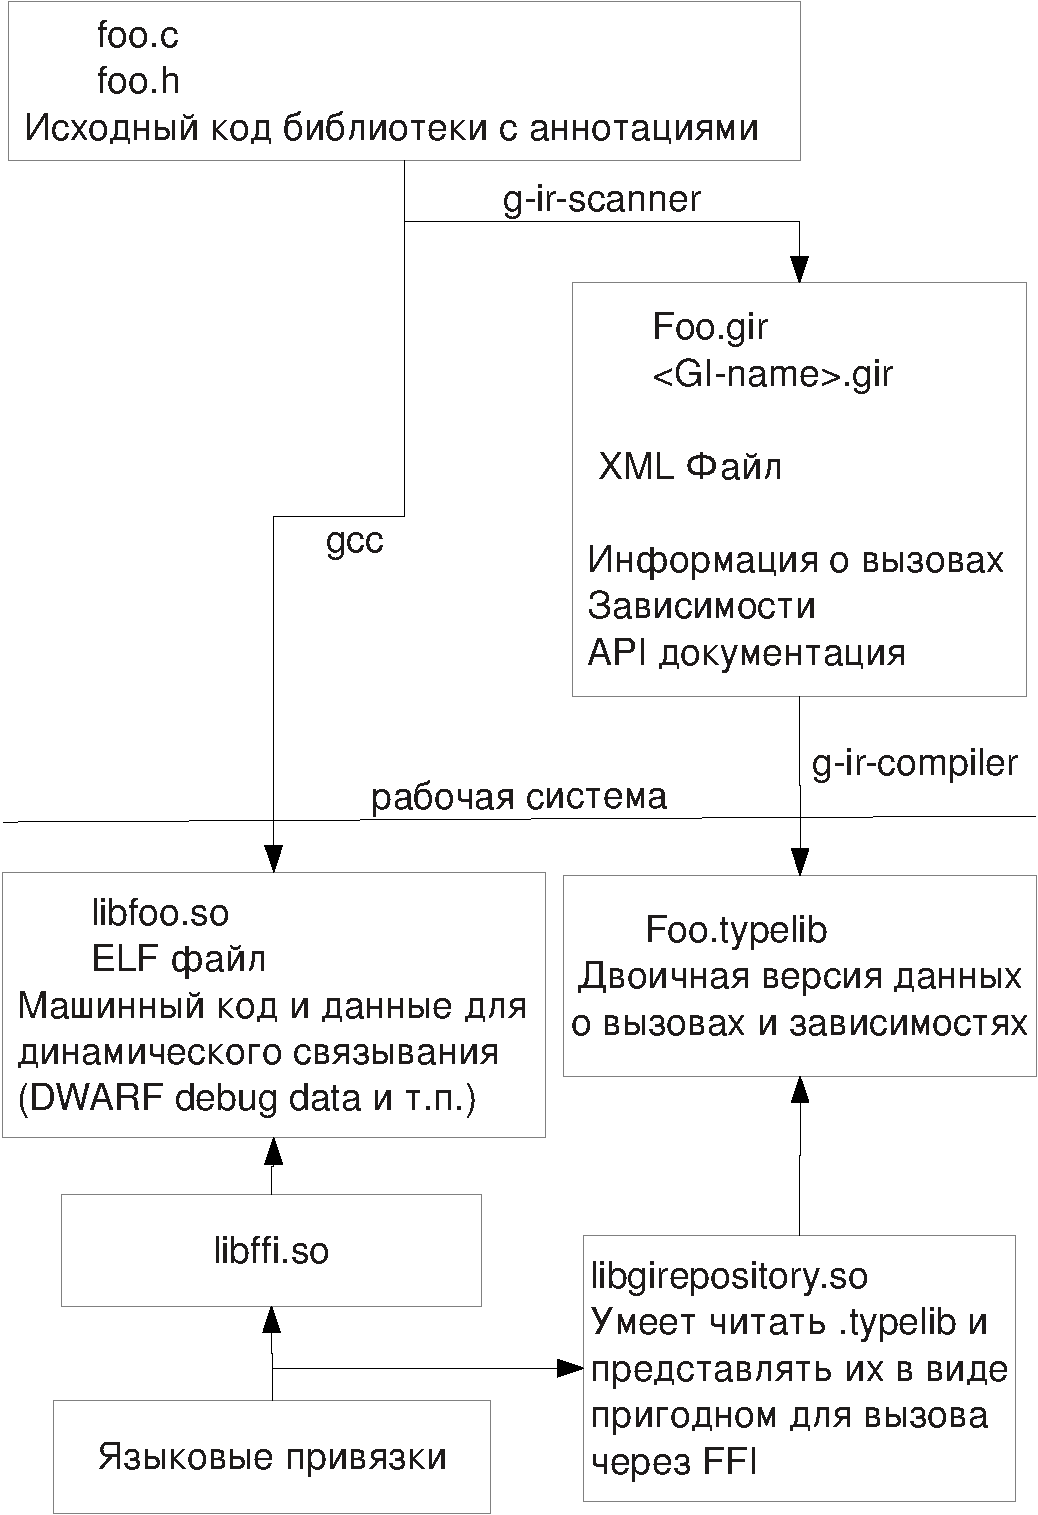
\includegraphics[width=10cm]{103_2012_antono-crop}
  \label{fig:Antono1}
\end{figure}

\subsection*{Примеры использования}

Я создал репозиторий \cite{Antono2} с примерами использования библиотеки,
базирующейся на GObject, через автоматические привязки для разных языков.

Рассмотрим пример, использующий язык Vala для создания библиотеки и
обращения к этой библиотеке из Ruby:

\begin{verbatim}
namespace ValaObject {
	public void say_hello_to(string lang)
	{
		print(@"I love You, $lang!!!\n");
		print("-- Vala\n\n");
	}

	public class ValaClass : Object {
		public string name = "Vala Class";

		public string append_to_name(string suffix) {
			return "%s %s".printf(name, suffix);
		}
	}
}
\end{verbatim}

Ruby использует метаданные из GIR через библиотеку gir\_ffi:

\begin{verbatim}
require 'gir_ffi'

GirFFI.setup(:ValaObject) # Создание объекта

ValaObject.say_hello_to('Ruby')

class MyValaClass < ValaObject::ValaClass
  def append_to_name(suffix)
    super + ' (subclassed) ' + suffix
  end
end

instance = MyValaClass.new
puts instance.append_to_name("called from Ruby")
\end{verbatim}

\subsection*{Существующие привязки}

Список существующих привязок для GObject Introspection выглядит следующим образом:

\begin{itemize}
  \item \url{https://live.gnome.org/Vala}{Vala} "--- Родная поддержка GIR.
  \item \url{https://live.gnome.org/Genie}{Genie} "--- Родная подержка GIR.
  \item \url{https://live.gnome.org/PyGObject}{PyGObject} "--- привязки для Python
  \item \url{https://live.gnome.org/Gjs}{Gjs} "--- Javascript (spidermonkey)
  \item \url{https://live.gnome.org/Seed}{Seed} "--- Javascript (JSCore, WebKit JS engine)
  \item \url{https://github.com/creationix/node-gir}{node-gir} "--- Node.js (V8 Engine)
  \item \url{https://github.com/mvz/ruby-gir-ffi/wiki}{ruby-gir-ffi} "--- Ruby
  \item \url{https://github.com/indeyets/gobject-for-php}{gobject-for-php} "--- PHP
  \item \url{http://oproj.tuxfamily.org/wiki/doku.php?id=lgob}{lgob} "--- Lua (этап компиляции)
  \item \url{https://github.com/pavouk/lgi}{lgi} "--- Lua (этап исполнения)
  \item \url{https://live.gnome.org/GTK2-Perl/Introspection}{GTK2-Perl/Introspection} "--- привязки для Perl
  \item \url{http://gitorious.org/guile-gir}{guile-gir} "--- Scheme (guile)
  \item \url{http://live.gnome.org/sbank}{sbank} "--- Scheme (Ikarus, Ypsilon)
  \item \url{https://live.gnome.org/JGIR}{JGIR} "--- Java/JVM (этап компиляции, через typelib)
  \item \url{https://live.gnome.org/GObjectIntrospection/GObjectConsume}{GObjectIntrospection/GObjectConsume} "--- C++, Qt (этап компиляции)
  \item \url{https://github.com/ex-rzr/factor-gir}{factor-gir} "--- Factor
  \item \url{https://github.com/indeyets/gobject-for-php}{gogobject} "--- Go (этап компиляции)
  \item \url{https://github.com/andy128k/cl-gobject-introspection}{cl-gobject-introspection} "--- Common Lisp
  \item \url{http://bazaar.launchpad.net/~scymtym/+junk/cl-gir/files}{cl-gir} "--- GIR for Common Lisp (в процессе)
  \item \url{http://www.haskell.org/haskellwiki/GObjectIntrospection}{haskel-gi} "--- Haskell (в процессе)
  \item \url{https://github.com/alanmcgovern/mono-introspect}{mono-introspect} "--- Mono
  \item \url{http://git.ocamlcore.org/cgi-bin/gitweb.cgi?p=ocaml-gir/ocaml-gir.git}{ocaml-gir} "--- Ocaml (этап компиляции)
  \item \url{http://wiki.freepascal.org/gir2pascal}{gir2pascal} "--- Pascal
\end{itemize}



\begin{thebibliography}{9}

\bibitem{Antono1} GTK+ Language Bindings. \url{http://www.gtk.org/language-bindings.php}

\bibitem{Antono2} GObject for your favorite language. \url{https://github.com/antono/vala-object}

\end{thebibliography}

\end{document}





\documentclass[10pt, a5paper]{article}
\usepackage{pdfpages}
\usepackage{parallel}
\usepackage[T2A]{fontenc}
\usepackage{ucs}
\usepackage[utf8x]{inputenc}
\usepackage[polish,english,russian]{babel}
\usepackage{hyperref}
\usepackage{rotating}
\usepackage[inner=2cm,top=1.8cm,outer=2cm,bottom=2.3cm,nohead]{geometry}
\usepackage{listings}
\usepackage{graphicx}
\usepackage{wrapfig}
\usepackage{longtable}
\usepackage{indentfirst}
\usepackage{array}
\newcolumntype{P}[1]{>{\raggedright\arraybackslash}p{#1}}
\frenchspacing
\usepackage{fixltx2e} %text sub- and superscripts
\usepackage{icomma} % коскі ў матэматычным рэжыме
\PreloadUnicodePage{4}

\newcommand{\longpage}{\enlargethispage{\baselineskip}}
\newcommand{\shortpage}{\enlargethispage{-\baselineskip}}

\def\switchlang#1{\expandafter\csname switchlang#1\endcsname}
\def\switchlangbe{
\let\saverefname=\refname%
\def\refname{Літаратура}%
\def\figurename{Іл.}%
}
\def\switchlangen{
\let\saverefname=\refname%
\def\refname{References}%
\def\figurename{Fig.}%
}
\def\switchlangru{
\let\saverefname=\refname%
\let\savefigurename=\figurename%
\def\refname{Литература}%
\def\figurename{Рис.}%
}

\hyphenation{admi-ni-stra-tive}
\hyphenation{ex-pe-ri-ence}
\hyphenation{fle-xi-bi-li-ty}
\hyphenation{Py-thon}
\hyphenation{ma-the-ma-ti-cal}
\hyphenation{re-ported}
\hyphenation{imp-le-menta-tions}
\hyphenation{pro-vides}
\hyphenation{en-gi-neering}
\hyphenation{com-pa-ti-bi-li-ty}
\hyphenation{im-pos-sible}
\hyphenation{desk-top}
\hyphenation{elec-tro-nic}
\hyphenation{com-pa-ny}
\hyphenation{de-ve-lop-ment}
\hyphenation{de-ve-loping}
\hyphenation{de-ve-lop}
\hyphenation{da-ta-ba-se}
\hyphenation{plat-forms}
\hyphenation{or-ga-ni-za-tion}
\hyphenation{pro-gramming}
\hyphenation{in-stru-ments}
\hyphenation{Li-nux}
\hyphenation{sour-ce}
\hyphenation{en-vi-ron-ment}
\hyphenation{Te-le-pathy}
\hyphenation{Li-nux-ov-ka}
\hyphenation{Open-BSD}
\hyphenation{Free-BSD}
\hyphenation{men-ti-on-ed}
\hyphenation{app-li-ca-tion}

\def\progref!#1!{\texttt{#1}}
\renewcommand{\arraystretch}{2} %Іначай формулы ў матрыцы зліпаюцца з лініямі
\usepackage{array}

\def\interview #1 (#2), #3, #4, #5\par{

\section[#1, #3, #4]{#1 -- #3, #4}
\def\qname{LVEE}
\def\aname{#1}
\def\q ##1\par{{\noindent \bf \qname: ##1 }\par}
\def\a{{\noindent \bf \aname: } \def\qname{L}\def\aname{#2}}
}

\def\interview* #1 (#2), #3, #4, #5\par{

\section*{#1\\{\small\rm #3, #4. #5}}

\def\qname{LVEE}
\def\aname{#1}
\def\q ##1\par{{\noindent \bf \qname: ##1 }\par}
\def\a{{\noindent \bf \aname: } \def\qname{L}\def\aname{#2}}
}


\begin{document}

\title{Managing over 9000 nodes with Puppet}%\footnote{Текст данных и последующих тезисов, кроме специально оговоренных случаев, доступен под лицензией Creative Commons Attribution-ShareAlike 3.0}

\author{Василий Михаленя\footnote{Минск, Беларусь}}
\maketitle

\begin{abstract}
Puppet is an open source tool to manage configurations. The article describes its features, advantages, scalability, common and best practices. <<SSH in a for loop is not a solution>>, says Luke Kanies, Puppet developer.
\end{abstract}

\section*{Что такое puppet}

Puppet "--- клиент"=серверное приложение для удобного \linebreak распространения конфигураций "--- состоит из puppetmaster'а, сервера хранящего конфигурации, и puppet agent'а, работающего на конфигурируемом сервере. Puppet написан на ruby, распространяется под лицензией Apache и содержит возможности расширения функциональности с использованием ruby. Проект имеет ruby в качестве единственной зависимости, работает на Linux, Solaris, BSD, Mac OS X, поддерживает Microsoft Windows. Puppet можно использовать как для документирования конфигурации на одном сервере, так и для легкого управления конфигурацией парка серверов в гетерогенной среде. Puppet используют такие проекты как wikimedia, twitter, digg, sugarcrm и многие другие.

\section*{Основные примитивы. Puppet или bash}

Описание конфигураций происходит на своем собственном декларативном языке. Декларативный язык позволяет описать желаемое состояние системы в зависимости от набора фактов "--- описание <<как именно делать>>, как правило, не требуется. Если применять некоторую конфигурацию на серверах с разными ОС (или, например, разными дистрибутивами Linux), используя bash скриптинг, получаем трудноподдерживаемый код. Puppet же позволяет быть уверенным не только в том, что изменения были применены единоразово ( случай shell"=сценариев), но и что текущее состояние соответствует описанному. Простота языка позволяет использовать манифесты puppet как документацию конфигурации систем.

К числу основных понятий языка относятся следующие:

\begin{itemize}
  \item ресурсы "--- file, package, user, exec, cron и т.д.
  \item классы "--- объединения ресурсов и зависимости между ними
  \item модули "--- самостоятельные наборы классов, например, для\linebreak конфигурации определенного сервиса. Модули независимы и могут распространяться отдельно.
  \item факты "--- facts "--- пары <<ключ"=значение>>, которыми оперирует puppet для выбора конфигурации (например, hostname =\textgreater{} mars, is\_virtual =\textgreater{} false, operatingsystem =\textgreater{} Ubuntu, \linebreak processorcount =\textgreater{} 8).
  \item ноды "--- nodes "--- соответствие имени сервера (ноды) и набора классов, которые будут к ней применены. Возможно хранение нод в LDAP или использование внешнего классификатора нод "--- произвольного скрипта.
  \item манифест "--- конфигурационный файл puppet, в котором описаны ресурсы, классы, модули или ноды
\end{itemize}

\section*{Управление парком машин от 2 до бесконечности}

Очевидно, что преимуществ от автоматизации применения конфигурации тем больше, чем больше систем и сервисов на них настраиваются с помощью puppet. Но некоторые вещи полезно автоматизировать, если имеются хотя бы 2 ноды:

\begin{itemize}
  \item синхронизация authorized\_keys
  \item синхронизация пользователей, их настроек (bashrc, vimrc \ldots{})
  \item синхронизация правил брандмауэра
  \item и т.д.
\end{itemize}

В гетерогенной среде приходится учитывать <<факты>> в своих конфигурациях. Деплоймент новой или вышедшей из строя ноды происходит в течение нескольких минут при достаточной степени полноты описания конфигурации. Существует огромное количество написанных модулей для практически любых сервисов (их список можно получить поиском, например, на github). Деплоймент или применение каких"=либо изменений для 2 или 2000 нод практически не отличаются по трудоемкости при грамотном подходе.

\section*{Как работает puppet}

Puppet agent раз в 30 минут запрашивает конфигурацию \linebreak у puppetmaster:

\begin{enumerate}
  \item Компиляция манифеста происходит на сервере, результатом являются <<базовые хеши>> и никакой валидации данных.
  \item Инстанциирование "--- конвертация <<базовых хешей>> и массивов, полученных при компиляции, в объекты puppet"=библиотеки. Валидация входных данных происходит на этом этапе.
  \item Конфигурирование "--- сравнение каждого описанного ресурса с реальным положением дел, и внесение соответствующих изменений при необходимости.
\end{enumerate}

Также существует подход nodeless (masterless). При данном подходе, манифеста с описанием нод не существет "--- мастер не нужен, вся конфигурация копируется на ноду, а настройка опирается исключительно на <<факты>>.

\section*{Как масштабировать puppet}

До 100 нод со стандартным периодом в 30 минут могут успешно работать с единственным puppetmaster"=сервером (WEBRick Ruby"=based HTTP). Дальше начинаются проблемы. Выход -- связка mod\_passenger + apache + rack. При данной схеме возможно распределение нагрузки на несколько серверов. Часто используют подход со splay time "--- размазывание по времени нагрузки на мастер "--- при котором все ноды не должны обращаться к мастеру одновременно. Можно также использовать подход 1 мастер на площадку (сайт), с синхронизацией между площадками, например, через тот же git.

\section*{Опыт работы в команде}

Опыт работы с puppet подсказывает следующие практики:

\begin{itemize}
  \item Использование environments, различных наборов манифестов для разработки и продакшна, когда выбор environment происходит на стороне клиента.
  \item Использование системы контроля версий "--- например, git. \linebreakУдобным оказывается использование двух различных веток или репозиториев, для разработки и production соответсвенно.
\end{itemize}



\end{document}





%\documentclass[10pt, a5paper]{article}
\usepackage{pdfpages}
\usepackage{parallel}
\usepackage[T2A]{fontenc}
\usepackage{ucs}
\usepackage[utf8x]{inputenc}
\usepackage[polish,english,russian]{babel}
\usepackage{hyperref}
\usepackage{rotating}
\usepackage[inner=2cm,top=1.8cm,outer=2cm,bottom=2.3cm,nohead]{geometry}
\usepackage{listings}
\usepackage{graphicx}
\usepackage{wrapfig}
\usepackage{longtable}
\usepackage{indentfirst}
\usepackage{array}
\newcolumntype{P}[1]{>{\raggedright\arraybackslash}p{#1}}
\frenchspacing
\usepackage{fixltx2e} %text sub- and superscripts
\usepackage{icomma} % коскі ў матэматычным рэжыме
\PreloadUnicodePage{4}

\newcommand{\longpage}{\enlargethispage{\baselineskip}}
\newcommand{\shortpage}{\enlargethispage{-\baselineskip}}

\def\switchlang#1{\expandafter\csname switchlang#1\endcsname}
\def\switchlangbe{
\let\saverefname=\refname%
\def\refname{Літаратура}%
\def\figurename{Іл.}%
}
\def\switchlangen{
\let\saverefname=\refname%
\def\refname{References}%
\def\figurename{Fig.}%
}
\def\switchlangru{
\let\saverefname=\refname%
\let\savefigurename=\figurename%
\def\refname{Литература}%
\def\figurename{Рис.}%
}

\hyphenation{admi-ni-stra-tive}
\hyphenation{ex-pe-ri-ence}
\hyphenation{fle-xi-bi-li-ty}
\hyphenation{Py-thon}
\hyphenation{ma-the-ma-ti-cal}
\hyphenation{re-ported}
\hyphenation{imp-le-menta-tions}
\hyphenation{pro-vides}
\hyphenation{en-gi-neering}
\hyphenation{com-pa-ti-bi-li-ty}
\hyphenation{im-pos-sible}
\hyphenation{desk-top}
\hyphenation{elec-tro-nic}
\hyphenation{com-pa-ny}
\hyphenation{de-ve-lop-ment}
\hyphenation{de-ve-loping}
\hyphenation{de-ve-lop}
\hyphenation{da-ta-ba-se}
\hyphenation{plat-forms}
\hyphenation{or-ga-ni-za-tion}
\hyphenation{pro-gramming}
\hyphenation{in-stru-ments}
\hyphenation{Li-nux}
\hyphenation{sour-ce}
\hyphenation{en-vi-ron-ment}
\hyphenation{Te-le-pathy}
\hyphenation{Li-nux-ov-ka}
\hyphenation{Open-BSD}
\hyphenation{Free-BSD}
\hyphenation{men-ti-on-ed}
\hyphenation{app-li-ca-tion}

\def\progref!#1!{\texttt{#1}}
\renewcommand{\arraystretch}{2} %Іначай формулы ў матрыцы зліпаюцца з лініямі
\usepackage{array}

\def\interview #1 (#2), #3, #4, #5\par{

\section[#1, #3, #4]{#1 -- #3, #4}
\def\qname{LVEE}
\def\aname{#1}
\def\q ##1\par{{\noindent \bf \qname: ##1 }\par}
\def\a{{\noindent \bf \aname: } \def\qname{L}\def\aname{#2}}
}

\def\interview* #1 (#2), #3, #4, #5\par{

\section*{#1\\{\small\rm #3, #4. #5}}

\def\qname{LVEE}
\def\aname{#1}
\def\q ##1\par{{\noindent \bf \qname: ##1 }\par}
\def\a{{\noindent \bf \aname: } \def\qname{L}\def\aname{#2}}
}


\begin{document}
\renewcommand{\figurename}{Рыс.} % Не перакідаць у прэамбулу --- не працуе, чаму -- халера ведае.
\renewcommand{\abstractname}{Анатацыя}
\renewcommand{\refname}{Літаратура}

\title{Выкарыстанне свабоднага праграмнага забеспячэння ва ўстановах адукацыі Украіны: спроба аналізу}

\author{Грыгорый Злобiн\footnote{Львоўскі нацыянальны ўніверсітэт ім. Івана Франка, \url{zlobin@electronics.wups.lviv.ua}}}
\date{}

\maketitle

\begin{abstract}
The analysis of free / open source software usage in higher educational institutions of Ukraine is presented, based of the `FOSS Lviv-2011'  International Scientific Conference reports. 
\end{abstract}

Нягледзячы на станоўчы досвед выкарыстання свабодных праграм у адукацыі як у краінах блізкага, так і далёкага замежжа, ва Украіне да гэтага часу не прынятая канцэпцыя выкарыстання свабоднага праграмнага забеспячэння у адукацыі. Разам з тым намаганнямі энтузіястаў у навучальных установах Украіны свабоднае праграмнае забеспячэнне ўсё ж выкарыстоўваецца! Праз адасобленую пазіцыю Міністэрства адукацыі і навукі Украіны няма падрабязнай інфармацыі аб досведзе выкарыстання свабодных праграм у адукацыі. Дзякуючы таму, што ў Львоўскім нацыянальным універсітэце імя Івана Франка 01--06 лютага 2011 адбылася даволі прадстаўнічая міжнародная навукова"=практычная канферэнцыя <<FOSS Lviv-2011>>, з'явілася магчымасць правядзення аналізу выкарыстання СПЗ у вышэйшых навучальных установах Украіны. З 81 дакладаў 49 было прысвечана выкарыстанню СПЗ у навучальных установах. Даклады \cite{fosslviv}, якія былі пададзеныя на гэтую канферэнцыю, можна згрупаваць па наступных кірунках (назва дакладу падаецца на мове арыгіналу):

\section*{Дыстанцыйнае навучанне}
Гэтай тэматыцы прысвечаная найбольшая колькасць дакладаў "--- 10:
\begin{itemize}
\item <<Розроблення електронного деканату для системи управління дистанційним навчання MOODLE>> --- Артеменко В.Б., Львоўская камерцыйная акадэмія
\item <<Вибір платформи дистанційного навчання>> --- Коцаренко М.В., Бойко О.В.,  Львоўскі нацыянальны медыцынскі ўніверсітэт ім. Данііла Галіцкага
\item <<Використання контрольно-діагностичної програми iTest у ході моніторингу якості процесу навчання старшокласників>> --- Макаренко І.Є., Мерзлікін П.В., Крыварожскі дзяржаўны педагагічны ўніверсітэт
\item  <<Використання системи Moodle для організації контролю знань майбутніми вчителями-гуманітаріями>> --- Маркова Є.С., Бердзянскі дзяржаўны педагагічны ўніверсітэт
\item  <<Тестування в  Moodle як елемент менеджменту якості освіти: перший досвід>> --- Сергієнко В.П., Сліпухіна І.А., НПУ ім. М.П. Драгаманава
\item  <<Особливості програмного забезпечення в електронному навчанні>> --- Жарких Ю.С., Лисоченко С.В., Сусь Б.Б., Третяк О.В., Кіеўскі нацыянальны ўніверсітэт ім. Тараса Шаўчэнкі
\item  <<Інформаційно-аналітична система управління навчальним процесом ВНЗ на базі  Moodle>> --- Триус Ю.В., Чаркаскі дзяржаўны тэхналагічны ўніверсітэт
\item  <<Використання CMS JOMLA!  та LCMS MOODLE у ВНЗ>> --- Франчук В.М., НПУ ім. М.П. Драгаманава
\item <<Локалізація системи MOODLE " --- Франчук В.М., НПУ ім. М.П. Драгаманава
\item  <<Застосування вільного програмного забезпечення для дистанційного навчання у вищих навчальних закладах>> --- Захарченко В.М., Шапо В.М., Адэская нацыянальная марская акадэмія
\end{itemize}
\newpage

\section*{Выкарыстанне сістэм кампутарнай матэматыкі}
Наступныя 6 дакладаў можна аднесці да матэматычнай тэматыкі:
\begin{itemize}
\item <<Використання вільно-поширюваного ПЗ математичного призначення в університеті>> "--- Бугаєць Н.О., НПУ ім. М.П. Драгаманава
\item <<Вільнопоширювані системи комп'ютерної математики в осві\-ті і науці>> "--- Лазурчак І.І., Кобильник Т.П., Драгобыцкі дзяржаўны ўніверсітэт ім. І. Франка
\item <<Використання комп'ютерних математичних систем у про\-фе\-сій\-ній підготовці майбутнього вчителя математики>> "--- Лов'я\-но\-ва І.В., Крыварожскі дзяржаўны педагагічны ўніверсітэт
\item <<Моделювання задач електротехніки у XCOS>> "--- Філь І.М., Данецкі нацыянальны тэхнічны ўніверсітэт
\item <<Розробка і використання web-інтерфейсів для роботи з системами комп'ютерної математики>> "--- Чичкарьов Є.А., Прыазоўскі дзяржаўны тэхнічны ўніверсітэт
\item <<Про комп'ютерний супровід викладання геометрії>> "--- Яхненко І.В., Лутфулін М.В., Палтаўскі нацыянальны педагагічны ўніверсітэт ім. В.Г. Караленкі
\end{itemize}

\section*{Агульныя пытанні выкарыстання СПЗ у адукацыі}
7 дакладаў гэтай групы, якую можна прызнаць другой па колькасці, уключалі:
\begin{itemize}
\item <<Використання вільного програмного забезпечення в навчанні і наукових дослідженнях у Львівському національному уні\-вер\-ситеті імені Івана Франка>> "--- Апуневич С.Є., Злобін Г.Г., Рикалюк Р.Є., Шувар Р.Я., Львоўскі нацыянальны ўніверсітэт ім. І. Франка
\item <<Використання вільного програмного забезпечення в системі дистанційної освіти>> "--- Воронкін О.С., Луганскі дзяржаўны інстытут культуры і мастацтваў
\item <<Вільнопоширюване програмне забезпечення курсу “Нові інформаційні технології” для студентів спеціальності \linebreak “Біо\-ло\-гія”>> "--- Єфименко В.В., НПУ ім. М.П. Драгаманава
\item <<Використання вільного програмного забез\-печення у про\-фе\-сій\-ній підготовці майбутніх інженерів>> "--- Покришень Д.А., \linebreak Дрозд О.П., Сподаренко І.Й., Чарнігаўскі дзяржаўны тэхналагічны ўніверсітэт
\item  <<Про досвід використання ОС Linux у навчальному процесі Львівського національного медичного університету імені Данила Галицького>> "--- Риковський П.А., Львоўскі нацыянальны медыцынскі ўніверсітэт ім. Данііла Галіцкага
\item  <<LINUX  та VIRTUAL-BOX у навчанні абстрактних понять теорії операційних систем>> "--- Спірін О.М., Сверчевська О.С., Жытомірскі дзяржаўны ўніверсітэт ім. І. Франка
\item  <<З досвіду використання вільного програмного забезпечення при вивченні інформатики>> "--- Харченко В.М., Нежынскі дзяржаўны ўніверсітэт ім. М. Гогаля
\end{itemize}

\section*{Выкарыстанне адкрытых сродкаў праграмавання}
Гэтая група апынулася найменшай па колькасці і ўключае 4 даклады:
\begin{itemize}
\item <<Використання відкритих програмних засобів в процесі навчання статистичним дисциплінам>> "--- Коркуна Т.Й., Самбарскі тэхнікум эканомікі і інфарматыкі
\item <<Розрахунок фотоіонізаційних моделей небулярного газу в ОС LINUX UBUNTU 10.10 та WINDOWS 7>> "--- Мелех Б.Я., Тишко Н.Л., Коритко Р.І., Львоўскі нацыянальны ўніверсітэт ім. І. Франка
\item <<Реалізація розподілених обчислень на основі грід-платформи з відкритим кодом BOINC>> "--- Шийка Ю.Я., Шувар Р.Я., \linebreak Львоўскі нацыянальны ўніверсітэт ім. І. Франка
\item <<Реалізація високопродуктивної обчислювальної системи на базі ОС  LINUX>> "--- Шувар Р.Я., Бойко Я.В., Львоўскі нацыянальны ўніверсітэт ім. І. Франка
\end{itemize}

\section*{Распрацоўка праграмнага забеспячэння}
Будучы тэматычна-роднаснай папярэдняй, гэтая група больш шматлікая і складаецца з 7 дакладаў, яна зраўнавалася з катэгорыяй <<Агульныя пытанні выкарыстання СПЗ у адукацыі>>:
\begin{itemize}
\item <<Комплекс програм для лазерних спостережень штучних супутників Землі>> "--- Мартинюк-Лотоцький К.П., Білінський\linebreak А.\,І., Львоўскі нацыянальны ўніверсітэт ім. І. Франка
\item <<Розробка системи спектральної діагностики димової плазми>> "--- Сподарець Д.В., Драган Г.С., Адэскі нацыянальны ўні\-версітэт імя І.І. Мечнікава
\item <<Використання вільного програмного забез-печення для створення програми керування інформаційним автоматом>> "--- Зло\-бін Г., Скляр В., Чмихало О., Шевчик В., Львоўскі нацыянальны ўніверсітэт ім. І. Франка
\item <<Використання бібліотеки класів GEANT4 в ОС Linux при розробці програмного забезпечення для моделювання процесів взаємодії випромінювання з речовиною>> "--- Малихіна Т.В., Харкаўскі нацыянальны ўніверсітэт ім. В.Н. Каразіна
\item  <<Програма для обробкирезультатів ЛЛС-спостережень як \linebreak ВПЗ>> "--- Апуневич С.Є., Апуневич С.В., Білінський А.І., Благодир Я.Т., Львоўскі нацыянальны ўніверсітэт ім. І. Франка
\item  <<Програмне забезпечення керування телескопом  ЛЛС-станції Львів-1831>> "--- Білінський А.І., Мартинюк-Лотоцький К.\,П., \linebreak Львоўскі нацыянальны ўніверсітэт ім. І. Франка
\item <<Використання Open Wrt як основи вбудованого програмного забезпечення маршрутизаторів>> "--- Нек Т., Львоўскі нацыянальны ўніверсітэт ім. І. Франка
\end{itemize}

\section*{Асобныя даклады}
І нарэшце, 5 дакладаў немагчыма аднесці ні да адной з пералічаных вышэй катэгорый:
\begin{itemize}
\item  <<Інформаційна технологія управління навчальним навантаженням у вищих навчальних закладах>> "--- Гриценко В.Г., Чаркаскі нацыянальны ўніверсітэт ім. Б. Хмяльніцкага
\item  <<Про досвід використання офісного  пакету OpenOffice.org.ukr в курсі інформатики для економічних і юридичних спеціальностей ВЗО>> "--- Злобін Г.Г., Львоўскі нацыянальны ўніверсітэт ім. І. Франка 
\item  <<Досвід використання  редактора Gimp при вивченні курсу “Комп'ютерна графіка і дизайн”>> "--- Матвієнко Ю.С., Палтаўскі нацыянальны педагагічны ўніверсітэт ім. В.Г. Караленкі
\item <<Використання програми GANTTPROJECT для побудови календарних графіків при розробці ПВР>> "--- Грицук Ю.В., Меліхов О.І., Данбаская акадэмія будаўніцтва і архітэктуры
\item <<Вільне ПЗ для підготовки наукових текстів і презентацій>> "--- Лутфуллін М.В., Моторний М.І., Палтаўскі нацыянальны педагагічны ўніверсітэт ім. В.Г. Караленкі
\end{itemize}

	Такім чынам, можна канстатаваць як шырокі спектр выкарыстання СПЗ ва ўкраінскіх навучальных установах ад дыстанцыйнага навучання да распрацоўкі адкрытага праграмнага забеспячэння, так і шырокую геаграфію выкарыстання СПЗ ад Луганска на ўсходзе да Львова на захадзе і ад Чарнігава на поўначы да Адэсы на поўдні (глядзі рыс.).

\begin{figure}[ht]
\centering{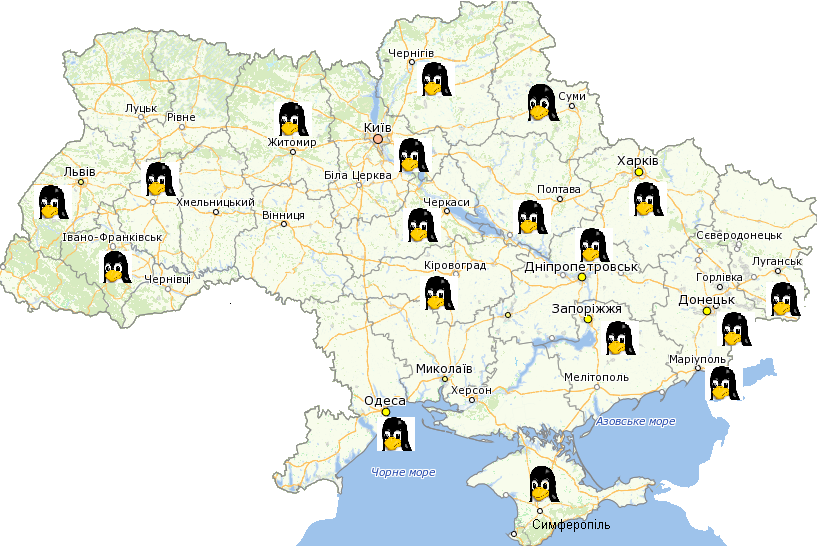
\includegraphics[width=8cm]{05_ukraine_linux.png}}
\label{pic:fl1}
%\caption{~}
\end{figure}

\begin{thebibliography}{9}
\bibitem{fosslviv}Тези міжнародної науково-практичної конференції FOSS LVIV-2011. Збірник наукових праць /за ред. Злобіна Г.Г., Апуневича С.Є., Машкова В.В., Апуневич С.В. Вид-во ЛНУ імені Івана Франка. 2011. --- 196 с.
\end{thebibliography}

\end{document}





%\documentclass[a5paper,10pt]{article}
\usepackage{pdfpages}
\usepackage{parallel}
\usepackage[T2A]{fontenc}
\usepackage{ucs}
\usepackage[utf8x]{inputenc}
\usepackage[polish,english,russian]{babel}
\usepackage{hyperref}
\usepackage{rotating}
\usepackage[inner=2cm,top=1.8cm,outer=2cm,bottom=2.3cm,nohead]{geometry}
\usepackage{listings}
\usepackage{graphicx}
\usepackage{wrapfig}
\usepackage{longtable}
\usepackage{indentfirst}
\usepackage{array}
\newcolumntype{P}[1]{>{\raggedright\arraybackslash}p{#1}}
\frenchspacing
\usepackage{fixltx2e} %text sub- and superscripts
\usepackage{icomma} % коскі ў матэматычным рэжыме
\PreloadUnicodePage{4}

\newcommand{\longpage}{\enlargethispage{\baselineskip}}
\newcommand{\shortpage}{\enlargethispage{-\baselineskip}}

\def\switchlang#1{\expandafter\csname switchlang#1\endcsname}
\def\switchlangbe{
\let\saverefname=\refname%
\def\refname{Літаратура}%
\def\figurename{Іл.}%
}
\def\switchlangen{
\let\saverefname=\refname%
\def\refname{References}%
\def\figurename{Fig.}%
}
\def\switchlangru{
\let\saverefname=\refname%
\let\savefigurename=\figurename%
\def\refname{Литература}%
\def\figurename{Рис.}%
}

\hyphenation{admi-ni-stra-tive}
\hyphenation{ex-pe-ri-ence}
\hyphenation{fle-xi-bi-li-ty}
\hyphenation{Py-thon}
\hyphenation{ma-the-ma-ti-cal}
\hyphenation{re-ported}
\hyphenation{imp-le-menta-tions}
\hyphenation{pro-vides}
\hyphenation{en-gi-neering}
\hyphenation{com-pa-ti-bi-li-ty}
\hyphenation{im-pos-sible}
\hyphenation{desk-top}
\hyphenation{elec-tro-nic}
\hyphenation{com-pa-ny}
\hyphenation{de-ve-lop-ment}
\hyphenation{de-ve-loping}
\hyphenation{de-ve-lop}
\hyphenation{da-ta-ba-se}
\hyphenation{plat-forms}
\hyphenation{or-ga-ni-za-tion}
\hyphenation{pro-gramming}
\hyphenation{in-stru-ments}
\hyphenation{Li-nux}
\hyphenation{sour-ce}
\hyphenation{en-vi-ron-ment}
\hyphenation{Te-le-pathy}
\hyphenation{Li-nux-ov-ka}
\hyphenation{Open-BSD}
\hyphenation{Free-BSD}
\hyphenation{men-ti-on-ed}
\hyphenation{app-li-ca-tion}

\def\progref!#1!{\texttt{#1}}
\renewcommand{\arraystretch}{2} %Іначай формулы ў матрыцы зліпаюцца з лініямі
\usepackage{array}

\def\interview #1 (#2), #3, #4, #5\par{

\section[#1, #3, #4]{#1 -- #3, #4}
\def\qname{LVEE}
\def\aname{#1}
\def\q ##1\par{{\noindent \bf \qname: ##1 }\par}
\def\a{{\noindent \bf \aname: } \def\qname{L}\def\aname{#2}}
}

\def\interview* #1 (#2), #3, #4, #5\par{

\section*{#1\\{\small\rm #3, #4. #5}}

\def\qname{LVEE}
\def\aname{#1}
\def\q ##1\par{{\noindent \bf \qname: ##1 }\par}
\def\a{{\noindent \bf \aname: } \def\qname{L}\def\aname{#2}}
}


\begin{document}


\title{Облачные вычисления и сервисы: классификация, основные функции, преимущества и недостатки}

\author{Виталий Сороко\footnote{Минск, \url{http://arneta.ru}}}

\maketitle
\begin{abstract}
In the past, big part of computer-related activity was impos\-sible without the installation of software to a local computer, but now, with help of cloud services, users can perform such typical tasks as word processing within their web-browser. It becomes possible due to so called cloud-based resources. Here an attempt of  cloud technologies and systems general overview is presented with the technical description of the architecture, characteristics and features comparison. 
\end{abstract}

Среди наиболее полных определений облачных систем на сегодняшний день можно выделить следующие два:
\begin{itemize}
\item Облачные сервисы "--- это технология обработки данных, в которой программное обеспечение предоставляется пользователю как интернет-сервис, при котором от пользователя скрыта инфраструктура <<облака>> (облачной системы) и, поэтому, ему не требуются специальные знания и навыки для  управления и использования данной <<облачной>> технологии.
\item Облачные вычисления "--- это вычисления, которые представляют собой динамически масштабируемый способ доступа к внешним вычислительным ресурсам в виде сервиса, предоставляемого посредством Интернета.
\end{itemize}

Данные определения тесно связаны между собой: для реализации всех облачных сервисов необходимы вычисления, а облачные вычисления по сути сами являются облачным сервисом. Рассмотрим классификацию облачных сервисов и их реализаций из мира свободного ПО.

В настоящее время все облачные сервисы подразделяют на:
\begin{itemize}
\item \emph{«Программное обеспечение как услуга»} (Software as a Service, сокращённо SaaS) "--- бизнес-модель продажи программного \linebreak обеспечения, при которой владелец (поставщик) ПО предоставляет доступ к к нему пользователям (заказчикам) через Интернет. Примерами такого ПО являются Feng Office Community Edition, Simple Groupware, Zarafa и др.
\item \emph{«Оборудование (вычислительные мощности) как услуга»} \linebreak (Hardware as a Service, сокращённо HaaS) "--- предоставление  вычислительных ресурсов оборудования (его процессорного времени, места для место под хранения данных и т.д.) в виде сервисов с использованием технологий виртуализации. Сервисы обычно предлагаются как эквивалент реальным вычислительным системам, таким как серверы, суперкомпьютеры и др. Над программной реализацией этой идеи полностью или частично работают проекты OpenVZ, FreeVPS, Linux-VServer, Apache Hama, GlusterFS Open Source Project, а также Moose File System (MooseFS) и др., а предоставляет такой сервис на базе OpenSource решений компания Linode и некоторые другие.
\item \emph{<<Коммуникация как Сервис>>} (Communications as a Service, сокр. CaaS) "--- построенное в облаке коммуникационное решение для предприятия, которое обеспечивает передачу речевого сигнала по сети Интернет или по любым другим IP-сетям (VoIP), обмен мгновенными сообщениями (IM), видеоконференции. Модель CaaS позволяет деловым клиентам выборочно разворачивать средства коммуникаций и услуг на оснований оплаты услуг в срок для используемых сервисов. С этим направлением тесно связаны такие FOSS-проекты как Ekiga, iLBC, Speex.
\item \emph{«Мониторинг как Сервис»} (Monitoring-as-a-Service, сокращённо MaaS) является обслуживаемым в облаке программным обеспечением для мониторинга и обеспечения безопасности. Такими OpenSource-решениями на сегодняшний день являются Ganglia, Zabbix, Hyperic HQ. Сюда же  с некоторыми оговорками модно отнести и Nagios. 
\item \emph{«Инфраструктура как услуга»} (Infrastructure as a Service, сокращённо IaaS) "--- это предоставление компьютерной инфраструктуры (как правило в форме виртуализации) как услуги на основе концепции облачных вычислений. По сути IaaS является комбинацией SaaS,  HaaS, так как она включает в себя и то и другое, причем обычно во множественном числе, а также CaaS и иногда MaaS с целью объедения и мониторинга всей системы, и, поэтому, используется в основном предприятиями. Свободными реализациями данной концепции являются Eucalyptus, OpenNebula, OpenStack, Nimbus и др.
\item \emph{«Платформа как услуга»} (Platform as a Service, сокр. PaaS) "--- предоставление программной платформы и инструментов с определенными характеристиками, необходимых для разработки, тестирования, развертывания, поддержки различных приложений. Сюда же входят и готовые к использованию облачные сервисы, которые вместе образуют программную платформу. Яркими примерами из мира OpenSource в настоящее время являются Xen Cloud Platform, Cloud Foundry, Apache Hadoop, Apache Hive и др.
\item \emph{«Компьютер (виртуальный рабочий стол) как услуга»} (Desk\-top as a Service, сокращённо DaaS) "--- предоставление виртуального компьютера, который каждый пользователь может индивидуально настраивать под свои задачи. Таким образом, пользователь приходя на работу просто вводит свои данные (обычно логин и пароль) и может работать, используя при этом благодаря технологиям виртуализации вычислительные мощности стороннего сервера, а не своего ПК. 
\item \emph{<<Рабочее окружение как услуга>>} (Workspace as a Service, сокращённо WaaS) "--- предоставление комплекта  SaaS, предназначенного для создания рабочего окружения. В отличие от DaaS в этом случае пользователь получает доступ только к ПО, в то время как все вычисления происходят непосредственно на его машине. По сути данная категория является гибридом SaaS и PaaS, так как в отличие от последней является платформой, направленной не на разработку и тестирование ПО, а на офисную работу, но при этом как первая в реализации не использует технологий виртуализации. На данный момент реализации данной технологии предоставляются в основном различными крупными компаниями, например Google и Microsoft, и представляют в основном решения с закрытым исходным кодом, иногда с использованием свободных и открытых компонентов или их исходников.
\item \emph{«Все как услуга»} (Everything as a service, сокращённо EaaS) "--- концептуальная модель, включающая в себя элементы всех перечисленных решений. На данный момент полной её реализации не существует "--- она по сути является идеалом для крупных облачных компаний, таких как Google и Microsoft.
\end{itemize}

Свободное и открытое программное обеспечение в настоящее время играет ключевую роль в создании и развертывании облачных сервисов и систем. С одной стороны существуют ряд созданных сообществом платформ, ориентированных на облачные вычисления (Xen, Eucaliptus, Cloud Foundry, Feng Office и др.). С другой стороны, само свободное ПО (операционные системы семейства Linux и BSD, Web-браузеры и т.\,д.) как нельзя лучше подходит для размещения и использования облачных сервисов.  Естественно, что существует и целый ряд проприетарных аналогов.

Рыночная доля облачных сервисов и платформ постоянно растет благодаря ряду преимуществ для обычных пользователей и организаций, среди которых в первую очередь можно отметить:
\begin{itemize}
\item	количество процессоров, объем оперативной памяти и дискового пространства в облачных системах теоретически ничем не ограничен;
\item	пользователям не нужно самостоятельно устанавливать и настраивать ПО, т.\,к. для доступа к облачным сервисам достаточно обычного web-браузера;
\item	пользователям не нужно покупать дорогое оборудование;
\item	экономия времени и энергии на выполнение некоторых задач, а также, в особых случаях, и площадей, занимаемых оборудованием;
\item	возможность производить оплату только за потребленные вычислительные мощности и произведенные операции;
\item	в организациях отсутствуют затраты на развёртывание инфраструктуры;
\item	организации получают сокращение затрат на техническую поддержку и обновление развернутых систем, а также высокую скорость внедрения, обусловленную отсутствием временных затрат на развертывание системы;
\item	отсутствует необходимость обучения "--- большинство пользователей уже умеют пользоваться web-браузерами и интернет-сервисами как классом услуг;
\item	обычно облачные системы обслуживаются высококвалифицированными профессионалами, что дает более высокий уровень качества обслуживания ПО.
\end{itemize}

Тем не менее облачные системы не лишены недостатков, которые в большей степени касаются обычных пользователей, и в меньшей --- провайдеров:
\begin{itemize}
\item из-за вопросов безопасности не все данные можно доверить стороннему провайдеру, тем более, не только для хранения, но и для обработки;
\item далеко не каждое облачное приложение позволяет сохранить полученные результаты в удобном для пользователя виде на нужный носитель данных;
\item риск массовой потери данных многими пользователями из-за технического сбоя у поставщика облачных услуг;
\item потеря свободы "--- большая часть облачных сервисов не имеет четких стандартов, и поэтому при переходе от одного поставщика облачных услуг к другому могут возникнуть серьезные проблемы. Они же могут возникнуть и при обновлении провайдером собственных облачных сервисов "--- если, например, он пожелает внедрить новый интерфейс, то подписчикам придётся им пользоваться.  Немаловажным моментом также является необходимость доступа в интернет, что в некоторых случаях ведет к потере свободы перемещений. А главное, благодаря тому, что все данные находятся в руках провайдера, нельзя исключать того, что недобросовестные компании могут воспользоваться этим.
\end{itemize}

Можно предположить, что как сейчас большая часть пользователей использует Windows и Microsoft Office, так в ближайшем будущем эти пользователи оценят преимущества облачных платформ и перейдут на них. При этом, даже передумав после получения очередной порции счетов за оплату сервисов, пользователям будет трудно вернуться к прежней схеме работы "--- все их данные будут в руках компании"=владельца облачной системы, а для самостоятельной установки другой операционной системы и иного программного обеспечения многим не хватит квалификации, да и приобретённое пользователями оборудование скорее всего будет иметь крайне малую мощность. В этом случае эффективным выходом оказывается  свободное ПО, которое как правило способно работать на маломощном оборудовании при сохранении совместимости со старыми системами. В этом случае возврат пользователей из облака также едва ли станет массовым, поскольку крупные облачные компании постараются сделать этот переход невыгодным, если не невозможным, однако сам факт такой возможности будет являться дополнительным регулирующим фактором, ограничивающим прибыли провайдеров облачных услуг.

\end{document}

%\documentclass[10pt, a5paper]{article}
\usepackage{pdfpages}
\usepackage{parallel}
\usepackage[T2A]{fontenc}
\usepackage{ucs}
\usepackage[utf8x]{inputenc}
\usepackage[polish,english,russian]{babel}
\usepackage{hyperref}
\usepackage{rotating}
\usepackage[inner=2cm,top=1.8cm,outer=2cm,bottom=2.3cm,nohead]{geometry}
\usepackage{listings}
\usepackage{graphicx}
\usepackage{wrapfig}
\usepackage{longtable}
\usepackage{indentfirst}
\usepackage{array}
\newcolumntype{P}[1]{>{\raggedright\arraybackslash}p{#1}}
\frenchspacing
\usepackage{fixltx2e} %text sub- and superscripts
\usepackage{icomma} % коскі ў матэматычным рэжыме
\PreloadUnicodePage{4}

\newcommand{\longpage}{\enlargethispage{\baselineskip}}
\newcommand{\shortpage}{\enlargethispage{-\baselineskip}}

\def\switchlang#1{\expandafter\csname switchlang#1\endcsname}
\def\switchlangbe{
\let\saverefname=\refname%
\def\refname{Літаратура}%
\def\figurename{Іл.}%
}
\def\switchlangen{
\let\saverefname=\refname%
\def\refname{References}%
\def\figurename{Fig.}%
}
\def\switchlangru{
\let\saverefname=\refname%
\let\savefigurename=\figurename%
\def\refname{Литература}%
\def\figurename{Рис.}%
}

\hyphenation{admi-ni-stra-tive}
\hyphenation{ex-pe-ri-ence}
\hyphenation{fle-xi-bi-li-ty}
\hyphenation{Py-thon}
\hyphenation{ma-the-ma-ti-cal}
\hyphenation{re-ported}
\hyphenation{imp-le-menta-tions}
\hyphenation{pro-vides}
\hyphenation{en-gi-neering}
\hyphenation{com-pa-ti-bi-li-ty}
\hyphenation{im-pos-sible}
\hyphenation{desk-top}
\hyphenation{elec-tro-nic}
\hyphenation{com-pa-ny}
\hyphenation{de-ve-lop-ment}
\hyphenation{de-ve-loping}
\hyphenation{de-ve-lop}
\hyphenation{da-ta-ba-se}
\hyphenation{plat-forms}
\hyphenation{or-ga-ni-za-tion}
\hyphenation{pro-gramming}
\hyphenation{in-stru-ments}
\hyphenation{Li-nux}
\hyphenation{sour-ce}
\hyphenation{en-vi-ron-ment}
\hyphenation{Te-le-pathy}
\hyphenation{Li-nux-ov-ka}
\hyphenation{Open-BSD}
\hyphenation{Free-BSD}
\hyphenation{men-ti-on-ed}
\hyphenation{app-li-ca-tion}

\def\progref!#1!{\texttt{#1}}
\renewcommand{\arraystretch}{2} %Іначай формулы ў матрыцы зліпаюцца з лініямі
\usepackage{array}

\def\interview #1 (#2), #3, #4, #5\par{

\section[#1, #3, #4]{#1 -- #3, #4}
\def\qname{LVEE}
\def\aname{#1}
\def\q ##1\par{{\noindent \bf \qname: ##1 }\par}
\def\a{{\noindent \bf \aname: } \def\qname{L}\def\aname{#2}}
}

\def\interview* #1 (#2), #3, #4, #5\par{

\section*{#1\\{\small\rm #3, #4. #5}}

\def\qname{LVEE}
\def\aname{#1}
\def\q ##1\par{{\noindent \bf \qname: ##1 }\par}
\def\a{{\noindent \bf \aname: } \def\qname{L}\def\aname{#2}}
}

\begin{document}
\title{Cистема распределенного выполнения задач paexec }
\author{Алексей Чеусов\\
\small Минск, Беларусь}
\def\progref!#1!{\texttt{#1}}

\maketitle

\begin{abstract}paexec distributes tasks across several CPUs or machines in a
network and collects results from those CPUs/machines. paexec runs
several instances of ``calculator'' on remote/local machines and sends
them tasks one by one recieving results from them. ``tasks'' given on
input may be either a list of independent tasks or a dependency
graph. ``transport'' is any rsh/ssh-like program. Cool features:
resistance to network failures, minimization of total calculation
time.
\end{abstract}

В последнее время все большее распространение получают компьютерные
системы оснащенные большим количеством процессоров или ядер.  В
настоящее время многоядерными процессорами комплектуются не только
мощные сервера и рабочие станции, но также ноутбуки, нетбуки и
даже мобильные телефоны и планшеты. В связи с этим часто возникает
задача распараллеливания выполнения задач с использованием всех
имеющихся вычислительных ресурсов. Та же проблема возникает при
использовании кластера компьютеров, объединенных в вычислительную
сеть. Задача не нова, и для ее решения имеется масса инструментов,
таких, например, как MPI, стандартный API (реализован в библиотеках
openmpi, mpich и др.), широко применяемый математиками для расчетов на
супер-ЭВМ и кластерах.  Тем не менее, существующие инструменты не
лишены недостатков.  В силу лицензионных ограничений далеко не всегда
имеющиеся инструменты можно легально использовать в коммерческих
целях, часто они имеют весьма специфическую область применения и
неудобны для решения простых пользовательских задач, существующие
инструменты порой слишком требовательны к количеству оперативной
памяти и дискового пространства, а то и просто ограничены конкретной
программно-аппаратной архитектурой.

Задача, ставшая в свое время перед автором --- обработка больших
массивов информации, а позднее обработка дерева задач, с
использованием нескольких компьютеров различной аппаратной
архитектуры. При этом <<задача>> в моем случае решалась автономной
программой, написанной с применением различных языков
программирования. Не найдя готового решения, подходящего для моего
случая, я разработал программный пакет paexec с открытым исходным
кодом (лицензия MIT), и разместил его в сети Интернет для публичного
доступа.

Домашняя страница проекта: \url{http://paexec.sf.net/}.

\section*{Как это работает}
В программный пакет paexec входят на данный момент
две программы, главная из которых -- paexec(1), собственно инструмент для
распараллеливания, получающий в качестве аргументов
\begin{enumerate}
\item \emph{задачи} для выполнения. Каждая отдельная задача --- это
   произвольная текстовая строка, не содержащая пробелов. Это может
   быть, например, имя файла, формула для вычисления и
   т.п. Совокупность же задач может представлять собой множество
   независимых задач, то есть задач, которые могут выполняться
   параллельно, либо орграф, узлами в котором являются задачи, а ребро
   $(A, B)$ означает: <<для выполнения задачи $B$ необходимо сначала
   выполнить задачу $A$; если задача $A$ по каким-либо причинам не смогла
   быть выполнена, пометить задачу $B$ и все другие задачи, зависящие от
   A как невыполненные>>. В целях задания порядка выполнения задач,
   каждой их них можно поставить в соответствии некоторый вес,
   определяющий, в какой момент лучше начать ее обработку. Реализовано
   несколько механизмов учета данных весов. В качестве веса можно,
   например, выбрать приблизительное время выполнения задачи или ее
   важность.
\item \emph{список узлов}, на которых, будут производится вычисления, узлами
   могут быть, например, имена компьютеров в сети или номера процессоров,
   адреса chroot пространств на UNIX"=системе и т.д.
\item \emph{вычислитель}. Это программа, принимающая на вход задачу для
   вычисления и печатающая на стандартный поток вывода результаты в
   определенном формате.
\item \emph{транспорт}, задающий способ связи с узлами, им могут быть такие
   программы как rsh, ssh или любые другие с совместимым способом
   использования. В случае, если транспорт не указан, \emph{вычислители}
   будут запущены локально указанное число раз.
\end{enumerate}

На стандартный поток вывода \progref!paexec(1)! выдает результат обработки задач
вычислителями (последовательность текстовых \linebreak строк) в порядке их
поступления от вычислительных узлов (sliced output). Вторая программа,
входящая в комплект --- \progref!paexec\_re\-order(1)!, она предназначена для
пересортировки выходного потока \progref!paexec(1)!.

Важно отметить, что \progref!paexec(1)! устойчив к сбоям в сети, а это значит,
может использоваться даже в сетях с неустойчивой связью, таких,
например, как Интернет. Устойчивость заключается в том, что в случае
потери связи с узлом, переданная ему на выполнение задача
перераспределится на другой свободный узел в момент его появления.
Периодически происходит попытка восстановления связи с узлами, связь с
которыми была потеряна.

\section*{Success stories}
На базе программного пакета paexec разработана
распределенная система сборки программных пакетов pkgsrc
(pkgtools/dist\-bb), успешно применяемая в течение многих лет на таких
операционных системах как NetBSD, Linux, Solaris, FreeBSD и др. Также,
paexec успешно применяется в компании Invention Machine для
распределенной обработки данных.
\end{document}

%\documentclass[10pt, a5paper]{article}
\usepackage{pdfpages}
\usepackage{parallel}
\usepackage[T2A]{fontenc}
\usepackage{ucs}
\usepackage[utf8x]{inputenc}
\usepackage[polish,english,russian]{babel}
\usepackage{hyperref}
\usepackage{rotating}
\usepackage[inner=2cm,top=1.8cm,outer=2cm,bottom=2.3cm,nohead]{geometry}
\usepackage{listings}
\usepackage{graphicx}
\usepackage{wrapfig}
\usepackage{longtable}
\usepackage{indentfirst}
\usepackage{array}
\newcolumntype{P}[1]{>{\raggedright\arraybackslash}p{#1}}
\frenchspacing
\usepackage{fixltx2e} %text sub- and superscripts
\usepackage{icomma} % коскі ў матэматычным рэжыме
\PreloadUnicodePage{4}

\newcommand{\longpage}{\enlargethispage{\baselineskip}}
\newcommand{\shortpage}{\enlargethispage{-\baselineskip}}

\def\switchlang#1{\expandafter\csname switchlang#1\endcsname}
\def\switchlangbe{
\let\saverefname=\refname%
\def\refname{Літаратура}%
\def\figurename{Іл.}%
}
\def\switchlangen{
\let\saverefname=\refname%
\def\refname{References}%
\def\figurename{Fig.}%
}
\def\switchlangru{
\let\saverefname=\refname%
\let\savefigurename=\figurename%
\def\refname{Литература}%
\def\figurename{Рис.}%
}

\hyphenation{admi-ni-stra-tive}
\hyphenation{ex-pe-ri-ence}
\hyphenation{fle-xi-bi-li-ty}
\hyphenation{Py-thon}
\hyphenation{ma-the-ma-ti-cal}
\hyphenation{re-ported}
\hyphenation{imp-le-menta-tions}
\hyphenation{pro-vides}
\hyphenation{en-gi-neering}
\hyphenation{com-pa-ti-bi-li-ty}
\hyphenation{im-pos-sible}
\hyphenation{desk-top}
\hyphenation{elec-tro-nic}
\hyphenation{com-pa-ny}
\hyphenation{de-ve-lop-ment}
\hyphenation{de-ve-loping}
\hyphenation{de-ve-lop}
\hyphenation{da-ta-ba-se}
\hyphenation{plat-forms}
\hyphenation{or-ga-ni-za-tion}
\hyphenation{pro-gramming}
\hyphenation{in-stru-ments}
\hyphenation{Li-nux}
\hyphenation{sour-ce}
\hyphenation{en-vi-ron-ment}
\hyphenation{Te-le-pathy}
\hyphenation{Li-nux-ov-ka}
\hyphenation{Open-BSD}
\hyphenation{Free-BSD}
\hyphenation{men-ti-on-ed}
\hyphenation{app-li-ca-tion}

\def\progref!#1!{\texttt{#1}}
\renewcommand{\arraystretch}{2} %Іначай формулы ў матрыцы зліпаюцца з лініямі
\usepackage{array}

\def\interview #1 (#2), #3, #4, #5\par{

\section[#1, #3, #4]{#1 -- #3, #4}
\def\qname{LVEE}
\def\aname{#1}
\def\q ##1\par{{\noindent \bf \qname: ##1 }\par}
\def\a{{\noindent \bf \aname: } \def\qname{L}\def\aname{#2}}
}

\def\interview* #1 (#2), #3, #4, #5\par{

\section*{#1\\{\small\rm #3, #4. #5}}

\def\qname{LVEE}
\def\aname{#1}
\def\q ##1\par{{\noindent \bf \qname: ##1 }\par}
\def\a{{\noindent \bf \aname: } \def\qname{L}\def\aname{#2}}
}

\begin{document}
\title{NIH Invented Here "--- package manager for PkgSrc}
\author{Алексей Чеусов\footnote{Минск, Беларусь, \url{cheusov@netbsd.org}}}
\def\progref!#1!{\texttt{#1}}

\maketitle

\begin{abstract}
Pkgsrc is a cross-platform packaging system (\url{www.pkgsrc.org}) developped
and maintained mainly by NetBSD team and independent developer from
around the world. It supports NetBSD, Linux,
Solaris, FreeBSD, OpenBSD, DragpnFlyBSD, Minix, QNX, HP-UZ and many
other operating systems.  In NetBSD, DragonFlyBSD, MirBSD, Minix and QNX
pkgsrc is the official packaging system. NIH is a apt/yum/zypper-like
package manager for pkgsrc.  It drammatically simplifies package
management and provides some features which are absent (as far as I
know) in all competitors.
\end{abstract}

Pkgsrc "--- это кросс-платформная пакетная система (\url{www.pkgsrc.org}),
разрабатываемая в основном командой разработчиков NetBSD, а также
независимыми разработчиками со всего мира. Она поддерживает такие
операционные системы как NetBSD, Linux, Solaris, FreeBSD, OpenBSD,
DragpnFlyBSD, Minix, QNX, HP-UZ и многие другие. В операционных системах
NetBSD, DragonFlyBSD, MirBSD, Minix и QNX она используется в качестве
основной пакетной системы. NIH --- это apt/yum/zypper-подобный менеджер
пакетов для pkgsrc. Он позволяет значительно упростить управление
пакетами в системе и реализует некоторые возможности, отсутствующие в
других подобных системах.
Пакет доступен по адресу \url{http://pkgsrc.se/pkgtools/nih}, а его 
исходный текст "--- \url{https://github.com/cheusov/pkgnih/}

\end{document}

%\documentclass[10pt, a5paper]{article}
\usepackage{pdfpages}
\usepackage{parallel}
\usepackage[T2A]{fontenc}
\usepackage{ucs}
\usepackage[utf8x]{inputenc}
\usepackage[polish,english,russian]{babel}
\usepackage{hyperref}
\usepackage{rotating}
\usepackage[inner=2cm,top=1.8cm,outer=2cm,bottom=2.3cm,nohead]{geometry}
\usepackage{listings}
\usepackage{graphicx}
\usepackage{wrapfig}
\usepackage{longtable}
\usepackage{indentfirst}
\usepackage{array}
\newcolumntype{P}[1]{>{\raggedright\arraybackslash}p{#1}}
\frenchspacing
\usepackage{fixltx2e} %text sub- and superscripts
\usepackage{icomma} % коскі ў матэматычным рэжыме
\PreloadUnicodePage{4}

\newcommand{\longpage}{\enlargethispage{\baselineskip}}
\newcommand{\shortpage}{\enlargethispage{-\baselineskip}}

\def\switchlang#1{\expandafter\csname switchlang#1\endcsname}
\def\switchlangbe{
\let\saverefname=\refname%
\def\refname{Літаратура}%
\def\figurename{Іл.}%
}
\def\switchlangen{
\let\saverefname=\refname%
\def\refname{References}%
\def\figurename{Fig.}%
}
\def\switchlangru{
\let\saverefname=\refname%
\let\savefigurename=\figurename%
\def\refname{Литература}%
\def\figurename{Рис.}%
}

\hyphenation{admi-ni-stra-tive}
\hyphenation{ex-pe-ri-ence}
\hyphenation{fle-xi-bi-li-ty}
\hyphenation{Py-thon}
\hyphenation{ma-the-ma-ti-cal}
\hyphenation{re-ported}
\hyphenation{imp-le-menta-tions}
\hyphenation{pro-vides}
\hyphenation{en-gi-neering}
\hyphenation{com-pa-ti-bi-li-ty}
\hyphenation{im-pos-sible}
\hyphenation{desk-top}
\hyphenation{elec-tro-nic}
\hyphenation{com-pa-ny}
\hyphenation{de-ve-lop-ment}
\hyphenation{de-ve-loping}
\hyphenation{de-ve-lop}
\hyphenation{da-ta-ba-se}
\hyphenation{plat-forms}
\hyphenation{or-ga-ni-za-tion}
\hyphenation{pro-gramming}
\hyphenation{in-stru-ments}
\hyphenation{Li-nux}
\hyphenation{sour-ce}
\hyphenation{en-vi-ron-ment}
\hyphenation{Te-le-pathy}
\hyphenation{Li-nux-ov-ka}
\hyphenation{Open-BSD}
\hyphenation{Free-BSD}
\hyphenation{men-ti-on-ed}
\hyphenation{app-li-ca-tion}

\def\progref!#1!{\texttt{#1}}
\renewcommand{\arraystretch}{2} %Іначай формулы ў матрыцы зліпаюцца з лініямі
\usepackage{array}

\def\interview #1 (#2), #3, #4, #5\par{

\section[#1, #3, #4]{#1 -- #3, #4}
\def\qname{LVEE}
\def\aname{#1}
\def\q ##1\par{{\noindent \bf \qname: ##1 }\par}
\def\a{{\noindent \bf \aname: } \def\qname{L}\def\aname{#2}}
}

\def\interview* #1 (#2), #3, #4, #5\par{

\section*{#1\\{\small\rm #3, #4. #5}}

\def\qname{LVEE}
\def\aname{#1}
\def\q ##1\par{{\noindent \bf \qname: ##1 }\par}
\def\a{{\noindent \bf \aname: } \def\qname{L}\def\aname{#2}}
}


\begin{document}

\title{Кросcплатформенная подготовка и генерация отчетов средствами Qt и OpenOffice.org}
\author{Гаранин Р.Е.\footnote{Брест, \url{garanin.r@gmail.com}}}
\maketitle

\begin{abstract}
The report is devoted to ways of report generation by means of Qt and OpenOffice. Existing
variants of generation are con\-si\-dered. Indispensable conditions: open
sorce, crossplatform,
con\-ve\-nience of preparation and generation to the developer and to the
user, absence of lacks of existing solutions.


\end{abstract}

Подготовка результирующих отчетов является по сути результатом подавляющего большинства бизнес-процессов на предприятиях. Цель данного доклада "--- показать некоторые способы упрощения подготовки и последующей генерации отчетности с минимальными временными и денежными затратами. Используемый при этом инструментарий является кроссплатформенным и полностью открытым, что дает заказчикам и разработчикам полную свободу действий.

Кроме того, такая система подготовки отчетов должна быть максимально простой и понятной для офисного сотрудника и не должна вызывать остановки работы комплекса автоматизации предприятия. Последний недостаток характерен для популярного семейства 1С:Предприятие, где обновление отчетности требует завершения работы в системе всех пользователей, что очень неудобно на крупных и средних предприятиях.

\section*{Подготовка макетов}
Начальным этапом при подготовке непосредственно отчетов является создание макетов. По сути это разметка макета "--- определение статических и динамических областей. Статические области вносятся сразу же в макете и в дальнейшем не модифицируются. Динамические области зависят от типа и объема выходных данных. Для этих целей будем использовать табличный редактор: OpenOffice.org Calc. Calc имеет целый ряд преимуществ по сравнению с другими редакторами: кроссплатформенность, открытость, работа с открытым текстовым форматом, основанным на XML "--- OpenDocument, расширяемость, простота освоения и др.

Для определения ячеек, в которые необходим вывод данных можно воспользоваться идеей, взятой из 1С:Предприятие. Ячейки могут представлять собой:
\begin{itemize}
\item выражения "--- вывод непосредственно переменных;
\item шаблоны "--- вывод смешаных статических и динамических данных заданных строкой при использовании специального синтаксиса.
\end{itemize}

Вывод возможен в ячейки по адресам, однако такой способ неудобен тем, что при вставке нескольких строк нижние ячейки сдвигаются вниз и их адрес меняется.

В OpenOffice.org поддерживается именование ячеек. Т.\,е. задав имена ячейкам ирограммно в них можно выводить данные.

\section*{«Движок»}
В качестве «движка» обработки, подготовки и вывода данных в макет будем использовать программы на C++ с использованием библиотеки Qt от Nokia. Предпочтение C++/Qt в данном случае отдано потому, что на разных платформах скомпилированная программа выполняется гораздо быстрее, занимает меньше места, не требует установки огромного количества различных библиотек (достаточно нескольких файлов вместе с исполняемым).
С выходом версии 4.5 возможности библиотеки значительно расширились. Тем не менее, генерация отчетности при разработке бизнес-приложений на Qt остается одним из краеугольных камней. В принципе, Qt несет «на борту» весь необходимый инструментарий при подготовке печатных форм отчетности, если речь идет о несложных отчетах и небольших программных продуктах, написанных на Qt. Для несложных отчетов может также использоваться популярная разработка NCReport.

Использование C++/Qt также позволит обеспечить удобную выборку данных из различных источников: из базы данных, GUI-форм при вводе данных пользователем, XML-данных, неструктурированных текстовых данных и др.

\section*{Варианты взаимодействия}

Существует несколько вариантов взаимодействия программы на C++/Qt c шаблоном отчета OpenOffice.org Calc:

\begin{enumerate}
\item платформозависимые: взаимодействие через COM/OLE/Ac\-tiveX "--- распространенный вариант, но в данном случае нам он не интересен;
\item платформонезависимые:
\begin{enumerate} 
\item взаимодействие через UNO;
\item правка XML-структуры файла OTS/ODS инструментарием C++/Qt;
\item управление генерацией через формирование макроса для OpenOffice.org
\end{enumerate}
\end{enumerate}

\subsection*{Взаимодействие через UNO (Universal Network Ob\-ject)}
При использовании данного метода взаимодействия необходимо наличие OpenOffice SDK для сборки программ. Недостатком данного метода является ориентация OpenOffice SDK на работу с компиляторами от Microsoft для MS Windows. При использовании готовых собранных библиотек разработчиком это не является недостатком, тем более что Qt возможно интегрировать в Visual Studio. Сборка возможна также с помощью бесплатного набора Microsoft VC Toolkit 2003. Фактически, разработка такой программы, если планируется ее использование на различных платформах существенно затруднена.

\subsection*{Правка XML структуры файла OTS/ODS инструментарием C++/Qt}
Богатые возможности Qt для работы с документами XML позволяют непосредственно править основные файлы документа Open\-Office.org, которые по сути представляют собой несколько XML-файлов, запакованных в zip. Этот способ не требует никаких дополнительных SDK, однако требует существенных трудозатрат при разработке: готовых библиотек на C++ для работы с файлами формата OTS/ODS пока очень мало и большинство из них находятся в стадии разработки (для Java такой иструментарий уже есть "--- это ODF Toolkit).

\subsection*{Управление генерацией через формирование макроса для OpenOffice.org}
Этот способ на данный момент является одним из самых удобных. Суть его в том, что посредством инструментария C++/Qt для работы с XML в файл  OTS/ODS добавляется сгенерированный программно текст макроса на поддерживаемом OpenOffice.org языке программирования. Мы будем использовать OpenOffice.org Basic, хотя возможны Python и JavaScript. Также в макрос добавляется метод, который срабатывает при открытии документа и запускает выполнение записанного из программы на C++/Qt макроса. Т.\,е. всю работу выполнит сам OpenOffice при загрузке документа. Недостатком данного способа является то, что у пользователя могут быть запрещены макросы.

\begin{figure}[h!]
\centering{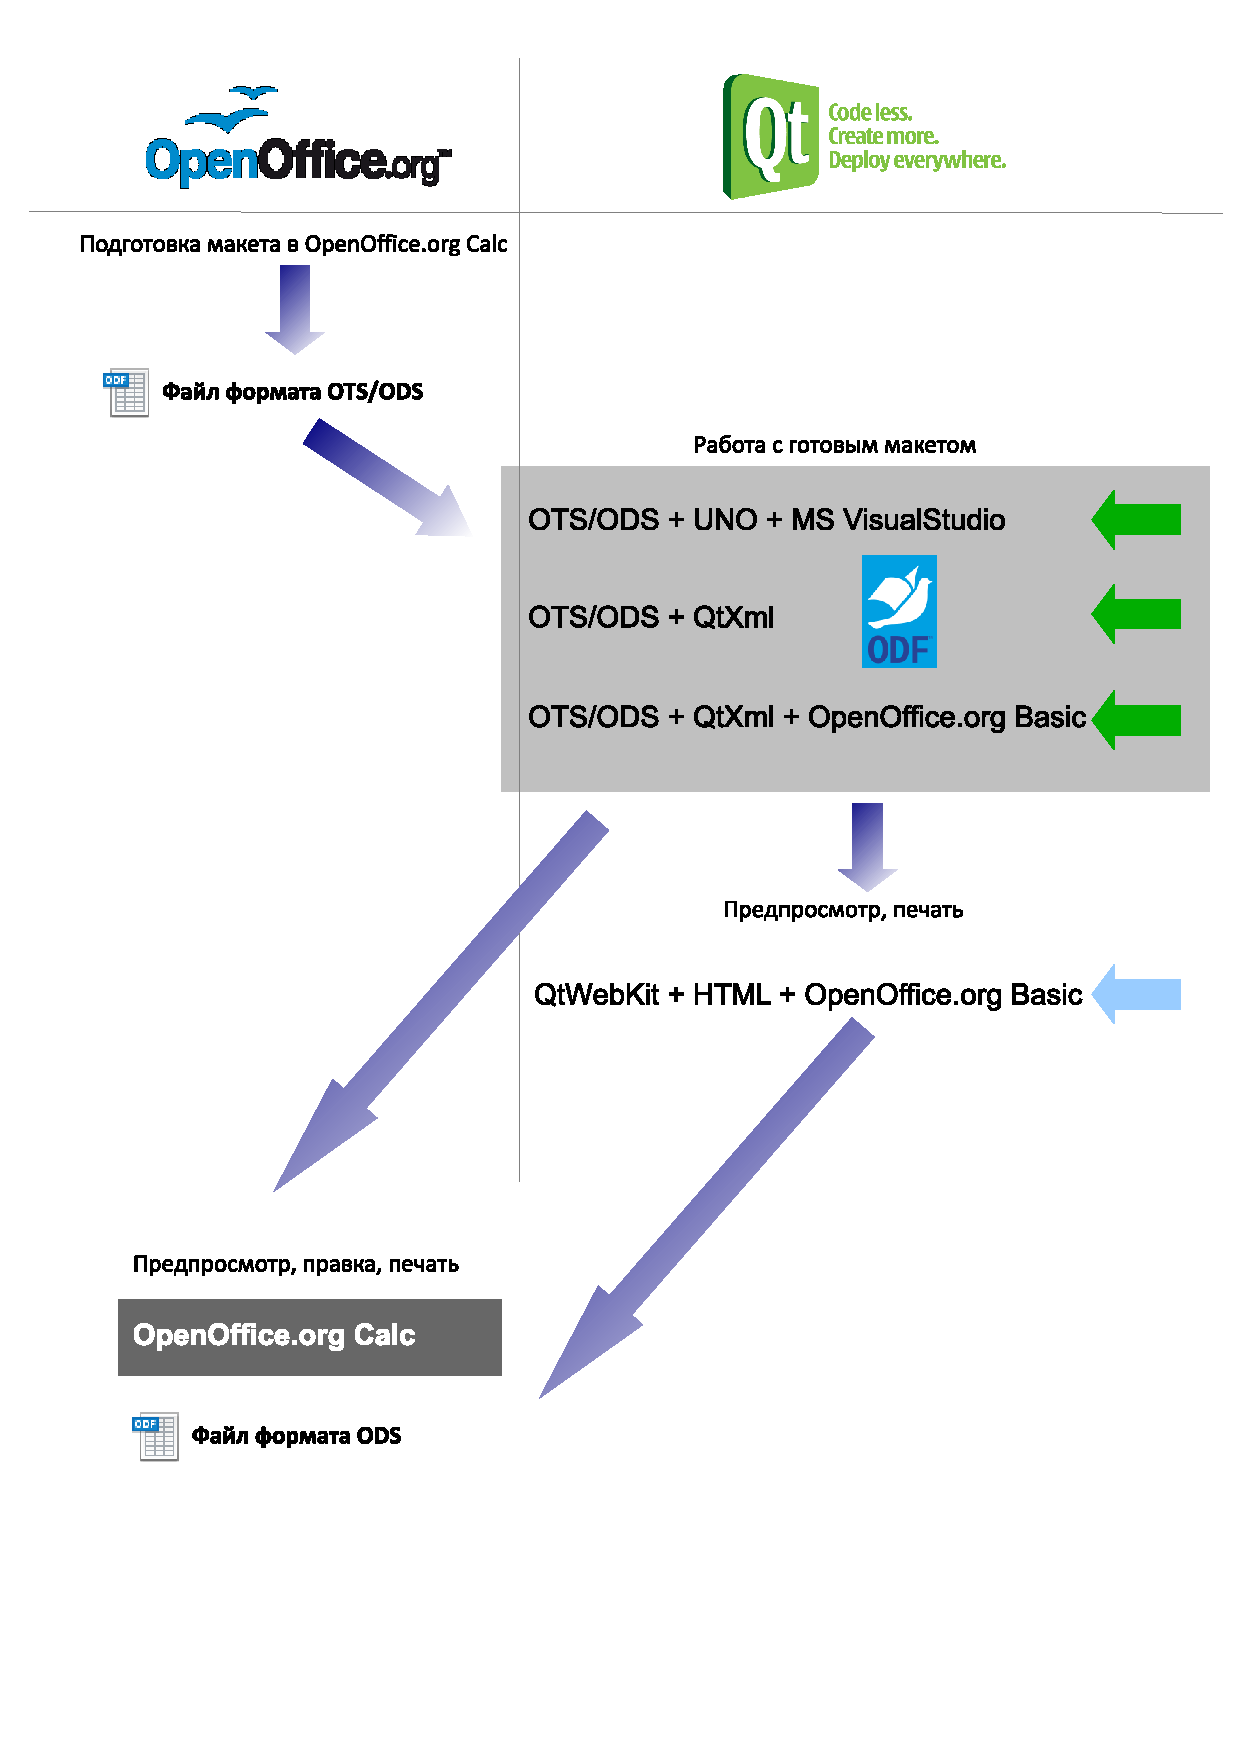
\includegraphics[height=0.6\textheight]{08_garanin}}
\end{figure}

\end{document}

%\documentclass[10pt, a5paper]{article}
\usepackage{pdfpages}
\usepackage{parallel}
\usepackage[T2A]{fontenc}
\usepackage{ucs}
\usepackage[utf8x]{inputenc}
\usepackage[polish,english,russian]{babel}
\usepackage{hyperref}
\usepackage{rotating}
\usepackage[inner=2cm,top=1.8cm,outer=2cm,bottom=2.3cm,nohead]{geometry}
\usepackage{listings}
\usepackage{graphicx}
\usepackage{wrapfig}
\usepackage{longtable}
\usepackage{indentfirst}
\usepackage{array}
\newcolumntype{P}[1]{>{\raggedright\arraybackslash}p{#1}}
\frenchspacing
\usepackage{fixltx2e} %text sub- and superscripts
\usepackage{icomma} % коскі ў матэматычным рэжыме
\PreloadUnicodePage{4}

\newcommand{\longpage}{\enlargethispage{\baselineskip}}
\newcommand{\shortpage}{\enlargethispage{-\baselineskip}}

\def\switchlang#1{\expandafter\csname switchlang#1\endcsname}
\def\switchlangbe{
\let\saverefname=\refname%
\def\refname{Літаратура}%
\def\figurename{Іл.}%
}
\def\switchlangen{
\let\saverefname=\refname%
\def\refname{References}%
\def\figurename{Fig.}%
}
\def\switchlangru{
\let\saverefname=\refname%
\let\savefigurename=\figurename%
\def\refname{Литература}%
\def\figurename{Рис.}%
}

\hyphenation{admi-ni-stra-tive}
\hyphenation{ex-pe-ri-ence}
\hyphenation{fle-xi-bi-li-ty}
\hyphenation{Py-thon}
\hyphenation{ma-the-ma-ti-cal}
\hyphenation{re-ported}
\hyphenation{imp-le-menta-tions}
\hyphenation{pro-vides}
\hyphenation{en-gi-neering}
\hyphenation{com-pa-ti-bi-li-ty}
\hyphenation{im-pos-sible}
\hyphenation{desk-top}
\hyphenation{elec-tro-nic}
\hyphenation{com-pa-ny}
\hyphenation{de-ve-lop-ment}
\hyphenation{de-ve-loping}
\hyphenation{de-ve-lop}
\hyphenation{da-ta-ba-se}
\hyphenation{plat-forms}
\hyphenation{or-ga-ni-za-tion}
\hyphenation{pro-gramming}
\hyphenation{in-stru-ments}
\hyphenation{Li-nux}
\hyphenation{sour-ce}
\hyphenation{en-vi-ron-ment}
\hyphenation{Te-le-pathy}
\hyphenation{Li-nux-ov-ka}
\hyphenation{Open-BSD}
\hyphenation{Free-BSD}
\hyphenation{men-ti-on-ed}
\hyphenation{app-li-ca-tion}

\def\progref!#1!{\texttt{#1}}
\renewcommand{\arraystretch}{2} %Іначай формулы ў матрыцы зліпаюцца з лініямі
\usepackage{array}

\def\interview #1 (#2), #3, #4, #5\par{

\section[#1, #3, #4]{#1 -- #3, #4}
\def\qname{LVEE}
\def\aname{#1}
\def\q ##1\par{{\noindent \bf \qname: ##1 }\par}
\def\a{{\noindent \bf \aname: } \def\qname{L}\def\aname{#2}}
}

\def\interview* #1 (#2), #3, #4, #5\par{

\section*{#1\\{\small\rm #3, #4. #5}}

\def\qname{LVEE}
\def\aname{#1}
\def\q ##1\par{{\noindent \bf \qname: ##1 }\par}
\def\a{{\noindent \bf \aname: } \def\qname{L}\def\aname{#2}}
}


\begin{document}

\title{Базовая серверная архитектура для высоконагруженного стартапа}

\author{Михаил Пянко\\
\small Минск, ООО Анакреон,\texttt{mihail.pianko@warecorp.com}
}
\maketitle

\begin{abstract}
This article describes how to create a good environment for start-up project: what kind of server do we need for each role, and how these servers should communicate. Architecture restrictions are considered. Technical and architecture suggestions are made.
\end{abstract}

На начальном этапе разработки стартапа многие разработчики сталкиваются с проблемой создания достаточно гибкой и в будущем масштабируемой архитектуры приложения, оптимизированной для большой нагрузки. Мы хотели бы поделиться опытом в этой области. В качестве примера рассмотрим методы построения ресурса, базирующегося на Ruby On Rails. Тем не менее примеры, которые будут приведены ниже, с легкостью могут быть использованы для LAMP-решений. 

\section*{Серверы можно разделить на несколько типов по ролям:}
\begin{itemize}
\item Application
\item Database 
\item Load Balancer
\item Utils
\item Tools
\end{itemize}

{\bf Application} --- это frontend-сервер. Возможно использование как одного, так и нескольких Application-серверов. В случае использования одного Application-сервера надобности в балансировке нагрузки нет.

Application сервер выполняет следующие функции:
\begin{itemize}
\item обработка запросов от пользователей (получает запросы от балансировщика нагрузки),
\item взаимодействие с базой данных (Database server),
\item отправка сообщений в очередь сообщений (Utils server),
\item взаимодействие с CDN,
\item взаимодействие с search engines (Util server),
\item инвалидация кэша,
\item работа с кэшем (Database server).
\end{itemize}

Application сервер не должен производить следующих действий:
\begin{itemize}
\item преобразование медиа контента (видео, аудио, слайдшоу, и т.д.),
\item преобразование/кропинг картинок (если позволяет архитектура),
\item отправка сообщений электронной почты (если позволяет архитектура),
\item запросы на сторонние ресурсы через RestClient, curl, etc. (если позволяет архитектура).
\end{itemize}
{\bf Database} --- сервер, на котором находится база данных. В некоторых случаях на Database-сервер также устанавливается memcached, но это зависит от загрузки и конфигурации Database-сервера. 

Database-сервер выполняет следующие функции:
\begin{itemize}
\item обработка запросов от Application и Utils серверов,
\item хранение кэша (в случае установки memcached на DB сервер).
\end{itemize}
{\bf Load Balancer} --- балансировщик нагрузки, необходимый для распределения запросов пользователей между Application-серверами. Простейшим решением является использование nginx в качестве балансировщика нагрузки.

Load Balancer выполняет следующие функции:
\begin{itemize}
\item распределение запросов между Application серверами,
\item обработка HTTPS соединений (SSL сертификат должен быть сконфигурирован на балансировщике),
\item кэширование при использовании Varnish или связки nginx + memcache,
\item Firewall.
\end{itemize}

{\bf Utils} --- сервер, на котором располагаются сопутствующие сервисы, необходимые для отложенной обработки данных. Вот краткий список:
\begin{itemize}
\item message queue (RabbitMQ, Apache Message Queue, etc),
\item search engines (Solr, Sphinx, etc),
\item обработчики сообщений,
\item сервисы для обработки Video, Audio, SlideShow,
\item отправка сообщений электронной почты,
\item взаимодействие с CDN,
\item инвалидация кэша,
\item взаимодействие со сторонними ресурсами (PDF converters, \linebreak SendGrid, etc.). 
\end{itemize}
{\bf Tools} "--- сервер, необходимый для установки сторонних решений для работы приложения. В частности, приложения, базирующиеся на Java/Tomcat, система мониторинга и ресурсы, в безопасности которых вы сомневаетесь (Spellchecker, etc.). Tools-сервер не может установить соединения с Application, Database, Utils-серверами. Единственный протокол взаимодействия "--- это HTTP. Это дает гарантию того, что в результате взлома стороннего компонента основная ферма не пострадает. Сервер с этой ролью не обязателен. 


\begin{figure}[ht]
\centering{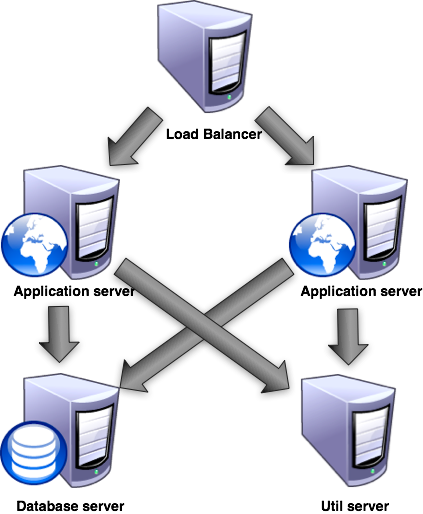
\includegraphics[width=8cm]{09_pianko.png}}
\label{pic:fl1}
%\caption{~}
\end{figure}

\section*{Ограничения, которые накладываются на архитектуру приложения}

\subsection*{Хранение кэша}
Необходимо организовать централизованное хранилище кэша. Файловый кэш и кэширование данных в памяти сервера работать не будет, так как кэш может создаваться и инвалидироваться с разных серверов. Наилучшим решением в данном случае является использования memcached. 

\subsection*{Хранение сессий пользователя}
В данном случае целесообразно хранить сессии в memcached или в Cookies. Отдача сессии на сторону пользователя --- менее безопасное и более медленное решение, чем хранение в memcached. 

\subsection*{Хранение медиа-данных пользователя}
Любой контент, загруженный пользователем на сервер, не может быть просто  сохранен в папку /public/upload. Наилучшим способом хранения данных является CDN. 

\subsection*{Рекомендации по автоматизированной конфигурации серверов}
Существует достаточно большое количество ПО для поддержания конфигурации серверов: Сfengine, Puppet, Chef, Sprinkle. 

Для автоматизированного конфигурирования серверов мы используем Sprinkle. Sprinkle --- это достаточно простое приложение на RoR, позволяющее разрабатывать сценарии по установке ПО на UNIX"=сервера.  Sprinkle поддерживает разделение серверов на роли, фермы и т.д. Так же поддерживаются различные типы инсталяторов, методов проверки текущей конфигурации, источников данных. Sprinkle имеет открытый исходный код, что позволяет вносить изменения в логику работы отдельных компонентов или создавать дополнительные модули. 

\section*{Варианты инсталляции}
Существует несколько вариантов ферм.
\begin{itemize}
\item Single server installation.
  \begin{itemize}
  \item На одном сервере располагаются Application + Util + Database
  \end{itemize}
\item Light farm
  \begin{itemize}
  \item $1$ сервер: Application 
  \item $1$ сервер: Util + DB
  \end{itemize}
\item Big farm:
  \begin{itemize}
  \item $1$ сервер: Load Ballancer 
  \item $x$ серверов: Application
  \item $1-x$ серверов: Util 
  \item $1-x$ серверов: Database (о репликациях и масштабировании базы данных можем поговорить чуть позже) 
  \end{itemize}
\end{itemize}
На самом деле существует множество комбинаций распределения ролей по физическим серверам. Необходимо выбирать оптимальный вариант в зависимости от нагрузки на сервера каждой роли. 

\section*{Рекомендации по архитектуре. Несколько примеров}

\subsection*{Интеграция со сторонними ресурсами}
Зачастую необходима интеграция со сторонними ресурсами для преобразования видео и аудио, обработки слайд-шоу, отсылки писем и т.д. 

Это подразумевает установку соединения по протоколам TCP, HTTP, etc. 
В данном случае существует несколько рисков:
\begin{itemize}
\item сервер недоступен
\item сервер перегружен 
\end{itemize}

В первом случае пользователь не сможет завершить действие, часть данных может быть потеряна или пользователь увидит сообщение ошибки на экране. 
Во втором случае мы получим очень долгую обработку страницы, что доставит неудобство пользователю. 

Лучшим решением в данном случае является отправка события в очередь сообщений и обработка на стороне util"=сервера. 

\subsection*{Обработка картинок пользователя}
Если ваш ресурс поддерживает возможность загрузки аватаров пользователей, логотипов с последующим ресайзингом изображений, вы можете столкнуться с проблемой большой нагрузки на сервер. 

Есть несколько распространенных методов ресайзинга изображений:

\begin{itemize}
\item оригинальное изображение сохраняется в хранилище без обработки. Доступ к изображению со страниц сайта реализован через врапер с элементарной логикой. Если картинка сгенерирована, то необходимо отдать ее через STDOUT или вернуть редирект на статический. Если картинка отсутствует, то сгенерировать и выполнить предыдущий шаг. Проблема этого метода в том, что нагрузка, которую может создать данный алгоритм, не может быть спрогнозирована.  При добавлении нового размера изображения достаточно визита поискового бота - и скорее всего сервера будут перегружены. 
\item оригинальное изображение преобразуется в нужные форматы и размеры непосредственно после загрузки на сервер. Это дает единовременную нагрузку на Application-сервера. Минусом данного метода является задержка в возврате страницы пользователю, что может вызвать дискомфорт.
\item последний вариант является модифицированной версией \linebreak предыдущего. Вместо непосредственной обработки изображения на Application-сервере необходимо отправить событие в очередь сообщения и произвести обработку изображения на Util"=сервере. 
\end{itemize}

\section*{Заключение}

Выше приведены приемы для построения начальной архитектуры высоконагруженной системы, которая в будущем может быть легко расширена и  смасштабирована. Способы дальнейшего развития напрямую зависят от архитектуры приложения, нагрузки на отдельные узлы системы и специфики проекта.

\end{document}





%\documentclass[10pt, a5paper]{article}
\usepackage{pdfpages}
\usepackage{parallel}
\usepackage[T2A]{fontenc}
\usepackage{ucs}
\usepackage[utf8x]{inputenc}
\usepackage[polish,english,russian]{babel}
\usepackage{hyperref}
\usepackage{rotating}
\usepackage[inner=2cm,top=1.8cm,outer=2cm,bottom=2.3cm,nohead]{geometry}
\usepackage{listings}
\usepackage{graphicx}
\usepackage{wrapfig}
\usepackage{longtable}
\usepackage{indentfirst}
\usepackage{array}
\newcolumntype{P}[1]{>{\raggedright\arraybackslash}p{#1}}
\frenchspacing
\usepackage{fixltx2e} %text sub- and superscripts
\usepackage{icomma} % коскі ў матэматычным рэжыме
\PreloadUnicodePage{4}

\newcommand{\longpage}{\enlargethispage{\baselineskip}}
\newcommand{\shortpage}{\enlargethispage{-\baselineskip}}

\def\switchlang#1{\expandafter\csname switchlang#1\endcsname}
\def\switchlangbe{
\let\saverefname=\refname%
\def\refname{Літаратура}%
\def\figurename{Іл.}%
}
\def\switchlangen{
\let\saverefname=\refname%
\def\refname{References}%
\def\figurename{Fig.}%
}
\def\switchlangru{
\let\saverefname=\refname%
\let\savefigurename=\figurename%
\def\refname{Литература}%
\def\figurename{Рис.}%
}

\hyphenation{admi-ni-stra-tive}
\hyphenation{ex-pe-ri-ence}
\hyphenation{fle-xi-bi-li-ty}
\hyphenation{Py-thon}
\hyphenation{ma-the-ma-ti-cal}
\hyphenation{re-ported}
\hyphenation{imp-le-menta-tions}
\hyphenation{pro-vides}
\hyphenation{en-gi-neering}
\hyphenation{com-pa-ti-bi-li-ty}
\hyphenation{im-pos-sible}
\hyphenation{desk-top}
\hyphenation{elec-tro-nic}
\hyphenation{com-pa-ny}
\hyphenation{de-ve-lop-ment}
\hyphenation{de-ve-loping}
\hyphenation{de-ve-lop}
\hyphenation{da-ta-ba-se}
\hyphenation{plat-forms}
\hyphenation{or-ga-ni-za-tion}
\hyphenation{pro-gramming}
\hyphenation{in-stru-ments}
\hyphenation{Li-nux}
\hyphenation{sour-ce}
\hyphenation{en-vi-ron-ment}
\hyphenation{Te-le-pathy}
\hyphenation{Li-nux-ov-ka}
\hyphenation{Open-BSD}
\hyphenation{Free-BSD}
\hyphenation{men-ti-on-ed}
\hyphenation{app-li-ca-tion}

\def\progref!#1!{\texttt{#1}}
\renewcommand{\arraystretch}{2} %Іначай формулы ў матрыцы зліпаюцца з лініямі
\usepackage{array}

\def\interview #1 (#2), #3, #4, #5\par{

\section[#1, #3, #4]{#1 -- #3, #4}
\def\qname{LVEE}
\def\aname{#1}
\def\q ##1\par{{\noindent \bf \qname: ##1 }\par}
\def\a{{\noindent \bf \aname: } \def\qname{L}\def\aname{#2}}
}

\def\interview* #1 (#2), #3, #4, #5\par{

\section*{#1\\{\small\rm #3, #4. #5}}

\def\qname{LVEE}
\def\aname{#1}
\def\q ##1\par{{\noindent \bf \qname: ##1 }\par}
\def\a{{\noindent \bf \aname: } \def\qname{L}\def\aname{#2}}
}


\begin{document}
\title{Мониторинг Linux/FreeBSD серверов}
\author{Николай Маржан\footnote{Киев, Украина, PortaOne, Inc. \url{delgod@delgod.com}}}

\maketitle



\begin{abstract}Purposes and functions of monitoring systems are discussed, as far as general approaches to analyze the diagnostic parameters of a server. Observed information is classified into parameters received from hardware maintenance, operating system, services and typical database. Sample diagnostic parameters are presented for each category.
\end{abstract}

К стандартным целям проводимого на серверах мониторинга можно отнести:
\begin{itemize}
	\item Отслеживание критических значений диагностических параметров состояния и уведомление инженеров об их появлении.
	\item Накопление статистической информации для последующего анализа.
\end{itemize}

Уведомление о том, что система находится в критическом состоянии, является наиболее важной функцией мониторинга, так как требует немедленного вмешательства инженеров, которые занимаются поддержкой данной системы.

Даже если проблема носит временный характер (например, стопроцентная загрузка процессора, возникшая спонтанно и затем прекратившаяся через 20 минут), выяснить причину такого поведения можно только тогда, когда проблема присутствует (причиной могла быть удаленная DOS-атака).

Накопление статистической информации происходит обычно в 2-х видах:
\begin{itemize}
	\item Лог-файлы. Обычно в них записываются только те моменты, когда система входит в критическое состояние, и когда возващается в нормальное.
	\item Данные для графиков по каждому показателю.
\end{itemize}

Графики --- не менее важная часть системы мониторинга, так как только они позволяют проводить анализ состояния сервера в целом, как сложной системы. 
Используя графики для наблюдения динамики диагностических параметров, мы можем:
\begin{itemize}
	\item Увидеть, в каком состоянии находился сервер в любой момент времени в прошлом. Мы можем быстро понять, чем отличается сегодняшнее состояние от состояния недельной давности.
	\item Проследить закономерности возможной взаимосвязи между диагностическими параметрами. Например, когда повышается входящий трафик на сетевом интерфейсе --- повышается нагрузка на центральный процессор.
	\item Находить противоречия между значениями диагностических параметров. Например, сильно возросло количество запросов на чтение к базе данных, и база данных начала использовать на 1 Гб больше оперативной памяти, но при этом с жесткого диска было считано всего 100 Мб данных.
 Увидеть, в каком состоянии находился сервер в любой момент времени в прошлом. Мы можем быстро понять, чем отличается сегодняшнее состояние от состояния недельной давности.
	\item Проследить закономерности возможной взаимосвязи между диагностическими параметрами. Например, когда повышается входящий трафик на сетевом интерфейсе --- повышается нагрузка на центральный процессор.
	\item Находить противоречия между значениями диагностических параметров. Например, сильно возросло количество запросов на чтение к базе данных, и база данных начала использовать на 1 Гб больше оперативной памяти, но при этом с жесткого диска было считано всего 100 Мб данных.
\end{itemize}
Диагностическими параметрами состояния для аппаратного обеспечения являются: 
\begin{enumerate}
	\item температура центрального процессора;
	\item наличие повреждённых секторов или ошибок чтения на жестком диске;
	\item состояние аппаратного RAID-контроллера.
\end{enumerate}
К диагностическим параметрам состояния для операционной системы можно отнести:
\begin{enumerate}
	\item количество задач, ожидающих выполнения (load average);
	\item время простоя центрального процессора (idle);
	\item время простоя каждого ядра центрального процессора (idle);
	\item размер свободного места на жестком диске;
	\item нагрузка на жесткий диск;
	\item количество данных в разделе подкачки (swap);
	\item активная запись или чтение с раздела подкачки (swaping/paging);
	\item количество использованной памяти;
	\item количество памяти, потребляемой каждым приложением;
	\item скорость передачи данных на сетевых интерфейсах;
	\item подтверждение того, что сетевые интерфейсы работают на нужной скорости и в полнодуплексном режиме;
	\item количество ошибок и коллизий на сетевых интерфейсах;
	\item состояние системных буферов (freebsd vm.zone), mbuf clusters, sendfile-буферов, размер KVM, Pipe KVA;
	\item количество открытых файлов, количество открытых сокетов;
	\item отсутствие процессов-зомби;
	\item отсутствие ошибок сегментации у процессов.
\end{enumerate}
Диагностическими параметрами состояния сервисов являются:
\begin{enumerate}
	\item подтверждение того, что все критически важные сервисы запущены.
	\item подтверждение того, что сервисы успевают вычитывать данные из входящей очереди сетевой подсистемы.
	\item подтверждение того, что нет отброшенных данных вследствие полных буферов соединения (dropped due to full socket buffers).
\end{enumerate}
Диагностическими параметрами состояния базы данных MySQL являются:
\begin{enumerate}
	\item количество максимально использованных соединений;
	\item количество запросов, количество медленных запросов;
	\item количество операций записи/чтения с жесткого диска;
	\item отставание репликации.
\end{enumerate}
Как показал опыт построения систем мониторинга в гетерогенных сетях, подходы и диагностические параметры практически идентичны для операционных систем FreeBSD и Linux; основные различия связаны с мониторингом системных буферов и с некоторыми расхождениями в синтаксисе команд.
\end{document}

%\documentclass[10pt, a5paper]{article}
\usepackage{ucs}
\usepackage[utf8]{inputenc}
\usepackage[T2A]{fontenc}
\usepackage[english, russian]{babel}
\usepackage{hyperref}
\usepackage{geometry}
\frenchspacing
\begin{document}
\title{Darktable, приложение для каталогизации и обработки RAW-файлов}
\author{Константин Шевцов\footnote{Новополоцк/Минск, Беларусь, \url{kanstantsin.sha@gmail.com}}, Александр Рабцевич\footnote{Минск, Беларусь, \url{alexander.v.rabtchevich@gmx.net}}}
\date{}

\def\progref!#1!{\texttt{#1}}

\maketitle

\begin{abstract}
Darktable is an open source application devoted to processing of RAW files. The program can manage collections of RAWs with rating, color labels and custom tags. A rich set of build-in filters (some of them are unique), used at processing, store their settings in a form of a history stack, which is saved alongside original RAW, providing original RAW untouched. Due to rawspeed RAW importing library, multi-threading and permanent optimizations, the program is fast and responsive.
\end{abstract}

\section*{История}
В докладе описывается история появления и развития проекта, возможности программы на примере работы с RAW файлами, а также планы разработчиков по развитию программы.

До появления darktable в ОС Linux отсутствовал открытый инструмент, сочетающий возможности каталогизации коллекции RAW файлов с их неразрушающей обработкой. UFRaw и  Rawtherapee не обладают достаточными возможностями для профессионального фотографа.

Восполнить пробел решил Йоханес Ханика (Johannes Hanika), который зарегистрировал проект darktable на SourceForge в феврале 2009 года. Вскоре к нему присоединились 3 разработчика: Хенрик Андерсон (Henrik Andersson), Паскаль де Брайн (Pascal de Bruijn), Александр Прокудин. В настоящее время у проекта около 20 контрибьюторов. 

\section*{Описание}
Спиосок основных возможностей программы при работе с коллекцией включает:
\begin{itemize}
\item импорт фотографий в коллекцию из папки, импорт отдельных фотографий. Фотографии физически не перемещаются.
\item импорт из фотоаппарата посредством gPhoto2
\item хранение данных о коллекции в собственной базе данных
присвоение фотографиям рейтинга (stars), система цветовых меток, пользовательские теги (метки).
\item поиск по произвольной комбинации: съемка, камера, метка, дата, наличие изменений после экспорта.
\item копирование истории обработки между фотографиями
\item экспорт в jpeg, tiff (8 и 16 бит) 
\item экспорт в picasa, flickr, email
Основные возможности программы по обработке RAW (версия из репозитария git):
\item внутреннее представление данных RGB float (32 бит/канал) или LCh (в зависимости от модуля)
\item быстрый предосмотр с масштабированием вплоть до 100\%, при предосмотре обрабатывается только часть изображения, показываемая в окне с кешированием операций
\item многопоточность
\item использование для ряда операций OpenCL при наличии драйвера и подходящего графического ускорителя
\item все изменения хранятся в виде стека истории с возможностью отката до произвольной точки, а также копирования истории изменений между фотографиями или сохранения ее в виде стиля для последующего применения
\item стек истории сохраняется в виде *.xmp файла вместе с оригинальным файлом RAW
\item модульная архитектура (плагины)
\item возможность создания и ручного/автоматического использования предустановок для всех модулей
\item наличие режимов смешивания для большинства модулей
\item алгоритмы дебайеризации ppg и AMaZE 
\item поканальный баланс белого через множители либо через  - сдвиг цветовой температуры и множителя зеленого канала
\item редактируемая тональная кривая камеры с возможностью выбора из набора готовых кривых, аналогичных используемым производителями цифровых фотоаппаратов
\item восстановление пересветов при отрицательной экспокоррекции
\item профили камеры: стандартные (Adobe), улучшенные, либо пользовательские
\item трансформации: кадрирование с выбираемым соотношением сторон, поворот, перспектива
\item редактируемая тональная кривая (L канал в LCh пространстве
\item возможность работать с тональной кривой в виде последовательности зон Адамса
\item мощнейший инструмент --- эквалайзер, позволяющий регулировать локальный контраст (L и С) в зависимости от пространственной частоты (аналога радиуса в USM) с помощью избегающих краев вейвлетов
\item подавление шума
\item исправление геометрических искажений оптики с помощью библиотеки lensfun
\item регулирование яркости/насыщенности или сдвига тонов в плагине цветовые зоны
\item микшер каналов
\item обесцвечивание с регулируемым цветовым фильтром
\item градиентный фильтр (GND) с возможностью поворота и радиального смещения
\item эффект виньетирования с регулируемыми на холсте радиусом, формой (окружность/эллипс)
\item вельвия
\item смягчающий фильтр
\item и другие фильтры
\end{itemize}

\section*{Будущее}
В настоящее время разработчики готовят программу к выпуску версии 0.9. 

В ближайших планах разработчиков --- добавление функционала масок (Henrik Andersson) и переработка интерфейса с централизованной обработкой горячих клавиш (GSoC студент Robert Bieber). В состоянии обсуждения — возможность не  однократного использования плагинов. В более отдаленных планах — использование GEGL внутри darktable с возможностью передачи данных в GIMP и обратно для более сложного редактирования; однако этот функционал может появиться не раньше выхода GIMP 3.0.

Проект активно развивается и радует постоянное растущее сообщество пользователей новыми выпусками с периодичностью примерно раз в три месяца. Можно ответственно заявить, что текущая версия пригодна для использования профессиональным фотографом.

\begin{thebibliography}{9}
\bibitem{pDynamo} Официальный сайт проекта --- \url{http://darktable.sf.net}
\end{thebibliography}
\end{document}

%\documentclass[10pt, a5paper]{article}
\usepackage{ucs}
\usepackage[utf8]{inputenc}
\usepackage[T2A]{fontenc}
\usepackage[english, russian]{babel}
\usepackage{hyperref}
\usepackage{geometry}
\frenchspacing

\begin{document}

\title{On Digital Monies}

\author{Daniel Nagy\footnote{Budapest, Hungary, ePoint Systems Ltd., \url{nagydani@epointsystem.org}}}
\date{}
\maketitle
\renewcommand{\abstractname}{Abstract}
\begin{abstract}
Payment over digital communications networks has been a hot topic since
the introduction of the telegraph, the first such electronic network;
originally, Western Union was a telegraph company. Money, however, is
more than a means of payment: it is also an instrument of saving and
credit, a measure of value and a unit of accounting. In my presentation,
I shall explore various attempts at creating digital money, both
proprietary and open-source, theoretical and practical.
\end{abstract}

The main difference between digitally represented information and
everything else that has been historically used as money is that unlike
the latter, digital information can be copied at no cost, with perfect
fidelity in essentially unlimited quantities. Very undesirable
properties for something that we intend to use as money. This is the
main technical challenge in using digital information as money (known as
``double spending''). How can we make sure that no more gets spent than
what has been earned?

There is, however, a different, no less interesting challenge that is
not purely technical: how to get actual people provide real value in
exchange for pieces of digital information. Why would people use pieces
of digital information as a means of exchange or to keep their savings
or to measure value?

The third challenge is a legal one. Since the first ever gold coins have
been minted at the behest of Croesus, King of Lydia in the sixth
century, B.C., money has been subject of government regulation and very
often exclusive monopoly. How can digital money exist within the current
legal framework?

Different solutions to these challenges have been proposed. We shall
explore the solutions to these challenges in the following systems in
some technical detail:

\subsubsection*{DigiCash}
David Chaum's company founded in 1990 on the basis of some clever
cryptography -- blind digital signatures -- he published in 1988. The
company declared bankruptcy in 1998, but in many ways it provided
inspiration to the many ventures that followed. I brief and simplified
introduction to the technology will be given as well as what I think
were the reasons for failure.

\subsubsection*{WebMoney}
Artiom Genkin went the other route: his doctoral thesis on the topic
followed business success. Founded in 1998, WebMoney made its name by
proving to be more resilient in the face of financial meltdown than the
Russian banking sector. To this day, WebMoney is one of the most
sophisticated and successful digital money, albeit mostly in the
Russian-speaking world.

\subsubsection*{BitCoin}
This is an open-source project started in 2009 by the mysterious Satoshi
Nakatomo, based on earlier research either done or popularized by Nick
Szabo (a former DigiCash employee). This year, BitCoin's popularity (and
valuation) exploded, making it one of the most important and interesting
innovations in the field.

\subsubsection*{ePoint}
This is my own open-source project, kicked off in 2005. However, I am
not going to talk much about how it works now; rather, I shall outline
where I would like to take it and what needs to be done to get there.
Maybe, I like-minded developers of open-source software among LVEE 2011
participants will join me in creating something valuable and useful.


\end{document}





%\documentclass[10pt, a5paper]{article}
\usepackage{ucs}
\usepackage[utf8]{inputenc}
\usepackage[T2A]{fontenc}
\usepackage[english, russian]{babel}
\usepackage{hyperref}
\usepackage{geometry}
\usepackage{graphicx}
\frenchspacing

\begin{document}

\title{Linux и СПО в создании музыки и живом исполнении. Обзор имеющихся программ и ниши применения}
\author{Сергей Васильев\footnote{Таллинн, Эстония, \url{zyxos2@gmail.com}}}
\date{}
\maketitle
\begin{abstract}
The aspects of using Linuz and free software in amateur music creation, sound editing and live performances are reviewed.
\end{abstract}

Ещё несколько лет назад Linux был малопригоден для работы со звуком; за последние годы ситуация значительно изменилась: улучшилась поддержка многих звуковых карт, MIDI-контроллеров и MIDI-интерфейсов, появились новые программы, интерфейс которых изменился в лучшую сторону, что снизило порог вхождения для начинающих пользоваталей. И, несмотря на некоторые всё ещё присутствующие проблемы, сейчас вполне возможно использование решений на базе Linux и СПО в любительской музыкальной деятельности. Применение данных решений имеет ряд преимуществ, одним из которых является низкая стоимость, что немаловажно для начинающих музыкантов. 

Многие начинающие музыканты не обращают внимания на Linux из-за недостаточной информированности, и очень часто для выполнения простых задач прибегают к применению программного обеспечения, возможности которого на порядок превышают потребности, что приводит к нерациональному расходу денежных средств или к незаконному использованию коммерческих приложений. Имеющейся на данный момент программной базы и поддержки оборудования достаточно для выполнения основных задач. 

В таблице приведены категории и некоторые программы, которые, после сравнительного анализа, были отобраны как наиболее подходящие для использования в сетапе для демонстрации.

\begin{figure}[ht]
\centering{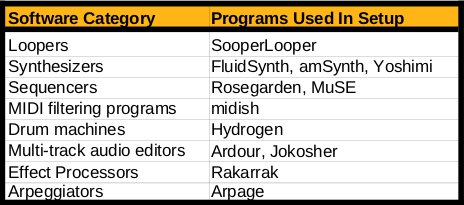
\includegraphics[width=8cm]{13_abstract.jpg}}
%\label{pic:fl1}
\caption{Приложения по категориям}
\end{figure}

По субъективной оценке, наиболее заполнены категории многодорожечных аудиоредакторов, представленных мощнейшим проектом Ardour, и некоторыми более простыми; процессоров эффектов --- Rakarrak и др.; также почти на 100\% покрывает потребности замечательный редактор табулатур TuxGuitar.

Драм-машины представлены практически одним проектом Hydrogen, но довольно мощным, лишь с небольшими пожеланиями усовершенствований в области мульти-лэйеринга.

Что касается луперов и арпеджиаторов --- лидеры SooperLooper и Arpage предоставляют базовую функциональность, но хотелось бы надеяться на улучшения в будущем.

Категории с некоторым количеством недочетов --- секвенсеры и MIDI-фильтры.

Проблемные категории --- синтезаторы (несмотря на замечательные программы FluidSynth, amSynth и Yoshimi, ситуация  c VST-плагинами все еще далека от идеальной) и автоаккомпаниаторы (поскольку MMA очень сильно нехватает адекватного GUI).
\end{document}

%\documentclass[10pt, a5paper]{article}
\usepackage{pdfpages}
\usepackage{parallel}
\usepackage[T2A]{fontenc}
\usepackage{ucs}
\usepackage[utf8x]{inputenc}
\usepackage[polish,english,russian]{babel}
\usepackage{hyperref}
\usepackage{rotating}
\usepackage[inner=2cm,top=1.8cm,outer=2cm,bottom=2.3cm,nohead]{geometry}
\usepackage{listings}
\usepackage{graphicx}
\usepackage{wrapfig}
\usepackage{longtable}
\usepackage{indentfirst}
\usepackage{array}
\newcolumntype{P}[1]{>{\raggedright\arraybackslash}p{#1}}
\frenchspacing
\usepackage{fixltx2e} %text sub- and superscripts
\usepackage{icomma} % коскі ў матэматычным рэжыме
\PreloadUnicodePage{4}

\newcommand{\longpage}{\enlargethispage{\baselineskip}}
\newcommand{\shortpage}{\enlargethispage{-\baselineskip}}

\def\switchlang#1{\expandafter\csname switchlang#1\endcsname}
\def\switchlangbe{
\let\saverefname=\refname%
\def\refname{Літаратура}%
\def\figurename{Іл.}%
}
\def\switchlangen{
\let\saverefname=\refname%
\def\refname{References}%
\def\figurename{Fig.}%
}
\def\switchlangru{
\let\saverefname=\refname%
\let\savefigurename=\figurename%
\def\refname{Литература}%
\def\figurename{Рис.}%
}

\hyphenation{admi-ni-stra-tive}
\hyphenation{ex-pe-ri-ence}
\hyphenation{fle-xi-bi-li-ty}
\hyphenation{Py-thon}
\hyphenation{ma-the-ma-ti-cal}
\hyphenation{re-ported}
\hyphenation{imp-le-menta-tions}
\hyphenation{pro-vides}
\hyphenation{en-gi-neering}
\hyphenation{com-pa-ti-bi-li-ty}
\hyphenation{im-pos-sible}
\hyphenation{desk-top}
\hyphenation{elec-tro-nic}
\hyphenation{com-pa-ny}
\hyphenation{de-ve-lop-ment}
\hyphenation{de-ve-loping}
\hyphenation{de-ve-lop}
\hyphenation{da-ta-ba-se}
\hyphenation{plat-forms}
\hyphenation{or-ga-ni-za-tion}
\hyphenation{pro-gramming}
\hyphenation{in-stru-ments}
\hyphenation{Li-nux}
\hyphenation{sour-ce}
\hyphenation{en-vi-ron-ment}
\hyphenation{Te-le-pathy}
\hyphenation{Li-nux-ov-ka}
\hyphenation{Open-BSD}
\hyphenation{Free-BSD}
\hyphenation{men-ti-on-ed}
\hyphenation{app-li-ca-tion}

\def\progref!#1!{\texttt{#1}}
\renewcommand{\arraystretch}{2} %Іначай формулы ў матрыцы зліпаюцца з лініямі
\usepackage{array}

\def\interview #1 (#2), #3, #4, #5\par{

\section[#1, #3, #4]{#1 -- #3, #4}
\def\qname{LVEE}
\def\aname{#1}
\def\q ##1\par{{\noindent \bf \qname: ##1 }\par}
\def\a{{\noindent \bf \aname: } \def\qname{L}\def\aname{#2}}
}

\def\interview* #1 (#2), #3, #4, #5\par{

\section*{#1\\{\small\rm #3, #4. #5}}

\def\qname{LVEE}
\def\aname{#1}
\def\q ##1\par{{\noindent \bf \qname: ##1 }\par}
\def\a{{\noindent \bf \aname: } \def\qname{L}\def\aname{#2}}
}


\begin{document}

\title{Amazon auto-scaling. Создание и оптимизация автомасштабируемых систем на базе GNU/Linux}
\author{Виктор Краев\footnote{Минск, Беларусь, \url{anakreon.by}}}
\date{}
\maketitle
\begin{abstract}\noindent 
The technology of auto-scaling clasters provided by Amazon for its cloud services is reviewed. Approach to monitor and control such cloud-based system is presented, as far as practical expe\-ri\-ence of migrating to the auto-scaled services.
\end{abstract}

\section*{Amazon EC2. Cloud vs Hardware}
С каждым годом IT-индустрия набирает обороты, но как бы не развивались технологии, ресурс выработки железа пока никто не победил. Отказ оборудования по-прежнему является одной из главных проблем современного хостинга. Конечно же, всегда есть возможность создания избыточности, но это тянет за собой достаточно серьезные расходы на дополнительное оборудование и его обслуживание. Поэтому наша компания обратила внимание на облачные вычисления. Наиболее продвинутой компанией, способной решить наши задачи, на сегодняшний день оказалась Amazon. Хотя их технология Elastic Cloud --- местами сырая, она находится в активной разработке и интегрируется с другими сервисами, нивелирующими ее недостатки. Не победив проблему «железа», в Amazon создали избыточность, покрыв недостатки другими сервисами, и сегодня падение инстансов (instances) или потеря данных в облаке иногда присутствует, но успешно компенсируется резервным копированием и высокой скоростью создания инстансов из резервных копий. Интеграция с такими сервисами, как auto-scaling, cloudwatch, cloudformation, позволяет добиться избыточности, намного превышающей возможности обычного кластера серверов, не задумываясь о «железе».  

\section*{Amazon Auto-Scaling. Hardware cluster vs scalable cloud}

На сегодняшний день для увеличения доступности и избыточности ресурса используют технологии кластеризации. Статический кластер подразумевает под собой использование определенного неизменяемого количества (больше 1) серверов, нагрузку между которыми распределяет балансировщик (Load Balancer). Это хорошее решение для ресурсов с постоянно высокой нагрузкой. Динамический кластер --- это кластер, где распределение нагрузки осуществляется между серверами, количество которых может меняться в зависимости от нужд и нагруженности проекта. Однако в «железе» это трудноосуществимо, т.к. тянет за собой целый шлейф проблем, связанных с установкой оборудования, разворачиванием ПО, а главное --- времени. С помощью сервиса EC2 на создание виртуального сервера уходит несколько минут. Создание происходит из уже готового образа (image), т.~е. выполняется клонирование существующей системы. Обычно это образы «чистых» систем, в которых установлены лишь базовые пакеты. Но Amazon позволяет создавать собственные образы уже настроенных и готовых к использованию систем --- например, хостинговых. Полученные образы помещаются в приватное хранилище, из которого в любой момент можно создать и отправить в работу клон. Эта технология, лежащая в основе создания динамического кластера и известная как AMI, позволяет мгновенно создавать кластеры различного размера. Для распределения нагрузки между элементами кластера используется сервис ELB (Elastic Load Balancer), который позволяет менять размерность кластера путем добавления или удаления виртуальных серверов в балансировщик. Однако, используя лишь web-интерфейс, вы сможете управлять кластером только вручную. Это значит, что если один из элементов кластера откажет в обслуживании, то балансировщик выбросит его из пула обрабатываемых запросов, и новый виртуальный сервер не встанет на его место автоматически. Чтобы автоматизировать этот процесс в Amazon придумали технологию Auto-Scaling. Эта технология позволяет задавать размерность кластера и использует проверку здоровья (health cheacking) серверов из ELB или EC2. В случае падения на место упавшего сервера из образа автоматически создается новый сервер и добавляет его в балансировщик. Сегодня управление конфигурацией Auto-Scaling осуществляется только через API, что позволяет автоматизировать процессы создания кластеров и управления ими, убирая из цепочки слабое звено "--- человека.

\section*{Amazon CloudWatch. Monitor and automate your systems}

Мы можем не только управлять собственной армией виртуальных серверов, но и получать данные о ее работе. Технология \linebreak CloudWatch позволяет осуществлять мониторинг. В основе этой технологии лежат метрики (metrics) "--- данные, собираемые с инстансов и агрегируемые по различным критериям в группы. Нельзя сказать, что технология блещет богатством собираемых коллекций, хотя в ней присутствует мониторинг CPU, дисковой и сетевой подсистем, количества запросов в ELB и т.\,д. Но с помощью API вы можете собирать свою собственную коллекцию метрик, которую в дальнейшем сможете использовать для автоматизации некоторых процессов. Автоматизация на основе метрик --- главное предназначение этого сервиса. Кроме сбора статистики, этот сервис может ее обрабатывать и выполнять на основе полученных результатов определенные действия. В простейшем случае это отправка сообщения о превышении ранее выставленного порога. Кроме того, на определенное событие, полученное в ходе обработки метрик, можно прикрутить действия с Auto-Scaling, что дает возможность построения автоматически масштабируемыех кластеров. 

Рассмотрим пример создания действия автомасштабирования с помощью API. Пусть требуется создать автомасштабируемый кластер --- группу инстансов, обслуживаемых одним балансировщиком с минимальным количеством 1 и максимальным 7, которая меняет количество задействованных в распределении запросов на web-сервер в зависимости от нагрузки на процессор. Для этого мы создаем AMI-образ из инстанса, который мы хотим масштабировать. С помощью команды as-create-launch-config из AS API создаем конфигурацию, в которой указываем тип инстанса и ID нашего образа. После этого с помощью команды as-create-auto-scaling-group создаем группу, в параметрах которой указываем название нашего launch config, минимальный и максимальный размер группы, название ELB-балансировщика (который мы создали заранее). После этих действий кластер готов. Теперь необходимо интегрировать нашу AS-группу с сервисом CloudWatch. Для этого создаем 2 политики с помощью команды as-put-scaling-policy. Первая политика UP1 добавляет 1 инстанс в группу, вторая DOWN1 --- удаляет 1 инстанс. Дальше, используя сервис CloudWatch (через web-интерфейс или API), создаем 2 обработчика событий: 
\begin{enumerate}
	\item При взлете выше среднего порогового значения 80\% CPU за 5 минут --- использовать политику UP1. 
	\item При падении ниже среднего порогового значения 20\% CPU за 5 минут --- использовать политику DOWN1. 
\end{enumerate}
Теперь кластер будет сам себя масштабировать, полагаясь на данные метрики CPU, агрегированной по нашей группе. 

\section*{Nginx + Memcached over LUA. Cache and distribute}

Технология автомасштабирования великолепно работает и решает повседневные задачи, обеспечивая бесперебойную работу интернет"=ресурсов. Мы убедились в этом, осуществив миграцию интернет"=ресурса \url{theuptake.org} в облако Amazon. Прежний кластер из 8 серверов стал автомасштабируемой системой. В обычном режиме на данный момент работает 1 small instance (самый дешевый виртуальный сервер), который в случае увеличения нагрузки масштабируется в течение нескольких минут до стабильного состояния между средними пороговыми значениями метрик CloudWatch. Однако, путь в динамическому масштабированию оказался не так прост, как использованиесервисов Amazon. Интернет-ресурс построен на движке Wordpress, который очень ресурсоемкий и требует значительного количества процессорного времени на обработку PHP"=кода. Существует несколько кэширующих плагинов, решающих эту проблему, и мы опробовали их все. Из них можно выделить 2 мощных решения:  WP Super Сache и WC3 Total Cache. Однако и для них результаты оказались недостаточными для динамического кластера. Самый быстрый "--- WP Super Сache. Он помещает сгенерированные страницы в файловую систему и (например, с помощью Nginx и реврайтов) позволяет отдавать контент с по-настоящему высокими скоростями. Однако его использование порождает 2 проблемы: 
\begin{enumerate}
	\item Каждый инстанс хранит свой уникальный кэш. 
	\item При добавлении нового инстанса в кластер кэш отсутствует, и требуется время на его генерацию, что в условиях быстро увеличивающейся нагрузки хоронит его под прессом запросов. 
\end{enumerate}

Плагин WC3 Total Cache, как и WP Super Сache, может хранить кэш в файловой системе, но умеет складывать страницы (и даже SQL-запросы) в memcached "--- общее для всех инстансов хранилище. Это решает проблему инвалидации и прегенерации кэша, но, скорости оказываются очень далеки от идеала. Если раньше ресурсы уходили на генерацию кода, то в данном случае они уходят на обслуживания системы кэширования, которая исполняется на том же самом PHP. Поэтому было принято решение сделать систему кэширования без использования PHP и связать Nginx напрямую с Memcached, исключив таким образом PHP из управления кэшем. Для реализации этой идеи потребовались Memcached и Nginx с модулями lua-nginx-module, memc-nginx-module, ngx\_devel\_kit,  ngx\_http\_upstream\_keepalive, set-misc-nginx-module, srcache-nginx-module. С помощью этого ПО автором была реализована приведенная на рис. схема.

\begin{figure}[ht]
\centering{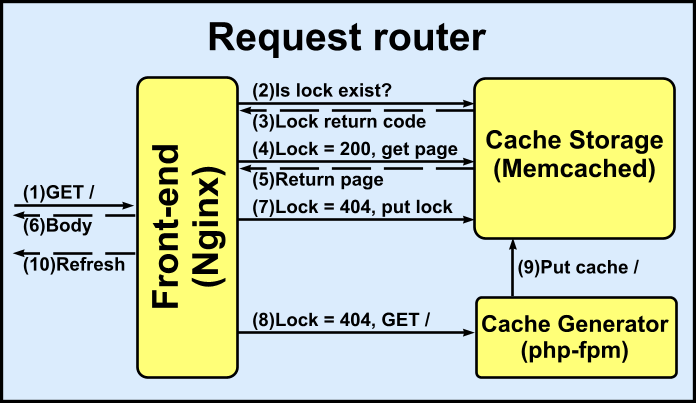
\includegraphics[width=8cm]{14_kraev.png}}
\label{pic:kraev}
%\caption{Приложения по категориям}
\end{figure}

По этой схеме Nginx выступает в качестве маршрутизатора между хранилищем кэша и кэш-генератором, вызывая для обработки запросов LUA-скрипт. Таким образом, страницы всегда отдаются из кэша. Если же кэша не существует, отправляется запрос для его генерации, а клиент перенаправляется на refresh-страницу, которая заставляет отправить запрос повторно через заданное время. Кэш имеет expire time = 0, что означает,  что он никогда не будет удален. Для обновления кэша используется lock с ограниченным expire time (в зависимости от запрашиваемой страницы), и когда expire time истекает "--- кэш регенерируется и помещается поверх старого. Также lock имеет еще одну важную функцию: его наличие предотвращает отправку запросов на генерацию из других фронтендов, если  автомасштабируемый кластер стал раздуваться, и в группе находится больше одного инстанса. 

Общее хранилище решает проблему прегенерации кэша. Так, при добавлении нового инстанса, он сразу вступает в распределение нагрузки, используя кэш из общего хранилища.  Такой подход позволяет ускорить ресурсы не только с Wordpress, а в принципе любой ресурс с ПО, написанным на любом коде, из которого генерируется HTML.

\section*{Save and profit!}

Использование данных технологий позволило нашей компании существенно снизить затраты на техническое обеспечение интернет-ресурса \url{theuptake.org}. Заменив 8 физических серверов (80--90\% времени они простаивали, но были необходимы из-за периодических резких всплесков посещений после публикации новостей), на 1 large-инстанс, на котором хранится общий контент и кэш, 1 RDS-инстанс, в котором лежит БД и автомасштабируемая группировка, работающая во время простоя с 1 smallинстанса и раздуваемая до кластера, размер которого определяет нагрузка. В дополнение к экономии (т.к. сегодня мы платим только за пики) мы многократно повысили скорость отдачи контента,  доступность и отказоустойчивость ресурса. 

\end{document}

%\documentclass[10pt, a5paper]{article}
\usepackage{ucs}
\usepackage[utf8]{inputenc}
\usepackage[T2A]{fontenc}
\usepackage[english, russian]{babel}
\usepackage{hyperref}
\usepackage{geometry}
\frenchspacing

\begin{document}

\title{Способы повышения производительности высоконагруженных проектов на CMS Drupal}

\author{Виталий Иоскевич\footnote{Минск, Беларусь}}
\date{}
\maketitle
\renewcommand{\abstractname}{Abstract}
\begin{abstract}
Drupal is a popular CMS/CMF used to power the different types of web-projects worldwide. The desire of developers to make their system competitive in terms of functionality and flexibility sooner or later leads to increase of server load and reduced performance. Extensive functionality, flexibility in configuration and extensibility through third-party modules are undoubtedly a huge advantage, enabling to carry out projects of varying complexity and purpose, but the price often is a poor performance of high loaded Drupal-powered sites.
In our review we are going to revise existing standard methods of Drupal performance optimization (both server- and client-side) and demonstrate custom solutions that can be applied to some of the critical areas of Drupal-powered high-loaded web-site. In our real-life example we are going to show how to build Google Map page, capable to show thousands of markers based on Drupal content nodes.*

Насчет изменения предложения - "/Кэширование критично как для анонимов, так и для авторизованных пользователей. Используется Pressflow/Varnish/" - нет проблем. 
\end{abstract}
  
Drupal (7-ая, текущая версия) является достаточно развитой системой управления контентом. Стремление разработчиков сделать свою систему универсальной и более функциональной, чем у конкурентов, рано или поздно приводит к тому, что возрастают нагрузки на сервер, снижается быстродействие. Обширный функционал, гибкость в конфигурировании и расширяемость посредством сторонних модулей несомненно являются огромным преимуществом, благодаря которому позволяет выполнять проекты различной сложности и назначения, но плата за него --- низкая производительность готового решения. 

Чем больше число использованных на сайте сторонних модулей (в т.~ч. собственной разработки), тем ниже производительность сайта при больших нагрузках (большом количестве посетителей), а именно при построении сайтов с предполагаемым большим числом  посетителей никак не обойтись стандартным функционалом CMS. Таким образом, данная CMS оказывается весьма требовательной к ресурсам сервера, и в большинстве случаев проблема  решается выбором специализированных дорогих хостингов --- выделенный сервер или несколько серверов. 

Но и при ограниченных возможностях сервера есть способы улучшения производительности сайта. Стандартной системы кэширования Drupal достаточно для нормальной работы среднего сайта при неинтенсивной посещаемости, однако для случая высокой нагрузки на сайт этой системы недостаточно.

\section*{Основные методы повышения производительности Drupal:}
\begin{itemize}
	\item включить кэш в модулях, позволяющих кэширование (таких как Views, Panels, Feeds, SWF Tools и т.п.);
	\item увеличить время жизни кэша для стандартной системы кэширования Drupal. При этом надо иметь ввиду, что посетители будут видеть обновления содержимого значительно позже;
	\item если нет большой необходимости в статистике, можно выключить стандартные модули statistics и database logging. Они используют дополнительные запросы к БД при загрузке страницы. Кроме того, можно найти альтернативу данным модулям;
	\item использовать модуль CSS Gzip. Уменьшает размер файлов и количество http-запросов;
	\item использовать модуль Global Redirect. Предотвращает кэширование дубликатов содержимого сайта по ссылкам псевдонимам (синонимам) в случае использования <<Clean URL>>;
	\item использовать модуль Javascript Aggregator. Настройки Drupal позволяют объединить js-файлы, однако этот модуль позволяет еще и уменьшить конечный размер передаваемого файла;
	\item заменить системный cron на более функциональный модуль Elysia Cron. В отличие от системного, Elysia Cron позволяет распределить задачи по времени одна за одной, а не все вместе, при этом снижая пиковую нагрузку на сервер;
	\item перенести вызов javascript вниз станицы;
	\item помещать сторонние библиотеки вне каталога модулей /sites/all/modules --- например, в /sites/all/libraries. В таком случае Drupal не будет просматривать ненужные ему файлы;
	\item конвертировать таблицы MySQL в UTF8 InnoDB;
	\item создать индексы для медленных запросов Views. Желательно проанализировать такие запросы и увеличить производительность созданием индексов для полей;
	\item использовать ImageMagick вместо стандартной GD image library, т.~к. он лучше использует ресурсы сервера и дает лучшее качество изображений;
	\item использовать модуль Content Delivery Network integration. Он позволяет распределить файлы на множество отделенных друг от друга серверов. При этом снижается динамическая нагрузка на сервер, но требуется дополнительная плата за каждый сервер;
\end{itemize}

Наиболее продуктивным способом увеличения производительности является использование отдельной  эффективной системы кэширования.

{\bf Boost}. Одна из лучших систем кэширования для shared hosts. Cоздает копии html-станиц, которые генерирует Drupal, и хранит их в каталоге cache. Используя правила <<.htaccess>>, Boost проверяет, существует ли необходимый файл. Если да, то загружает статичный html, полностью избегая Drupal/PHP/MySQL. Если нет,  генерирует файл. Старые файлы удаляются по cron для того, чтобы выводимое содержимое сайта оставалось свежим (актуальным).

{\bf Memcache}. Серверная система кэширования, сохраняющая страницы сайта в оперативной памяти сервера. Все что необходимо для эффективной работы в данном случае --- быстрое ОЗУ большого объема. Его можно успешно использовать как для кэширования анонимных пользователей, так и для зарегистрированных. Но возможен и вариант, когда Memcache кэширует зарегистрированных пользователей, а Boost используется для кэширования анонимов. К преимуществам варианта можно отнести возможность кэширования анонимов и зарегистрированных пользователей, а к недостаткам --- то, что нужен хотя бы VPS, c достаточной оперативной памятью и невозможность работы на shared hosting.

{\bf APC(Alternate PHP Cache)}. Система кэширования op-code для серверов Apache. Подход весьма эффективен при большом числе активных модулей на сайте. Суть системы заключается в кэшировании компилированного байт-кода PHP-скрипта для того, чтобы избежать расходов ресурсов сервера на разбор и компиляцию исходного кода при каждом запросе. Для дальнейшего повышения производительности кэшированный код хранится в общей памяти и непосредственно выполняется оттуда, тем самым сводя к минимуму количество медленных операций чтения файлов и копирования в памяти во время выполнения.
К преимуществам относится ускорение компиляции скриптов Drupal и уменьшение использования ресурсов сервера, к недостаткам --- необходимость произвести специальное конфигурирование сервера.

{\bf Varnish(reverse proxy http-accelerator)}. Данная система выступает на первом плане над сервером Apache, PHP и Drupal. Varnish сохраняет кэшированное содержимое в оперативной памяти, и таким образом экономит ресурсы на загрузке Apache и Drupal. В результате этого Varnish предоставляет высокую производительность для кэшированных страниц для анонимных пользователей и является предпочтительным вариантом для сложных ресурсоемких сайтов, требующих значительной  масштабируемости. Для работы с Drupal 6 необходима была отдельная <<оптимизированная>> сборка дистрибутива под названием PressFlow и установка модуля интеграции Varnish HTTP Accelerator Integration. Для текущей версии Drupal достаточно установки модуля.

\section*{Пример проекта с высокой нагрузкой --- 350.org (Drupal 6)}

К характеристикам проекта можно отнести следующие: 
\begin{itemize}
	\item 150 000+  уникальных посетителей в день
	\item 6000+ ивентов, созданных пользователями
	\item ~500 авторизованных пользователей в среднем постоянно на сайте
	\item Самая посещаемая страница: карта ивентов (/map)
\end{itemize}

Кэширование критично как для анонимов, так и для авторизованных пользователей. Используется Pressflow/Varnish

Cпециальные меры и собственные разработки для повышения производительности включают:
\begin{itemize}
	\item Отказ от Views для генерации больших массивов данных
	\item  XML файл на диск вместо DB кэш (плюсы/минусы)
	\item Кэширование на диск всех RSS фидов
	\item Ajax запросы информации для маркеров на карте
\end{itemize}

\end{document}





%\documentclass[10pt, a5paper]{article}
\usepackage{pdfpages}
\usepackage{parallel}
\usepackage[T2A]{fontenc}
\usepackage{ucs}
\usepackage[utf8x]{inputenc}
\usepackage[polish,english,russian]{babel}
\usepackage{hyperref}
\usepackage{rotating}
\usepackage[inner=2cm,top=1.8cm,outer=2cm,bottom=2.3cm,nohead]{geometry}
\usepackage{listings}
\usepackage{graphicx}
\usepackage{wrapfig}
\usepackage{longtable}
\usepackage{indentfirst}
\usepackage{array}
\newcolumntype{P}[1]{>{\raggedright\arraybackslash}p{#1}}
\frenchspacing
\usepackage{fixltx2e} %text sub- and superscripts
\usepackage{icomma} % коскі ў матэматычным рэжыме
\PreloadUnicodePage{4}

\newcommand{\longpage}{\enlargethispage{\baselineskip}}
\newcommand{\shortpage}{\enlargethispage{-\baselineskip}}

\def\switchlang#1{\expandafter\csname switchlang#1\endcsname}
\def\switchlangbe{
\let\saverefname=\refname%
\def\refname{Літаратура}%
\def\figurename{Іл.}%
}
\def\switchlangen{
\let\saverefname=\refname%
\def\refname{References}%
\def\figurename{Fig.}%
}
\def\switchlangru{
\let\saverefname=\refname%
\let\savefigurename=\figurename%
\def\refname{Литература}%
\def\figurename{Рис.}%
}

\hyphenation{admi-ni-stra-tive}
\hyphenation{ex-pe-ri-ence}
\hyphenation{fle-xi-bi-li-ty}
\hyphenation{Py-thon}
\hyphenation{ma-the-ma-ti-cal}
\hyphenation{re-ported}
\hyphenation{imp-le-menta-tions}
\hyphenation{pro-vides}
\hyphenation{en-gi-neering}
\hyphenation{com-pa-ti-bi-li-ty}
\hyphenation{im-pos-sible}
\hyphenation{desk-top}
\hyphenation{elec-tro-nic}
\hyphenation{com-pa-ny}
\hyphenation{de-ve-lop-ment}
\hyphenation{de-ve-loping}
\hyphenation{de-ve-lop}
\hyphenation{da-ta-ba-se}
\hyphenation{plat-forms}
\hyphenation{or-ga-ni-za-tion}
\hyphenation{pro-gramming}
\hyphenation{in-stru-ments}
\hyphenation{Li-nux}
\hyphenation{sour-ce}
\hyphenation{en-vi-ron-ment}
\hyphenation{Te-le-pathy}
\hyphenation{Li-nux-ov-ka}
\hyphenation{Open-BSD}
\hyphenation{Free-BSD}
\hyphenation{men-ti-on-ed}
\hyphenation{app-li-ca-tion}

\def\progref!#1!{\texttt{#1}}
\renewcommand{\arraystretch}{2} %Іначай формулы ў матрыцы зліпаюцца з лініямі
\usepackage{array}

\def\interview #1 (#2), #3, #4, #5\par{

\section[#1, #3, #4]{#1 -- #3, #4}
\def\qname{LVEE}
\def\aname{#1}
\def\q ##1\par{{\noindent \bf \qname: ##1 }\par}
\def\a{{\noindent \bf \aname: } \def\qname{L}\def\aname{#2}}
}

\def\interview* #1 (#2), #3, #4, #5\par{

\section*{#1\\{\small\rm #3, #4. #5}}

\def\qname{LVEE}
\def\aname{#1}
\def\q ##1\par{{\noindent \bf \qname: ##1 }\par}
\def\a{{\noindent \bf \aname: } \def\qname{L}\def\aname{#2}}
}

\begin{document}
\title{Открытые протоколы --- основа распределенных социальных сетей}
\author{Александр Загацкий\footnote{Витебск, Беларусь, \url{http://zag.ru}, \url{me@zag.ru}}}
\date{}
\maketitle

\begin{abstract}Distributed networks help users to control their online identity in the Internet.
Their key feature is absence of a central server. Nodes
in the network belong to each one of its
participants, and software runs on user's computer
or on trusted server. User determines the distribution policy
of his data.
Distributed social networks are built upon open technologies, such as Atom,
WebFinder, OpenID/OAuth, Salmon, ActivityStreams and etc.
Most of developed distributed networks are opensourced and under
development. Some of them are available to use, i.e. 
SatausNet --- the open source microblogging platform that
helps you share and connect in real-time within your own domain. Yet
another distibuted social network OneSocialWeb is a dream of the world where
all social networks are connected and work together similar
to email.
\end{abstract}
Весной этого года в одном из дата-центров провайдера облачного хостинга
Amazon EC2 произошел сбой \cite{zag1}, в результате чего перестали
 функционировать такие сервисы как Friendfeed, Quora, Reddit, Hootsuite,
 foursquare. По неожиданной случайности это совпало с началом судного дня
 в сериале "Терминатор: Битва за будущее". По сюжету фильма в этот день
 военная компьютерная сеть SkyNet, управляющая военными роботами вышла из
 под контроля человека и произвела ряд ядерных атак на человечество. К
 каким последствиям может привести утрата контроля над персональными
 данными, созданными пользователями в сети и раскрывающие отдельные
 моменты их личной жизни?

 Этот случай заставил задуматься о надежности социальных сервисов и
 сохранности пользовательских данных. Помимо этого за социальными
 сервисами стоят организации. Как следствие, функционирование сервиса
 зависит зачатую от материального положения владельца сервиса. Таким
 образом, сохранность личных данных и контроль над доступом к ним являются
 актуальной задачей для пользователей Интернет.

 Отчасти решить очерченную задачу призваны децентрализованные
 (распределенные) социальные сети. Характерной их особенностью, является
 отсутствие центрального сервера. Узлы сети принадлежат каждому из ее
 участников, а программное обеспечение функционирует на компьютере
 пользователя или на доверенном сервере. При этом пользователь
 самостоятельно определяет политику распространения его данных.

 В основе функционирования распределенных сетей лежат открытые протоколы.
 Ключевыми из них являются следующие:

 \subsubsection*{Atom/RSS}
% \begin{figure}[ht]
%\centering{
\includegraphics{16_zag1_atom-logo.png}}
%\end{figure}

    Формат синдикации Atom основан на XML и позволяет описывать наборы
    веб-ресурсов. Например: новостные ленты, анонсы статей в блоге,
    галереи фотографий и тому подобное. Формат описан в RFC 4287 \cite{zag2}.

    \subsubsection*{XRD}
 Стандарт описания ресурса доступен в \cite{zag3}. Представляет собой
    последовательное описание данных аккаунта в формате XML. Среди
    данных --- сведения о серверах аутентификации, публичные криптоключи и т.д.

    \subsubsection*{WebFinder}
% \begin{figure}[ht]
%\centering{
\includegraphics{16_zag1_WebFinger.png}}
%\end{figure}
    Протокол, позволяющий идентифицироваться пользователю. В качестве
    идентификации используется запись вида 
    
    \verb!acct:joe@example.com!

    По данному адресу устанавливается сервер с учетной записью
    пользователя и извлекаются XRD-записи.

 \subsubsection*{OpenID/OAuth}
%  \begin{figure}[ht]
%\centering{
\includegraphics{16_zag1_penid-icon.png}}
%\end{figure}
    Протоколы аутентификации и авторизации. Позволяют повысить
    безопасность при взаимодействии нескольких независимых сервисов.

    \subsubsection*{Pubsubhubbub}
%   \begin{figure}[ht]
%\centering{
\includegraphics{16_zag1_pubsubhubbub.png}}
%\end{figure}
    Протокол позволяет сообщать об обновлениях другим ресурсам. При этом
    используются так называемые хабы, которые сообщают об изменениях на
    основном ресурсе подписчикам. Такая схема позволяет реализовать 
    Push-канал обновлений, снизив нагрузку на источник изменений.

    Авторами являются сотрудники Google: Brad Fitzpatrick and Brett
    Slatkin. Источник обновления децентрализуется. Адрес hub для
    обновлений указывается в RSS/Atom в следующем формате:

\noindent     \verb!<link rel="hub" href="http://myhub.example.com/endpoint"/>!


     \subsubsection*{Salmon}
%    \begin{figure}[ht]
%\centering{
\includegraphics{16_zag1_customLogo.png}}
%\end{figure}
    Этот протокол позволяет отправлять действия по отношению к объекту
    (например, статье или заметке) с агрегаторов в оригинальный
    источник. Например, Salmon используется для сбора комментариев к
    оригинальной статье с других сайтов, на которых статья была
    опубликована.

    Адрес для отправки обновлений указан в RSS/Atom:

\noindent        \verb!<link rel="salmon"! \linebreak
\verb!href="http://example.org/salmon-endpoint"/>!

    Особенностью данного протокола является крипто-подпись сообщений,
    которая позволяет решить проблемы со спамом. Для получения
    публичного ключа используется формат XRD.

    \subsubsection*{ActivityStreams}
%    \begin{figure}[ht]
%\centering{
\includegraphics{16_zag1_icon-lg.png}}
%\end{figure}
    Формат описания активности пользователя на ресурсах. Благодаря этому
    формату происходит уведомление узлов распределенной сети о действиях
    пользователей: написании комментария, выставление оценки <<нравится>>,
    публикации фотографий и т.д. Из форматов доступны как JSON, так и
    расширения Atom \cite{zag4}.

    \subsubsection*{XMPP}
    Протокол обмена XMPP (<<Jabber>>) лежит в основе транспорта между
    узлами нескольких распределенных сетей. В качестве клиента
    используется как десктопные программы, так и мобильные версии.

    \subsubsection*{Portable Contacts}
    Протокол безопасного предоставления данных о своих контактах внешним
    сервисам \cite{zag5}. При этом используется протокол OAuth, и
    пользователь управляет доступом к своему списку контактов.

 Среди проектов создания распределенных социальных сетей \linebreak можно отметить
 следующие:
 \begin{description}
	 \item[StatusNet] \cite{zag6}\\
   Открытую платформу для микроблоггинга (аналог Twitter) StatusNet
    можно установить на собственном домене. Платформа предназначена для
    коллективного использования. Лицензия: AGPLv3.
    \item[GNU Social] \cite{zag7}\\
    Соответствует философии Unix: маленькие программы делают маленькие
    работы. По возможностям близка к Status.net: микроблоггинг. Лицензия:
    AGPLv3.
    \item[Diaspora] \cite{zag8}\\
    Проект Diaspora, созданный по инициативе четырех студентов,
    предназначен для персонального использования: ведения микроблога,
    публикации фотографий. Лицензия: AGPL-3.0.
    \item[friendika] \cite{zag9}\\
    Возможности: cервер профилей и поддержка ряда других сетей
    (Diaspora, Google Buzz, Identi.ca, Twitter), поддержка \linebreak шифрования
    между серверами. Лицензия: BSD License.
    \item[OneSocialWeb] \cite{zag10}
    Данная сеть микроблоггинга использует в качестве транспорта протокол
    XMPP \cite{zag11}. В качестве идентификатора пользователя
    используется jabber ID, часть протоколов адаптирована для
    использования в Jabber-сети. Лицензия: Apache 2.
\end{description}
 Это небольшая часть из разрабатываемых проектов, позволяющих
 пользователю сети управлять своими данными и быть независимым в контроле
 над персональной информацией. Тем не менее, очевидно, что персональные
 данные являются основной составляющей социальной жизни в сети и
 определять политику их использования может только пользователь.
\begin{thebibliography}{99}
	\bibitem{zag1} "Судный день для моих персональных данных". \url{http://zag.ru/a4BR2}
	\bibitem{zag2} RFC 4287: The Atom Syndication Format. \url{http://tools.ietf.org/html/rfc4287}
	\bibitem{zag3} Extensible Resource Descriptor (XRD). \url{http://docs.oasis-open.org/xri/xrd/v1.0/xrd-1.0.html}
	\bibitem{zag4} Формат оповещений Activity Streams. \url{http://activitystrea.ms/}
	\bibitem{zag5} Протокол Portable Contacts. \url{http://code.google.com/intl/ru-RU/apis/contacts/docs/poco/1.0/developers_guide.html}
	\bibitem{zag6} Платформа для микроблоггинга StatusNet. \url{http://status.net/}
	\bibitem{zag7} Распределенная сеть GNU Social. \url{http://foocorp.org/projects/social/}
	\bibitem{zag8} Социальная сеть Diaspora. \url{http://www.joindiaspora.com/}
	\bibitem{zag9} Распределенная сеть Friendika. \url{http://project.friendika.com}
	\bibitem{zag10} Социальная сеть OneSocialWeb, построенная на основе протокола XMPP. \url{http://onesocialweb.org/}
	\bibitem{zag11} XMPP - открытый протокол обмена сообщениями и информацией о статусе. \url{http://ru.wikipedia.org/wiki/XMPP}
\end{thebibliography}

\end{document}

%\documentclass[10pt, a5paper]{article}
\usepackage{ucs}
\usepackage[utf8]{inputenc}
\usepackage[T2A]{fontenc}
\usepackage[english, russian]{babel}
\usepackage{hyperref}
\usepackage{geometry}
\usepackage{listings}
\frenchspacing
\begin{document}
\title{Perl 6 Pod --- формат ведения документации}
\author{Александр Загацкий\footnote{Витебск, Беларусь, \url{http://zag.ru}, \url{me@zag.ru}}}
\date{}
\maketitle

\begin{abstract}
Pod is an evolution of Perl 5's POD markup. Compared to POD, Perl 6's
Pod is much more
uniform, somewhat more compact, and considerably more
expressive. Established in 2005, specification
has undergone several revisions and is currently stable. The
specification is written in Perl 6 Pod and is a
good means of testing the implementations.
There are several implementations in Perl 5 and Perl 6.
Presentation covers the differences from Perl 5 POD, key features and 
experience of Perl 6 Pod personal usage.
\end{abstract}

Формат разметки Perl 6 Pod перестал быть черновиком. В финальной версии
спецификации Synopsis 26 \cite{zag1pod} добавился ряд особенностей.
Никогда не еще не было настолько тесной интеграции программного кода и
документации к нему.

Так, добавился специальный тип блоков документации --- блоки-деклараторы.
Данные блоки предваряются специальным комментарием \verb!#=!, за которым
следует текст документации. Оформленные блоки документации ассоциируются
с делараторами подпрограмм, а так же переменных. Уникальной особенностью
является тот факт, что эти блоки документации становятся доступными
через специальный атрибут \verb!.WHY!. Например:

\begin{lstlisting}[language={Perl}]
 sub fu (           #= This text stored in &fu.WHY
  Any     $bar,    #= This text stored in $bar.WHY
  Mode    :$baz   #= This text stored in $baz.WHY
    ) { ... }

 #= This is a special chainsaw
 my SwissArmy $chainsaw    #= (It has a rocket launcher)

 say $chainsaw.WHY; # prints: This is a special chainsaw
                   #         (It has a rocket launcher)
\end{lstlisting}


В приведенном примере текст документации к переменной \verb!$chainsaw!
становится доступным из программного кода. В указанном примере блок кода
будет выведен на экран:
\begin{lstlisting}[language={Perl}]
 say $chainsaw.WHY; # prints: This is a special chainsaw
                   #         (It has a rocket launcher)
\end{lstlisting}

Уникальна сама концепция, а именно доступ программного кода к
документации по нему. То есть становится возможным менять логику
программы в зависимости от описанной в документации!

Еще одним примером интеграции документации и кода являются
контекстуальные псевдонимы. Для их определения используется директива
\verb!=alias!. Например:
\begin{lstlisting}[language={Perl}]
 # This is actual code...
 sub hash_function ($key)
 *=alias HASHCODE*
 {
    my $hash = 0;
    for $key.split("") -> $char {
        $hash = $hash*33 + $char.ord;
    }
    return $hash;
 }
	   \end{lstlisting}

В данном примере определяется псевдоним HASHCODE. Его значением
является следующий за ним программный блок. Теперь, чтобы привести в
документации пример кода достаточно указать имя псевдонима внутри кода
форматирования \verb!A<>!:
\begin{lstlisting}[language={Perl}]
 =begin pod
 An ancient (but fast) hashing algorithm is used:
 =begin code :allow<A>
  A<HASHCODE>
 =end code
 =end pod
\end{lstlisting}

В результате в документации будет вставлен блок кода из программы:
\begin{lstlisting}[language={Perl}]
 An ancient (but fast) hashing algorithm is used:

    my $hash = 0;
    for $key.split("") -> $char {
        $hash *= 33;
        $hash += $char.ord;
    }
    return $hash;
	   \end{lstlisting}

Это позволяет избежать ручного копирования блоков кода и последующую
актуализацию документации.


\begin{thebibliography}{9}
	\bibitem{zag1pod} Спецификация формата Pod (Synopsis 26). \url{https://github.com/zag/specs/raw/master/S26-documentation.pod}
\end{thebibliography}

\end{document}

%\documentclass[10pt, a5paper]{article}
\usepackage{ucs}
\usepackage[utf8]{inputenc}
\usepackage[T2A]{fontenc}
\usepackage[english, russian]{babel}
\usepackage{hyperref}
\usepackage{geometry}
\frenchspacing

\begin{document}

\title{LeechCraft: открытый модульный интернет-клиент}

\author{Рудой Г. И.\footnote{Московский физико-технический институт, \url{0xd34df00d@gmail.com}}, Линкин О. Е.\footnote{Министерство Обороны Республики Беларусь, MaledictusDeMagog@gmail.com}}
\date{}
\maketitle

\begin{abstract}
LeechCraft, the open source modular
cross-platform internet client written in C++/Qt, is reviewed mostly from the
technical perspective. Design decisions are described as far as solutions of
the problems faced during development and arising from the modular
nature of the application. Other aspects of open development are also
briefly considered, such as building a community or future goals. 
The paper should be of high interest to those developing highly modular
applications or general open source projects.
\end{abstract}

LeechCraft --- это открытый модульный кросс-платформенный
интернет-клиент. LeechCraft ориентирован на выполнение типичных
пользовательских задач, связанных с интернетом, в том числе:
\begin{itemize}
	\item просмотр веб-страниц;
	\item чтение лент новостей;
	\item скачивание файлов;
	\item обмен мгновенными сообщениями. 
\end{itemize}
В то же время реализованы и другие функции: например, менеджер
пакетов, работающий в пространстве пользователя, простой текстовый
редактор, медиа-плеер.

Модульность приложения означает, что все задачи в LeechCraft
выполняются загружаемыми модулями, которые при желании можно отключать
либо не устанавливать. Модули также могут взаимодействовать друг с
другом: например, модуль для чтения лент новостей использует модуль
поддержки протокола HTTP для скачивания этих лент. Ядро приложения при
этом обеспечивает лишь загрузку модулей, корректный порядок их
инициализации, обеспечивает их взаимное взаимодействие и предоставляет
некоторые базовые сервисы, например, сетевой кэш или базу данных
cookies.

Среди преимуществ такой архитектуры со слабо зависящими друг от друга
(а именно, от конкретной реализации) модулями можно отметить высокую
гибкость приложения, значительное снижение дублирования
функциональности и кодо-расширяемость, возможность заменять модули на
другие, выполняющие аналогичные функции, без изменения кода вне этих
модулей, и т.~д. Так, например, модуль поддержки скриптовых плагинов
позволяет произвольному модулю взаимодействовать со скриптами, даже
если этот модуль не имеет никакой прямой поддержки скриптинга.

Одним из выбранных способов реализации такой архитектуры является
взаимодействие модулей при помощи обмена сообщениями --- специальными
структурами данных с заданными правилами обработки. Один модуль
посылает сообщение по соответствующей шине приложения, а ряд других
модулей опрашивается на предмет возможности обработки этого сообщения,
и каждый из этих модулей может во время выполнения либо обработать
сообщение, либо отказаться от его обработки.

В то же время иногда необходимо тесное связывание модулей друг с
другом. Например, модуль блокировки рекламы в веб-браузере тесно
связан с самой реализацией браузера, и сделать его абстрагированным от
конкретного модуля браузера не представляется возможным, а система
поддержки стилей чатов в клиенте мгновенных сообщений связана с
реализацией самого IM-клиента. Для таких случаев обеспечивается
возможность прямого соединения модулей друг с другом (при этом один из
модулей считается плагином для другого модуля), а модули сами
определяют удобный им протокол взаимодействия.

Однако, помимо упомянутых преимуществ, поставленная задача
реализации конечной функциональности при помощи слабо зависящих друг
от друга модулей создает ряд проблем, часть из которых связана со
статичной природой выбранного языка реализации (C++) и отсутствием в
нем полноценной поддержки RTTI и какого-либо Reflection. Например, при
реализации вышеупомянутого модуля поддержки скриптовых плагинов
необходима возможность во время выполнения приложения определять
используемые другими модулями протоколы взаимодействия друг с другом,
так как прямое добавление информации о соответствующих протоколах на
этапе написания кода либо на этапе компиляции противоречит принципу
слабого связывания. Возможности интроспекции, предоставляемые
фреймворком Qt, позволяют успешно решить эту проблему при условии
соблюдения простых правил при написании модулей.

Другие вопросы, возникающие при разработке подобных приложений --- это
создание сообщества вокруг приложения и его общее позиционирование.
Социальный аспект открытой разработки является не менее важным, чем
технический, поэтому он также обсуждается в докладе.

\begin{thebibliography}{9}
	\bibitem{leechcraft1} LeechCraft Architecture --- \url{http://leechcraft.org/development-leechcraft-architecture}
	\bibitem{leechcraft2} Gamma et al. Design Patterns: Elements of Reusable Object-Oriented Software. Addison-Wesley, 1995
\end{thebibliography}


\end{document}





%\documentclass[10pt, a5paper]{article}
\usepackage{pdfpages}
\usepackage{parallel}
\usepackage[T2A]{fontenc}
\usepackage{ucs}
\usepackage[utf8x]{inputenc}
\usepackage[polish,english,russian]{babel}
\usepackage{hyperref}
\usepackage{rotating}
\usepackage[inner=2cm,top=1.8cm,outer=2cm,bottom=2.3cm,nohead]{geometry}
\usepackage{listings}
\usepackage{graphicx}
\usepackage{wrapfig}
\usepackage{longtable}
\usepackage{indentfirst}
\usepackage{array}
\newcolumntype{P}[1]{>{\raggedright\arraybackslash}p{#1}}
\frenchspacing
\usepackage{fixltx2e} %text sub- and superscripts
\usepackage{icomma} % коскі ў матэматычным рэжыме
\PreloadUnicodePage{4}

\newcommand{\longpage}{\enlargethispage{\baselineskip}}
\newcommand{\shortpage}{\enlargethispage{-\baselineskip}}

\def\switchlang#1{\expandafter\csname switchlang#1\endcsname}
\def\switchlangbe{
\let\saverefname=\refname%
\def\refname{Літаратура}%
\def\figurename{Іл.}%
}
\def\switchlangen{
\let\saverefname=\refname%
\def\refname{References}%
\def\figurename{Fig.}%
}
\def\switchlangru{
\let\saverefname=\refname%
\let\savefigurename=\figurename%
\def\refname{Литература}%
\def\figurename{Рис.}%
}

\hyphenation{admi-ni-stra-tive}
\hyphenation{ex-pe-ri-ence}
\hyphenation{fle-xi-bi-li-ty}
\hyphenation{Py-thon}
\hyphenation{ma-the-ma-ti-cal}
\hyphenation{re-ported}
\hyphenation{imp-le-menta-tions}
\hyphenation{pro-vides}
\hyphenation{en-gi-neering}
\hyphenation{com-pa-ti-bi-li-ty}
\hyphenation{im-pos-sible}
\hyphenation{desk-top}
\hyphenation{elec-tro-nic}
\hyphenation{com-pa-ny}
\hyphenation{de-ve-lop-ment}
\hyphenation{de-ve-loping}
\hyphenation{de-ve-lop}
\hyphenation{da-ta-ba-se}
\hyphenation{plat-forms}
\hyphenation{or-ga-ni-za-tion}
\hyphenation{pro-gramming}
\hyphenation{in-stru-ments}
\hyphenation{Li-nux}
\hyphenation{sour-ce}
\hyphenation{en-vi-ron-ment}
\hyphenation{Te-le-pathy}
\hyphenation{Li-nux-ov-ka}
\hyphenation{Open-BSD}
\hyphenation{Free-BSD}
\hyphenation{men-ti-on-ed}
\hyphenation{app-li-ca-tion}

\def\progref!#1!{\texttt{#1}}
\renewcommand{\arraystretch}{2} %Іначай формулы ў матрыцы зліпаюцца з лініямі
\usepackage{array}

\def\interview #1 (#2), #3, #4, #5\par{

\section[#1, #3, #4]{#1 -- #3, #4}
\def\qname{LVEE}
\def\aname{#1}
\def\q ##1\par{{\noindent \bf \qname: ##1 }\par}
\def\a{{\noindent \bf \aname: } \def\qname{L}\def\aname{#2}}
}

\def\interview* #1 (#2), #3, #4, #5\par{

\section*{#1\\{\small\rm #3, #4. #5}}

\def\qname{LVEE}
\def\aname{#1}
\def\q ##1\par{{\noindent \bf \qname: ##1 }\par}
\def\a{{\noindent \bf \aname: } \def\qname{L}\def\aname{#2}}
}


\begin{document}
\title{Создание специализированного дистрибутива Linux для подключения к национальной GRID-сети}
\author{Денис Пынькин\footnote{Минск, Беларусь}}
\def\progref!#1!{\texttt{#1}}

\maketitle

\begin{abstract}
Unicore is ready"=to"=run system used as main platform for belarussian national GRID network. 
There are no Linux distributions for bare-metal Unicore installation and user"=friendly administration. 
Article describes steps to produce Linux server based on ALTLinux technologies with Unicore services working out of the box.
\end{abstract}

\section*{Сборка базового дистрибутива}
Современные дистрибутивы ALT Linux собираются с помощью инструмента mkimage,
который состоит из набора правил для утилиты make и вспомогательных скриптов 
и предоставляет базовый функционал для сборки образа Linux-системы. 
Фактически для создания своего собственного дистрибутива достаточно в 
правильном порядке и с правильными параметрами собрать из предоставляемых 
<<кирпичиков>> единое целое, что в общем-то является нетривиальной задачей.

Так было предпринято несколько попыток создать универсальные профили для mkimage,
но наиболее удачным и развитым оказался mkimage-profiles-desktop 
(в рассылках и на форумах часто сокращают до аббревиатуры M-P-D).

Далее, на примере создания дистрибутива Unicore для упрощения подключения к 
белорусской национальной научной GRID-сети, описывается как можно 
использовать M-P-D для создания собственного инсталляционного образа сервера.

Для начала необходимо получить правила сборки дистрибутива из git-репозитория:
\begin{verbatim}
git clone git://git.altlinux.org/people/boyarsh/packages/
 mkimage-profiles-desktop
\end{verbatim}

 Создать файл для пакетного менеджера apt с описанием репозитория и соответствующей 
 архитектурой, который необходимо расположить по пути {\tt \~/\$branch-\$arch.conf}, 
 в случае стабильного репозитория для Platform 6 и 64-битной архитектуры "--- \linebreak 
 {\tt \~/p6-x86\_64.conf}. В качестве минимума в этом файле должна содержаться 
 ссылка на файл с описаниями источников пакетов, для нашего примера "---
 {\tt \~/p6-sources-x86\_64.list}.

Например для белорусского зеркала ALT Linux эти файлы будут выглядеть следующим образом:

{\tt p6-x86\_64.conf}:
\begin{verbatim}
Dir::Etc::SourceList "/home/d4s/p6-sources-x86\_64.list";
\end{verbatim}

{\tt p6-sources-x86\_64.list}:
\begin{verbatim}
rpm [p6] ftp://ftp.mgts.by/pub/ALTLinux/p6/branch x86_64
 classic
rpm [p6] ftp://ftp.mgts.by/pub/ALTLinux/p6/branch noarch
 classic
\end{verbatim}

Для создания установочного диска своего сервера удобнее всего использовать 
профиль от Антона Фарыгина, который можно собрать в качестве теста, 
чтобы проверить работоспособность конфигурации. 
Например, таким образом можно собрать установочный диск для 64-битной 
архитектуры с дизайном Sisyphus:
\begin{verbatim}
archs=x86_64 ./make-distro server-light
 --with-branding=altlinux-sisyphus
\end{verbatim}

На консоль ничего не выводится, но это не страшно "--- <<все ходы записаны>>, 
а ход сборки протоколируется в файлы вида \linebreak <target>.<arch>.log или, в нашем 
случае, в файл \linebreak {\tt server-light.x86\_64.log}.

Получившийся образ диска сохраняется в домашнем каталоге {\tt ~/out/<target>} ({\tt ~/out/server-light/}).

Теперь можно приступать к созданию собственного сервера.

\section*{Модификация базового дистрибутива}
Модификация базового дистрибутива проводится с помощью дополнительных пакетов 
и изменения M-P-D для добавления своих правил сборки дистрибутива и 
списков программного обеспечения, которое будет доступно во время и после установки.

Все дополнительные пакеты условно можно разбить на две категории "--- функциональные и вспомогательные.

К функциональным относятся пакеты, которые содержат все необходимое для 
полноценного выполнения сервером той задачи, для которой он создается.
Для создания управляющего сервера Unicore, технически готового для включения 
в белорусский национальный GRID, это пакеты, содержащие сами сервисы Unicore: 
gateway, unicorex, xuudb и TSI. 
Кроме того, для полноценного управления вычислительным кластером необходим сервис 
управления пакетными задачами Torque, а по требованию операционного центра 
добавлено программное обеспечение учета ресурсов и система мониторинга Ganglia.

Кроме того разработаны специально для дистрибутива два дополнительных пакета:

\begin{itemize}
	\item unicore-grid-by --- содержит конфигурационные скрипты и \linebreak файлы, специфичные для белорусской GRID-сети.
	\item alterator-unicore-servers --- минимальный интерфейс для \linebreak настройки Unicore, реализованный в виде модуля к системе управления Alterator.
\end{itemize}

Вспомогательные пакеты необходимы только для корректной установки функционала, создания интерфейса либо на подготовительном этапе создания своего установочного диска.

Так можно выделить следующие пакеты:
\begin{itemize}
	\item installer-distro-unicore-server --- этот пакет содержит правила, 
		которые будут выполняться во время установки на различных этапах. 
		Например тут можно указать в каком порядке и какие шаги выполнять 
		программе-установщику, какие сервисы будут запускаться. Сюда же можно 
		добавлять скрипты для более тонкой настройки системы в процессе инсталляции.
	\item installer-feature-vm-unicore-server-stage2 --- этот пакет позволяет 
		подсказать программе-установщику какие разделы и какого размера должны 
		быть созданы жестком диске по умолчанию, а также точки монтирования 
		и предпочтительные файловые системы.
	\item branding --- пакет содержит все графические части, дизайн и, 
		несущественные для сервера, первоначальные пользовательские настройки 
		для оконных сред. Именно здесь можно поменять внешний вид веб"=интерфейса, 
		загрузчика, добавить свои картинки для слайд-шоу во время инсталляции.
\end{itemize}

\end{document}



%\documentclass[10pt, a5paper]{article}
\usepackage{pdfpages}
\usepackage{parallel}
\usepackage[T2A]{fontenc}
\usepackage{ucs}
\usepackage[utf8x]{inputenc}
\usepackage[polish,english,russian]{babel}
\usepackage{hyperref}
\usepackage{rotating}
\usepackage[inner=2cm,top=1.8cm,outer=2cm,bottom=2.3cm,nohead]{geometry}
\usepackage{listings}
\usepackage{graphicx}
\usepackage{wrapfig}
\usepackage{longtable}
\usepackage{indentfirst}
\usepackage{array}
\newcolumntype{P}[1]{>{\raggedright\arraybackslash}p{#1}}
\frenchspacing
\usepackage{fixltx2e} %text sub- and superscripts
\usepackage{icomma} % коскі ў матэматычным рэжыме
\PreloadUnicodePage{4}

\newcommand{\longpage}{\enlargethispage{\baselineskip}}
\newcommand{\shortpage}{\enlargethispage{-\baselineskip}}

\def\switchlang#1{\expandafter\csname switchlang#1\endcsname}
\def\switchlangbe{
\let\saverefname=\refname%
\def\refname{Літаратура}%
\def\figurename{Іл.}%
}
\def\switchlangen{
\let\saverefname=\refname%
\def\refname{References}%
\def\figurename{Fig.}%
}
\def\switchlangru{
\let\saverefname=\refname%
\let\savefigurename=\figurename%
\def\refname{Литература}%
\def\figurename{Рис.}%
}

\hyphenation{admi-ni-stra-tive}
\hyphenation{ex-pe-ri-ence}
\hyphenation{fle-xi-bi-li-ty}
\hyphenation{Py-thon}
\hyphenation{ma-the-ma-ti-cal}
\hyphenation{re-ported}
\hyphenation{imp-le-menta-tions}
\hyphenation{pro-vides}
\hyphenation{en-gi-neering}
\hyphenation{com-pa-ti-bi-li-ty}
\hyphenation{im-pos-sible}
\hyphenation{desk-top}
\hyphenation{elec-tro-nic}
\hyphenation{com-pa-ny}
\hyphenation{de-ve-lop-ment}
\hyphenation{de-ve-loping}
\hyphenation{de-ve-lop}
\hyphenation{da-ta-ba-se}
\hyphenation{plat-forms}
\hyphenation{or-ga-ni-za-tion}
\hyphenation{pro-gramming}
\hyphenation{in-stru-ments}
\hyphenation{Li-nux}
\hyphenation{sour-ce}
\hyphenation{en-vi-ron-ment}
\hyphenation{Te-le-pathy}
\hyphenation{Li-nux-ov-ka}
\hyphenation{Open-BSD}
\hyphenation{Free-BSD}
\hyphenation{men-ti-on-ed}
\hyphenation{app-li-ca-tion}

\def\progref!#1!{\texttt{#1}}
\renewcommand{\arraystretch}{2} %Іначай формулы ў матрыцы зліпаюцца з лініямі
\usepackage{array}

\def\interview #1 (#2), #3, #4, #5\par{

\section[#1, #3, #4]{#1 -- #3, #4}
\def\qname{LVEE}
\def\aname{#1}
\def\q ##1\par{{\noindent \bf \qname: ##1 }\par}
\def\a{{\noindent \bf \aname: } \def\qname{L}\def\aname{#2}}
}

\def\interview* #1 (#2), #3, #4, #5\par{

\section*{#1\\{\small\rm #3, #4. #5}}

\def\qname{LVEE}
\def\aname{#1}
\def\q ##1\par{{\noindent \bf \qname: ##1 }\par}
\def\a{{\noindent \bf \aname: } \def\qname{L}\def\aname{#2}}
}

\begin{document}
\title{Методика оценки производительности нереляционных СУБД}
\author{Илья Бакулин\footnote{Москва, Россия}}
\date{}
\maketitle

\begin{abstract}
Non-relational databases are now widely used when building scalable web
applications. As NoSQL database systems each have its
own interface, so failing to choose the right product before beginning to
develop application will lead to complete rewrite of database work
layer. Most database testing frameworks can not be used to benchmark NoSQL 
DBMS. We have carried out testing with Yahoo Cloud Serving Berchmark to benchmark 
non-SQL systems.
\end{abstract}

В последнее время нереляционные базы данных часто используются при
построении веб-приложений, проектируемых с упором на масштабируемость.
Это становится своего рода <<модой>>. Но ведущие специалисты-архитекторы,
реализующие свои идеи во всемирно известных проектах (Facebook, Twitter,
Digg, Riak) сходятся во мнении, что нереляционные базы не могут
полностью заменить традиционные системы хранения данных. Большое
значение имеет выбор методики обоснования необходимости использования
нереляционной базы данных при разработке той или иной части функционала
приложения.

Ни одна NOSQL СУБД не поддерживает ставший стандартным в мире
реляционных БД язык запросов SQL. Одной из важнейших особенностей SQL
является то, что он позволяет разработчику абстрагироваться от
внутренней схемы хранения данных в конкретной СУБД. Хотя между
диалектами SQL, используемыми в различных реляционных СУБД, имеются
определённые различия, в целом для приложения логика работы с БД не
меняется при смене СУБД. Напротив, каждая NOSQL-СУБД предоставляет свой
интерфейс (API) для взаимодействия, свою схему хранения данных, и в
разных решениях они порой очень сильно отличаются. Попытка сменить
движок базы данных в процессе разработки может обернуться
непредвиденными сложностями, потерей времени, затраченного на
проектирование, программирование и тестирование нового решения, и в
конечном итоге ущербом для бизнеса компании.

Очевидно, необходимо тщательное тестирование возможных решений,
основанных на различных NOSQL-СУБД, перед собственно созданием системы.
Тестирование должно давать как можно более полное представление о том,
как ведёт себя выбранная СУБД в различных сценариях, типичных для
проектируемого веб-приложения.

Одной из систем оценки производительности, умеющих работать с
нереляционными базами данных, является написанный в Yahoo программный
пакет YCSB (Yahoo Could Serving Benchmark). Поддержка доступа к любой
базе данных может быть реализована путём написания адаптера,
обеспечивающего элементарные операции CREATE/REPLACE/UPDATE/DELETE.
Немаловажным является то, что становится возможным тестирование и
реляционных, и нереляционных БД с помощью одних и тех же тестовых сценариев.

Мы использовали пакет YCSB был использован для оценки
производительности хранилища данных для SMS-сообщений при выборе между
Cassandra и sharded MySQL. Для тестирования сначала была проведена
оценка распределения количества запросов на чтение, запись и обновление,
после чего написан конфигурационный файл для YCSB. После этого на одной
и той же машине были поочерёдно запущены кластеры Cassandra и MySQL и
проведено тестирование.

Результаты свидетельствуют о том, что при использовании
\linebreak Cassandra-кластера достигаются более высокие скорости записи в базу, но
более низкие скорости чтения, чем на MySQL. Это, в целом, подтверждается
и опытом других пользователей. В настоящее время рассматривается
возможность тестирования MongoDB, для которой в составе YCSB также
имеется адаптер.

\end{document}



%\documentclass[10pt, a5paper]{article}
\usepackage{ucs}
\usepackage[utf8]{inputenc}
\usepackage[T2A]{fontenc}
\usepackage[english, russian]{babel}
\usepackage{hyperref}
\usepackage{geometry}
\frenchspacing
\begin{document}
\title{Свободные лицензии и российское законодательство: перспективы развития}
\author{Сергей Середа\footnote{Москва, Россия, Движение <<ПОтребитель>>, \url{serge_sereda@hotmail.com}}}
\date{}
\maketitle

\begin{abstract}
There is a number of legal issues with FOSS licensing in Russia which in some circumstances could be very serious. Moreover, prepared bill with changes to Civil Code contains initiatives which could only worsen this situation. FOSS enthusiasts in these circumstances should actively participate in debates on developement of the Russian Civil Code to prevent potential and fix actual compatibility problems of FOSS licences.
\end{abstract}

 До относительно недавнего времени в России <<свободное>> программное обеспечение существовало просто как явление, <<независимо>> от гражданского законодательства. Но по мере его распространения росло количество конечных пользователей, значительное число разработчиков стали участниками или даже основателями проектов разработки свободных программ, на внутреннем рынке появились сначала модемы и маршрутизаторы, работающие на GNU/Linux, затем стали продаваться телевизоры, видеопроигрыватели и приставки с этой же ОС <<на борту>>, приобрели популярность <<умные>> телефоны и планшетные ПК на базе ОС Android, развился бизнес по разработке программно-аппаратных решений на базе FOSS и оказанию услуг по их поддержке. Что же касается собственно операционной системы GNU/Linux, то на уровне Правительства она была названа целевой для сферы образования и госсектора в целом. 

На этом этапе правовая оценка свободного ПО стала необходимостью. Эта работа была проведена независимо разными исследователями, однако её результаты в целом схожи. В результате анализа текстов свободных лицензий и оценки используемого ими механизма лицензирования в контексте отечественного правового поля можно выделить следующие проблемные моменты:
\begin{enumerate}
	\item английский язык, на котором написано большинство свободных лицензий, начиная с GNU GPL;
	\item отсутствие явного указания территории, на которой действует лицензия;
	\item отсутствие явного указания срока действия лицензии;
	\item отсутствие явного указания суммы авторского вознаграждения (или безвозмездности лицензионного договора);
	\item несоблюдение письменной формы сделки при заключении лицензионного договора на свободное ПО;
	\item противоречие <<вирусного механизма>> лицензий на свободное ПО положениям п. 2 ст. 428 ГК РФ, п. 4 ст. 1233 ГК РФ и п. 4 ст. 1260 ГК РФ.
	\item эквивалентность безвозмездной лицензии на свободное ПО дарению, запрещённому для юридических лиц;
	\item отнесение экономии от бесплатного использования свободного ПО к внереализационным доходам, которые должны облагаться налогом, исчисляемым на основании рыночной стоимости использования аналогичного коммерческого ПО.
\end{enumerate}

Мнения специалистов о перечисленных коллизиях с отечественным законодательством разошлись: одна часть исследователей считает, что, несмотря на проблемные моменты, свободное ПО в России вполне законно (к ним, по большей части, относятся энтузиасты FOSS), другая же их часть считает, что противоречия с российским законодательством слишком серьёзны, чтобы считать свободные лицензии соответствующими Российским законам (этой точки зрения придерживаются <<ортодоксальные>> юристы). 

Следует также отметить, что это расхождение мнений касается лишь программ для ЭВМ и баз данных (для которых допустимы <<обёрточные>> лицензии). В отношении же свободных лицензий на другие объекты авторского права, в первую очередь --- литературные и музыкальные произведения, разногласий практически нет --- если подобные лицензионные договоры не заключаются в письменной форме, они (за небольшими исключениями) являются ничтожными на территории РФ.

Теоретически, указанная ситуация может быть разрешена совместными действиями общественных организаций, осуществляющих поддержку экосистемы свободных лицензий, и отечественного законодателя. Что касается общественных организаций, то, например, Creative Commons занимается адаптацией своих лицензий под законодательство РФ, в то время как Free Software Foundation лишь допускает такую возможность. Отечественный же законодатель, как выяснилось, придерживается в этом контексте довольно радикальной точки зрения. Авторы подготовленного пакета поправок в Гражданский Кодекс РФ считают, что несовместимость свободных лицензий и российского законодательств является системной, и проблему можно решить лишь созданием альтернативного механизма, дающего те же результаты, что и свободные лицензии.

Для этого предлагается ввести новый способ распоряжения исключительным правом --- временное предоставление произведения в пользование неограниченному кругу лиц на условиях, определённых правообладателем. Указанный механизм планируется зафиксировать в новой, шестой части статьи 1233 ГК РФ. Однако, чтобы им воспользоваться, правообладателю придётся разместить на официальном сайте федерального органа исполнительной власти по интеллектуальной собственности (\url{www.fips.ru}) заявление <<о предоставлении любым лицам возможности безвозмездно использовать принадлежащий ему результат интеллектуальной деятельности>> с указанием условий, на которых предоставляется эта возможность, а также срока действия заявления. При этом предоставлять произведение для использования публике можно только безвозмездно и только если на его использование не заключено ни одного возмездного лицензионного договора. Отказаться от подобного заявления или изменить зафиксированные в нём условия до истечения указанного в нём срока нельзя. 

Что касается собственно свободных лицензий, то авторы законопроекта предлагают трактовать их не как лицензионные договоры, а как описанные выше заявления. 

Однако, несмотря на озвученную выше позицию авторов поправок, этот же законопроект предполагает и расширение  положений об <<обёрточных>> лицензиях, к которым весьма близки лицензии на свободное ПО. Согласно предлагаемой формулировке новой части 5 статьи 1286 ГК РФ, заменяющей по смыслу часть 3, <<обёрточная>> лицензия \footnote{сам этот жаргонный термин в законе, естественно, не используется} --- это лицензионный договор, заключаемый <<в упрощенном порядке>> (в форме договора присоединения), но являющийся безвозмездным, <<если договором не предусмотрено иное>>. Следует отметить, что, намеренно или нет, но авторы поправок указанной формулировкой устраняют проблему отсутствия явного указания суммы авторского вознаграждения в текстах свободных лицензий. Правда, упрощённый порядок заключения лицензионного договора, к сожалению, так и остался привилегией программ для ЭВМ и баз данных, несмотря на активную торговлю <<электронными>> экземплярами  аудиовизуальных и литературных произведений в российской рознице.

Предлагаемые же поправки в текст статьи 1211 ГК РФ скажутся на свободных лицензиях однозначно негативно. Указанная статья определяет, право какой из сторон внешнеэкономической сделки применяется, если в соответствующем договоре об этом ничего не указано. Заключение лицензионного договора (в т.ч. свободной лицензии) с иностранным физическим или юридическим лицом, соответственно, регулируется указанной статьёй ГК. В соответствии с нынешней формулировкой этой статьи к лицензионным договорам, фиксирующим внешнеэкономическую сделку, по умолчанию применяется право страны лицензиара. В контексте существующих коллизий между свободными лицензиями и российским законодательством такая формулировка позволяет считать большую их часть несущественной в случаях, когда в России используется или дорабатывается свободное ПО, изначально созданное за рубежом.

В предлагаемой же новой редакции статьи 1211 ГК РФ, наоборот, говорится, что к лицензионным договорам должно применяться <<право страны, на территории которой лицензиату разрешается использование результата интеллектуальной деятельности>>. Это положение, правда, содержит оговорку о том, что <<если такое использование разрешается на территории одновременно нескольких стран>> то применяется <<право страны, где находится место жительства или основное место деятельности лицензиара>>, но она, к сожалению, проблемы не решает. Согласно части 3 статьи 1235 ГК РФ, в отсутствие явного указания на территорию, на которой согласно лицензионному договору предоставляется исключительное право, ею считается территория России, а поскольку в свободных лицензиях о территории ничего явно не говорится, то согласно будущей редакции статьи 1211 ГК РФ, к лицензиям на иностранное свободное ПО должно применяться право РФ.

Таким образом, общий эффект от планируемых изменений гражданского законодательства РФ на правовое положение свободных лицензий следует признать отрицательным. В отличие от Европейского союза, не просто признавшего свободные лицензии, но и разработавшего совместимую с ними собственную EUPL, в России лишь создаются дополнительные препятствия для этой <<инициативы снизу>> по саморегулированию рынка программного обеспечения. Такой подход, при его последовательном применении, приведёт к невозможности использования преимуществ свободного лицензирования российскими разработчиками и конечными пользователями, остановит обмен технологиями в области обработки данных и усилит зависимость России от поставщиков коммерческого программного обеспечения. Также, он прямо противоречит существующим и активно спонсируемым инициативам по внедрению свободного ПО в российском госсекторе, и создаёт существенные препятствия для развития российского инновационного бизнеса в сфере информационных технологий.

По мнению автора, свободное сообщество должно уделить особое внимание анализу планируемых изменений в российском гражданском законодательстве и их последствий для развития свободного ПО, а также принять активное участие в публичном обсуждении законопроекта и внесении в него корректив, которые бы позволили сократить число коллизий свободных лицензий с ГК РФ, вместо того, чтобы их усугублять.

\begin{thebibliography}{9}

	\bibitem{s1} Белопольский Э. Язык ничтожной сделки // Бизнес-адвокат, 1997, № 22. – Режим доступа к электрон. дан.: \url{http://www.juristlib.ru/book_305.html}.
	\bibitem{s2} Брауде–Золотарев М., Гребнев Г., Протасов П., Ралько А., Сербина Е. Лицензионные договоры и Российское законодательство. – Режим доступа к электрон. дан.: \url{http://vvv.srcc.msu.su/%7Eserbina/INFO-FOSS.RU/Digest3.pdf}
	\bibitem{s3} Проект ФЗ <<О внесении изменений в части первую, вторую, третью и четвертую Гражданского кодекса Российской Федерации, а также в отдельные законодательные акты Российской Федерации>>. – Режим доступа к электрон. дан.: \url{http://www.economy.gov.ru/minec/activity/sections/corpmanagment/civil_code/full_text_civil_code/140411_gk?presentationtemplate=docHTMLTemplate1&presentationtemplateid=2dd7bc8044687de796f0f7af753c8a7e&WCM_Page.ResetAll=TRUE&CACHE=NONE&CONTENTCACHE=NONE&CONNECTORCACHE=NONE}
	\bibitem{s4} Середа С.А. Открытое программное обеспечение: проблемы лицензирования и доказательства легальности. – Режим доступа к электрон. дан.: \url{http://consumer.nm.ru/osp_law.htm}
	\bibitem{s5} Середа С.А. Свободны ли в России <<свободные лицензии?>> // "Патенты и лицензии". – 2009. N4. – Режим доступа к электрон. дан.: \url{http://consumer.stormway.ru/foss&law.htm}
	\bibitem{s6} Тяпкина Е. Правовой статус GPL в России // <<Компьютерра>>. – 2002. №13 от 9 апреля. – Режим доступа к электрон. дан.: \url{http://offline.computerra.ru/print/offline/2002/438/17257/}.
\end{thebibliography}


\end{document}



%\documentclass[10pt, a5paper]{article}
\usepackage{pdfpages}
\usepackage{parallel}
\usepackage[T2A]{fontenc}
\usepackage{ucs}
\usepackage[utf8x]{inputenc}
\usepackage[polish,english,russian]{babel}
\usepackage{hyperref}
\usepackage{rotating}
\usepackage[inner=2cm,top=1.8cm,outer=2cm,bottom=2.3cm,nohead]{geometry}
\usepackage{listings}
\usepackage{graphicx}
\usepackage{wrapfig}
\usepackage{longtable}
\usepackage{indentfirst}
\usepackage{array}
\newcolumntype{P}[1]{>{\raggedright\arraybackslash}p{#1}}
\frenchspacing
\usepackage{fixltx2e} %text sub- and superscripts
\usepackage{icomma} % коскі ў матэматычным рэжыме
\PreloadUnicodePage{4}

\newcommand{\longpage}{\enlargethispage{\baselineskip}}
\newcommand{\shortpage}{\enlargethispage{-\baselineskip}}

\def\switchlang#1{\expandafter\csname switchlang#1\endcsname}
\def\switchlangbe{
\let\saverefname=\refname%
\def\refname{Літаратура}%
\def\figurename{Іл.}%
}
\def\switchlangen{
\let\saverefname=\refname%
\def\refname{References}%
\def\figurename{Fig.}%
}
\def\switchlangru{
\let\saverefname=\refname%
\let\savefigurename=\figurename%
\def\refname{Литература}%
\def\figurename{Рис.}%
}

\hyphenation{admi-ni-stra-tive}
\hyphenation{ex-pe-ri-ence}
\hyphenation{fle-xi-bi-li-ty}
\hyphenation{Py-thon}
\hyphenation{ma-the-ma-ti-cal}
\hyphenation{re-ported}
\hyphenation{imp-le-menta-tions}
\hyphenation{pro-vides}
\hyphenation{en-gi-neering}
\hyphenation{com-pa-ti-bi-li-ty}
\hyphenation{im-pos-sible}
\hyphenation{desk-top}
\hyphenation{elec-tro-nic}
\hyphenation{com-pa-ny}
\hyphenation{de-ve-lop-ment}
\hyphenation{de-ve-loping}
\hyphenation{de-ve-lop}
\hyphenation{da-ta-ba-se}
\hyphenation{plat-forms}
\hyphenation{or-ga-ni-za-tion}
\hyphenation{pro-gramming}
\hyphenation{in-stru-ments}
\hyphenation{Li-nux}
\hyphenation{sour-ce}
\hyphenation{en-vi-ron-ment}
\hyphenation{Te-le-pathy}
\hyphenation{Li-nux-ov-ka}
\hyphenation{Open-BSD}
\hyphenation{Free-BSD}
\hyphenation{men-ti-on-ed}
\hyphenation{app-li-ca-tion}

\def\progref!#1!{\texttt{#1}}
\renewcommand{\arraystretch}{2} %Іначай формулы ў матрыцы зліпаюцца з лініямі
\usepackage{array}

\def\interview #1 (#2), #3, #4, #5\par{

\section[#1, #3, #4]{#1 -- #3, #4}
\def\qname{LVEE}
\def\aname{#1}
\def\q ##1\par{{\noindent \bf \qname: ##1 }\par}
\def\a{{\noindent \bf \aname: } \def\qname{L}\def\aname{#2}}
}

\def\interview* #1 (#2), #3, #4, #5\par{

\section*{#1\\{\small\rm #3, #4. #5}}

\def\qname{LVEE}
\def\aname{#1}
\def\q ##1\par{{\noindent \bf \qname: ##1 }\par}
\def\a{{\noindent \bf \aname: } \def\qname{L}\def\aname{#2}}
}

\begin{document}
\title{Виртуализация: история развития и технологии аппаратной поддержки}
\author{Павел Круглей\footnote{Минск, Беларусь, \url{nanoflat@gmail.com}}}
\date{}
\maketitle

\begin{abstract}
The history of virtualization and virtual machines is briefly discussed. The main types of virtualization are described, with focus on hardware-aided types: the first generation --- VT-x, VT-d, AMD-v technologies, the second one --- EPT / RVI, and the wave of technology, virtualization on mobile devices.\end{abstract}

\section*{Истоки (1970е)}
Всё начиналось с виртуализации памяти на машинах второго поколения в качестве средства расширения размеров оперативной памяти. Потребность в механизме расширения возникла из-за того, что использовавшаяся в то время память на ферритовых сердечниках стоила чрезвычайно дорого. Поэтому казалось логичным виртуализовать ее, то есть расширить за счет использования внешних устройств.

Впервые виртуальная машина появилась в 1961 году в супервизоре суперкомпьютера Atlas, который был разработан английской компанией Ferranti. В середине 60-х годов она была реализована в проект IBM M44/44X Project и машине IBM 7044. 

Следующим шагом в развитии идеи виртуализации стала концепция «виртуальной машины». Она появилась в 1965 году, когда исследователи в корпорации IBM предприняли экспериментальную попытку разделить компьютер на отдельные небольшие части. Это направление исследований привело к созданию многопользовательской операционной среды на машинах IBM System 370 и System 390 и операционной системы VM/ESA, совместно называемых генеалогической линией IBM VM (Virtual Machine). 

\section*{Виртуализация в СССР}

Проект СВМ/Система Виртуальных Машин являлся частью \linebreak комплексной программы ЕС ЭВМ (аналога IBM System/370), которая была начата в 1969 году. Адаптация системы IBM VM/370 Release 5 и программных продуктов ее окружения были основными целями в начале проекта СВМ.

СВМ (VM, и её ранняя версия CP/CMS) --- первая система, в которой была реализована технология виртуальных машин. Виртуализация в СВМ была последовательной и полной, в частности, на виртуальной машине можно было запустить другую копию системы СВМ, и так далее.

Архитектурно СВМ состояла из нескольких независимых компонентов. Центральным компонентом был монитор виртуальных машин (МВМ, IBM-овское название --- CP, Control Program), который управлял аппаратурой реальной ЭВМ и реализовывал набор виртуальных машин с заданной конфигурацией. Остальные компоненты представляли собой операционные системы или системонезависимые программы виртуальных машин, работавшие под управлением МВМ: подсистема диалоговой обработки (ПДО), подсистема сетевой передачи файлов (ПСП), подсистема логической коммутации абонентских пунктов (ПЛК), подсистема анализа дампов (ПАД), подсистема дистанционной передачи файлов (ПДП), подсистема контроля технических средств (ПКТ), средства генерации и обслуживания (СГО).

\section*{Типы виртуализации}
Обычно среди решений на основе виртуализации выделяют:
\begin{itemize}
	\item Эмуляция аппаратуры --- в хост-системе создается виртуальная машина, которая моделирует какую-то другую аппаратную архитектуру.
	\item Полная виртуализация --- использует виртуальную машину (гипервизор), которая выступает как посредник между гостевой операционной системой и реальным оборудованием. Некоторые инструкции защищенного режима должны перехватываться и обрабатываться внутри гипервизора, поскольку аппаратура не доступна непосредственно из операционных систем, доступ к ней предоставляется через гипервизор.
	\item Паравиртуализация --- требует модификации гостевой операционной системы, что является недостатком. Однако в этом случае обеспечивается производительность, близкая к производительности невиртуализированной системы. 
	\item Виртуализация уровня операционной системы --- операционная система одна и просто изолируются один от другого сервера, работающие под ее управлением.
\end{itemize}

\section*{Виртуализация в x86}
Впервые апаратная виртуализация была реализована в 386-х процессорах и носила название V86 mode. Этот режим позволял запускать параллельно несколько DOS"=приложений.

В 2005-м году компании Intel и AMD представили решения аппаратной  поддержки виртуализации --- INTEL VT и AMD-V. Были введены дополнительные инструкции для предоставления прямого доступа к ресурсам процессора из гостевых систем. Этот набор дополнительных инструкций носит название Virtual Machine Extensions (VMX). VMX предоставляет инструкции: VMPTRLD, VMPTRST, VMCLEAR, VMREAD, VMREAD, VMWRITE, \linebreak VMCALL, VMLAUNCH, VMRESUME, VMXON и VMXOFF.

Архитектура AMDV похожа на VT и предоставляет те же функциональные возможности, однако предусматривает также ряд дополнительных функций, отсутствующих у Intel VT.

Технология VT"=d позволяет избежать полной виртуализации \linebreak устройств ввода"=вывода. Используя VT"=d, VMM сможет «прикреплять» драйверы физических устройств к ВМ, что позволит гостевой ОС взаимодействовать с прикрепленным устройством без передачи управления VMM посредством механизма DMA (прямого доступа устройств к памяти минуя процессор).

%Второе поколение известно как NPT / EPT / HAP / RVI.
Следующее поколение аппаратной виртуализации предусматривает виртуализацию памяти. Это технологии AMD NPT (Nested Page Tables) / Intel EPT (Extended Page Tables). В целом технологии HAP (Hardware Assisted Paging), NPT, EPT и RVI (Rapid Virtualization Indexing) --- скорее изобретение маркетологов, так как на самом деле обозначают одно и то же. При  вызове операций из гостевой ОС, она отдает команду VMLAUNCH и начинает исполнять свой код, пользуясь далее инструкцией VMRESUME. Однако при операциях с памятью, гостевая ОС должна работать через монитор виртуальных машин VMM для управления памятью (механизм называется Shadow Paging). С использованием же Extended Page Tables (EPT) --- гостевая ОС может сама управляться со страницами памяти, включая контроль Page Faults, которые, кстати, проходят через гипервизор и вызывают VMEXIT. Инструкция VMEXIT --- это по сути передача управления Монитору виртуальных машин гипервизора, от которого ожидаются какие-то действия. Соответственно, чем меньше вызовов VMEXIT --- тем лучше.

\section*{Мобильная виртуализация}

Компания VMware продемонстрировала MVP (Mobile \linebreak Virtualization Platform), гипервизор для мобильных устройств, позволяющий одновременно использовать на телефоне такие платформы, как Google Android и Windows Mobile. Разработку планируется использовать для создания на мобильном устройстве дополнительного защищенного окружения для работы с приватными данными. 

Гипервизор MVP был продемонстрирован на планшетном ПК Nokia N800. 128MB ОЗУ и 256MB Flash оказалось достаточно для одновременного запуска двух виртуальных машин с Windows CE 6.0 и Google Android.

TRANGO --- гипервизор, а точнее виртуальный процессор, весящий 20 Kb, позволяющий запускать на мобильном устройстве с RISC-процессором от ARM или MIPS несколько гостевых ОС: eCos, Linux, Windows CE и другие ОС.

Компания Citrix объединила свои усилия с группой разработчиков Open Kernel Lab (OK Lab), создав уникальную мобильную платформу под рабочим названием Nirvana Phone.

Проект Nirvana Phone можно рассматривать как гибрид карманного смартфона и традиционных настольных гипервизоров. Виртуальный рабочий стол XenDesktop внутри коммуникаторa Nirvana Phone легко разворачивается в полноценное рабочее место с большим монитором, мышью и клавиатурой за счет применения мобильного клиентского модуля виртуализации OKL4 Microvisor 4.0. Сами разработчики считают, что оптимальным способом подключения периферийных устройств будет беспроводной интерфейс \linebreak Bluetooth "--- использование этого канала позволяет применять массу уже выпускаемых серийно устройств.
\end{document}



%\documentclass[10pt, a5paper]{article}
\usepackage{pdfpages}
\usepackage{parallel}
\usepackage[T2A]{fontenc}
\usepackage{ucs}
\usepackage[utf8x]{inputenc}
\usepackage[polish,english,russian]{babel}
\usepackage{hyperref}
\usepackage{rotating}
\usepackage[inner=2cm,top=1.8cm,outer=2cm,bottom=2.3cm,nohead]{geometry}
\usepackage{listings}
\usepackage{graphicx}
\usepackage{wrapfig}
\usepackage{longtable}
\usepackage{indentfirst}
\usepackage{array}
\newcolumntype{P}[1]{>{\raggedright\arraybackslash}p{#1}}
\frenchspacing
\usepackage{fixltx2e} %text sub- and superscripts
\usepackage{icomma} % коскі ў матэматычным рэжыме
\PreloadUnicodePage{4}

\newcommand{\longpage}{\enlargethispage{\baselineskip}}
\newcommand{\shortpage}{\enlargethispage{-\baselineskip}}

\def\switchlang#1{\expandafter\csname switchlang#1\endcsname}
\def\switchlangbe{
\let\saverefname=\refname%
\def\refname{Літаратура}%
\def\figurename{Іл.}%
}
\def\switchlangen{
\let\saverefname=\refname%
\def\refname{References}%
\def\figurename{Fig.}%
}
\def\switchlangru{
\let\saverefname=\refname%
\let\savefigurename=\figurename%
\def\refname{Литература}%
\def\figurename{Рис.}%
}

\hyphenation{admi-ni-stra-tive}
\hyphenation{ex-pe-ri-ence}
\hyphenation{fle-xi-bi-li-ty}
\hyphenation{Py-thon}
\hyphenation{ma-the-ma-ti-cal}
\hyphenation{re-ported}
\hyphenation{imp-le-menta-tions}
\hyphenation{pro-vides}
\hyphenation{en-gi-neering}
\hyphenation{com-pa-ti-bi-li-ty}
\hyphenation{im-pos-sible}
\hyphenation{desk-top}
\hyphenation{elec-tro-nic}
\hyphenation{com-pa-ny}
\hyphenation{de-ve-lop-ment}
\hyphenation{de-ve-loping}
\hyphenation{de-ve-lop}
\hyphenation{da-ta-ba-se}
\hyphenation{plat-forms}
\hyphenation{or-ga-ni-za-tion}
\hyphenation{pro-gramming}
\hyphenation{in-stru-ments}
\hyphenation{Li-nux}
\hyphenation{sour-ce}
\hyphenation{en-vi-ron-ment}
\hyphenation{Te-le-pathy}
\hyphenation{Li-nux-ov-ka}
\hyphenation{Open-BSD}
\hyphenation{Free-BSD}
\hyphenation{men-ti-on-ed}
\hyphenation{app-li-ca-tion}

\def\progref!#1!{\texttt{#1}}
\renewcommand{\arraystretch}{2} %Іначай формулы ў матрыцы зліпаюцца з лініямі
\usepackage{array}

\def\interview #1 (#2), #3, #4, #5\par{

\section[#1, #3, #4]{#1 -- #3, #4}
\def\qname{LVEE}
\def\aname{#1}
\def\q ##1\par{{\noindent \bf \qname: ##1 }\par}
\def\a{{\noindent \bf \aname: } \def\qname{L}\def\aname{#2}}
}

\def\interview* #1 (#2), #3, #4, #5\par{

\section*{#1\\{\small\rm #3, #4. #5}}

\def\qname{LVEE}
\def\aname{#1}
\def\q ##1\par{{\noindent \bf \qname: ##1 }\par}
\def\a{{\noindent \bf \aname: } \def\qname{L}\def\aname{#2}}
}

\begin{document}
\title{Merge-a-fork или скрестим вилки}
\author{Михаил Шигорин\footnote{Киев, Украина, \url{mike@altlinux.org}}}
\date{}
\maketitle

\begin{abstract}
Source code availability might tempt to <<just make a copy of it>>. This might lead to fragmentation which in its turn is capable of splintering the efforts, introducing incompatibilities, and even development stall --- but doing it properly may also heavily help with the feature diversity.
Questions to discuss are what's a fork and a merge, the price of divergence and convergence, and joint competition.
\end{abstract}

Когда мы что-то делаем, то нередко основываемся на уже существующем и дополняем или дорабатываем его. При этом вне зависимости от того, код это, документация или конфигурация "--- происходит фактическое <<раздвоение>> объекта. И если уже существующее продолжает развиваться, то это раздвоение называется <<форк>>. Если такие производные варианты сливаются полностью или частично, постоянно или периодически "--- такое объединение называется <<мерж>>.

Форк чреват тем, что либо усилия на развитие в основе схожих вещей будут дублироваться (без малого худший случай), либо потребуются дополнительные решимость, время и силы на периодическое <<втягивание>> наработок коллег, либо же произойдёт загнивание менее продуктивной ветки вместе с уникальными для неё наработками.

С другой стороны, ожидаемый форк (когда событие ответвления с целью дальнейшей разработки является ожидаемым и приветствуемым) может оказаться весьма мощным средством проверки самых различных идей реализацией: тогда наиболее удачные затем прямо или же после переработки (как правило, с учётом возникших замечаний коллег и параллельно происшедших изменений в затрагиваемой части) мержатся в более майнстримную ветку.

Мерж чреват в первую очередь неизбежной затратой времени "--- как на собственно техническую часть вопроса, так и на предварительное согласование с последующей утруской и усушкой вновь образовавшихся проблем.

Хорош же мерж тем, что уменьшение объёма разницы между развивающимися параллельно ветками приводит к уменьшению латентных затрат времени на отслеживание и втягивание интересных наработок коллег.

В докладе рассматриваются типичные виды, причины и последствия форков (причём всегда есть что добавить по опыту аудитории), а также более-менее соответствующие варианты мержей.


\end{document}



%\documentclass[10pt, a5paper]{article}
\usepackage{pdfpages}
\usepackage{parallel}
\usepackage[T2A]{fontenc}
\usepackage{ucs}
\usepackage[utf8x]{inputenc}
\usepackage[polish,english,russian]{babel}
\usepackage{hyperref}
\usepackage{rotating}
\usepackage[inner=2cm,top=1.8cm,outer=2cm,bottom=2.3cm,nohead]{geometry}
\usepackage{listings}
\usepackage{graphicx}
\usepackage{wrapfig}
\usepackage{longtable}
\usepackage{indentfirst}
\usepackage{array}
\newcolumntype{P}[1]{>{\raggedright\arraybackslash}p{#1}}
\frenchspacing
\usepackage{fixltx2e} %text sub- and superscripts
\usepackage{icomma} % коскі ў матэматычным рэжыме
\PreloadUnicodePage{4}

\newcommand{\longpage}{\enlargethispage{\baselineskip}}
\newcommand{\shortpage}{\enlargethispage{-\baselineskip}}

\def\switchlang#1{\expandafter\csname switchlang#1\endcsname}
\def\switchlangbe{
\let\saverefname=\refname%
\def\refname{Літаратура}%
\def\figurename{Іл.}%
}
\def\switchlangen{
\let\saverefname=\refname%
\def\refname{References}%
\def\figurename{Fig.}%
}
\def\switchlangru{
\let\saverefname=\refname%
\let\savefigurename=\figurename%
\def\refname{Литература}%
\def\figurename{Рис.}%
}

\hyphenation{admi-ni-stra-tive}
\hyphenation{ex-pe-ri-ence}
\hyphenation{fle-xi-bi-li-ty}
\hyphenation{Py-thon}
\hyphenation{ma-the-ma-ti-cal}
\hyphenation{re-ported}
\hyphenation{imp-le-menta-tions}
\hyphenation{pro-vides}
\hyphenation{en-gi-neering}
\hyphenation{com-pa-ti-bi-li-ty}
\hyphenation{im-pos-sible}
\hyphenation{desk-top}
\hyphenation{elec-tro-nic}
\hyphenation{com-pa-ny}
\hyphenation{de-ve-lop-ment}
\hyphenation{de-ve-loping}
\hyphenation{de-ve-lop}
\hyphenation{da-ta-ba-se}
\hyphenation{plat-forms}
\hyphenation{or-ga-ni-za-tion}
\hyphenation{pro-gramming}
\hyphenation{in-stru-ments}
\hyphenation{Li-nux}
\hyphenation{sour-ce}
\hyphenation{en-vi-ron-ment}
\hyphenation{Te-le-pathy}
\hyphenation{Li-nux-ov-ka}
\hyphenation{Open-BSD}
\hyphenation{Free-BSD}
\hyphenation{men-ti-on-ed}
\hyphenation{app-li-ca-tion}

\def\progref!#1!{\texttt{#1}}
\renewcommand{\arraystretch}{2} %Іначай формулы ў матрыцы зліпаюцца з лініямі
\usepackage{array}

\def\interview #1 (#2), #3, #4, #5\par{

\section[#1, #3, #4]{#1 -- #3, #4}
\def\qname{LVEE}
\def\aname{#1}
\def\q ##1\par{{\noindent \bf \qname: ##1 }\par}
\def\a{{\noindent \bf \aname: } \def\qname{L}\def\aname{#2}}
}

\def\interview* #1 (#2), #3, #4, #5\par{

\section*{#1\\{\small\rm #3, #4. #5}}

\def\qname{LVEE}
\def\aname{#1}
\def\q ##1\par{{\noindent \bf \qname: ##1 }\par}
\def\a{{\noindent \bf \aname: } \def\qname{L}\def\aname{#2}}
}

\begin{document}
\title{The simple programming for students to process the data at laboratory works}
\author{Sofiya Apunevych\footnote{Lviv, Ukraine, Lviv National University of Veterinary Medicine and Biotechnologies named after S.Z. Gzhytskyj, \url{sofiya.apunevych@gmail.com}}, Stepan Apunevych\footnote{Lviv, Ukraine, Lviv Linux Users Group, \url{apusbird@gmail.com}}}
\date{}
\maketitle

The data, obtained during laboratory lessons by students at course of physics can be processed in a number of different ways, using quite different tools, ranging from calculator to computer algebra systems (e.g. Matlab, GNU Octave or even GNU R). However, we argue that this procedure would have the most pedagogical effect when done \linebreak personally by student, with programming by hands, running program and getting results. This way brings more knowledge to student, since it also introduce him to the world of computations, giving the very sense of idea. Also, it reminds the people the direct purpose of computers to crunch numbers, this primary function nowaday is barely remembered.

The questions rise, how to implement such approach: 1. What \linebreak programming language to use? 2. Which of numerous development environments to use?

The answers we propose are following. 1. C programming language. 2. Free software (Linux), the IDE Kuzya, developed by Programming Lviv Linux User Group community (\url{http://www.pllug.totalh.com/}). 

Why C? Pros are obvious: C is the eldest and most wide-spread of programming languages. Its syntax was inherited by most of popular general-purpose programming languages, C++, Java, Perl/PHP, C\#  to name the least. Its fundamentals had shaped the face of modern IT systems. The cons are drawbacks of C language, as concerned to novices, its proximity to hardware in some aspects and excessive \linebreak  flexibility, posing the problems for non-professionals. These difficulties can be overcomed with use of some libraries and styles of programming. We have used in seminal textbook ``Numerical Recipes. Art of Scientific Computing'' (by Press et al., 1992), available online at \url{www.nr.com}. This book solves both problems. First, it propose very clean and  concise yet comprehensive treatment of C language, in as much as 28 pages of ``Preliminaries''. The teacher can use it as affordable reference for students (unofficial translation). On other hand, ``Numerical Recipes'' provides a library, a full set of functions on numerical methods, the framework for vectors, matrices.

Why IDE Kuzya? Free (Open Source) Software proposes the wide range of development tools (compilers, editors, integrated development environments). The distributions of the software are highly available, can be easily installed (e.g. Ubuntu). Some of this software is cross-platform. But, anyway, these powerful tools for professionals require quite a lot of learning and training. The IDE Kuzya is aimed precisely to address the problem. It is  developed mostly by students, and simplify the task for novices. It runs seamlessly on MS Windows, Linux and Mac OS, and perfectly fits the needs of pupils, having the clean user interface, and lowering the demands to user.

To summarize, the student is left with computer. His tasks are following: to type the measurements data into data-file and save it; to open the program of statistical description of data (Ch. 16 of NR) with Kuzya and modify it for these data, to run and gain results. Its really affordable task to cope by any student, it develops basic skills and gives the pupil the feeling of simplicity. For more advanced students the same task can be elaborated. 
 
\subsection*{Conclusions}

The Kuzya IDE with ``Numerical Recipes'' give us powerful teaching tool. A student during physics course can grasp the essence of scientific computations.


\end{document}



%\documentclass[10pt, a5paper]{article}
\usepackage{pdfpages}
\usepackage{parallel}
\usepackage[T2A]{fontenc}
\usepackage{ucs}
\usepackage[utf8x]{inputenc}
\usepackage[polish,english,russian]{babel}
\usepackage{hyperref}
\usepackage{rotating}
\usepackage[inner=2cm,top=1.8cm,outer=2cm,bottom=2.3cm,nohead]{geometry}
\usepackage{listings}
\usepackage{graphicx}
\usepackage{wrapfig}
\usepackage{longtable}
\usepackage{indentfirst}
\usepackage{array}
\newcolumntype{P}[1]{>{\raggedright\arraybackslash}p{#1}}
\frenchspacing
\usepackage{fixltx2e} %text sub- and superscripts
\usepackage{icomma} % коскі ў матэматычным рэжыме
\PreloadUnicodePage{4}

\newcommand{\longpage}{\enlargethispage{\baselineskip}}
\newcommand{\shortpage}{\enlargethispage{-\baselineskip}}

\def\switchlang#1{\expandafter\csname switchlang#1\endcsname}
\def\switchlangbe{
\let\saverefname=\refname%
\def\refname{Літаратура}%
\def\figurename{Іл.}%
}
\def\switchlangen{
\let\saverefname=\refname%
\def\refname{References}%
\def\figurename{Fig.}%
}
\def\switchlangru{
\let\saverefname=\refname%
\let\savefigurename=\figurename%
\def\refname{Литература}%
\def\figurename{Рис.}%
}

\hyphenation{admi-ni-stra-tive}
\hyphenation{ex-pe-ri-ence}
\hyphenation{fle-xi-bi-li-ty}
\hyphenation{Py-thon}
\hyphenation{ma-the-ma-ti-cal}
\hyphenation{re-ported}
\hyphenation{imp-le-menta-tions}
\hyphenation{pro-vides}
\hyphenation{en-gi-neering}
\hyphenation{com-pa-ti-bi-li-ty}
\hyphenation{im-pos-sible}
\hyphenation{desk-top}
\hyphenation{elec-tro-nic}
\hyphenation{com-pa-ny}
\hyphenation{de-ve-lop-ment}
\hyphenation{de-ve-loping}
\hyphenation{de-ve-lop}
\hyphenation{da-ta-ba-se}
\hyphenation{plat-forms}
\hyphenation{or-ga-ni-za-tion}
\hyphenation{pro-gramming}
\hyphenation{in-stru-ments}
\hyphenation{Li-nux}
\hyphenation{sour-ce}
\hyphenation{en-vi-ron-ment}
\hyphenation{Te-le-pathy}
\hyphenation{Li-nux-ov-ka}
\hyphenation{Open-BSD}
\hyphenation{Free-BSD}
\hyphenation{men-ti-on-ed}
\hyphenation{app-li-ca-tion}

\def\progref!#1!{\texttt{#1}}
\renewcommand{\arraystretch}{2} %Іначай формулы ў матрыцы зліпаюцца з лініямі
\usepackage{array}

\def\interview #1 (#2), #3, #4, #5\par{

\section[#1, #3, #4]{#1 -- #3, #4}
\def\qname{LVEE}
\def\aname{#1}
\def\q ##1\par{{\noindent \bf \qname: ##1 }\par}
\def\a{{\noindent \bf \aname: } \def\qname{L}\def\aname{#2}}
}

\def\interview* #1 (#2), #3, #4, #5\par{

\section*{#1\\{\small\rm #3, #4. #5}}

\def\qname{LVEE}
\def\aname{#1}
\def\q ##1\par{{\noindent \bf \qname: ##1 }\par}
\def\a{{\noindent \bf \aname: } \def\qname{L}\def\aname{#2}}
}

\begin{document}
\title{Organic software. Как это работает}
\author{Константин Лепихов\footnote{Mozilla.Россия}}
\date{}
\maketitle

\begin{abstract}
The `organic software' term was declared by Mozilla for their software.
Its main idea is patent and blob-free software that respects the user. But it also
respects open standards, which create a level playing field for any
individual, company or orga\-ni\-za\-tion to create Web content for others. And it is a
manifestation of Mozilla's core belief in the importance of providing vehicles
for participation on the Internet (\url{http://www.mozilla.org/about/mozilla-manifesto.html}).
\end{abstract}

Концепция <<органического>> программного обеспечения была \linebreak рождена в недрах Mozilla как 
способ существовать на рынке закрытых программных решений и вести успешную
конкуренцию с ними. Главная идея подхода "--- программное обеспечение, свободное от
патентов и встроенных бинарных объектов, которое с уважением относится к пользователю.
Однако кроме пользователя, уважительное отношение задекларировано также к открытым стандартам,
дающим пространство для того, чтобы любой индивидуум, компания или организация могли создавать
для других веб-контент. Это проявление веры Mozilla в важность предоставления средств для
участия в развитии Интернет.
Ключевая идея изложена в \url{http://www.mozilla.org/about/mozilla-manifesto.html}.

Рассмотрим современный рынок браузеров и мобильных платформ. Инфраструктура
Mozilla является в полной мере и платформой для разработки, нет только вендора,
который сможет воплотить идеи в конечный продукт, будь то телефон или MID.

{\bf Microsoft} развивает платформу WM7 и браузер IE. Подход рассматривает 
технологии всего лишь повод увеличить сумму для заказчика. Потенциал платформы WM7 пока 
не очень неясен. Браузер является аутсайдером по реализации стандартов и чемпионом
по количеству ошибок проектирования и скрытых дефектов. 

{\bf Opera} стремится реализовать все первой. Реализация может быть
далека от идеала и в ущерб другим более полезным вещам, но должна появиться на месяц
раньше конкурентов (оставим за рамками и код браузера, поскольку нам
его никогда не покажут).

{\bf Google Android/Chrome} создается компанией, у которой есть платформа, 
копирующая все самое лучшее, что есть в iOS, WM или Symbian, но открытая для разработки и допускающая
возможность создания закрытых форков. Есть движок рендеринга, который также
открыт и допускает возможность создания закрытых форков. По отзывам, в создании этого 
движка участвовали люди из Apple и Symbian. У компании есть собственный браузер, который
очень быстр и очень хорош. Но, к сожалению, бранч с кодом браузера компании закрыт, 
а в ОС много блобов и DRM.

Mozilla Foundation преследует совсем другие цели: у сообщества не может быть
конкурентов, поскольку сообщество ничем не торгует. Но у него может быть PR,
чтобы быть услышанным на рынке коммерческих продуктов. И у сообщества есть
инфраструктура, чтобы разработка самого лучшего и удобного для пользователя
бразуера ничем не стесняла разработчика.

Основные компоненты инфраструктуры разработки:
\begin{itemize}
	\item Система отслеживания ошибок (Bugzilla)
	\item SDK и публичные репозитарии (Jetpack и Incubator)
	\item Документация на языках, доступных разработчикам любого уровня (MDN и mozhacks)
	\item Каналы поддержки (irc/web/social media)
	\item Система QA сборок и автоматического тестирования
	\item Правовая поддержка и защита интеллектуальных прав.
\end{itemize}


\end{document}



%\documentclass[10pt, a5paper]{article}
\usepackage{ucs}
\usepackage[utf8]{inputenc}
\usepackage[T2A]{fontenc}
\usepackage[english, russian]{babel}
\usepackage{hyperref}
\usepackage{geometry}
\frenchspacing
\begin{document}
\title{<<Open Source Бизнес>> или о том как открыть 90\% и остаться со штанами}
\author{Руслан Закиров\footnote{Москва, Россия}}
\date{}
\maketitle
\begin{abstract}
The topic of the report is combining business with open source products. 
The personal experience of working in company producing mostly free / open source 
products is represented in several field-tested principles.
\end{abstract}

Данный рассказ "--- о том, как можно совместить бизнес с открытыми продуктами. 
В его основе нет никакой книжной теории, а исключительно личный опыт:
более 5 лет автор работает в небольшой бостонской компании, Best Practical Solutions, 
90\% продуктов которой распространяются под открытыми лицензиями.
Ниже приведены основные принципы, примененные и доказавшие на практике, 
что построенный на них бизнес может быть успешным.

\section*{Флагманский продукт под открытой лицензией}

Этим продуктом является Request tracker (RT) "--- система обработки заявок пользователей 
(ticket tracking). Продукт приносит основной доход компании. В чем его успех? Мы не пытались
создать что-то, что заработает для всех и сразу. 
Вместо этого мы создаем программу, которую можно настроить,
расширить и интегрировать с другими решениями. Отсутствие границ для
применения увеличивает количество возможных пользователей. Каждый
новый пользователь "--- потенциальный клиент. Продукт ориентирован на
бизнес: так сложилось, что бизнес готов платить за инструменты,
когда они приносят прибыль или снижают расходы.

\section*{Плюсы и минусы Open Source}

Для клиентов основной плюс заключается в цене продукта. При этом наш
продукт не является полностью бесплатным. В какой-то момент клиенту не хватит функционала
<<из коробки>>, и тогда ему приходится потратить деньги. Главное в том, что клиент
сам решает когда, на что и куда их потратить. 

В случае открытых программ выбор гораздо шире. Однако, у бизнеса есть свои опасения на счет
открытых продуктов. Одно из самых главных опасений "--- что завтра, когда понадобиться
помощь, никого не окажется рядом. Поэтому существуют такие компании, как Best Practical
Solutions.

\section*{Роль сообщества}

Сообщество пользователей вашего продукта "--- это ваши потенциальные клиенты,
т.~е. самое ценное, что у вас есть. Поэтому
сообщество нужно холить и лелеять, а когда его еще нет, его нужно
взращивать. Хорошее сообщество приносит не только клиентов, но и
маркетологов, которые будут рекламировать продукт, распространителей,
службу бесплатной поддержки, авторов технической документации,
специалистов для консультации, а также разработчиков.

\section*{Опыт велосипедов}

Если у вас классическая закрытая компания, то ничего плохого в этом нет, но
это не значит, что вы не можете заработать дополнительные деньги на открытии
ряда технологий. 
Многие компании разрабатывают вспомогательные инструменты внутри, и часто
это <<велосипеды>>, возникшие, когда доступные решения не заработали, и пришлось написать
свое. Если это заработало для вас, то возможно заработает и для других.

В Best Practical разрабатывали SVK "--- еще одну систему контроля версий,
которая решала ряд внутренних задач. В итоге к разработке присоединилось
28 разработчиков, и пришло несколько клиентов, которых мы и не ожидали.

\section*{Заключение}

Определенно, опыт показывает, что компания может существовать, разрабатывая
только программы с открытым исходным кодом. Открытые решения дают ряд
финансовых преимуществ пользователям, что делает их привлекательными для
бизнеса. Сообщество пользователей становится важным фактором финансового
успеха продукта. Регулярные инвестиции в построение сообщества "--- насущная
необходимость. Открытый код может стать дополнительным источником дохода
от вспомогательных технологий, разрабатываемых внутри закрытых компаний.


\end{document}



%\documentclass[10pt, a5paper]{article}
\usepackage{ucs}
\usepackage[utf8]{inputenc}
\usepackage[T2A]{fontenc}
\usepackage[english, russian]{babel}
\usepackage{hyperref}
\usepackage{geometry}
\usepackage{graphicx}
\frenchspacing
\begin{document}
\title{Построение домашнего медиацентра с помощью LIRC}
\author{Алексей Бутько\footnote{Минск, Беларусь, \url{gnomkun@gmail.com}}}
\date{}
\maketitle
\begin{abstract}
LIRC is a package that allows to decode and send infra-red signals
of many (but not all) commonly used remote controls. All remote
controls that are supported by learning remote controls, i.e. almost
any, should also work with LIRC. The most important part of LIRC is
the lircd daemon that decodes IR signals received by the device
drivers and provides the information on a socket. The user-space
applications allow you to control your computer with remote
control, i.e. to send X events to applications, start programs and
much more on just one button press.
\end{abstract}
Для многих компьютер заменил все аудио и видео-устройства в доме.  
У многих представителей профеcсии, включая автора, в доме отсутствует  даже телевизор.
Однако, общение с компьютером как с медиацентром происходит
совсем иначе, чем с бытовыми медиа-устройствами. Хоть <<компьютерный>> способ
привычен и понятен, он все же не очень удобен.

Удобнее использовать для управления медиацентром пульт.
Проблему частично решают беспроводные мыши и клавиатуры, но они
громоздки. 

В Linux имеется мощный инструмент работы с ПДУ "--- lirc  (Linux Infrared Remote Control). В
первую очередь для работы с пультом требуется ИК-приемник. Подойдет
практически любой ИК-порт или TV-тюнер (список поддерживаемых
устройств можно найти  на сайте проекта
\url{http://lirc.org/html/table.html}). Однако, если такого устройства нет
под рукой, нет необходимости его покупать. ИК-приемник,
позволяющий работать с любым пультом, можно изготовить: для
этого требуется инфракрасный датчик от телевизора или любой
подобный, расчитанный на напряжение 5 вольт.

\begin{figure}[ht]
\centering{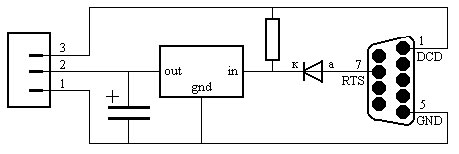
\includegraphics[width=8cm]{26_lirc_fig1}}
%\label{pic:fl1}
\caption{Схема инфракрасного приемника}
\end{figure}

\begin{figure}[ht]
\centering{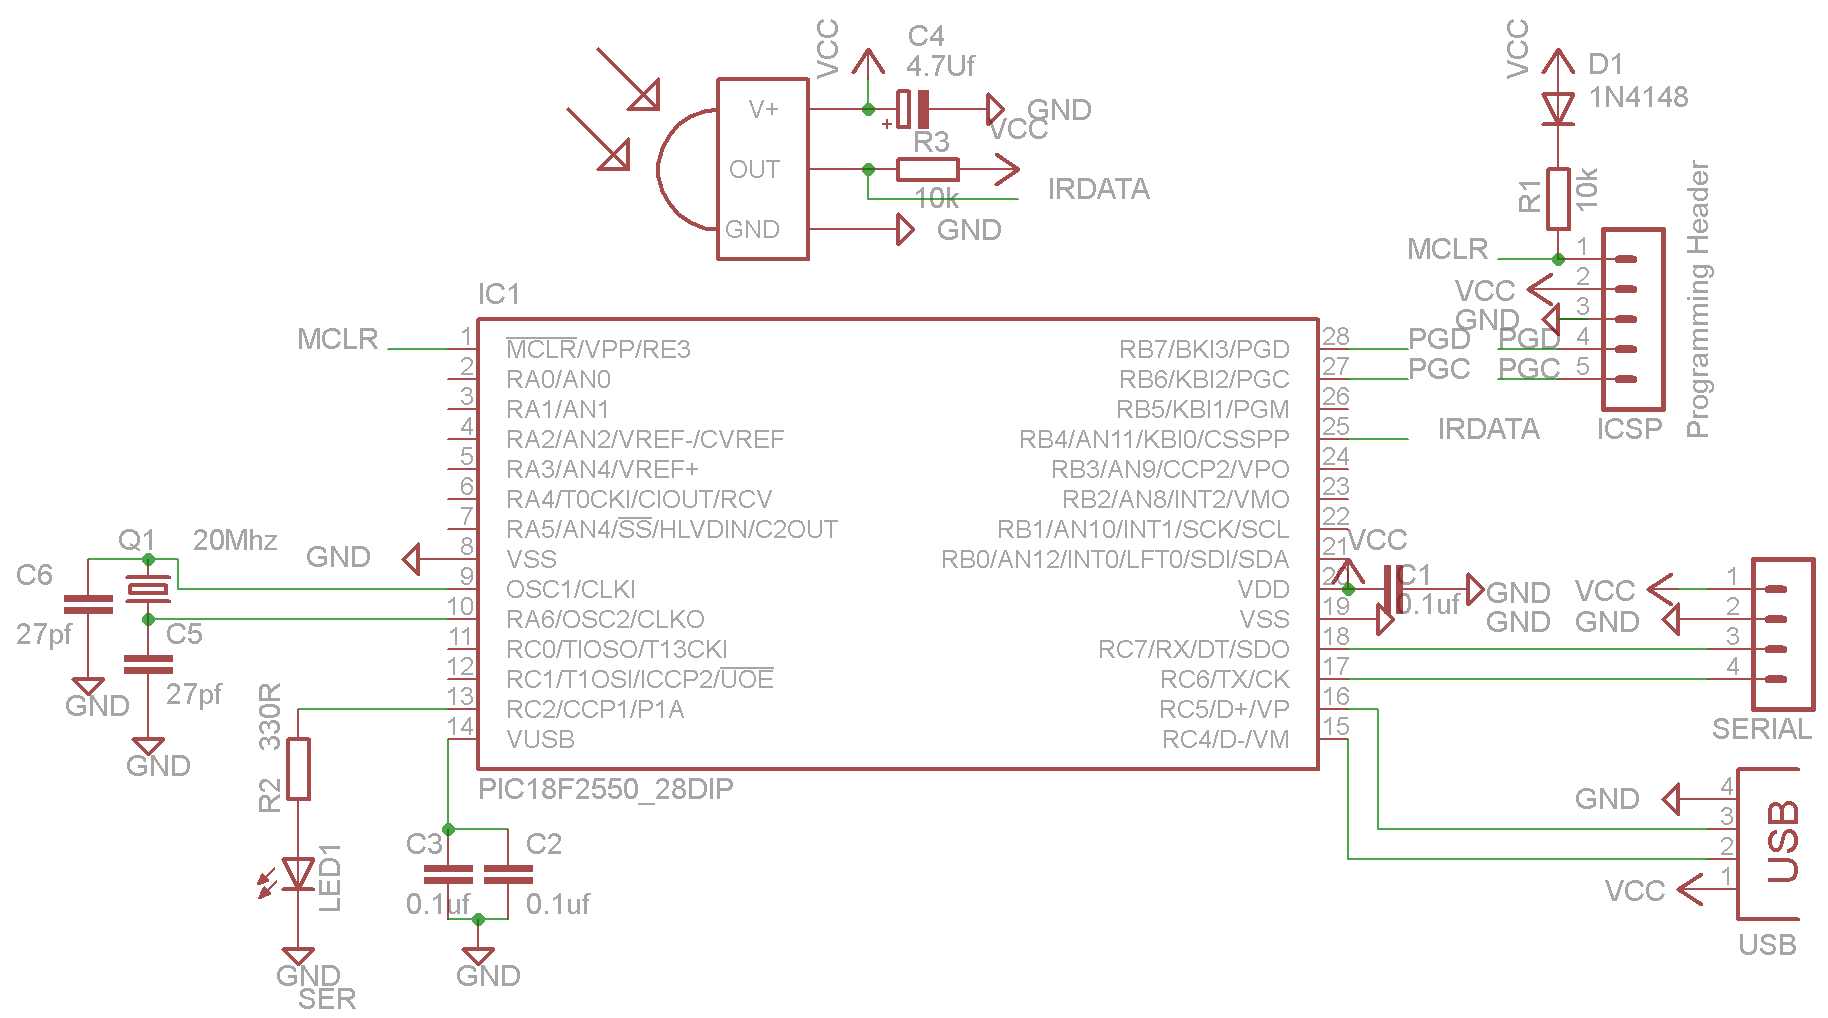
\includegraphics[width=8cm]{26_lirc_fig2}}
%\label{pic:fl1}
%\caption{Приложения по категориям}
\end{figure}

Такое решение является наиболее простым и доступным, однако, т.~к. COM-порт 
уже исчезающий вид интерфейса, более привлекательными выглядят
USB-приемники. Для его изготовления потребуется микроконтроллер.

Приемник базируется на микроконтроллере PIC18F2455, который может
работать с USB-портом и является меньшей и более дешевой версией
18F2550. Семейство 18F можно программировать при помощи универсального
PIC-программатора.

В состав пакета LIRC входят:
\begin{itemize}
	\item драйверы различных устройств (модули ядра)
	\item демон lircd, преобразующий ИК сигналы, полученные от драйвера, в стандартные сообщения, которые прикладные программы могут получить
через сокет 
\item демон lircmd, получающий сообщения от lircd и имитирующий мышь в X Windows
\item irexec "--- запуск программ по нажатию кнопки ДУ
\item irxevent "--- посылка X Windows сообщения по нажатию кнопки ДУ
\item irpty "--- псевдотерминал, запускающий программу и имитирущий нажатие клавиш клавиатуры
\end{itemize}
Кроме того, стоит упомянуть вспомогательные программы для отладки и настройки:
\begin{itemize}
	\item irrecord "--- утилита для записи сегналов пульта и создания lircd.conf
	\item irw "--- читает сообщения с сокета lircd и выдает на stdout; в качестве параметра можно указать имя сокета
	\item ircat "--- отладочная программа для конфигурационного файла ~/.lircrc; в качестве параметра указывается имя программы (точнее имя описывающей
её секции); по нажатию кнопки на пульте ДУ ircat выводит на stdout строку, привязанную к этой кнопке
\item mode2, smode2, xmode2 "--- осциллоскоп для инфракрасных сигналов
\item irsend "--- посылает команды на инфракрасные приемники (если позволяет оборудование)
\end{itemize}
В Linux существует множество приложений, направленных на централизованную работу с мультимедиа, например MythTV, Elisa,
XBMC. Однако, очевидно, что пульт может использоваться совместно с множеством других программных пакетов.

\end{document}



%\documentclass[10pt, a5paper]{article}
\usepackage{pdfpages}
\usepackage{parallel}
\usepackage[T2A]{fontenc}
\usepackage{ucs}
\usepackage[utf8x]{inputenc}
\usepackage[polish,english,russian]{babel}
\usepackage{hyperref}
\usepackage{rotating}
\usepackage[inner=2cm,top=1.8cm,outer=2cm,bottom=2.3cm,nohead]{geometry}
\usepackage{listings}
\usepackage{graphicx}
\usepackage{wrapfig}
\usepackage{longtable}
\usepackage{indentfirst}
\usepackage{array}
\newcolumntype{P}[1]{>{\raggedright\arraybackslash}p{#1}}
\frenchspacing
\usepackage{fixltx2e} %text sub- and superscripts
\usepackage{icomma} % коскі ў матэматычным рэжыме
\PreloadUnicodePage{4}

\newcommand{\longpage}{\enlargethispage{\baselineskip}}
\newcommand{\shortpage}{\enlargethispage{-\baselineskip}}

\def\switchlang#1{\expandafter\csname switchlang#1\endcsname}
\def\switchlangbe{
\let\saverefname=\refname%
\def\refname{Літаратура}%
\def\figurename{Іл.}%
}
\def\switchlangen{
\let\saverefname=\refname%
\def\refname{References}%
\def\figurename{Fig.}%
}
\def\switchlangru{
\let\saverefname=\refname%
\let\savefigurename=\figurename%
\def\refname{Литература}%
\def\figurename{Рис.}%
}

\hyphenation{admi-ni-stra-tive}
\hyphenation{ex-pe-ri-ence}
\hyphenation{fle-xi-bi-li-ty}
\hyphenation{Py-thon}
\hyphenation{ma-the-ma-ti-cal}
\hyphenation{re-ported}
\hyphenation{imp-le-menta-tions}
\hyphenation{pro-vides}
\hyphenation{en-gi-neering}
\hyphenation{com-pa-ti-bi-li-ty}
\hyphenation{im-pos-sible}
\hyphenation{desk-top}
\hyphenation{elec-tro-nic}
\hyphenation{com-pa-ny}
\hyphenation{de-ve-lop-ment}
\hyphenation{de-ve-loping}
\hyphenation{de-ve-lop}
\hyphenation{da-ta-ba-se}
\hyphenation{plat-forms}
\hyphenation{or-ga-ni-za-tion}
\hyphenation{pro-gramming}
\hyphenation{in-stru-ments}
\hyphenation{Li-nux}
\hyphenation{sour-ce}
\hyphenation{en-vi-ron-ment}
\hyphenation{Te-le-pathy}
\hyphenation{Li-nux-ov-ka}
\hyphenation{Open-BSD}
\hyphenation{Free-BSD}
\hyphenation{men-ti-on-ed}
\hyphenation{app-li-ca-tion}

\def\progref!#1!{\texttt{#1}}
\renewcommand{\arraystretch}{2} %Іначай формулы ў матрыцы зліпаюцца з лініямі
\usepackage{array}

\def\interview #1 (#2), #3, #4, #5\par{

\section[#1, #3, #4]{#1 -- #3, #4}
\def\qname{LVEE}
\def\aname{#1}
\def\q ##1\par{{\noindent \bf \qname: ##1 }\par}
\def\a{{\noindent \bf \aname: } \def\qname{L}\def\aname{#2}}
}

\def\interview* #1 (#2), #3, #4, #5\par{

\section*{#1\\{\small\rm #3, #4. #5}}

\def\qname{LVEE}
\def\aname{#1}
\def\q ##1\par{{\noindent \bf \qname: ##1 }\par}
\def\a{{\noindent \bf \aname: } \def\qname{L}\def\aname{#2}}
}

\begin{document}
\title{GRID-технологии в исследованиях дымовой плазмы}
\author{Сподарец Д.В., Драган Г.С.\footnote{Одесса, Украина, Одесский национальный университет имени И.И.Мечникова, \url{m31@root-ua.com}}}
\date{}
\maketitle
\begin{abstract}
The paper describes the use of GRID systems and computer clusters for smoky plasma research. Offers insight into the experience of expanding the functionality of TERM software and hardware complex for GRID systems.
\end{abstract}
В экспериментах все чаще используют  вычислительные кластеры и GRID-системы. Связано это с тем, что количество информации, полученное в следствии проведения эксперимента с использованием современного измерительного оборудования, достаточно велико. Немаловажным фактом, который играет роль при выборе супперкомпьютеров для автоматизации исследований и обработки результатов, является уменьшение ошибки измерений, а также возможность использовать новые технологии диагностики, например, позволяющие наблюдать процессы в реальном времени.

Основной объект наших исследований --- дымовая плазма. Она является разновидностью низкотемпературной термической плазмы с конденсированной дисперсной фазой, образуется в продуктах сгорания топлива и состоит из газовой фазы с легкоионизируемой примесью атомов щелочного металла и конденсированной в виде частиц оксидов металлов и сажи \cite{spod1}.

Для проведения диагностики таких параметров дымовой плазмы, как температура газовой и конденсированной фаз, концентрации электронов и атомов, нами был разработан аппаратно"=программный комплекс TERM \cite{spod2}. В его основе лежат оптические методы диагностики плазмы, а программная часть построена на свободном программном обеспечении. Среди новых возможностей комплекса, которые уже реализованы или находятся на стадии реализации, можно отметить дополнение его собственным вычислительным кластером, адаптация для работы в GRID-системах, разработка механизмов проведения виртуальных экспериментов \cite{spod3}.

Комплекс TERM работает следующим образом:
\begin{enumerate}
	\item Экспериментально определяется температура газовой и конденсированной фаз, а также концентрация электронов и атомов в плазме.
	\item На основе теории дымовой плазмы и измеренных экспериментально параметров проводится расчёт заряда частиц, а также определяется функция распределения частиц по заряду.
	\item Полученные данные зарядов используются для определения пространственного концентрационного неравновесия и сил \linebreak диффузионно-дрейфового давления свободных носителей заряда на частицы. Основой для данных расчётов служит теория обобщённого потенциала.
	\item Значения сил диффузионно-дрейфового давления учитываются при  расчёте парного взаимодействия частиц, а также в уравнениях молекулярной динамики для дымовой плазмы.
	\item Результатом работы комплекса является моделирование 3D структур заряженных конденсированных частичек в плазме. Этот этап проводится с использованием GRID Украины.
\end{enumerate}
Базовой ОС комплекса является ALT Linux. Для захвата и обработки видеопотоков применяется библиотека компьютерного зрения OpenCV. В качестве инструментария, при проведении расчётов, задействованы Octave и Mathematica. Разработан ряд собственных специфических алгоритмов, например, для проведения анализа спектров излучения плазмы. 

При совмещении реального физического эксперимента и виртуального моделирования на базе GRID Украины, стало возможным более глубокое изучение влияния объёмных и поверхностных процессов, происходящих в области пространственного заряда конденсированной частицы, на кинетику и динамику дымовой плазмы.
\begin{thebibliography}{9}
	\bibitem{spod1}Dragan G.S., Malgota A.A. et al. // Proc. Sc. and Tech. Meet., Alma-Ata, USSR, October 25-31, 1982. – Inst. High Temp., Acad. Sci. of the USSR, 1984. – P. 191 – 192. 
	\bibitem{spod2} http://term.m31.org.ua
	\bibitem{spod3} Spodarets D.V., Dragan G.S. Method of Experimental Research of Long-Range Interactions in Smoky Plasmas // Book of Abstr. of the ICPDP 2011, Garmasch-Partenkirchen. Germany.: 2011. P. 74. 
\end{thebibliography}
\end{document}



%\documentclass[10pt, a5paper]{article}
\usepackage{pdfpages}
\usepackage{parallel}
\usepackage[T2A]{fontenc}
\usepackage{ucs}
\usepackage[utf8x]{inputenc}
\usepackage[polish,english,russian]{babel}
\usepackage{hyperref}
\usepackage{rotating}
\usepackage[inner=2cm,top=1.8cm,outer=2cm,bottom=2.3cm,nohead]{geometry}
\usepackage{listings}
\usepackage{graphicx}
\usepackage{wrapfig}
\usepackage{longtable}
\usepackage{indentfirst}
\usepackage{array}
\newcolumntype{P}[1]{>{\raggedright\arraybackslash}p{#1}}
\frenchspacing
\usepackage{fixltx2e} %text sub- and superscripts
\usepackage{icomma} % коскі ў матэматычным рэжыме
\PreloadUnicodePage{4}

\newcommand{\longpage}{\enlargethispage{\baselineskip}}
\newcommand{\shortpage}{\enlargethispage{-\baselineskip}}

\def\switchlang#1{\expandafter\csname switchlang#1\endcsname}
\def\switchlangbe{
\let\saverefname=\refname%
\def\refname{Літаратура}%
\def\figurename{Іл.}%
}
\def\switchlangen{
\let\saverefname=\refname%
\def\refname{References}%
\def\figurename{Fig.}%
}
\def\switchlangru{
\let\saverefname=\refname%
\let\savefigurename=\figurename%
\def\refname{Литература}%
\def\figurename{Рис.}%
}

\hyphenation{admi-ni-stra-tive}
\hyphenation{ex-pe-ri-ence}
\hyphenation{fle-xi-bi-li-ty}
\hyphenation{Py-thon}
\hyphenation{ma-the-ma-ti-cal}
\hyphenation{re-ported}
\hyphenation{imp-le-menta-tions}
\hyphenation{pro-vides}
\hyphenation{en-gi-neering}
\hyphenation{com-pa-ti-bi-li-ty}
\hyphenation{im-pos-sible}
\hyphenation{desk-top}
\hyphenation{elec-tro-nic}
\hyphenation{com-pa-ny}
\hyphenation{de-ve-lop-ment}
\hyphenation{de-ve-loping}
\hyphenation{de-ve-lop}
\hyphenation{da-ta-ba-se}
\hyphenation{plat-forms}
\hyphenation{or-ga-ni-za-tion}
\hyphenation{pro-gramming}
\hyphenation{in-stru-ments}
\hyphenation{Li-nux}
\hyphenation{sour-ce}
\hyphenation{en-vi-ron-ment}
\hyphenation{Te-le-pathy}
\hyphenation{Li-nux-ov-ka}
\hyphenation{Open-BSD}
\hyphenation{Free-BSD}
\hyphenation{men-ti-on-ed}
\hyphenation{app-li-ca-tion}

\def\progref!#1!{\texttt{#1}}
\renewcommand{\arraystretch}{2} %Іначай формулы ў матрыцы зліпаюцца з лініямі
\usepackage{array}

\def\interview #1 (#2), #3, #4, #5\par{

\section[#1, #3, #4]{#1 -- #3, #4}
\def\qname{LVEE}
\def\aname{#1}
\def\q ##1\par{{\noindent \bf \qname: ##1 }\par}
\def\a{{\noindent \bf \aname: } \def\qname{L}\def\aname{#2}}
}

\def\interview* #1 (#2), #3, #4, #5\par{

\section*{#1\\{\small\rm #3, #4. #5}}

\def\qname{LVEE}
\def\aname{#1}
\def\q ##1\par{{\noindent \bf \qname: ##1 }\par}
\def\a{{\noindent \bf \aname: } \def\qname{L}\def\aname{#2}}
}

\begin{document}
\title{Свободное производство информации в постиндустриальном обществе}
\author{Елена Иванова\footnote{Москва, Россия, \url{http://coofeed.com}}, Дмитрий Костюк\footnote{Брест, Беларусь, \url{dmitriykostiuk@gmail.com}}}
\date{}
\maketitle
\begin{abstract}
The concept of postindustrial society is discussed in relation to free / open source software community-driven production. Its better correlation with Bell principles than classic information-as-a-good approach is shown. 
\end{abstract}

Концепция постиндустриализма в качестве следующей стадии социального развития приобрела широкую известность в 1970-х годах, когда Д. Беллом были сформулированы следующие положения \cite{ivanova1}, лежащие в его основе: главенствующая роль знаний в обществе (1), главенствующая роль производства не товаров, но услуг (2), университет как очаг производства новых знаний и инноваций (3). Исходно реализацию перечисленных принципов затрудняла дороговизна и малая эффективность коммуникации между специалистами. Ставшая популярной в 90-х концепция информационного общества \cite{ivanova2} включила в себя построение глобального информационного пространства с использованием новых компьютерных технологий, и таким образом в значительной степени снизила коммуникационный барьер за счет на порядок более эффективного удаленного взаимодействия.

Популярное толкование положения о информации и знаниях, как главном продукте производства, рассматривает поточное производство информации как товара в рамках сервисной (т. е. ориентированной на рынок услуг) экономики. В определенном смысле первый и третий из сформулированных Беллом признаков постиндустриального общества рассматриваются в качестве сателлитов положения о примате производства услуг. 

Производство информации более прибыльно в сравнении с материальным производством, так как достаточно изготовить первоначальный образец, а затраты на копирование несущественны. Но эти же свойства информации делают ее неудобным товаром с точки зрения традиционных экономических отношений. Когда под предоставлением услуг понимается торговля информацией или сдача информации в аренду, приходится изобретать искусственные ограничительные механизмы. Необходима развитая юридическая защита прав интеллектуальной собственности. Права на информацию, которые подлежат юридической защите, должны носить монопольный характер (это является не только необходимым условием для превращения информации в товар, но и позволяет извлекать монопольную прибыль, увеличивая рентабельность постиндустриальной экономики). Необходимо огромное количество потребителей, которые готовы платить за информацию, предоставляемую в данной ограниченной форме.

Однако возрастание числа людей, занятых информационными технологиями, коммуникациями и производством информационных продуктов и услуг "--- людей, основным «средством производства» которых является не оборудование работодателя, а их собственная квалификация \cite{ivanova2} "--- вносит в данный подход коррективы. В результате, существенная часть членов общества оказывается неудовлетворенной накладываемыми на информационный продукт искусственными ограничениями, делающими его использование менее удобным и осознает, что сверхприбыли поставщиков информационного продукта противоречат интересам их, как потребителей. Такая группа имеет средства производства для коллективного воссоздания аналога и сетевую инфраструктуру, позволяющую добиться предсказанной апологетами постиндустриализма быстрой самоорганизации творческих коллективов для решения конкретных задач, а ее представители готовы воспринимать в качестве опосредованного источника прибыли дополнительные факторы, такие как рост личного профессионализма и профессиональную репутацию.

Наиболее ярко на сегодняшний день данное явление проявляется в сфере свободного программного обеспечения. Группы специалистов, неудовлетворенные ситуацией на рынке, объединяются, выделяя часть своего свободного времени (являющегося в постиндустриальном обществе оцениваемым ресурсом) для создания равноценного программного продукта, свободного от искусственных ограничений, связанных с интеллектуальной монополией \cite{ivanova3} какого-либо производителя. В качестве страховки интересов потребителей такой продукт часто оснащается собственными лицензионными ограничениями, направленными против его возможной монополизации.
В рамках сформулированной концепции информационного общества данное явление можно рассматривать как массовое коллективное инвестирование, базирующееся на совладении материальными и нематериальными активами (crowd funding). Характерно также, что первоначальными источниками появления свободных программ являлись университеты, в полном соответствии с одним из сформулированных Беллом положений.

Модели бизнеса, построенные вокруг таких продуктов, хорошо укладываются в постиндустриальную модель, предоставляя коммерческие услуги по сопровождению и/или доработке продукта, а также доступ к продукту (консолидированному и обслуживаемому централизованно на мощных вычислительных станциях) в рамках облачных вычислений и технологии Software-As-Service (приложение как услуга).

Явление коллективного производства свободно распространяемых информационных продуктов претерпевает некоторые эволюционные изменения, связанные с большей доступностью для потребителя и проникновением в смежные области, примером чему служат коллективное создание высококачественного энциклопедического контента википедии и родственных проектов, а также активизация на рынке средств мобильной связи. В частности, идеи объединения функциональности сотового телефона и карманного персонального компьютера появились практически сразу после появления первых карманных персональных компьютеров в начале 90-х. Наличие полнофункциональной операционной системы делает смартфоны и коммуникаторы более привлекательными в глазах большинства пользователей. Современные телефоны прекрасно справляются со многими задачами, выходящими за рамки телефонных: работа с электронной почтой, просмотр текстовых документов и электронных таблиц, работа с планировщиком задач и многими другими. Однако резкий рост популярности смартфонов произошел одновременно с развитием инфраструктуры открытой операционной системы Android \cite{ivanova4}.
Аналогичным по своей сути направлением эволюции в компьютерных технологиях является децентрализация, примером которой могут служить файловый обмен (торенты), электронные системы платежей, такие как BitCoin \cite{ivanova5}, распределенные социальные сети.

\newpage\begin{thebibliography}{9}
	\bibitem{ivanova1} Д. Белл. Грядущее постиндустриальное общество. М., Академия, 1999.
	\bibitem{ivanova2} Постиндустриальное общество. \url{http://ru.wikipedia.org}  
	\bibitem{ivanova3} Л. Лессиг. Свободная культура. \url{http://www.gumer.info/bibliotek_Buks/Culture/lessig/index.php}
	\bibitem{ivanova4} Source: Gartner (May 2011) \url{http://www.gartner.com/it/page.jsp?id=1689814}
	\bibitem{ivanova5} BitCoin --- анархическая пиринговая криптовалюта. \url{http://blogerator.ru/page/bitcoin}
\end{thebibliography}
\end{document}



%\documentclass[10pt, a5paper]{article}
\usepackage{pdfpages}
\usepackage{parallel}
\usepackage[T2A]{fontenc}
\usepackage{ucs}
\usepackage[utf8x]{inputenc}
\usepackage[polish,english,russian]{babel}
\usepackage{hyperref}
\usepackage{rotating}
\usepackage[inner=2cm,top=1.8cm,outer=2cm,bottom=2.3cm,nohead]{geometry}
\usepackage{listings}
\usepackage{graphicx}
\usepackage{wrapfig}
\usepackage{longtable}
\usepackage{indentfirst}
\usepackage{array}
\newcolumntype{P}[1]{>{\raggedright\arraybackslash}p{#1}}
\frenchspacing
\usepackage{fixltx2e} %text sub- and superscripts
\usepackage{icomma} % коскі ў матэматычным рэжыме
\PreloadUnicodePage{4}

\newcommand{\longpage}{\enlargethispage{\baselineskip}}
\newcommand{\shortpage}{\enlargethispage{-\baselineskip}}

\def\switchlang#1{\expandafter\csname switchlang#1\endcsname}
\def\switchlangbe{
\let\saverefname=\refname%
\def\refname{Літаратура}%
\def\figurename{Іл.}%
}
\def\switchlangen{
\let\saverefname=\refname%
\def\refname{References}%
\def\figurename{Fig.}%
}
\def\switchlangru{
\let\saverefname=\refname%
\let\savefigurename=\figurename%
\def\refname{Литература}%
\def\figurename{Рис.}%
}

\hyphenation{admi-ni-stra-tive}
\hyphenation{ex-pe-ri-ence}
\hyphenation{fle-xi-bi-li-ty}
\hyphenation{Py-thon}
\hyphenation{ma-the-ma-ti-cal}
\hyphenation{re-ported}
\hyphenation{imp-le-menta-tions}
\hyphenation{pro-vides}
\hyphenation{en-gi-neering}
\hyphenation{com-pa-ti-bi-li-ty}
\hyphenation{im-pos-sible}
\hyphenation{desk-top}
\hyphenation{elec-tro-nic}
\hyphenation{com-pa-ny}
\hyphenation{de-ve-lop-ment}
\hyphenation{de-ve-loping}
\hyphenation{de-ve-lop}
\hyphenation{da-ta-ba-se}
\hyphenation{plat-forms}
\hyphenation{or-ga-ni-za-tion}
\hyphenation{pro-gramming}
\hyphenation{in-stru-ments}
\hyphenation{Li-nux}
\hyphenation{sour-ce}
\hyphenation{en-vi-ron-ment}
\hyphenation{Te-le-pathy}
\hyphenation{Li-nux-ov-ka}
\hyphenation{Open-BSD}
\hyphenation{Free-BSD}
\hyphenation{men-ti-on-ed}
\hyphenation{app-li-ca-tion}

\def\progref!#1!{\texttt{#1}}
\renewcommand{\arraystretch}{2} %Іначай формулы ў матрыцы зліпаюцца з лініямі
\usepackage{array}

\def\interview #1 (#2), #3, #4, #5\par{

\section[#1, #3, #4]{#1 -- #3, #4}
\def\qname{LVEE}
\def\aname{#1}
\def\q ##1\par{{\noindent \bf \qname: ##1 }\par}
\def\a{{\noindent \bf \aname: } \def\qname{L}\def\aname{#2}}
}

\def\interview* #1 (#2), #3, #4, #5\par{

\section*{#1\\{\small\rm #3, #4. #5}}

\def\qname{LVEE}
\def\aname{#1}
\def\q ##1\par{{\noindent \bf \qname: ##1 }\par}
\def\a{{\noindent \bf \aname: } \def\qname{L}\def\aname{#2}}
}

\begin{document}
\title{Протокол IF-MAP}
\author{Олег Орел\footnote{Минск, Беларусь, EPAM Systems, \url{Aleh_Arol@epam.com}}}
\date{}
\maketitle
\begin{abstract}
The Interface for Metadata Access Points (IF-MAP) is an open standard client/server protocol developed as one of the core protocols of the Trusted Network Connect (TNC) open architec\-ture. IF-MAP provides a common interface between the database server acting as a clearinghouse for information about security events and objects, and other elements of the TNC architecture.
\end{abstract}

TNC (Trusted Network Connect) "--- архитектура, описывающая возможную реализацию подхода к сетевой компьютерной безопасности, унифицирующего решения по обеспечению безопасности на конечных узлах (такие как антивирусное ПО, системы обнаружения вторжений и т.~д.), пользовательскую аутентификацию, элементы обеспечения безопасности. Компьютер, подключившийся в сеть, получает уровень доступа к ресурсам по результатам анализа таких его параметров, как уровень защищенности от вредоносных программ, конфигурации, роли пользователя, обновлений ОС. По любому параметру доступ может быть разграничен: например, пользователь, чей компьютер не обладает свежими антивирусными базами, не будет допущен в Интернет. IF"=MAP "--- открытый стандарт, описывающий клиент"=серверный протокол обмена данных между элементами (MAP) в TNC"=архитектуре.
IF-MAP сервер "--- это централизованное хранилище метаданных (например, о состоянии узлов сети, пользователях и т.~д.), предоставляющее механизмы для публикации данных, поиска и подписок всем заинтересованным MAP"=клиентам. Модель данных, предусмотренная для IF-MAP сервиса, представляет собой граф, вершины которого "--- идентификаторы (device, ip-address, mac-address, access-request, \ldots), а ребра "--- метаданные. Например, метаданные типа ip-mac, которые публикует MAP"=клиент, работающий совместно с DHCP сервером, соединяют идентификаторы типа ip"=address и mac"=address (DHCP lease) и содержат дополнительную информацию (время действия адреса). MAP"=клиентам доступен поиск на этом графе, а система подписок на изменения позволяет выполнять отложенный поиск.


\end{document}



\documentclass[10pt, a5paper]{article}
\usepackage{pdfpages}
\usepackage{parallel}
\usepackage[T2A]{fontenc}
\usepackage{ucs}
\usepackage[utf8x]{inputenc}
\usepackage[polish,english,russian]{babel}
\usepackage{hyperref}
\usepackage{rotating}
\usepackage[inner=2cm,top=1.8cm,outer=2cm,bottom=2.3cm,nohead]{geometry}
\usepackage{listings}
\usepackage{graphicx}
\usepackage{wrapfig}
\usepackage{longtable}
\usepackage{indentfirst}
\usepackage{array}
\newcolumntype{P}[1]{>{\raggedright\arraybackslash}p{#1}}
\frenchspacing
\usepackage{fixltx2e} %text sub- and superscripts
\usepackage{icomma} % коскі ў матэматычным рэжыме
\PreloadUnicodePage{4}

\newcommand{\longpage}{\enlargethispage{\baselineskip}}
\newcommand{\shortpage}{\enlargethispage{-\baselineskip}}

\def\switchlang#1{\expandafter\csname switchlang#1\endcsname}
\def\switchlangbe{
\let\saverefname=\refname%
\def\refname{Літаратура}%
\def\figurename{Іл.}%
}
\def\switchlangen{
\let\saverefname=\refname%
\def\refname{References}%
\def\figurename{Fig.}%
}
\def\switchlangru{
\let\saverefname=\refname%
\let\savefigurename=\figurename%
\def\refname{Литература}%
\def\figurename{Рис.}%
}

\hyphenation{admi-ni-stra-tive}
\hyphenation{ex-pe-ri-ence}
\hyphenation{fle-xi-bi-li-ty}
\hyphenation{Py-thon}
\hyphenation{ma-the-ma-ti-cal}
\hyphenation{re-ported}
\hyphenation{imp-le-menta-tions}
\hyphenation{pro-vides}
\hyphenation{en-gi-neering}
\hyphenation{com-pa-ti-bi-li-ty}
\hyphenation{im-pos-sible}
\hyphenation{desk-top}
\hyphenation{elec-tro-nic}
\hyphenation{com-pa-ny}
\hyphenation{de-ve-lop-ment}
\hyphenation{de-ve-loping}
\hyphenation{de-ve-lop}
\hyphenation{da-ta-ba-se}
\hyphenation{plat-forms}
\hyphenation{or-ga-ni-za-tion}
\hyphenation{pro-gramming}
\hyphenation{in-stru-ments}
\hyphenation{Li-nux}
\hyphenation{sour-ce}
\hyphenation{en-vi-ron-ment}
\hyphenation{Te-le-pathy}
\hyphenation{Li-nux-ov-ka}
\hyphenation{Open-BSD}
\hyphenation{Free-BSD}
\hyphenation{men-ti-on-ed}
\hyphenation{app-li-ca-tion}

\def\progref!#1!{\texttt{#1}}
\renewcommand{\arraystretch}{2} %Іначай формулы ў матрыцы зліпаюцца з лініямі
\usepackage{array}

\def\interview #1 (#2), #3, #4, #5\par{

\section[#1, #3, #4]{#1 -- #3, #4}
\def\qname{LVEE}
\def\aname{#1}
\def\q ##1\par{{\noindent \bf \qname: ##1 }\par}
\def\a{{\noindent \bf \aname: } \def\qname{L}\def\aname{#2}}
}

\def\interview* #1 (#2), #3, #4, #5\par{

\section*{#1\\{\small\rm #3, #4. #5}}

\def\qname{LVEE}
\def\aname{#1}
\def\q ##1\par{{\noindent \bf \qname: ##1 }\par}
\def\a{{\noindent \bf \aname: } \def\qname{L}\def\aname{#2}}
}

\begin{document}
\title{Голос спонсора: SaM Solutions}
%\author{}
\date{}
\maketitle

Компания SaM Solutions выступает в роли системо-образующего спонсора конференции Linux Vacation Eastern Europe с момента рождения LVEE в 2005 году и на протяжении всех лет её проведения. 

Сложившаяся корпоративная практика не случайна. Продукты и решения, задействующие Linux и другие Free/Open Source Software проекты, составляют заметную часть пакета разработок SaM Solutions. Кадровая политика компании направлена на поощрение профессионального развития своих сотрудников, организацию их эффективного отдыха и привлечение хорошо мотивированных кандидатов к работе на компанию. Формат конференции LVEE успешно позволяет решать все три задачи. 

Одним из подразделений компании является отдел Linux и \linebreak Embbeded. Специалисты компании на протяжении десятилетий работают с СПО. Компанией реализован ряд проектов по адаптации ОС GNU/Linux для работы в различных устройствах, построенных на таких платформах как ARM, PowerPC, x86, MIPS. В последние годы "--- на ведущие позиции выходит разработка управляющего ПО для серверов Enterprise-класса, от низкоуровнего BMC Firmware на основе Linux до высокоуровневых систем контроля виртуализации и графических интерфейсов управления, от прошивок устройств хранения данных до BSP интегрированных плат для разработчика. Надёжность, качество и широкая функциональность множества свободных проектов позволяет строить нам системы любого уровня и сложности, опираясь на высококачественные готовые компоненты.

В рамках направления Linux и Embedded успешно выполнены проекты для таких знаковых заказчиков, как  Novell/SUSE, Fujitsu Technology Solutions  и осуществляется партнёрство с компаниями IBM и Oracle/Sun в области Open Source решений.

Мы разрабатываем, модифицируем и адаптируем различное свободное программное обеспечение для наших заказчиков, но не забываем и о своих нуждах "--- наши сотрудники используют в своей работе существующие програмные продукты и вносят вклад в их развитие. Часть внутренней инфраструктуры, а именно интранет-сеть компании, тестовые стенды отдела контроля качества, рабочие места сотрудников профильных подразделений "--- также работает под управлением СПО (серверные и десктопные платформы GNU/Linux и FreeBSD). 

В минувшем году, в рамках реорганизации, был разработан долгосрочный план развития направления Linux и Embedded в SaM Solutions. В нём впервые были кодифицированы уже имеющиеся внутренние неофициальные практики по взаимодействию с commu"=nity-based проектами. В частности разработаны меры и правила по
\begin{itemize}
  \item возврата изменений в родительские проекты (upstreaming);
  \item вхождения в состав постоянных разработчиков активно используемых нами FOSS-компонентов;
  \item публикации сообщений об ошибках (bug reporting);
  \item участия и помощи в организации community events;
  \item стимуляции докладов и участия в технических конференциях.
\end{itemize}
И план немедленно начал претворяться в жизнь.

Силами отдела организовано внутреннее обучение сотрудников на регулярной
основе. Был прочтен и опубликован курс по TDD. По согласованию с автором
опубликован курс Debian/Ubuntu Packaging (видео, презентация и исходные
тексты презентации в \LaTeX).  Были организованы и проведены курсы по
обучению QA специалистов для направления Embeded Linux. Проведено
практическое занятие по основам виртуализации и эмуляции, организована
лекция по вопросу профилирования и оптимизации Ruby-кода, лекция о
High-availability кластерах и направлении развития технологии. Кроме того,
проводился семинар по Video4Linux2. Для создания и обучения кадрового
резерва на ближайшее будущее запланированы постоянно действующие внутренние
проекты в области Embedded Linux, результаты которых также запланированы к
публикации.

Визиты представительных делегаций на Embedded World 2012 и Linux Con Europe/Embedded LinuxCon Europe 2011 обогатили нас новыми идеями, куда можно
двигаться дальше и что сейчас актуально. А выступления на Software
Engineering Forum for Students, круглом столе по СПО в рамках TIBO-2012
и LVEE Winter 2012 позволили поделиться опытом с
заинтересованными сторонами.

В апреле состоялась Ганноверская промышленная ярмарка \linebreak (Hannover Messe
2013). Компания SaM Solutions была представлена отдельным стендом, на
котором демонстрировались наработки в области встроенного и системного ПО
на базе OS Linux. Идея «умного» дома вызвала неподдельный интерес у
посетителей стенда.

При поддержке SaM Solutions, с декабря 2011 года возобновились регулярные встречи Minsk Linux Users Groups, под названием <<Линуксовка в SaM Solutions>>. Техническое оснащение линуксовок и открытый формат встреч позволил им практически мгновенно стать заметным дискуссионным клубом по широкому спектру вопросов, прямо или косвенно связанных с СПО. Свободная картография (OpenStreetMap), технологии виртуализации, минский \linebreak hackerspace, Linux Mobile, бойкот Голливудской продукции, systemd, загрузчик u-boot, белорусская локализация GNOME --- это только часть тем, поднятых за последние линуксовки.

Быстрые и положительные изменения, как внутри компании SaM Solutions, так и в экосфере СПО (и Linux в частности) наполняют нас уверенностью, что направление движения выбрано верно.

\begin{figure}[h!]
\centering
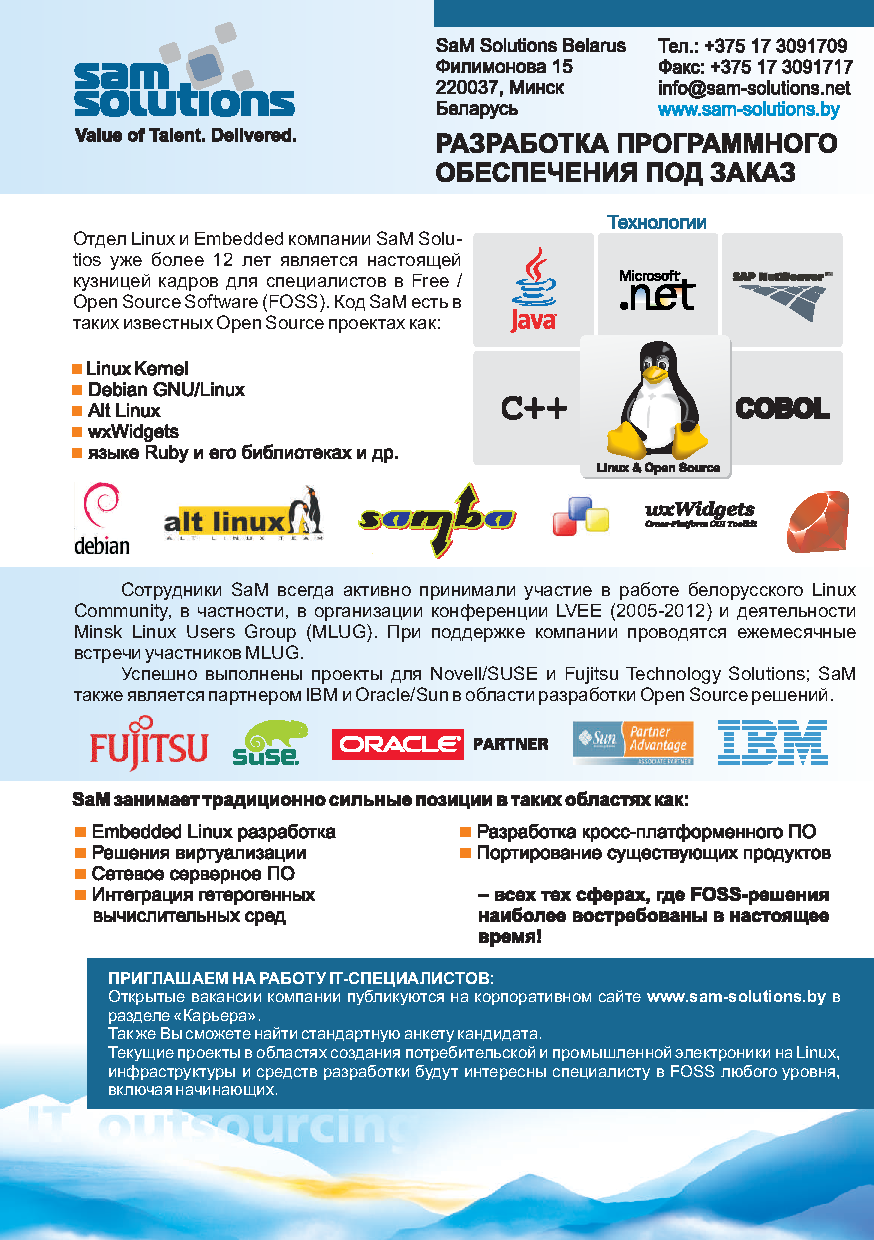
\includegraphics[height=11.8cm]{48_spons_sams.pdf}
\end{figure}
\end{document}



\documentclass[10pt, a5paper]{article}
\usepackage{pdfpages}
\usepackage{parallel}
\usepackage[T2A]{fontenc}
\usepackage{ucs}
\usepackage[utf8x]{inputenc}
\usepackage[polish,english,russian]{babel}
\usepackage{hyperref}
\usepackage{rotating}
\usepackage[inner=2cm,top=1.8cm,outer=2cm,bottom=2.3cm,nohead]{geometry}
\usepackage{listings}
\usepackage{graphicx}
\usepackage{wrapfig}
\usepackage{longtable}
\usepackage{indentfirst}
\usepackage{array}
\newcolumntype{P}[1]{>{\raggedright\arraybackslash}p{#1}}
\frenchspacing
\usepackage{fixltx2e} %text sub- and superscripts
\usepackage{icomma} % коскі ў матэматычным рэжыме
\PreloadUnicodePage{4}

\newcommand{\longpage}{\enlargethispage{\baselineskip}}
\newcommand{\shortpage}{\enlargethispage{-\baselineskip}}

\def\switchlang#1{\expandafter\csname switchlang#1\endcsname}
\def\switchlangbe{
\let\saverefname=\refname%
\def\refname{Літаратура}%
\def\figurename{Іл.}%
}
\def\switchlangen{
\let\saverefname=\refname%
\def\refname{References}%
\def\figurename{Fig.}%
}
\def\switchlangru{
\let\saverefname=\refname%
\let\savefigurename=\figurename%
\def\refname{Литература}%
\def\figurename{Рис.}%
}

\hyphenation{admi-ni-stra-tive}
\hyphenation{ex-pe-ri-ence}
\hyphenation{fle-xi-bi-li-ty}
\hyphenation{Py-thon}
\hyphenation{ma-the-ma-ti-cal}
\hyphenation{re-ported}
\hyphenation{imp-le-menta-tions}
\hyphenation{pro-vides}
\hyphenation{en-gi-neering}
\hyphenation{com-pa-ti-bi-li-ty}
\hyphenation{im-pos-sible}
\hyphenation{desk-top}
\hyphenation{elec-tro-nic}
\hyphenation{com-pa-ny}
\hyphenation{de-ve-lop-ment}
\hyphenation{de-ve-loping}
\hyphenation{de-ve-lop}
\hyphenation{da-ta-ba-se}
\hyphenation{plat-forms}
\hyphenation{or-ga-ni-za-tion}
\hyphenation{pro-gramming}
\hyphenation{in-stru-ments}
\hyphenation{Li-nux}
\hyphenation{sour-ce}
\hyphenation{en-vi-ron-ment}
\hyphenation{Te-le-pathy}
\hyphenation{Li-nux-ov-ka}
\hyphenation{Open-BSD}
\hyphenation{Free-BSD}
\hyphenation{men-ti-on-ed}
\hyphenation{app-li-ca-tion}

\def\progref!#1!{\texttt{#1}}
\renewcommand{\arraystretch}{2} %Іначай формулы ў матрыцы зліпаюцца з лініямі
\usepackage{array}

\def\interview #1 (#2), #3, #4, #5\par{

\section[#1, #3, #4]{#1 -- #3, #4}
\def\qname{LVEE}
\def\aname{#1}
\def\q ##1\par{{\noindent \bf \qname: ##1 }\par}
\def\a{{\noindent \bf \aname: } \def\qname{L}\def\aname{#2}}
}

\def\interview* #1 (#2), #3, #4, #5\par{

\section*{#1\\{\small\rm #3, #4. #5}}

\def\qname{LVEE}
\def\aname{#1}
\def\q ##1\par{{\noindent \bf \qname: ##1 }\par}
\def\a{{\noindent \bf \aname: } \def\qname{L}\def\aname{#2}}
}

\begin{document}
\title{Голос спонсора: EPAM Systems}
%\author{}
\date{}
\maketitle

Компания EPAM Systems не первый год является спонсором международной конференции разработчиков и пользователей свободного программного обеспечения LVEE (Linux Vacation / Eastern Europe). Этот год также не стал исключением. Пожалуй, LVEE является самым значимым событием для русскоязычных разработчиков и тестировщиков Open Source. Каждое лето здесь встречаются начинающие специалисты и «ветераны»"=разработчики из десятка стран для обмена опытом и общения на профессиональные темы. Наши специалисты также активно участвуют в данной конференции: в качестве докладчиков и организаторов/волонтёров. Это уникальная в своём роде конференция, и именно поэтому EPAM Systems очередной раз принимает участие в LVEE в качестве спонсора.


EPAM Systems "--- одна из крупнейших компаний"=поставщиков\linebreak услуг в области разработки программного обеспечения и решений на территории СНГ и Центральной и Восточной Европы. Созданная в 1993 году, сегодня она имеет представительства в 12 странах мира, в штате работают более 9 тыс. сотрудников, из которых более 3 тыс. "--- в Беларуси. Рост компании обеспечивается за счет собственных обучающих программ и передаче опыта от больших специалистов до начинающих разработчиков. Компания EPAM Systems выполняет проекты более чем в 30 странах мира. Основные направления деятельности: разработка, тестирование, сопровождение и поддержка заказного программного обеспечения и бизнес"=приложений, а также ИТ"=консалтинг с учетом отраслевой специфики бизнеса.

Наша компания участвует в проектах с такими крупными, хорошо известными заказчиками как Google, Novell, Infoblox, Parallels, 10Gen и др., так и с небольшими, в том числе и с начинающими свой путь в софтверном бизнесе.


К примеру, для Infoblox была реализована связка между WebUI с BIND и DHCP. Для этого был разработан комплекс решений под управлением Shell и Python скриптов, а также механизм позволяющий вносить правки в BIND и DHCP на языке C. Также был разработан развернутый функционал, автоматизирующий инсталляцию новых устройств и их эксплуатацию, что позволяет значительно упростить управление данными. Встроенный Web"=интерфейс позволяет разворачивать, управлять сервисами DNS, DNSSEC, DHCP, IPAM, устанавливать новые версии ПО, архивировать и восстанавливать из архивов необходимые данные, восстанавливать их после аварии, проводить мониторинг сети и создавать отчеты без необходимости обращения к командной строке.


Еще одним решением, реализованным для компании Infoblox, являлся программный продукт, позволяющий контролировать сетевые изменения, таким образом, облегчая идентификацию трудноуловимых проблем конфигурации и соответствие требованиям. Вместо того чтобы просто регистрировать изменения, система использует внесенную информацию для проверки, анализа и автоматической обработки сетевых изменений. Благодаря инновационной, квалифицированной, глубокой технике логического анализа, программа изолирует проблемы исправности и конфигурации до того, как они могут вызвать более серьезные сбои.


Разработанная для анализа сложных сетей система изучает сеть, собирает ключевую информацию, применяет встроенную технику логического анализа и создает оценку исправности сети и список проблем, требующих принятие мер для улучшения качества работы сети.


Правильное использование свободного ПО в разработках сокращает и расходы на покупку лицензионных программ, и трудозатраты при создании коммерческого ПО. Немалую роль для достижения превосходного результата играет привлечение к разработке опытных специалистов. LVEE способствует появлению таких специалистов, развитию их навыков и расширению кругозора. Хотелось бы пожелать участникам конференции интересных проектов и максимум пользы от участия в LVEE.


\end{document}



%\documentclass[10pt, a5paper]{article}
\usepackage{ucs}
\usepackage[utf8]{inputenc}
\usepackage[T2A]{fontenc}
\usepackage[english, russian]{babel}
\usepackage{hyperref}
\usepackage{geometry}
\usepackage{graphicx}
\frenchspacing
\begin{document}
\title{Голос спонсора: Ciklum}
%\author{}
\date{}
\maketitle
\begin{figure}[ht]
\centering{
\includegraphics[width=12cm]{51_spons_ciklum1}}
%\label{pic:fl1}
%\caption{Схема инфракрасного приемника}
\end{figure}

Ciklum is a Danish innovative IT outsourcing company specializing in nearshore software development. 
Established in 2002, Ciklum employs more than 1200+ IT specialists worldwide with more than 130+ current clients own development teams. Ciklum has pioneered a unique business model in Ukraine where employees have direct communication with the client and are equal to clients` home-based colleagues. In Ciklum we are working on the development of different kind of projects: from cross-platform end-user applications to multifunctional B2B scalable solutions.

What Ciklum offers to developers?
\begin{itemize}
\item Variety of knowledge sharing and training opportunities within Ciklum Knowledge Exchange community
\item A lot of various technical seminars
\item Unique working environment where you communicate and work directly with international businesses
\item Possibility to work in a big and successful company
\item Competitive salary
\item Career and professional growth 
\item Long-term employment with 20 working-days paid vacation and other social benefits 
\item State of the art, cool, centrally located offices with warm atmosphere which creates really good working conditions
\end{itemize}

Ciklum has four development offices in the four largest cities in Ukraine \& Belarus (Kyiv, Minsk, Kharkiv, Dnipropetrovsk, Donetsk) and two development offices in Pakistan (Lahore, Islamabad), as well as representative offices in Denmark, Sweden, United Kingdom, Switzerland, Germany and the Netherlands. 

Join Ciklum and «Cross the Borders» together with us!

\begin{figure}[hb]
\centering{
\includegraphics[width=12cm]{51_spons_ciklum2}}
%\label{pic:fl1}
%\caption{Схема инфракрасного приемника}
\end{figure}

\end{document}



\documentclass[10pt, a5paper]{article}
\usepackage{pdfpages}
\usepackage{parallel}
\usepackage[T2A]{fontenc}
\usepackage{ucs}
\usepackage[utf8x]{inputenc}
\usepackage[polish,english,russian]{babel}
\usepackage{hyperref}
\usepackage{rotating}
\usepackage[inner=2cm,top=1.8cm,outer=2cm,bottom=2.3cm,nohead]{geometry}
\usepackage{listings}
\usepackage{graphicx}
\usepackage{wrapfig}
\usepackage{longtable}
\usepackage{indentfirst}
\usepackage{array}
\newcolumntype{P}[1]{>{\raggedright\arraybackslash}p{#1}}
\frenchspacing
\usepackage{fixltx2e} %text sub- and superscripts
\usepackage{icomma} % коскі ў матэматычным рэжыме
\PreloadUnicodePage{4}

\newcommand{\longpage}{\enlargethispage{\baselineskip}}
\newcommand{\shortpage}{\enlargethispage{-\baselineskip}}

\def\switchlang#1{\expandafter\csname switchlang#1\endcsname}
\def\switchlangbe{
\let\saverefname=\refname%
\def\refname{Літаратура}%
\def\figurename{Іл.}%
}
\def\switchlangen{
\let\saverefname=\refname%
\def\refname{References}%
\def\figurename{Fig.}%
}
\def\switchlangru{
\let\saverefname=\refname%
\let\savefigurename=\figurename%
\def\refname{Литература}%
\def\figurename{Рис.}%
}

\hyphenation{admi-ni-stra-tive}
\hyphenation{ex-pe-ri-ence}
\hyphenation{fle-xi-bi-li-ty}
\hyphenation{Py-thon}
\hyphenation{ma-the-ma-ti-cal}
\hyphenation{re-ported}
\hyphenation{imp-le-menta-tions}
\hyphenation{pro-vides}
\hyphenation{en-gi-neering}
\hyphenation{com-pa-ti-bi-li-ty}
\hyphenation{im-pos-sible}
\hyphenation{desk-top}
\hyphenation{elec-tro-nic}
\hyphenation{com-pa-ny}
\hyphenation{de-ve-lop-ment}
\hyphenation{de-ve-loping}
\hyphenation{de-ve-lop}
\hyphenation{da-ta-ba-se}
\hyphenation{plat-forms}
\hyphenation{or-ga-ni-za-tion}
\hyphenation{pro-gramming}
\hyphenation{in-stru-ments}
\hyphenation{Li-nux}
\hyphenation{sour-ce}
\hyphenation{en-vi-ron-ment}
\hyphenation{Te-le-pathy}
\hyphenation{Li-nux-ov-ka}
\hyphenation{Open-BSD}
\hyphenation{Free-BSD}
\hyphenation{men-ti-on-ed}
\hyphenation{app-li-ca-tion}

\def\progref!#1!{\texttt{#1}}
\renewcommand{\arraystretch}{2} %Іначай формулы ў матрыцы зліпаюцца з лініямі
\usepackage{array}

\def\interview #1 (#2), #3, #4, #5\par{

\section[#1, #3, #4]{#1 -- #3, #4}
\def\qname{LVEE}
\def\aname{#1}
\def\q ##1\par{{\noindent \bf \qname: ##1 }\par}
\def\a{{\noindent \bf \aname: } \def\qname{L}\def\aname{#2}}
}

\def\interview* #1 (#2), #3, #4, #5\par{

\section*{#1\\{\small\rm #3, #4. #5}}

\def\qname{LVEE}
\def\aname{#1}
\def\q ##1\par{{\noindent \bf \qname: ##1 }\par}
\def\a{{\noindent \bf \aname: } \def\qname{L}\def\aname{#2}}
}

\begin{document}
\title{Голос спонсора: World of Tanks team}
%\author{}
\date{}
\maketitle

\subsection*{О проекте}

World of Tanks (Мир танков) "--- первый ММО проект ААА класса, созданный
белоруской командой. Разработчиками игра позиционируется как MMO"=экшн с
элементами ролевой игры, шутера и стратегии. Концепция <<World of Tanks>>
базируется на массовых командных танковых сражениях в режиме PvP. Онлайн
релиз русской версии игры состоялся 12 августа 2010 года, в марте 2011 года
состоялся <<китайский>> релиз, а в апреле 2011 года проект успешно вышел на
территории США и Европы.

Успех проекта World of Tanks можно оценить по целому ряду показателей:
количество активных игроков более 2 миллионов, рекордная цифра одновременной
игры "--- более 150.000 игроков на российском игровом кластере! В книгу
рекордов Гиннеса мы вошли 23 января 2011 года с показателем 91 311 игроков
он"=лайн. 

Дважды подряд в 2010 и 2011 году на Конференции Разработчиков Компьютерных
Игр (Москва) наш проект был признан Лучшей клиентской он"=лайн игрой (КРИ
2010) и Лучшей игрой (КРИ 2011).

В 2010 году по результатам международной выставки E3 (Лос"=Анжелес)
крупнейший ММО"=портал Massivly назвал наш проект New Concept 2010. В
настоящий момент определяются победители E3 2011. Мы сможем рассказать о
наших успехах уже при личной встрече на конференции LVEE 2011.

\subsection*{Подробности о проекте}

Игровые кластеры проекта находятся в дата"=центрах России, Германии, США и
Китая. Общее количество серверов в настоящий момент порядка 500, к концу
года мы планируем удвоить их количество.

Как игровые, так и прочие инфраструктурные сервера функционируют на базе
операционной системы CentOS.

Осенью 2010 года пики онлайна на российском игровом кластере достигали 30
тыс. В настоящий момент за счет высокотехнологичных решений наших
специалистов (включающих в себя оптимизацию сетевой инфраструктуры,
оптимизацию работы с базами данных, оптимизацию нашего серверного ПО) пик
он-лайна вырос до 150 тыс.

Высокая производительность достигается в т.~ч. за счет использования
free and open source software  как технологической основы для работы
серверной части самой масштабной ММО"=игры, а именно: CentOS,
MySQL, nginx, zabbix, nagios, cacti, python, django и т.~д.

\subsection*{О нас}

Над созданием проекта работает СООО <<Гейм Стрим>> "--- основной центр разработки
компании \url{Wargaming.net}. История компании "--- это 12"=летний опыт создания игр,
более 15 выпущенных проектов, среди которых <<Операция Багратион>>, а так же
<<Order of War>>, изданная Square Enix. В 2007 году мы объединились с минской
студией Arise. В 2010 из разработчика превратились в издателя "--- мы сами
осуществляем оперирование проекта World of Tanks. 

Наши награды на Конференции Разработчиков Компьютерных Игр (Москва): лучшая стратегическая игра КРИ"=2008 (проект <<Операция Багратион>>),
приз от прессы КРИ"=2009, лучшая компания"=разработчик КРИ"=2009 и КРИ"=2010, приз от индустрии КРИ 2011, приз зрительских симпатий КРИ 2011.

Сейчас в студии работает более 200 человек. Мы готовимся к запуску в
производство новых проектов и будем рады знакомству с талантливыми
специалистами. 

Нашим будущим сотрудникам мы предлагаем уникальную возможность работать над
онлайн"=проектами ААА класса, с применением передовых технологических
решений; реализовать себя, работая над сложными задачами; учиться у ведущих
специалистов отрасли. Со своей стороны мы создаём для этого все условия:
комфортный офис, современное техническое обеспечение рабочих мест, все
социальные гарантии, высокие белые зарплаты, обучение и т.~д. А ещё у нас
работают замечательные люди.

Наш контактный e-mail:  \url{rabota@wargaming.net}
Присоединяйтесь к команде World of Tanks!

\end{document}



\documentclass[10pt, a5paper]{article}
\usepackage{pdfpages}
\usepackage{parallel}
\usepackage[T2A]{fontenc}
\usepackage{ucs}
\usepackage[utf8x]{inputenc}
\usepackage[polish,english,russian]{babel}
\usepackage{hyperref}
\usepackage{rotating}
\usepackage[inner=2cm,top=1.8cm,outer=2cm,bottom=2.3cm,nohead]{geometry}
\usepackage{listings}
\usepackage{graphicx}
\usepackage{wrapfig}
\usepackage{longtable}
\usepackage{indentfirst}
\usepackage{array}
\newcolumntype{P}[1]{>{\raggedright\arraybackslash}p{#1}}
\frenchspacing
\usepackage{fixltx2e} %text sub- and superscripts
\usepackage{icomma} % коскі ў матэматычным рэжыме
\PreloadUnicodePage{4}

\newcommand{\longpage}{\enlargethispage{\baselineskip}}
\newcommand{\shortpage}{\enlargethispage{-\baselineskip}}

\def\switchlang#1{\expandafter\csname switchlang#1\endcsname}
\def\switchlangbe{
\let\saverefname=\refname%
\def\refname{Літаратура}%
\def\figurename{Іл.}%
}
\def\switchlangen{
\let\saverefname=\refname%
\def\refname{References}%
\def\figurename{Fig.}%
}
\def\switchlangru{
\let\saverefname=\refname%
\let\savefigurename=\figurename%
\def\refname{Литература}%
\def\figurename{Рис.}%
}

\hyphenation{admi-ni-stra-tive}
\hyphenation{ex-pe-ri-ence}
\hyphenation{fle-xi-bi-li-ty}
\hyphenation{Py-thon}
\hyphenation{ma-the-ma-ti-cal}
\hyphenation{re-ported}
\hyphenation{imp-le-menta-tions}
\hyphenation{pro-vides}
\hyphenation{en-gi-neering}
\hyphenation{com-pa-ti-bi-li-ty}
\hyphenation{im-pos-sible}
\hyphenation{desk-top}
\hyphenation{elec-tro-nic}
\hyphenation{com-pa-ny}
\hyphenation{de-ve-lop-ment}
\hyphenation{de-ve-loping}
\hyphenation{de-ve-lop}
\hyphenation{da-ta-ba-se}
\hyphenation{plat-forms}
\hyphenation{or-ga-ni-za-tion}
\hyphenation{pro-gramming}
\hyphenation{in-stru-ments}
\hyphenation{Li-nux}
\hyphenation{sour-ce}
\hyphenation{en-vi-ron-ment}
\hyphenation{Te-le-pathy}
\hyphenation{Li-nux-ov-ka}
\hyphenation{Open-BSD}
\hyphenation{Free-BSD}
\hyphenation{men-ti-on-ed}
\hyphenation{app-li-ca-tion}

\def\progref!#1!{\texttt{#1}}
\renewcommand{\arraystretch}{2} %Іначай формулы ў матрыцы зліпаюцца з лініямі
\usepackage{array}

\def\interview #1 (#2), #3, #4, #5\par{

\section[#1, #3, #4]{#1 -- #3, #4}
\def\qname{LVEE}
\def\aname{#1}
\def\q ##1\par{{\noindent \bf \qname: ##1 }\par}
\def\a{{\noindent \bf \aname: } \def\qname{L}\def\aname{#2}}
}

\def\interview* #1 (#2), #3, #4, #5\par{

\section*{#1\\{\small\rm #3, #4. #5}}

\def\qname{LVEE}
\def\aname{#1}
\def\q ##1\par{{\noindent \bf \qname: ##1 }\par}
\def\a{{\noindent \bf \aname: } \def\qname{L}\def\aname{#2}}
}

\begin{document}
\title{Голос спонсора: Promwad}
%\author{}
\date{}
\maketitle
%\begin{wrapfigure}{l}{0.3\textwidth}

\begin{figure}[h!]
\centering

\includegraphics[width=10cm]{53_spons_promwad.png}
\end{figure}

{\bf Инновационная компания Promwad} реализует полный цикл разработки электроники: создание концепции продукта, промышленный дизайн и конструирование, проектирование аппаратных \linebreak платформ, разработка встроенного и прикладного ПО, тестирование ПО и контроль качества, сертификация, изготовление опытных образцов, постановка и сопровождение массового производства.

Promwad предлагает услуги аутсорсинга разработки электронных устройств в различных отраслях рынка электроники: телекоммуникации, автомобильная электроника, автоматизация, потребительская электроника, медиа и развлечения и другие. 

Разработка встроенного ПО "--- одна из основных услуг и направлений развития Promwad. Мы разрабатываем ПО для микропроцессоров, систем-на-кристалле, цифровых сигнальных процессоров и микроконтроллеров.

Наши разработчики работают с:
\begin{itemize}
\item Операционными системами "--- GNU/Linux, Android, FreeRTOS, RTEMS и другие специализированные RTOS
\item Языками программирования "--- C (user-space, kernel-space),\linebreak ARM Assembler, C++, Unix shell, Lua, Python, Javascript
\item Графическими библиотеками "--- QT+QML, SDL, OpenGL
\item Linux подсистемами "--- network drivers, USB, PCI, UART, SPI, I2C, GPIO, IRQs, Real time scheduling, cryptography, DMA, PMIC, ALSA, touchscreen, sensors, framebuffer, v4l2
\item Базами данных "--- MySQL, sqlite
\item Средствами сборки "--- make, Automake/Autotools, Cmake, \linebreak Qmak
\item Сборочными системами, фреймворками "--- Buildroot, \linebreak OpenEmbedded, Yocto, Openwrt, rpm/rpmbuild, deb/debuild, uClinux, STAPI
\item Отладками "--- jtag, openocd, valgrind, gdb
\item Системами контроля версий "--- SVN, GIT
\end{itemize}

В компании всегда открыт набор специалистов- разработчиков Linux Embedded, имеющих опыт работы  на языке программирования С/С++  в сфере Embedded не менее двух лет.

Сегодня Promwad "--- это успешная компания на рынке электроники и IT, резидент Парка высоких технологий (ПВТ), участник партнерских программ ведущих мировых производителей электронных компонентов, таких как Texas Instruments, STMicroelectronics, Analog Devices, Marvell и Fujitsu. 

Как современная компания мы уделяем внимание внутренним ценностям: обучение, развитие сотрудников, активный отдых, спонсорство и участие в тематических конференциях и тп. (с 2007 года Promwad постоянный спонсор конференций LVEE, а с 2009 года проводит собственный Форум разработчиков цифровой электроники "--- DEDF).

Как социально ответственная компания мы являемся партнером и титульным спонсором Кубка приключенческих гонок "--- ПромвадТур, который объединяет неравнодушных к активному досугу и приключениям единомышленников различных профессий. 

Описание услуг  компании, портфолио выполненных проектов, текущие вакансии и другую полезную информацию смотрите на корпоративном сайте Promwad: \url{www.promwad.com}.

{\bf Мы любим то, что делаем, и работаем на результат! Если ты разделяешь нашу позицию "--- будем рады принять в команду!}

%\documentclass[10pt, a5paper]{article}
\usepackage{pdfpages}
\usepackage{parallel}
\usepackage[T2A]{fontenc}
\usepackage{ucs}
\usepackage[utf8x]{inputenc}
\usepackage[polish,english,russian]{babel}
\usepackage{hyperref}
\usepackage{rotating}
\usepackage[inner=2cm,top=1.8cm,outer=2cm,bottom=2.3cm,nohead]{geometry}
\usepackage{listings}
\usepackage{graphicx}
\usepackage{wrapfig}
\usepackage{longtable}
\usepackage{indentfirst}
\usepackage{array}
\newcolumntype{P}[1]{>{\raggedright\arraybackslash}p{#1}}
\frenchspacing
\usepackage{fixltx2e} %text sub- and superscripts
\usepackage{icomma} % коскі ў матэматычным рэжыме
\PreloadUnicodePage{4}

\newcommand{\longpage}{\enlargethispage{\baselineskip}}
\newcommand{\shortpage}{\enlargethispage{-\baselineskip}}

\def\switchlang#1{\expandafter\csname switchlang#1\endcsname}
\def\switchlangbe{
\let\saverefname=\refname%
\def\refname{Літаратура}%
\def\figurename{Іл.}%
}
\def\switchlangen{
\let\saverefname=\refname%
\def\refname{References}%
\def\figurename{Fig.}%
}
\def\switchlangru{
\let\saverefname=\refname%
\let\savefigurename=\figurename%
\def\refname{Литература}%
\def\figurename{Рис.}%
}

\hyphenation{admi-ni-stra-tive}
\hyphenation{ex-pe-ri-ence}
\hyphenation{fle-xi-bi-li-ty}
\hyphenation{Py-thon}
\hyphenation{ma-the-ma-ti-cal}
\hyphenation{re-ported}
\hyphenation{imp-le-menta-tions}
\hyphenation{pro-vides}
\hyphenation{en-gi-neering}
\hyphenation{com-pa-ti-bi-li-ty}
\hyphenation{im-pos-sible}
\hyphenation{desk-top}
\hyphenation{elec-tro-nic}
\hyphenation{com-pa-ny}
\hyphenation{de-ve-lop-ment}
\hyphenation{de-ve-loping}
\hyphenation{de-ve-lop}
\hyphenation{da-ta-ba-se}
\hyphenation{plat-forms}
\hyphenation{or-ga-ni-za-tion}
\hyphenation{pro-gramming}
\hyphenation{in-stru-ments}
\hyphenation{Li-nux}
\hyphenation{sour-ce}
\hyphenation{en-vi-ron-ment}
\hyphenation{Te-le-pathy}
\hyphenation{Li-nux-ov-ka}
\hyphenation{Open-BSD}
\hyphenation{Free-BSD}
\hyphenation{men-ti-on-ed}
\hyphenation{app-li-ca-tion}

\def\progref!#1!{\texttt{#1}}
\renewcommand{\arraystretch}{2} %Іначай формулы ў матрыцы зліпаюцца з лініямі
\usepackage{array}

\def\interview #1 (#2), #3, #4, #5\par{

\section[#1, #3, #4]{#1 -- #3, #4}
\def\qname{LVEE}
\def\aname{#1}
\def\q ##1\par{{\noindent \bf \qname: ##1 }\par}
\def\a{{\noindent \bf \aname: } \def\qname{L}\def\aname{#2}}
}

\def\interview* #1 (#2), #3, #4, #5\par{

\section*{#1\\{\small\rm #3, #4. #5}}

\def\qname{LVEE}
\def\aname{#1}
\def\q ##1\par{{\noindent \bf \qname: ##1 }\par}
\def\a{{\noindent \bf \aname: } \def\qname{L}\def\aname{#2}}
}

\begin{document}
\title{Голос спонсора: компания Анакреон}
%\author{}
\date{}
\maketitle
\begin{figure}[h!]
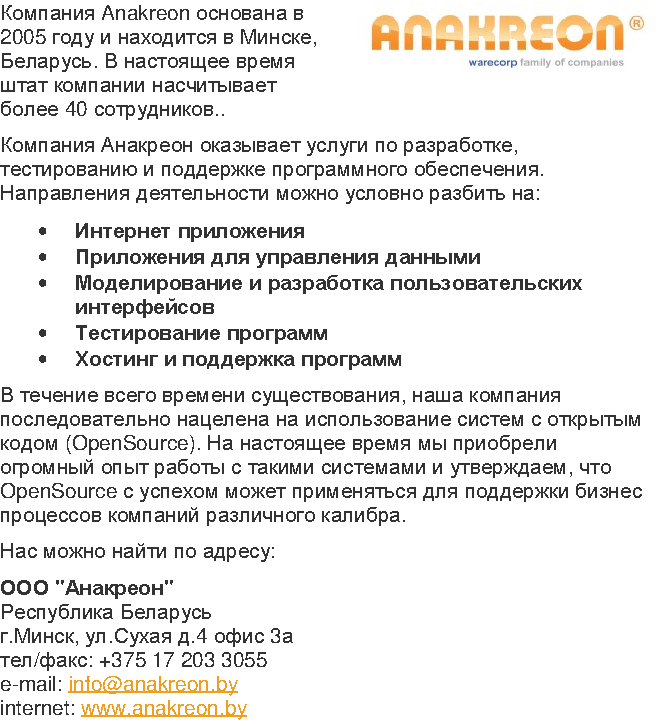
\includegraphics[width=11cm]{54_spons_anakreon.pdf}
\end{figure}
\end{document}



\documentclass[10pt, a5paper]{article}
\usepackage{pdfpages}
\usepackage{parallel}
\usepackage[T2A]{fontenc}
\usepackage{ucs}
\usepackage[utf8x]{inputenc}
\usepackage[polish,english,russian]{babel}
\usepackage{hyperref}
\usepackage{rotating}
\usepackage[inner=2cm,top=1.8cm,outer=2cm,bottom=2.3cm,nohead]{geometry}
\usepackage{listings}
\usepackage{graphicx}
\usepackage{wrapfig}
\usepackage{longtable}
\usepackage{indentfirst}
\usepackage{array}
\newcolumntype{P}[1]{>{\raggedright\arraybackslash}p{#1}}
\frenchspacing
\usepackage{fixltx2e} %text sub- and superscripts
\usepackage{icomma} % коскі ў матэматычным рэжыме
\PreloadUnicodePage{4}

\newcommand{\longpage}{\enlargethispage{\baselineskip}}
\newcommand{\shortpage}{\enlargethispage{-\baselineskip}}

\def\switchlang#1{\expandafter\csname switchlang#1\endcsname}
\def\switchlangbe{
\let\saverefname=\refname%
\def\refname{Літаратура}%
\def\figurename{Іл.}%
}
\def\switchlangen{
\let\saverefname=\refname%
\def\refname{References}%
\def\figurename{Fig.}%
}
\def\switchlangru{
\let\saverefname=\refname%
\let\savefigurename=\figurename%
\def\refname{Литература}%
\def\figurename{Рис.}%
}

\hyphenation{admi-ni-stra-tive}
\hyphenation{ex-pe-ri-ence}
\hyphenation{fle-xi-bi-li-ty}
\hyphenation{Py-thon}
\hyphenation{ma-the-ma-ti-cal}
\hyphenation{re-ported}
\hyphenation{imp-le-menta-tions}
\hyphenation{pro-vides}
\hyphenation{en-gi-neering}
\hyphenation{com-pa-ti-bi-li-ty}
\hyphenation{im-pos-sible}
\hyphenation{desk-top}
\hyphenation{elec-tro-nic}
\hyphenation{com-pa-ny}
\hyphenation{de-ve-lop-ment}
\hyphenation{de-ve-loping}
\hyphenation{de-ve-lop}
\hyphenation{da-ta-ba-se}
\hyphenation{plat-forms}
\hyphenation{or-ga-ni-za-tion}
\hyphenation{pro-gramming}
\hyphenation{in-stru-ments}
\hyphenation{Li-nux}
\hyphenation{sour-ce}
\hyphenation{en-vi-ron-ment}
\hyphenation{Te-le-pathy}
\hyphenation{Li-nux-ov-ka}
\hyphenation{Open-BSD}
\hyphenation{Free-BSD}
\hyphenation{men-ti-on-ed}
\hyphenation{app-li-ca-tion}

\def\progref!#1!{\texttt{#1}}
\renewcommand{\arraystretch}{2} %Іначай формулы ў матрыцы зліпаюцца з лініямі
\usepackage{array}

\def\interview #1 (#2), #3, #4, #5\par{

\section[#1, #3, #4]{#1 -- #3, #4}
\def\qname{LVEE}
\def\aname{#1}
\def\q ##1\par{{\noindent \bf \qname: ##1 }\par}
\def\a{{\noindent \bf \aname: } \def\qname{L}\def\aname{#2}}
}

\def\interview* #1 (#2), #3, #4, #5\par{

\section*{#1\\{\small\rm #3, #4. #5}}

\def\qname{LVEE}
\def\aname{#1}
\def\q ##1\par{{\noindent \bf \qname: ##1 }\par}
\def\a{{\noindent \bf \aname: } \def\qname{L}\def\aname{#2}}
}

\begin{document}
\title{Интервью с участниками}
%\author{}
\date{}
\maketitle

По сложившейся традиции в сборник материалов включены интервью, взятые представителями оргкомитета у участников конференции: как сразу после LVEE 2011, так и во время впервые проведенной в этом году выездной зимней сессии конференции LVEE Winter 2012. Интервью 2011 года было тематическим, посвященным использованию свободного программного обеспечения в сфере образования. Его участники принадлежат к разным странам и в той или иной степени имеют отношение к академическому процессу. Мы попросили их поделиться особенностями использования свободных программ в их вузах и услышали, какова ситуация в академических кругах Украины, Литвы и Венгрии.

\section[Григорий Злобин, Львов, Украина (LVEE 2011)]{Григорий Злобин, Львов, Украина \linebreak (LVEE 2011)}
%\begin{figure}[ht]
%\centering{\includegraphics[width=4cm]{49_spons_altoros.jpg}}
%\end{figure}

{\noindent \bf Григорий Злобин:} Я доцент Львовского университета, работаю на кафедре радиофизики факультета электроники. Уже шесть лет как у нас ведется подготовка студентов в направлении компьютерных наук. Возникло это благодаря тому, что раньше кафедра занималась разработкой программ машинного анализа электронных цепей, т.\,е. считалось, что мы имеем достаточный уровень профессиональной подготовки. А специальность, по которой мы готовим студентов "--- это <<Информационные системы>>.

{\noindent \bf L: Кем обычно работают выпускники этой специальности?}

{\noindent \bf Г:} Если честно, спектр очень широк. Работают и разработчиками, и системными администраторами, и разработчиками встроенного программного обеспечения, правда большая часть разрабатывает ПО для микроконтроллеров фирмы Cypress. Именно здесь наши выпускники имеют очень высокую подготовку, потому что для этих микроконтроллеров мало сделать ПО, нужно еще разработать аппаратную часть, как цифровую так и аналоговую. 

{\noindent \bf L: Учебный процесс по этой специальности как-нибудь задействует свободное ПО?}

{\noindent \bf Г:} Используется свободное ПО при чтении как общих курсов, так и при чтении спецкурсов. Общие курсы это <<Операционные системы>> и <<Системное программирование>>, а спецкурсы "--- здесь уже очень зависит от лектора. Поскольку мы по сути дела только в начале пути, то к сожалению наша кафедра не доросла до встраиваемых систем, где нужен Linux; пока мы занимаемся только микроконтроллерами. Правда, этому есть объяснение: очень большой объем заказов у фирм, занимающихся микроконтроллерами, и мы им не в состоянии дать столько студентов. Пока идет замыкание на микроконтроллеры Cypress, но я надеюсь, что мы будем двигаться дальше.

{\noindent \bf L: Программное обеспечение, используемое в вузе, это еще и средства обеспечения учебного процесса: те же текстовые редакторы и операционные системы...}

{\noindent \bf Г:} Да. Поскольку факультет наш принадлежит к естественным наукам, то курса информатики у нас просто нет. Но есть учебные практики после первого, второго, третьего курса, и это чудесная возможность вставить упреждающий по сути курс по ОС Linux, Openoffice, SciLab\ldots Могу похвастаться, что на практике мы используем оболочку <<Кузя>> "--- собственную разработку, наших студентов и для студентов.

{\noindent \bf L: А можно про нее пару слов?}

{\noindent \bf Г:}  Что было толчком? У нас на кафедре использовалась еще одна оболочка, сделанная под Windows для языка Паскаль. Я ее горячо поддерживал, а другие преподаватели относились с прохладой. Но когда у нас появилась компьютерная специальность, мы получили интересное явление: преподаватель, который читал программирование на Паскале, требовал, чтобы студенты этой оболочкой не пользовались. А студенты дома в ней работали, а потом на лабораторных работах сделанные программы сдавали в Turbo Pascal. И именно это натолкнуло их "--- студентов "--- на идею: если оболочка, сделанная именно под учебный процесс, дает возможность делать программы быстрее, давайте напишем ее сами. 

Поскольку <<Кузя>> использует компилятор gcc (и не только) "--- возможности его очень широкие. Правда, поскольку это работа просто по желанию "--- не все так хорошо движется, но мы с моим дипломником в следующем году собираемся сделать версию с веб-доступом. Так что ребята работают, это очень приятно\ldots У нас уже поддерживается шесть языков в интерфейсе, один из них белорусский, и есть арабский. Даже благодаря <<Кузе>> ребята, которые ее сделали, уже больше года работают разработчиками в фирме. 

Как ни парадоксально, изменить отношение к СПО помогла фирма Microsoft. Прошлой осенью я получил письмо от Сергея Байдачного с просьбой срочно, прямо завтра, предоставить резюме студентов, которые могли бы поехать на стажировку в Microsoft в США. Я быстро всех студентов проинформировал, ребята послали свои резюме, в т.~ч. и те, кто делали <<Кузю>>, причем один из них признался, что занимается СПО. И именно тот, который признался, прошел первый тур отбора. 

{\noindent \bf L: Это показатель :)}

{\noindent \bf Г:} Да. Противники СПО, когда об этом узнали, очень сильно озаботились. Это повлияло на преподавателей, у них начало меняться отношение. Хотя есть и другие примеры. Один из наших преподавателей написал методические указания к Matlab. Я предложил проверить, можно ли эти задания выполнить в Octave, и оказалось, что все выполняется. У нас в этом году открылась научно-исследовательская тема, в рамках которой мы собираемся сделать книгу <<Свободные системы компьютерной математики>>, и там будет раздел по Octave. Показательно, что я с этим же человеком дискутировал, когда он в других методических указаниях вставлял Matlab: <<Вот придет наш выпускник на производство и скажет: давайте купим Matlab, и я в нем такие вещи сделаю! А этого выпускника немедленно уволят, потому что Matlab стоит \$5000, а библиотека Simulink "--- \$45000. Они скажут, что им такие дорогие работники не нужны>>. А вот когда мы посмотрели, что то же самое можно сделать в Octave "--- это уже совсем другой поворот.

{\noindent \bf L: Какие требования у потенциальных работодателей ваших выпускников? Можно ли говорить о каком-то интересе работодателей к свободному ПО? Эта тема как-то просматривается?}

{\noindent \bf Г:} Ну, во-первых, фирмы, занимающиеся программированием во Львове, Softserve, Eleks, ведут разработки как под Windows, так и в СПО, и проявляют к этому большой интерес. Но на контакты с нами, тем не менее, идут не очень охотно, предпочитают напрямую работать со студентами. Потом, есть еще фирмы, нанимающие технический персонал для обслуживания облака в отдаленных от нас регионах, и работающие на открытом программном обеспечении. Но небольшая емкость рынка делает эту политику очень индивидуальной.

{\noindent \bf L: Как бы вы, коротко, охарактеризовали основные факторы в вузе, мешающие свободному программному обеспечению?}

{\noindent \bf Г:} Тотальная безответственность. Основная часть проприетарного программного обеспечения "--- пиратская, и несмотря на уголовный кодекс, который содержит очень жесткие уголовные нормы за пользование пиратским продуктом, вузы не трогают. И пока это так, вузы живут с позиции <<Мне все равно, а если даже будет проверка "--- проблема будет у ректора>>. Впрочем, я бы не хотел так уж обвинять своих коллег. Нужно еще учитывать, что уровень оплаты труда преподавателей не слишком соответствует решаемым задачам.

{\noindent \bf L: И последний вопрос: как вы заинтересовались свободным ПО сами?}

{\noindent \bf Г:} Это было лет 15 назад, еще до появления статьи в уголовном кодексе. Я как-то задумался: <<Неужели есть только Microsoft Office и больше ничего?>> Тогда мне под руки подвернулся Star Office, проприетарный продукт, бесплатный для учебных заведений. Я начал его пропагандировать и постепенно перешел в Linux. С Linux была проблема из-за той компьютерной техники, которую мы тогда имели. Некоторые легковесные дистрибутивы можно было поставить, но они не были локализированы. Это сразу означало, что мы не можем их использовать. А еще для нас было очень важным наличие украинского диалога. Долгое время фирма Microsoft игнорировала этот вопрос, считая, что достаточно русскоязычной версии. Только после появления локализированных дистрибутивов Linux они начали некоторую активность. Для некоторых регионов Украины наличие или отсутствие украиноязычного диалога не имеет никакого значения, но только не во Львове.

\section{Миколас Окулич-Казаринас, Вильнюс, Литва (LVEE 2011)}

%\begin{figure}[ht]
%\centering{\includegraphics[width=4cm]{49_spons_altoros.jpg}}
%\end{figure}

{\noindent \bf Миколас:} Я преподаватель университета им. Миколаса Ромериса в Вильнюсе. Уже три года как у нас создан новый факультет социальной информатики. Я работаю на кафедре информатики программных систем, и мы уже через год будем иметь первых выпускников "--- студентов по специальности <<Бизнес"=информатика>>.

{\noindent \bf L: Это достаточно новая специальность?}

{\noindent \bf М:} Новая, на стыке информатики и менеджмента. 

{\noindent \bf L: Как бы ты охарактеризовал потенциальный рынок труда для ваших выпускников?}

{\noindent \bf М:} Мое понимание этого вопроса чуть отличается от понимания некоторых других специалистов. Одна из предусмотренных специальностей "--- консультант по продажам информационных систем, но я надеюсь, что наши студенты также могут быть руководителями каких"=либо отделов или фирм, связанных с IT. Я хотел бы, чтобы высшее образование давало более высокое положение. А с другой стороны, т.\,к. мы имеем много предметов, связанных с бизнесом, мы не можем сделать из студентов хороших программистов, и я надеюсь сделать их настолько хорошими программистами, чтобы они могли сформулировать задачу для программистов"=профессионалов.

{\noindent \bf L: И как при такой специализации "--- свободное ПО находит какое-то применение в учебном процессе?}

{\noindent \bf М:} Конечно находит. Мы свободное программное обеспечение начали включать еще в 2004 году, т.\,е. до появления этой специальности и этого факультета. Что мы сделали "--- это инсталлировали OpenOffice на всех компьютерах кафедры, на которой я тогда работал, не удаляя ничего, что было прежде. Мне приходилось тогда преподавать социальную статистику, все задачи выполнялись на табличном процессоре. И когда я спросил: <<Какие табличные процессоры вы знаете?>> "--- около 5\% знали про OpenOffice. Из них около половины его раньше включали, и только один студент сказал, что имеет опыт работы. И я объяснил: <<Я вам преподаю статистические методы, и приходя на занятие, вы должны уже уметь пользоваться табличным процессором. В свободное время я могу показать вам программу, которую вы не знаете "--- OpenOffice. Вы можете выполнять задачи на чем угодно, но я вам предлагаю попробовать эту новую программу>>. После такого предложения один или два студента выполнили работу в Mircosoft Excel, а остальные выполнили их в OpenOffice или использовали обе программы. Причем я внимательно сравнивал качество этих работ "--- не было никакой корреляции между выбранной программой и качеством выполнения. Если бы студент начал работать с новой программой и столкнулся с проблемами "--- конечно он перешел бы обратно на уже известную программу. Не у всех хватило храбрости попробовать новую программу с первого занятия, но большинство из тех, кто раньше или позже попробовал, так до конца и делали задания в OpenOffice. Этот курс статистики, который я преподавал не для информатиков, а для совсем другой специальности, позволил мне убедиться, что в университете для непрограммистов можно без ущерба для учебного процесса использовать OpenOffice. Это был первый шаг.

Кроме того, еще до нового факультета у нас использовалась система Moodle. Мы сейчас развиваем систему сетевого обучения "--- чуть другой подход, чем дистанционное обучение, и в рамках этой системы у нас сервер работает на Linux. Однако общая  инфраструктура создана в университете еще до нас, она работает и нет смысла от нее отказываться. Может быть, если бы она была создана сейчас...

{\noindent \bf L: То есть свободное программное обеспечение находит применение и в сетевой инфраструктуре?}

{\noindent \bf М:} Когда появились информатики "--- появились задачи программирования. Программировали что-то локально. Я  создал сервер, к которому подключается каждый студент (но аутентификацию отдельную мы не делали, через LikwiseOpen наш сервер аутентифицируется в контроллере домена Active Directory), студенту создается автоматически акаунт в этом Linux-сервере, и веб-адрес. Каталог в домашнем каталоге студента отображается на веб-сервере в Apache. Первокурсник, получив задачу запрограммировать что-то на PHP, программирует и может сразу же показать что-то "--- в т.~ч. даже показать друзьям или позвонить домой. Возможно, в будущем~--- показать своему работодателю. С другой стороны, PHP "--- это язык, который дает слишком много возможностей, и я не уверен, что это хорошо с педагогической точки зрения.

{\noindent \bf L: А как у вас преподавательский состав относится к СПО?}

{\noindent \bf М:} Очень по-разному. Есть очень много хороших специалистов в области информатики, которые используют СПО, но без политического подтекста. Java, Netbeans, Eclipse\ldots Без разницы, Windows там или Linux. Есть такие, которые используют азартно, кто чувствует, что выучив что-то свободное, студент сможет потом предложить своему работодателю более дешевую и приспособленную систему. Задача университета "--- скорее подготовить таких специалистов, которые приносили бы деньги своему работодателю, а не указывали, что ему покупать. Есть люди, которые это понимают. Но есть конечно и такие, кто считает: <<Я столько версий этого монополиста изучал! Опять переучиваться? Нет уж, мне до пенсии и этого хватит>>. Самое неожиданное для меня было, когда один преподаватель сказал: <<Да, университет сэкономит очень много денег, но это же не я!>> Хотя я надеюсь, что это скорее исключения. 

Что больше всего радует "--- понимание на уровне администрации того, что сетевое обучение неотделимо от свободного ПО. Когда студент находится дома, он должен иметь все то же программное обеспечение, которое нужно для обучения, и мы не можем его обеспечить проприетарным ПО. И даже если какой-то поставщик сделает свой продукт для обучения бесплатным "--- все равно мы хотим, чтобы студент, чему-то научившись, сразу мог использовать этот продукт для своей работы, для частного бизнеса, для чего-то еще\ldots А для этого подходит только открытое программное обеспечение. 

Когда преподаватели почувствовали поддержку сверху, от администрации "--- возмущений стало все меньше и меньше. С другой стороны, свободное ПО совершенствуется быстро, и то что было несколько лет назад "--- хуже чем есть сейчас. И еще, когда появился compiz, люди не интересовавшиеся Linux, собрались в преподавательской смотреть на поворачивающийся куб\ldots :) 


{\noindent \bf L: Да, надо сказать, что хотя аппаратное ускорение графики придумали не в Linux, зато в Linux его внедрили быстрее всего. И заметнее. }

{\noindent \bf М:} Да. С другой стороны, есть люди, которые много лет используют Windows, и они не хотят ничего менять, считая это стабильностью. 

{\noindent \bf L: А как вообще в Литве себя чувствует свободное программное обеспечение?}

{\noindent \bf М:} Рост есть. Я "--- один из учредителей ассоциации открытого кода (АКЛ), мы раньше несколько лет участвовали в региональной выставке информационных технологий InfoBalt. В первом году реакция была: <<Что, бесплатно?>> Люди не понимали. На следующий год "--- <<Да-да-да, я слышал>>. Потом "--- <<Я использовал>>. А на следующий год уже толпа народу: <<Я использую Ubuntu>>. Мы чувствовали, что с каждым годом все больше людей приходило, которые понимали, и что они все больше понимали. Это было очень ярко выраженно. Студенты тоже много используют Ubuntu, даже в тех университетах, которые ее не используют. Но на государственном уровне все пока не так хорошо. Есть очень много хороших специалистов в государственных структурах, которые хотели бы двигаться в этом направлении. У монополистов есть свои методы саботировать эти процессы.

{\noindent \bf L: А как ты сам заинтересовался свободным ПО?}

{\noindent \bf М:} В детстве я программировал. Был Turbo Pascal и  Quick Pascal. Более крупная фирма, победившая в университете, использовала не вполне честные методы продвижения своего продукта, заявленные возможности оказались не до конца реализованы, и мне это не понравилось. А потом я хотел иметь легальное программное обеспечение. Купил на какой-то выставке редактор Ami Pro, за \$100, и вдруг оказалось, что функциональность идентична редактору от Mircosoft, но я не могу им пользоваться, потому что невозможен ни с кем никакой обмен данными. Я понял, что вся система функционирует против потребителей. И потом, когда я работал в ассоциации потребителей, моя специализация была "--- защита потребителей от монополистов, главные направления "--- в IT  и в отоплении.

{\noindent \bf L: Т.~е. интерес к свободному ПО родился из соображений защиты потребителя?}

{\noindent \bf М:} Да. Причем в начале 2000-х, когда я первый раз инсталлировал себе Linux, я знал, что будут проблемы с драйверами, будет тяжело, но я хотел показать на своем примере, что это возможно. Наверное, полгода прошло, пока у меня начало работать все, что я хочу, а еще через полгода я начал чувствовать, что  обратно вернуться не хотелось бы. Сейчас\ldots У нас выпускают дистрибутив Baltix на базе Ubuntu, когда просто ставишь компакт"=диск, нажимаешь <<Инсталлировать>>, и имеешь полный набор программ для своего десктопа, в отличие от закрытого программного обеспечения, где инсталлируешь операционную систему, потом офисный пакет, потом антивирусы всякие\ldots Понимаешь, что в Linux  на порядок быстрее и проще все сделать. Сейчас уже совсем другая ситуация, все в пользу Linux. А почему люди не переходят?

{\noindent \bf L: А почему?}

{\noindent \bf М:} А потому, что люди консервативны, наверное. Я администрировал компьютеры в одной фирме, учредитель поручил проверить, все ли у нас легально, и оказалось, что Microsoft Office не оплачен. Тогда я предложил директору OpenOffice, бесплатно, и он конечно же был за. Но я опасался, что многие сотрудники будут против, и проинсталлировав его, не сказал им, что это новая программа, а сказал: <<Я обновляю наш офис>>. Все спокойно это восприняли, и даже сказали, что у них на порядок стало лучше управление таблицами. Люди боятся даже не программы, а нового названия.

\section[Даниэль Надь, Будапешт, Венгрия (LVEE 2011)]{Даниэль Надь, Будапешт, Венгрия \linebreak (LVEE 2011)}

%\begin{figure}[ht]
%\centering{\includegraphics[width=4cm]{49_spons_altoros.jpg}}
%\end{figure}

{\noindent \bf Даниэль Надь:} Каждый второй семестр я веду курсы по криптографии в Будапештском университете имени Лоранда Этвёша на факультете естественных наук, на кафедре операционных исследований.

{\noindent \bf L: Каких специалистов готовит кафедра ?}

{\noindent \bf Д:} В основном математиков, и кроме этого есть еще такая специальность, <<математик-программист>>. Ожидаемое место их последующей работы "--- это либо академическая сфера, либо индустрия информационных технологий.

{\noindent \bf L:  Как в учебном процессе используется свободное ПО?}

{\noindent \bf Д:} Достаточно широко. В общем-то, во всех сферах деятельности. Терминалы, которыми пользуются студенты, на Linux. Сейчас это тонкие клиенты. Очень много свободного софта типа Octave, но в любом случае есть конечно и коммерческие приложения, которые в академической сфере очень распространены. 

{\noindent \bf L: В том числе и потому, что приходится ориентироваться на рынок труда?}

{\noindent \bf Д:} Частично да, а частично потому, что некоторым приложениям, типа Mathematica, пока еще полноценной свободной замены нет. Но там где можно, совободное ПО широко используется. Большинство статей пишется в \TeX, графики рисуются в gnuplot "--- это две программы, которые знает каждый, кто прошел через кафедру математики.  

Unix-подобные системы, еще до того, как они стали свободными, получили достаточно широкое распространение в венгерских вузах, потому что еще в начале девяностых или даже в конце восьмидесятых по некоторым западным грантам было получено оборудование с Solaris от Sun, AIX от IBM, поэтому Unix в венгерской системе образования уже очень давно, и менять его по частям на свободное ПО было легко и безболезненно для преподавательского состава и для научных работников, и естественно, для студентов также. Резкого перехода в духе <<Раньше мы использовали что-то другое, а теперь будем использовать Linux>> "--- не было. Постепенно, терминал за терминалом это старое железо от Sun менялось на Linux-станции.

{\noindent \bf L: А как сам ты заинтересовался свободным ПО, помнишь?}

{\noindent \bf Д:}  Это было в другом университете. Я сам учился в техническом университете, и там я впервые увидел Интернет, как таковой, старые Unix'ы, которые тогда еще были новыми. Мне очень нравилась система Silicon Graphics. И когда в одной из лабораторий поставили на клиенты Linux, я понял, что на дешевом домашнем компьютере, который я могу иметь, тоже может быть что-то похожее. Тогда я начал интересоваться Linux, и\ldots пошло-поехало.

{\noindent \bf L: Как вообще свободное ПО чувствует себя в Венгрии?}

{\noindent \bf Д:} Достаточно комфортно. В Венгрии есть люди с большим энтузиазмом и большой энергией, которые его распространяют, так что венгерская локализация  достаточно качественная. Потом, по причине восточно-европейского безденежья очень многие принимают решение пользоваться свободным ПО. Единственное, где у свободного ПО серьезные трудности "--- это крупные компании и государственные учреждения. С бесплатного "--- и откатов нет :)

\section[Виталий Липатов, Санкт-Петербург, Россия (LVEE Winter 2012)]{Виталий Липатов, Санкт-Петербург, \linebreak Россия (LVEE Winter 2012)}

Незадолго до конца LVEE Winter 2012 мы взяли интервью у Виталия Липатова "--- члена команды разработчиков  дистрибутива ALT Linux и генерального директора компании Etersoft, известной в первую очередь своей собственной коммерческой версией проекта wine. Вопросы от имени LVEE задавали Дмитрий Костюк и Инна Рыкунина.

{\noindent \bf LVEE: Вопрос, который всегда легко задавать: а как получилось, что ты заинтересовался свободным ПО?}

{\noindent \bf Виталий Липатов:} Где-то году в 92-м или 93-м папа купил мне книжку <<UNIX "--- универсальная среда программирования>>. Тогда я её прочитал и ничего не понял, большие системы в начавшуюся эпоху персональных компьютеров казались далёкими, как динозавры. А лет через шесть, когда я заканчивал ВУЗ, меня пригласили работать в центральный НИИ судовой электротехники в лабораторию, где разрабатывалось программное обеспечение для пригородной электрички. Я попал в проект не с самого начала, и когда пришёл, выбор операционной системы уже был сделан, а выбирали между QNX и Linux. 

{\noindent \bf L: А что вообще операционная система делает в электричке?}

{\noindent \bf В:} Она стоит на контроллерах, которые управляют тормозами, дверями, скоростью движения,  пультом машиниста (там монитор, который выводит все показатели, лампочки зажигаются предупредительные)\ldots в поезде множество подсистем, они традиционно разрабатываются разными организациями, как, например, система безопасности электропоезда. Интересно, что тогда мы одни из первых начали применять Ethernet, у нас был проложен кабель сквозь весь поезд. Ранее обычно применялись разные стандартные и нестандартные протоколы на базе последовательного интерфейса.

{\noindent \bf L: Вагоны в локальной сети...}

{\noindent \bf В:} Да, это был 2000 год. И QNX не выбрали "--- потому, что если умножить стоимость лицензии QNX на количество вагонов, которые предполагалось выпускать серийно\ldots Выбрали Linux, тогда это был Slackware 3.5 с ядром 2.0.34, по-моему. Тогда уже, конечно, существовали и другие дистрибутивы...

{\noindent \bf L: Но люди любили Slackware, поэтому электричка работала на ней.}

{\noindent \bf В:} Это была первая Linux-система, которую я увидел, и она меня очень впечатлила. Так я познакомился с Linux. Немного поработав с ним, почувствовал, что освоить это невозможно. Бесчисленное количество команд с разными параметрами, и совершенно нереально запомнить, что у <<cp>>  есть параметр <<-a>>, а у <<tar>> нужно писать <<xvfz>>, чтобы что-нибудь распаковать\ldots Но потом мозг как-то со всем этим справился, и я понял, что это та самая система, о которой я всегда подсознательно мечтал. Недостатков даже не было заметно. И вообще, тогда в Linux не было недостатков, они появились намного позже :)

{\noindent \bf L: Тогда их ещё не успели написать :)}

{\noindent \bf В:} И вот, мы для 386 процессоров сделали систему, и всё очень быстро работало.

{\noindent \bf L: Проект был закончен?}

{\noindent \bf В:} Да, электричку мы сделали, но её не пустили в серию, к сожалению. Был изготовлен поезд в шесть вагонов, он прошёл все испытания.

{\noindent \bf L: В общем, интерес к Linux заметно пережил этот проект. А собственно интерес к свободному ПО?}

{\noindent \bf В:} Он появился немного позже. Эта мысль достаточно долго входила в сознание. Я перечитывал ту книжку про Unix, а ещё как раз недавно появился Интернет, и я узнал, что есть другие люди, которые под это что-то пишут, и втянулся. А потом попал в ALT Linux Team.

{\noindent \bf L: А кстати, как это произошло?}

{\noindent \bf В:} Для дальнейшей деятельности нам потребовался новый дистрибутив, а выбирали мы почему-то между только появившимся Mandriva RE Spring 2001 и ASP Linux. Я долго выбирал. ASP Linux выглядел красиво и профессионально. Но интуитивно меня тянуло к собранному в ALT Linux дистрибутиву. Сейчас я уже не помню подробностей. Возможно, уже тогда я заметил наличие сообщества разработчиков.

Параллельно с НИИ я работал в компании, где  писал конфигурации для 1С, причем с нуля. Работал один, написал их три штуки для разных направлений деятельности, заодно что-то администрировал "--- скучная такая деятельность для творческого человека. Там у меня был сервер на Linux, на котором лежали файлы баз данных для 1С:Предприятия. А и одновременно это был мой рабочий компьютер и мне нужно было на нём писать код, поэтому я в итоге озаботился, а как бы запустить 1С:Предприятие в Linux. Это был год, наверное, 2002 или 2003.  

{\noindent \bf L: Вот, оказывается, откуда растёт WINE@Etersoft!}

{\noindent \bf В:} Это уже позже, в 2004 году на выставке Softool в Москве мы от имени свежеорганизованного Etersoft показали, что на  WINE@Etersoft запускается 1С:Предприятие. Причём показывали, подключаясь к Linux-серверу с тонкого клиента, то есть в режиме терминального доступа. А в то время я только знал, что есть такой пакет wine, позволяющий запускать Windows-программы, попробовал его\ldots Долго подбирал настройки и библиотеки, и в итоге 1С:Предприятие запустилось. Работать оказалось не совсем возможным, слишком много багов\ldots Тогда я уже был пользователем ALT Linux. В то время wine там собирал генеральный директор ALT Linux Алексей Евгеньевич Новодворский. Пару раз он исправлял пакет по моим замечаниям, а потом прислал письмо в рассылку разработчиков ALT Linux: <<Уважаемые коллеги, представляю вам нового сопровождающего пакет wine Виталия Липатова, прошу любить и жаловать>>. То есть меня как бы поставили перед фактом. А я был очень благодарен за оказанное доверие\ldots 

Но Etersoft стал заниматься wine позже: когда мы наконец открылись и думали внедрять ALT Linux в офисах, оказалось, что никому это вообще-то не нужно, потому что для Linux нет необходимых прикладных программ. Тут мы поняли, что в офисах должно работать 1С:Предприятие, причем не просто запускаться, а реально работать, в сетевом режиме, когда есть много пользователей. Именно это востребовано, а особенно на терминальном сервере, т.\,е. в режиме, который позволяет получить от 1С:Предприятия версии 7.7 максимум производительности. Мы на это нацелились, сделали, и в конце 2005 года начали продавать первые версии. Собственно, первую версию продали уже чуть ли не под новый год.

{\noindent \bf L: Новогодний подарок. Оно работало?}

{\noindent \bf В:} Весьма относительно\ldots Но у нас были принципы, которых мы придерживались:  бухгалтерия в нашей компании использовала \linebreak 1С:Бухгалтерию, и мы запускали её под Linux.

{\noindent \bf L: А кстати, как по поводу изменений в wine? Этот проект ведь прославился тем, что периодически происходят изменения в апстриме, когда что-то внезапно может сломаться. Насколько часто и насколько болезненно такая ситуация бьёт по коммерческой версии?}

{\noindent \bf В:} Раньше, много лет назад, когда релизов wine почти не было, просто забирали из cvs какой-то срез кода и пытались им пользоваться. Стабильность действительно оставляла желать лучшего. Но потом разработчики wine перешли к концепции, что после любого изменения код не должен деградировать, стали требовать этого от разработчиков, появилась система тестирования. Требования ужесточили, в итоге сейчас wine перешёл на чёткие релизы. Каждый день новые коммиты, и каждую неделю выходит новый релиз. Причем невозможно прислать изменения, если ты перед этим не написал тест, который подтвердит, что  проблема есть, а после твоего исправления она исчезает. Эти тесты требуют не просто так "--- в проекте работает автомат, который прогоняет их на десяти разных конфигурациях Windows и Linux и проверяет, нет ли деградации.

Из-за достаточно серьёзного тестирования новых патчей сейчас так сильно всё не ломается. Но до последнего времени мы свою текущую ветку разработки синхронизировали очень редко. У нас мало ресурсов, поэтому мы выбирали некоторую стабильную для нас версию оригинального wine. Дальше мы уменьшали количество багов в ней, не синхронизируясь с основной веткой. Но за последние два года wine дошел наконец до версии 2.0. Мы синхронизировались и написали робота, который периодически  переносит изменения из апстрима в нашу ветку разработки. После сборки прогоняются тесты, проверяется, не появилось ли регрессий. Не так идеально, как в оригинальном wine, но всё-таки тесты мы запускаем.

{\noindent \bf L: Вы передаёте свои  исправления в апстрим?}

{\noindent \bf В:} Конечно. Раньше "--- больше, апстрим wine был менее строгим. И сейчас иногда принимают что-то. Теоретически мы должны от этого выигрывать, но на практике этого не замечаем. Количество хаков, которые мы не можем послать, просто потому они не будут приняты, больше, чем то, что у нас приняли. Мы специально для патчей, которые у нас должны бы принять, ведём отдельную ветку. Она свободная, и wine в ALT Linux собирается именно из неё. На нашем ftp-сервере доступны сборки и под другие системы.

{\noindent \bf L: Насколько широко расходится  WINE@Etersoft как коммерческий продукт?}

{\noindent \bf В:} Я так понимаю, что это зависит от роста популярности Linux. Процесс взаимосвязанный. Иногда я слышу, что без нашей деятельности по помощи в запуске Windows-программ в таком объёме движения не было бы. Раньше, когда компанию 1С просили сделать версию под Linux, они отвечали: <<У нас там нет пользователей>>. Мы этот порочный круг разомкнули, и появились пользователи под Linux. Теперь в компании 1С сделали Linux"=версию, пока только серверную часть, их самый дорогой продукт. Клиент может быть запущен либо под Windows, либо можно подключиться через браузер, но это доступно не для всех конфигураций, и не вся функциональность доступна, поэтому наше решение по запуску Windows"=клиента остаётся востребованным.

На этом проекте нам не удаётся много зарабатывать, и, соответственно, быстро его развивать. Специфика такова, что готовых разработчиков не существует, и новых сотрудников нам приходится обучать практически с нуля "--- как писать код, как отлаживать, какие приёмы использовать для поиска ошибок в бинарном коде. Деятельность не очень благодарная и мало кому нравится.

{\noindent \bf L: А вы не эксплуатируете практикантов?}

{\noindent \bf В:} Вообще-то студенты проходят к нам на практику, но в основном те, кто уже у нас работает. А так\ldots В городе множество компаний, предлагающих более высокие зарплаты, но у нас есть другие преимущества:  свободный график, особая атмосфера, интересная работа\ldots Для сотрудников разработана целая система,  интегрированная  Bugzilla, которая высчитывает рабочее время, учитывает решённые задачи.

{\noindent \bf L: Если в двух словах коснуться ваших продуктов, менее известных широкой публике, чем wine?}

{\noindent \bf В:} Наши другие продукты "--- во многом эксперимент, что же ещё будет востребовано по теме миграции на Linux. Есть SQL-транслятор SELTA@Etersoft, который позволяет отказаться от Microsoft SQL Server. Версию 2.0 хотим сделать в виде прокси-сервера, со стороны сети выглядящего точно как MS SQL. Там много сложностей: хранимые процедуры, встроенные функции\ldots Это пример полностью нашего коммерческого продукта, построенного, правда, на нашей собственной сборке PostgreSQL, которая конечно же свободно доступна. А пример нашего свободного продукта "--- UniOffice, который  подменяет Microsoft Office на OpenOffice для VBA-приложений. Есть у нас и решение для организации терминального доступа "--- RX@Etersoft, основанное на NX. Ещё у нас есть совершенно другая деятельность: мы делаем промышленные системы управления. 

{\noindent \bf L: Например?}

{\noindent \bf В:} Например, мы разрабатываем ПО для электростанций в России. К нам обратилась компания, по заказу которой производились преобразователи частоты в Китае. Там делали железо и программу управления к нему под Windows. Она закрывалась каждые несколько часов из-за различных ошибок… А тут требовалась бесперебойная работа в течение года. Там всё очень серьёзно, преобразователь управляет нагнетателем, подающим воздух для горения газа, и если пропорция смеси нарушается, всё чревато аварийной ситуацией. Нас нашли, уговорили, мы в очень сжатые сроки сделали этот заказ, последние штрихи наводили уже на электростанции. И вот система уже более 5 лет работает, без сбоев. Мы делаем и другие подобные системы управления для судов:. Не системы навигации, там свои поставщики, а мониторинг, контроль, системы сигнализации, пульты в рубку и др. И в том и том случае на базе ALT Linux. 

{\noindent \bf L: На нём плавают корабли и работают электростанции. А как твои сегодняшние впечатления? На что похоже LVEE?}

{\noindent \bf В:} Достаточно необычно. Я участвовал в двух видах мероприятий: тех, что проводятся ALT Linux "--- в основном с людьми, близкими к ALT Linux Team, в них ещё сильна академическая составляющая. И другого типа "--- те, что проводятся крупными спонсорами, такими как IBM или Sun, для своих целей, в фешенебельных отелях,  на тысячи людей.

У вас отличается формат и люди по глубине задействованности: совершенно другой пласт, с которым на тех мероприятиях не сталкиваешься. Мне очень понравилось мероприятие, рад был встретить такое количество небезразличных к свободному ПО людей.

\end{document}

\newpage

\makeatletter
\let\enddocument\@lvee@enddoc
\let\input\@lvee@input
\makeatother

\eof


